% The contents of this file is 
% Copyright (c) 2009-2011  Charles R. Severance, All Righs Reserved

%\documentclass[10pt,b5paper]{book}
\documentclass[11pt]{book}
% \usepackage[width=5.25in,height=7.50in,hmarginratio=3:2,vmarginratio=1:1]{geometry}
\usepackage[size=journal,gutter=0.75in,trim,bleed]{createspace}

\usepackage{pslatex}
\usepackage{url}
\usepackage{fancyhdr}
\usepackage{graphicx}
\usepackage{amsmath, amsthm, amssymb}
\usepackage{exercise}
\usepackage{makeidx}
\usepackage{setspace}
\usepackage{hevea}
\usepackage{alltt}
\usepackage{upquote}
\usepackage{kotex}

\newcommand{\thetitle}{Python for Informatics: Exploring Information}
\newcommand{\theversion}{0.0.9-d2}

\makeindex

\begin{document}

\frontmatter

% The contents of this file is 
% Copyright (c) 2009-  Charles R. Severance, All Righs Reserved

% LATEXONLY

\input{latexonly}

\newtheorem{ex}{Exercise}[chapter]

\begin{latexonly}

\renewcommand{\blankpage}{\thispagestyle{empty} \quad \newpage}

\thispagestyle{empty}

\begin{flushright}
\vspace*{2.0in}

\begin{spacing}{3}
{\huge 정보교육을 위한 파이썬}\\
{\Large 정보 탐색}
\end{spacing}

\vspace{0.25in}

Version \theversion

\vspace{0.5in}


{\Large
저자: Charles Severance\\
번역: 이광춘, 한정수 \\
(xwmooc)
}

\vfill

\end{flushright}

%--copyright--------------------------------------------------
\pagebreak
\thispagestyle{empty}

{\small
Copyright \copyright ~2009- Charles Severance.


출판 이력:

\begin{description}

\item[2014년 9월:] xwmooc 프로젝트 일환으로 \emph{''정보과학을 위한 파이썬''} 으로 제목 정하고 한국어로 번역 공개

\item[2013년 10월:] JSON로 전환, OAuth 사용. 13장, 14장에 주요 개정
신규 시각화 장 추가.

\item[2013년 9월:] Amazon CreateSpace 책 출판

\item[2010년 1월 :] 미시건 대학 Espresso Book Machine 사용 책 출판

\item[2009년 12월:] \emph{Think Python: How to Think Like a Computer Scientist}에서 2장 {\verb"~"} 10장까지 주요 개정 \\
\emph{Python for Informatics: Exploring Information}을 위해 1장, 11장 {\verb"~"} 15장 저작

\item[2008년 6월:] \emph{Think Python: How to Think Like a Computer Scientist} 제목 바꾸고, 주요 개정.

\item[2007년 8월:] \emph{How to Think Like a (Python) Programmer} 제목 바꾸고, 주요 개정.

\item[2002년 4월:] \emph{How to Think Like a Computer Scientist} 초판 공개

\end{description}

\vspace{0.2in}

이 책은 크리에이티브 커먼즈 라이선스 3.0 (Creative Commons Attribution-NonCommercial-Share Alike 3.0)으로 인가되었다.
라이선스의 자세한 사항은 \url{creativecommons.org/licenses/by-nc-sa/3.0/}에 기재되어 있다.
저작권 상세 부록에서 저자가 생각하는 상업적, 비상업적 이용 그리고 라이센스 면제를 생각하는 바를 확인할 수 있다.
이책의 \emph{Think Python: How to Think Like a Computer Scientist}의 \LaTeX\ 소스는 
\url{http://www.thinkpython.com}에서 이용가능하다.

\vspace{0.2in}

} % end small

\end{latexonly}


% HTMLONLY

\begin{htmlonly}

% TITLE PAGE FOR HTML VERSION

{\Large \thetitle}

{\large 
Charles Severance}

Version \theversion

\setcounter{chapter}{-1}

\end{htmlonly}

%% The contents of this file is 
% Copyright (c) 2009- Charles R. Severance, All Righs Reserved

\chapter{한국어판 서면}

첫 인터넷 웹 브라우저를 만든 마크 앤더슨은 소프트웨어가 세상을 먹고 있다("Software is eating the world")는 자극적인 표현으로 2011년 월스트리트 저널에 에세이를 썼고, 카네기멜론 대학의 쟈넷 윙 교수는 이론적 사고(Theoretical Thinking), 실험적 사고(Experimental Thinking))와 더불어 정보적 사고(Computational Thinking)가 현재도 그렇지만 앞으로 인간의 사고를 지배하는 중추적인 역할을 할 것을 주장했다. 이들의 결과는 정보적 사고를 배운 사람과 소프트웨어를 이해하고 활용하는 사람과 그렇지 못한 사람과의 차이는 산업경제의 빈부격차보다 더 큰 디지털 경제의 정보 불평등(Digital Divide)를 야기할 것으로 예측했다.

정부는  ’14년 7월 세계 경제, 사회 환경이 소프트웨어 중심사회로 급격히 변화하고 있으며, 소프트웨어가 혁신과 성장, 가치창출의 중심이 되고, 개인•기업•국가의 경쟁력을 좌우하는 중요한 역할을 하고 있음에도 불구하고, 우리나라는 범정부적, 국민적 관심이 미흡한 상황이라고 진단하고, 미국, 영국, 이스라엘 등 선진국과 마찬가지로, 초•중•고에서 소프트웨어를 필수로 이수할 수 있는 방안을 강구하고 있다.

하지만, 지금까지의 관심은 소프트웨어만 집중되어 왔고, 정보 및 데이터에 대한 부분은 상대적으로 소홀히 다뤄왔다. 
''Python for Informatics'' 번역을 통해서 컴퓨터 언어를 쉽고 빠르게 그리고 정보 및 데이터에 대한 부분도 효과적으로 학습할 수 있을 것으로 기대한다.

이광춘 한정수 (xwmooc)\\
http://www.xwmooc.net\\
경기도 과천\\
2014년 9월

\chapter{서면}

\section*{정보교육을 위한 파이썬: 공개된 책 리믹싱}
''출판 혹은 소멸(publish or perish)''를 들어온 학자는 자신만의 신선한 창조로 무에서 만들어내는 것은 무척이나 자연스럽다.
이책은 아무 것도 없는 것에서 시작하는 대신에 Allen B. Downey, Jeff Elkner와 협력자들이 저작한 \emph{Think Python: How to Think Like
a Computer Scientist} 책을 ''리믹싱(re-mixing)''하는 실험이다.

2009년 12월, 미시건 대학에서 연속해서 5 학기 {\bf SI502 - Networked Programming}을 준비중이었고,
알고리즘과 추상화를 이해하는 대신에 데이터 탐색에 집중하는 파이썬 교과서를 쓸 시점이라고 정했다.
SI502 목표는 파이썬을 사용하여 사람들에게 평생 데이터를 다루는 기술을 가르치는 것이다.
대신에, 핵생들 중 누구도 전문적인 컴퓨터 프로그래머를 계획한 사람은 없었다.
대신에 학생들은 도서관원, 관리자, 변호사, 생물학자, 경제학자가 되고자 했는데 자신만의 영역에서 능숙하게 기술을 사용하고자 했다.

수업을 위해서 결코 완벽한 데이터 지향 파이썬 책을 발견할 것 같지 않아서 그런 책을 저작하려고 시작했다.
휴가 기간동안 아무것도 없는 상태에서 새로운 책을 시작하기 3주전 다행스럽게도 교수 회의에서, Atul Prakash 박사가
지난 학기 파이썬 과정을 가르치는데 사용한 \emph{Think Python} 책을 보여주었다.
간결하고 직접적인 설명에 학습하기 쉬운 것에 초점을 맞춘 잘 쓰여진 컴퓨터 과학 교과서였다.

전반적인 책의 구조는 가능한 빠르게 데이터 분석 문제를 다루고, 처음부터 데이터분석에 관한 실전 예제와 연습문제로 바꾸었다.

2-10 장은 \emph{Think Python} 책과 매우 유사하지만 주요 변경사항이 있다.
숫자 중심의 예제와 연습문제는 데이터 지향 연습으로 대체했다.
주제는 순차적으로 제시되어서 점차적으로 정교한 데이터 분석 솔류션을 구축하도록 했다.
{\tt try}, {\tt except} 같은 주제는 앞으로 가져와서 조건문 장의 일부에 제시했다.
함수는 추상화의 첫 수업에 소개되기 보다는 프로그램 복잡성을 다루는데 필요할 때까지 매우 가볍게 다루었다.
거의 모든 사용자 정의 함수는 4장 밖으로 예제 코드와 연습문제를 제거했다.
단어 ``재귀(recursion)''\footnote{물론 이번 줄은 제외다.}는 책의 어디에도 나타나지 않는다.

1장, 11-16장의 모든 콘텐츠는 완전히 새로운 실무 사용과 데이터 분석을 위한 파이썬 간단한 예제에 집중했다.
데이터 분석은 검색과 파싱를 위한 정규 표현식, 사용자 컴퓨터의 작업 자동화, 네트워크 상에서 데이터 가져오기,
데이터로 웹페이지 스크랩핑, 웹서비스 사용하기, XML과 JSON 데이터 파싱, 그리고 SQL(Structured Query Language)을 사용한
데이터베이스 생성 및 사용을 포함한다.

이 모든 변화의 궁극적인 목적은 컴퓨터 과학에서 인포매틱스(informatics)로 전환이고, 설사 전문적인 프로그래머가 되지 않을 지라도
유용한 첫 기술 과목안으로 의제를 포괄하는 것이다.

이책이 흥미롭고 좀더 탐색하고자 하는 학생은 Allen B. Downey 의 \emph{Think Python} 책을 봐야한다.
두 책간에 많이 겹치는 부분이 있어서, \emph{Think Python}에서 다루는 기술적인 프로그래밍과 알고리즘적 사고에 대한 기술을 빠르게 습득할 것이다.
그리고, 책의 저작 스타일 매우 유사해서, 최소의 노력으로 \emph{Think Python}을 통해서 빠르게 나아갈 수 있다.

\index{Creative Commons License}
\index{CC-BY-SA}
\index{BY-SA}

\emph{Think Python} 저작권자로서, Allen은 GNU 공개 문서 라이센스가 적용된 본인의 책에서 이 책에 적용된 좀더 최근의 크리에이티브 커먼즈 저작자 명시, 동일한 라이선스 적용(CC-BY-SA)변경하도록 허가를 주었다. 
공개 문서 라이센스가 GFDL에서 CC-BY-SA(예, 위키피디아) 바뀌는 추세를 따르는 것이다.
CC-BY-SA 라이선스를 사용하는 것은 책에 대한 강력한 카피레프트 전통을 유지하면서, 새로운 저자가 재사용해서 자신의 목적에 맞춰 사용하도록 좀더 직접적으로 만드는 것이다.
이 책이 왜 공개 저작물이 미래 교육에 매우 중요하다고 느끼고, 책을 공개 저작권 아래에서 이용가능하게 만든 앞을 내다보는 결정을 내린 Allen B. Downey와 Cambridge University Press에 감사드린다. 저자 노력의 결과에 기뻐하고, 독자는 \emph{모두의} 공동 노력에 즐거워하길 희망한다.

이 책과 관련된 저작권 이슈를 해결하고 처리하는데 인내를 가지고 도움과 안내를 주신 Allen B. Downey와 Lauren Cowles 분께 감사를 표한다.

Charles Severance\\
www.dr-chuck.com\\
Ann Arbor, MI, USA\\
2013년 9월 9일

Charles Severance는 미시건 대학 정보 학교 부교수다.

\clearemptydoublepage

% TABLE OF CONTENTS
\begin{latexonly}

\tableofcontents

\clearemptydoublepage

\end{latexonly}

% START THE BOOK
\mainmatter



% START THE BOOK
\mainmatter

%% The contents of this file is 
% Copyright (c) 2009-  Charles R. Severance, All Righs Reserved

\chapter{왜 프로그래밍을 배워야 하는가?}

컴퓨터 프로그램을 만드는 행위(프로그래밍)는 매우 창의적이며 향후 뿌린 것 이상으로 얻을 것이 많다. 프로그램을 만드는 이유는 어려운 자료분석의 문제를 해결하려는 것에서부터 다른사람의 문제를 해결해주는 재미를 느끼는 것까지 다양한 이유가 있다. 이 책에서 모든 사람이 어떻게 프로그램을 만드는지를 알고, 프로그램을 만드는지를 알게되면, 새로 습득한 프로그래밍 기술로 원하는 것을 해결할 수 있는 것을 배우게 된다.

우리의 일상은 노트북부터 핸드폰까지 다양한 컴퓨터에 둘러싸여 있다. 이러한 컴퓨터가 개인비서로 우리를 위해서 많은 일을 대신해 준다고 생각한다. 일상생활에서 접하는 컴퓨터 하드웨어는 우리에게 "다음에 무엇을 하면 좋겠습니까?" 라는 질문을 지속적으로 물어보게 만들어 졌다.


 
\beforefig
\centerline{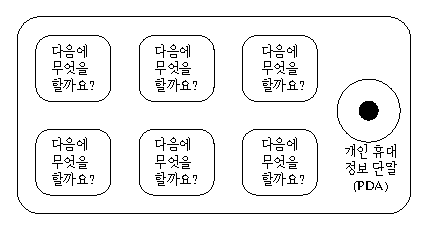
\includegraphics[height=1.00in]{figs2/pda.eps}}
\afterfig

프로그래머는 운영체제와 하드웨어에 응용 프로그램을 만들었고, 결국 많은 것들을 도와주는 PDA(Persoanl Digital Assistant)로 진화했다. 컴퓨터는 빠르며, 큰 저장소를 가지고 있어 우리가 컴퓨터에게 "다음꺼 실행해(do next)를 컴퓨터가 이해할 수 있는 말로 지시를 하게되면 우리에게 매우 유용할 수 있다.

예를 들어, 다음의 세 문단을 보고 가장 많이 나오는 문단의 단어를 찾아보고 얼마나 나오는지를 알려주세요라고 컴퓨터에게 시킬 수 있다. 사람이 몇초만에 단어를 읽고 이해할 수는 있지만, 그 단어가 몇번 나오는지를 세는 것은 매우 고생스렁운 과정이다. 왜냐하면 사람은 지루하고 반복되는 일의 문제를 해결하는데 적합하지 않기 때문이다. 컴퓨터는 정반대이다. 논문이나 책에서 텍스트를 읽고 이해하는 것은 컴퓨터에게 어렵다. 하지만 단어를 세고 가장 많이 사용되는 단어를 말해주는 것은 컴퓨터에게는 무척이나 쉽다.

\beforeverb
\begin{verbatim}
python words.py
Enter file:words.txt
to 16
\end{verbatim}
\afterverb
%
우리의 개인 정보분석 비서는 "to"라는 단어가 가장 많이 사용되었고 16번 나왔다고 바로 답을 준다.

사람이 잘하지 못하는 점을 컴퓨터가 잘할 수 있다는 사실을 이해하면 왜 컴퓨터 언어로 컴퓨터와 대화해야 하는지를 알 수 있다. 컴퓨터와 대화할 수 있는 언어(Python)를 배우게되면 지루하고 반복되는 일을 컴퓨터가 처리하게 하면 더 많은 시간을 창의적이고, 직관적이며, 창조적인 시간을 컴퓨터와 함께 할 수 있다. 

\section{창의성과 동기}
이책은 직업 프로그래머를 위해서 저작된 것은 아니지만, 직업적으로 프로그램을 만드는 작업은 개인적으로나 경제적인면에서 꽤 매력적인 일이다. 특히, 유용하며, 심미적이고, 똑똑한 프로그램을 다른 사람이 사용할 수 있도록 만드는 것은 매우 창의적인 일이다. 컴퓨터는 다양한 그룹의 프로그래머들이 사용자의 관심과 시선을 빼았기 위해서 경쟁적으로 다양한 프로그램을 가지고 있다. 이렇게 개발된 프로그램은 사용자가 원하는 바를 충족시키고 훌륭한 사용자 경험을 주려고 노력한다. 이러한 상황에서 사용자가 소프트웨어를 고르게 될 때 고객의 선택에 대해서 프로그래머는 직접적으로 보상을 받게된다.

만약 프로그램을 프로그래머 집단의 창의적인 결과물로 바라본다면, 아마도 다음의 그림이 PDA 컴퓨터에 의미가 있을 듯 하다.

\beforefig
\centerline{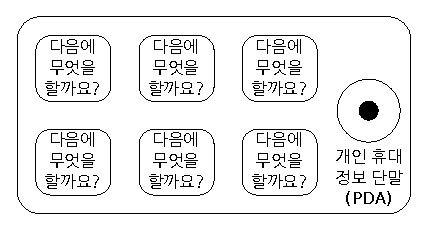
\includegraphics[height=1.00in]{figs2/pda2.eps}}
\afterfig

우선은 프로그래을 만드는 주된 동기가 사업을 위한다던가 사용자를 기쁘게 한다기 보다는 일상생활에서 맞닥드리는 자료와 정보를 잘 다뤄 좀더 생산적으로 우리의 삶을 만드는데 초점을 잡아보자. 프로그램을 만들기 시작할 때 여러분 모두는 프로그래머이면서 동시에 자신이 만든 프로그램의 사용자가 된다. 프로그래머로서 기술을 습득하고 프로그래밍 자체로 창의적으로 느껴진다면, 여러분은 다른 사람을 위해 프로그램을 개발하게 준비가 된 것이다.

\section{컴퓨터 하드웨어 아키텍처}
\index{hardware}
\index{hardware!architecture}

소프트웨어 개발을 위해 컴퓨터에 지시 명령어를 전달하기 위한 컴퓨터 언어를 배우기 전에, 컴퓨터가 어떻게 구성되어 있는지 이해할 필요가 있다. 컴퓨터 혹은 핸드폰을 분해해서 안쪽을 살펴보면, 다음의 주요 부품을 발견할 수 있다.

\beforefig
\centerline{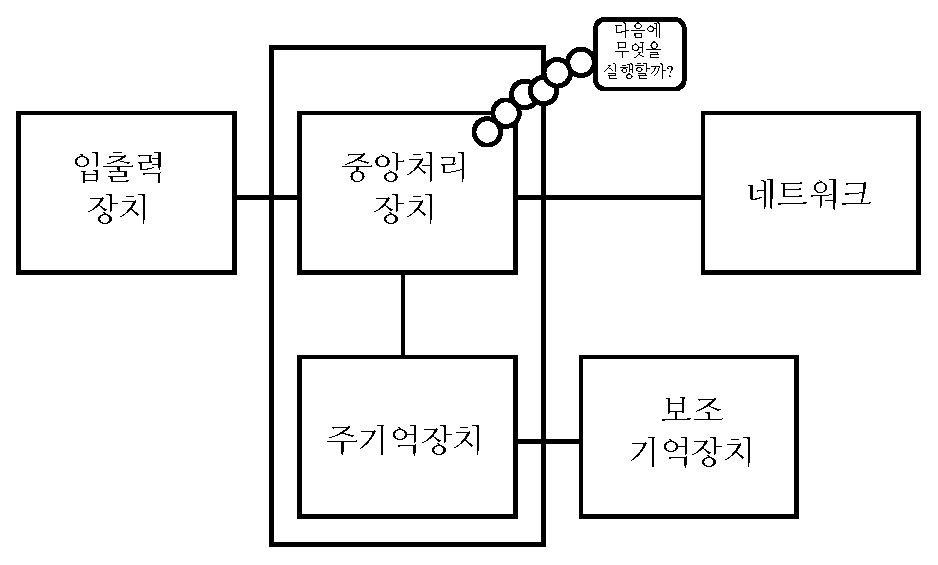
\includegraphics[height=2.50in]{figs2/arch.eps}}
\afterfig

주요 부품을 살펴보자.

\begin{itemize}

\item {\bf 중앙처리장치(Central Processing Unit, CPU): 다음은 무엇을 할까요? ("What is next?")} 명령어를 처리하는 주요 부분이다. 컴퓨터가 3.0 GHz라면 초당 명령어(다음은 무엇을 할까요? What is next?)를 삼백만번 처리할 수 있다고 계속 물을 수 있다. CPU의 처리속도를 따라서 컴퓨터와 빠르게 대화하는 것을 배울 것이다.

\item {\bf 주 기억장치(Main Memory):} 주기억장치는 중앙처리장치(CPU)가 급하게 명령어를 처리하기 위해 필요로 하는 정보를 저장하는 용도로 사용된다. 주 기억장치는 중앙처리장치만큼이나 빠르다. 그러나 주기억장치에 저장된 정보는 컴퓨터가 꺼지면 자동으로 지워진다.

\item[보조 기억장치] 보조 기억장치는 정보를 저장하기 위해 사용되지만, 주기억장치보다 속도가 느리다. 
전기가 나갔을 때도 정보를 기억하는 것이 장점이다. 휴대용 USB 기억장치나 이동 MP3 플레이어에 사용되는 USB의 플래쉬 메모리나 디스크 드라이브가 여기에 속한다.
 
\item {\bf 입출력장치(Input Output Devices):} 간단하게 화면, 키보드, 마우스, 마이크, 스피커, 터치패드가 포함된다. 컴퓨터와 사람이 상호작용하는 방식이다.

\item {\bf 네트워크(Network):} 요즘 거의 모든 컴퓨터는 네트워크로 정보를 주고 받는 네트쿼크 커넥션(Network Connection) 하드웨어를 가지고 있다. 네트워크는 정보를 저장하는 느린 저장소로 혹은 때때로 원하는 정보를 가져오지 못하는 것으로 보조 기억장치(Secondary memory)로 생각할 수 있다.

\end{itemize}
 

어떻게 이러한 주요 부품들이 작동하는지에 대한 자세한 사항은 컴퓨터를 만드는 사람에게 달려있지만, 프로그램을 만들때 컴퓨터 주요부품에 대해서 언급되어 컴퓨터 전문용어를 습득하고 이해하는 것은 도움이 된다.

프로그래머로서 여러분들은 사용자가 원하는 자료를 분석하고 문제를 풀 수 있는 컴퓨터 자원들을 사용하고 오케스트레이션하는 것이다.


\beforefig
\centerline{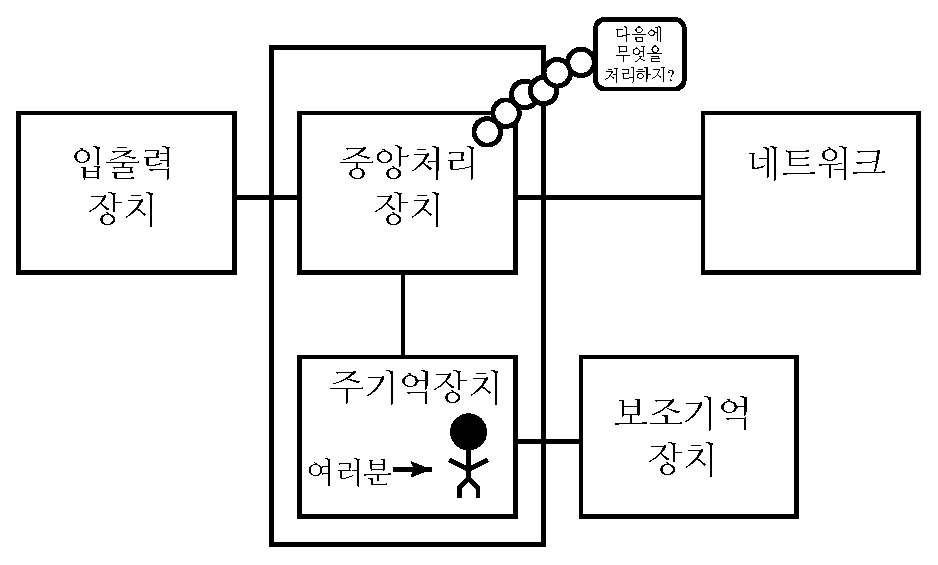
\includegraphics[height=2.50in]{figs2/arch2.eps}}
\afterfig

프로그래머로 중앙처리장치(CPU)와 대화하며 "다음은 무엇을 수행하세요"라고 지시할 것이다. 때때로 중앙처리장치(CPU)에게 주 기억장치, 보조 기억장치, 네트워크, 입출력 장치를 사용하라고 지시할 것이다.

프로그래머는 컴퓨터의 "다음은 무엇을 수행할까요"에 대한 답을 하는 사람이기도 하다. 하지만, 컴퓨터에 답하기 위해서 5mm 크기로 컴퓨터에 프로그래머를 집어넣고 초당 30억개의 명령어로 답을 하는 것은 매우 불편할 것이다. 그래서, 미리 컴퓨터에게 수행할 명령문을 써놔야한다. 이렇게 미리 작성된 명령문의 집합을 {\bf 프로그램(Program)}이라고 하며, 명령어 집합을 작성하고 명령어 집합이 올바르게 작성될 수 있도록 하는 행위를 {\bf 프로그래밍(Programming)}이라고 부른다.



\section{프로그래밍 이해하기}

책의 나머지 장을 통해서 책을 읽고 있는 당신을 프로그래밍의 장인으로 인도할 것입니다. 종국에는 책을 읽고 있는 여러분은 {\bf 프로그래머}가 될 것입니다. 아마도 전문적인 프로그러머는 아닐지라도 적어도 자료/정보 분석 문제를 보고 그 문제를 풀수 있는 기술을 가지게는 될 것입니다.

\index{problem solving}

이런 점에서 프로그래머가 되려면 두가지 기술이 필요로 합니다.

\begin{itemize}

\item 첫째, 파이썬같은 프로그래밍 언어 - 어휘와 문법을 알 필요가 있습니다. 단어를 새로운 언어에 맞추어 쓸 수 있어야 하며 새로운 언어를 잘 표현된 문장으로 구성하는지를 알아야 합니다.

\item 둘째, 스토리(Story)를 말 할 수 있어야 합니다. 스토리를 만들때, 독자에게 우리의 아이디어(idea)를 전달하기 위해서 단어와 문장을 조합합니다. 스토리를 만들 때 기술과 예술적인 면이 있으며, 기술과 예술적인 면은 여러번 쓰기 연습을 통하고 피트백을 받으므로써 향상됩니다. 프로그래밍에서, 우리가 만든 프로그램은 스토리이고, 풀려고 하는 문제는 "아이디어"에 해당합니다.

\end{itemize}

파이썬과 같은 프로그래밍 언어를 배우게 되면, 자바스크립트나 C++ 같은 두번째 언어를 배우는 것은 무척이나 쉽습니다. 새로운 프로그래밍 언어는 매우 다른 어휘와 문법을 가지지만, 문제푸는 기술을 배우기만 하면, 모든 프로그래밍 언어에서로 동일하게 접근할 수 있습니다.

파이썬의 어휘와 문단은 금방 배웁니다. 새로운 종류의 문제를 풀기위해 논리적인 프로그램을 짜는 것은 오래 걸립니다. 여러분은 작문을 배우듯이 프로그래밍을 배우게 될 것입니다. 프로그래밍을 읽고 설명하는 것으로 시작해서 간단한 프로그램을 작성하고, 점차적으로 복잡한 프로그램을 작성하게될 것입니다. 어느 순간에 명상에 잠기게 되고, 문제해결과 프로그램의 패턴을 보게되고, 좀더 자연스럽게 어떻게 문제를 받아들여 그 문제를 해결할 수 있는 프로그램을 작성하게 될 것입니다. 그리고, 그 순간에 도착하게 되면, 프로그래밍은 매우 즐겁고 창의적인 과정이 될 것입니다.

파이썬 프로그램의 어휘와 구조로 시작을 합니다. 간단한 예제가 언제 처음으로 프로그램을 읽기 시작했는지를 일깨워 주니 인내심을 가지세요.

\section{단어와 문장}
\index{programming language}
\index{language!programming}

사람의 언어와 달리, 파이썬의 어휘는 실질적으로 매우 적다. 어휘를 예약어(researved words)로 부른다. 이들 단어는 파이썬에 매우 특별한 의미를 가진다. 파이썬 프로그램에서 파이썬이 이들 단어를 보게되면, 이들 단어는 파이썬에게 단 하나의 유일한 의미를 지니게 된다. 후에 여러분들이 프로그램을 작성할 때 여러분들이 만든 자신만의 단어를 작성하게 되는데 이를 {\bf 변수(Variable)}라고 합니다. 여러분의 변수의 이름을 지을 때 폭넓은 자유를 가질 수 있지만, 변수의 이름으로 파이썬의 예약어를 사용할 수는 없습니다.

이런 점에서 강아지를 훈련시킬 때 "앉아", "기달려", 가져와 같은 특별한 어휘를 사용합니다. 강아지에게 이런 특별한 예약어를 사용하지 않을 때, 강아지는 주인이 특별한 어휘를 사용하지 않을 때 주인을 물끄러미 쳐다보기만 합니다. 예를 들어, "여러분이 더 많은 사람들이 건강을 전반적으로 향상하는 방향으로 가자 원한다"고 말하면, 강아지가 든는 것은 ''뭐라 뭐라 뭐라 {\bf walk} 뭐라'' 이렇게 들릴 것이다. 왜냐하면 "가자"가 강아지의 언어에는 예약어\footnote{\url{http://xkcd.com/231/}}이기 때문이다. 이러한 사실은 개와 사람사이에는 예약어가 없다는 것을 의미할지도 모른다.

사람이 파이썬에게 말을 하는 예약어는 다음과 같은 것이 있다.

\beforeverb
\begin{verbatim}
and       del       from      not       while    
as        elif      global    or        with     
assert    else      if        pass      yield    
break     except    import    print              
class     exec      in        raise              
continue  finally   is        return             
def       for       lambda    try
\end{verbatim}
\afterverb
%
강아지의 사례와는다르게 파이썬은 이미 완벽하게 훈련이 되어 있다. 여러분이 "try" 라고 말하면, 파이썬은 여러분이 매번 "try" 라고 말할 때마다 실패 없이 시도를 할 것이다.

이러한 예약어를 배울 것이고 어떻게 잘 사용되는지도 함께 배울것이지만, 지금은 파이썬에 말하는 것에 집중할 것이다. 파이썬에게 말하는 것 중 좋은 것은 다음과 같은 메세지를 던지는 것으로도 파이썬에 말을 할 수 있다는 것이다.

\beforeverb
\begin{verbatim}
print 'Hello world!'
\end{verbatim}
\afterverb

이 간단한 문장이 파이썬의 구문(Syntax)론적으로 완벽하다. 위 문장은 예약어 'print'로 시작해서 출력하고자 하는 문자열을 작은 따옴표로 감싸안아 올바르게 파이썬에게 전달했다.

\section{파이썬과 대화하기}

파이썬으로 우리가 알고 있는 단어를 가지고 간단한 문장을 만들었고, 새로운 언어 기술을 시험하기 위해서 파이썬과 대화를 어떻게 하는지 알 필요가 있다.

파이썬과 대화를 시작하기 전에, 파이썬 소프트웨어를 컴퓨터에 설치하고 컴퓨터에서 파이썬을 어떻게 실행하는지를 배워야 한다. 이번장에서 다루기에는 너무 구체적이고 자세한 사항이기 때문에 \url{www.pythonlearn.com}을 참조하는 것을 권고한다. 자세한 설치 방법과 화면을 캡쳐하여 윈도우와 매킨토쉬 시스템 및 실행하는 방법을 설명하였다. 설치가 마무리되고 터미널이나 명령어 실행창에서 {\bf python}을 치게되면 파이썬 인터프리터가 인터랙티브 모드로 실행을 시작하고 다음과 같은 것이 화면에 뿌려진다.

\index{interactive mode}

\beforeverb
\begin{verbatim}
Python 2.6.1 (r261:67515, Jun 24 2010, 21:47:49) 
[GCC 4.2.1 (Apple Inc. build 5646)] on darwin
Type "help", "copyright", "credits" or "license" for more information.
>>> 
\end{verbatim}
\afterverb
%
{\tt >>>} 프롬프트는 파이썬 인터프리터가 여러분에게 요청하는 방식이다. "다음에 파이썬이 무엇을 실행하기를 원합니까?" 파이썬은 여러분과 대화를 나눌 준비가 되었다. 이제 남은 것은 파이썬 언어로 어떻게 말하는 지를 여러분이 아는 것이고 여러분은 대화를 할 수 있다.

예를들어 여러분이 가장 간단한 파이썬 언어의 단어나 문장 조차도 알수가 없다고 가정해 봅시다. 우주 비행사가 저 멀리 떨어진 행성에 착륙할 때 사용하는 간단한 말을 사용하여 행성의 거주민에게 대화를 시도한다고 생각해 봅시다.

\beforeverb
\begin{verbatim}
>>> I come in peace, please take me to your leader
  File "<stdin>", line 1
    I come in peace, please take me to your leader
         ^
SyntaxError: invalid syntax
>>> 
\end{verbatim}
\afterverb
%
잘 되는것 같지 않습니다. 뭔가 빨리 다른 생각을 하지 않는다면, 행성의 거주민은 창으로 찔르고, 기름에 잘 발라 불위에서 바베큐를 만들어 저녁으로 먹을 듯 합니다.

운 좋게도 기나긴 우주 여행중 이책의 복사본을 가지고 와서 다음과 같이 빠르게 친다고 생각해봅시다.

\beforeverb
\begin{verbatim}
>>> print 'Hello world!'
Hello world!
\end{verbatim}
\afterverb
%

훨씬 좋아보기고, 좀더 커뮤니케이션을 이어갈 수 있을 것으로 보입니다.

\beforeverb
\begin{verbatim}
>>> print 'You must be the legendary god that comes from the sky'
You must be the legendary god that comes from the sky
>>> print 'We have been waiting for you for a long time'
We have been waiting for you for a long time
>>> print 'Our legend says you will be very tasty with mustard'
Our legend says you will be very tasty with mustard
>>> print 'We will have a feast tonight unless you say
  File "<stdin>", line 1
    print 'We will have a feast tonight unless you say
                                                     ^
SyntaxError: EOL while scanning string literal
>>> 
\end{verbatim}
\afterverb
%

이번 대화는 잠시동안 잘 진행되다가 여러분이 파이썬 언어로 말하다가 정말 사소한 실수를 저질러 파이썬이 오류를 뱉어낸다.

이번에 파이썬이 놀랍도록 복잡하고 강력하고 파이썬과 의사소통을 할때 사용하는 신택스(syntax)가 매우 까다롭다는 것은 알 수 있었다. 파이썬은 다른말로 똑똑(Intelligent)하지는 않다. 지금까지 여러분은 자신과 대화를 저절한 신택스(syntax)를 가지고 대화를 했습니다.

여러분이 다른사람이 작성한 프로그램을 사용한다는 것은 여러분과 파이썬을 사용하는 다른 프로그래머가 파이썬을 중간 매개체로 대화를 하는 것으로 볼 수 있습니다. 파이썬은 프로그램을 만든 저작자가 어떻게 대화가 진행되어져야 하는지를 표현하는 방식입니다. 다음 몇 장에 걸쳐서 여러분은 파이썬을 이용하여 여러분의 프로그램을 이용하는 다른 많은 프로그래머 중의 한명이 될 것입니다.

파이썬 인터프리터와 대화하는 첫 장을 끝내기 전에, 파이썬 행성의 거주자에게 "안녕히 계세요"를 말하는 적절한 방법을 알아야 한다.

\beforeverb
\begin{verbatim}
>>> good-bye
Traceback (most recent call last):
  File "<stdin>", line 1, in <module>
NameError: name 'good' is not defined

>>> if you don't mind, I need to leave
  File "<stdin>", line 1
    if you don't mind, I need to leave
             ^
SyntaxError: invalid syntax

>>> quit()
\end{verbatim}
\afterverb
%
위 처음 두개의 시도는 다른 오류 메세지를 출력한다. 두번째 오류는 다른데 이유는 {\bf if}가 예약어이기 때문에 파이썬은 이 예약어를 보고 뭔가 다른 것을 말한다고 생각하지만, 잠시 후 문장의 신택스가 잘못됐다고 판정하고 오류를 뱉어낸다.

파이썬에게 "안녕히 계세요"를 말하는 올바른 방식은 인터렉티브 {\tt >>>} 프롬프트에서 {\bf quit()}를 입력하는 것이다.



\section{전문용어: 인터프리터와 컴파일러}
파이썬은 사람이 읽고 쓸수 있고 컴퓨터도 읽고 쓸 수 있도록 고안된 {\bf 하이레벨(High-level)} 언어이다. 다른 하이레벨 언어는 자바, C++, PHP, 루비, 베이직, 펄, 자바스크립트 등 다수가 있다. 중앙처리장치(CPU)내에서 실제 하드웨어 수준에서 이런 하이레벨 언어를 이해하지 못한다.

중앙처리장치는 우리가 {\bf 기계어(machine-language)}로 부르는 언어만 이해한다. 기계어는 매우 간단하고 솔직히 작성하기에는 매우 지루하다. 왜냐하면 모두 0과 1로만 표현되기 때문이다.

\beforeverb
\begin{verbatim}
01010001110100100101010000001111
11100110000011101010010101101101
...
\end{verbatim}
\afterverb
%
0과 1로만 되어 있기 때문에 기계어가 간단해 보이지만, 시택스는 복잡하고 파이썬보다 훨씬 어렵다. 그래서 매우 소수의 프로그래머만이 기계어를 쓸수 있다. 대신에 파이썬과 자바스크립트 같은 하이레벨 언어로 프로그래머가 작성할 수 있도록 다양한 번역기(translator)를 만들었다. 이들 번역기는 프로그램을 중앙처리장치에 의해서 실제 실행이 가능한 기계어로 변환하여 준다.

기계어는 컴퓨터하드웨어에 묶여있기 때문에 기계어는 다른 형식의 하드웨어에 {\bf 이식(portable)}이 되지 않는다. 하이레벨 언어로 작성된 프로그램은 새로운 하드웨어위에 다른 인터프리터를 이용하여 옮겨 실행이 가능하고 다른 하드웨어에 사용할 수 있도록 프로그램을 다시 컴파일하여 사용할 수 있다.

프로그래밍 언어의 번역기는 두가지 범주가 있다. 
(1) 인터프리터 (2) 컴파일러

{\bf 인터프리터}는 프로그래머에 의해서 쓰여진 소스코드를 읽고, 소스코드를 파싱하고, 즉석에서 명령어를 해석한다. 파이썬은 인터프리터다. 파이썬을 인터렉트브 모드로 실행할때, 파이썬 명령문을 쓰면, 파이썬이 즉성에서 처리하고, 다른 파이썬 명령어를 여러분으로부터 기다린다.

파이썬 명령어는 파이썬이 나중에 사용될 값을 기억하기를 바란다. 적당한 이름을 잡아서 그 값을 기억시키고, 나중에 그 이름을 호출하여 값을 사용할 수 있다. 이러한 목적으로 값을 저장하는 것을 {\bf 변수(variable)}라고 한다.

\beforeverb
\begin{verbatim}
>>> x = 6
>>> print x
6
>>> y = x * 7
>>> print y
42
>>> 
\end{verbatim}
\afterverb
%
이 예제에서 파이썬이 x라는 라벨을 사용하여 6이라는 값을 저장하기를 바라고 나중에 사용코저 한다. {\bf print} 예약어를 사용하여 파이썬이 잘 기억하고 있는지를 검증한다. 그리고 {\bf x}를 반환하여 7을 곱하고 새로운 변수 {\bf y}에 값을 집어 넣는다. 그리고 {\bf y}에 현재 무엇이 저장되어 있는지 출력하라고 파이썬에게 요청한다.

파이썬에 한줄 한줄 명령어를 쳐 넣고 있지만, 파이썬은 앞쪽에 명령문에서 생성된 자료가 나중의 실행 명령문에서 사용될 수 있도록 정렬된 명령문으로 처리한다. 방금전 논리적이고 의미있는 순서로 4줄의 명령문을 가진 한 단락을 작성한 것이다.

위에서 본것처럼 파이썬과 대화를 주고받을 수 있는 것이 {\bf 인터프리터}의 본질이다. {\bf 컴파일러}는 완전한 프로그램을 하나의 파일에 담겨지고, 하이레벨 소스코드가 기계어로 번역되고, 컴파일러가 나중에 실행되도록 기계어를 파일에 담아놓는다.

윈도우를 사용한다면, 실행가능한 기계어 프로그램의 확장자가 ".exe"(executable), 혹은 ".dll"(dynamically loadable library)임을 확인할 수 있다. 리눅스와 매키토쉬에서는 실행화일을 의미하는 확장자는 없다.

텍스트 편집기에서 실행파일을 열게되면 다음과 같은 읽을 수 없는 좀 괴상한 출력을 화면상에서 확인할 수 있다.

\beforeverb
\begin{verbatim}
^?ELF^A^A^A^@^@^@^@^@^@^@^@^@^B^@^C^@^A^@^@^@\xa0\x82
^D^H4^@^@^@\x90^]^@^@^@^@^@^@4^@ ^@^G^@(^@$^@!^@^F^@
^@^@4^@^@^@4\x80^D^H4\x80^D^H\xe0^@^@^@\xe0^@^@^@^E
^@^@^@^D^@^@^@^C^@^@^@^T^A^@^@^T\x81^D^H^T\x81^D^H^S
^@^@^@^S^@^@^@^D^@^@^@^A^@^@^@^A\^D^HQVhT\x83^D^H\xe8
....
\end{verbatim}
\afterverb
%
It is not easy to read or write machine language so it is nice that we have
{\bf interpreters} and {\bf compilers} that allow us to write in a high-level
language like Python or C.

Now at this point in our discussion of compilers and interpreters, you should 
be wondering a bit about the Python interpreter itself.  What language is 
it written in?  Is it written in a compiled language?  When we type
``python'', what exactly is happening?

The Python interpreter is written in a high level language called ``C''.  
You can look at the actual source code for the Python interpreter by
going to \url{www.python.org} and working your way to their source code.
So Python is a program itself and it is compiled into machine code and
when you installed Python on your computer (or the vendor installed it),
you copied a machine-code copy of the translated Python program onto your
system.   In Windows the executable machine code for Python itself is likely
in a file with a name like:

\beforeverb
\begin{verbatim}
C:\Python27\python.exe
\end{verbatim}
\afterverb
%
That is more than you really need to know to be a Python programmer, but
sometimes it pays to answer those little nagging questions right at 
the beginning.

\section{프로그램 작성하기}

파이썬 인터프리터에 명령어를 치는 것은 파이썬의 주요기능을 알아볼 수 있는 좋은 방법이지만 좀더 복잡한 문제를 해결하기 위해서는 권해드리지는 않습니다.

프로그램을 작성할 때 {\bf 스크립트(script)}로 불리는 파일에 명령어 집합을 작성하기 위해서 텍스트 편집기를 주로 사용합니다. 파이썬 스크립트는 {\tt .py}라는 확장자를 가집니다.

\index{script}

스크립트를 실행하기 위해서 파이썬 인터프리터에게 파일의 이름을 말해줍니다. 유니스나 윈도우 명령창에서 {\tt python hello.py}를 치게 되면 다음과 같은 결과를 얻게 됩니다.

\beforeverb
\begin{verbatim}
csev$ cat hello.py
print 'Hello world!'
csev$ python hello.py
Hello world!
csev$
\end{verbatim}
\afterverb
%
''csev\$''은 운영시스템의 명령어 프롬프트이고, ''cat hello.py''는 문자열을 출력하라는 한줄의 파이썬 프로그램을 표시하라는 명령어입니다.

인터랙트브 모드로 파이썬 코드를 보여달라는 방식 대신에 파이썬 인터프리터를 호출하고 ''hello.py'' 파일에서 소스코드를 읽으라고 말하는 것입니다.

이 새로운 방식은 파이썬 프로그램을 끝내기 위해 {\bf quit()}를 사용할 필요가 없는 것이 좋은 점입니다. 파이썬이 파일에서 소스코드를 읽을 때, 파일 끝까지 읽게되면 파이썬은 자동으로 끝낼 줄을 알고 있습니다.

\section{프로그램이란 무엇인가?}

{\bf 프로그램(Program)}의 가장 기본적인 정의는 어떠한 일을 할 수 있도록 조작된 일련의 파이썬 명령문의 집합이다. 가장 간단한 {\bf hello.py} 스크립트도 프로그램이다. 한줄의 프로그램으로 특별히 유익하고 쓸모가 있는 것은 아니지만 엄격한 의미에서 파이썬 프로그램이 맞다.

프로그램을 이해하는 가장 쉬운 방법은 프로그램이 어떠한 문제를 풀려고 만들어졌는지 문제를 먼저 생각하는 것이다. 그리고 그 문제를 풀려고 작성된 프로그램을 살펴보는 것이다.

예를 들어 여러분이 페이스북의 일련의 게시된 글에 가장 자주 사용된 단어에 관심을 가지고 소셜 컴퓨팅 연구를 한다고 생각해 봅시다. 페이스북에 게시된 글들을 출력하고 가장 흔한 단어를 찾으로 열심히 들여다 볼 것이지만 매우 오래걸리고 실수하기 쉽습니다. 하지만 파이썬 프로그램을 이용하면, 빨리 정확하게 작업을 할 수 있는 파이썬 프로그램을 작성해서 주말에 뭔가 재미있는 일로 보낼 수 있습니다.

예를 들어 다음의 자동차(car)와 광대(clown)를 보고, 가장 많이 나오는 단어는 무엇이며 몇번 나왔는지 세어보세요.

\beforeverb
\begin{verbatim}
the clown ran after the car and the car ran into the tent 
and the tent fell down on the clown and the car 
\end{verbatim}
\afterverb
%

그리고, 몇백만줄의 텍스트를 보고서 동일한 일을 한다고 상상해 보세요. 솔직히 수작업으로 단어를 세는 것보다 파이썬을 배워 프로그램을 배우는 것이 훨씬 빠를 것입니다.

더 좋은 소식은 이미 텍스트 파일에서 가장 자주 나오는 단어를 찾아내는 간단한 프로그램을 제시했고, 작성했고, 시험까지 했다. 이걸 가지고 여러분들은 바로 사용을 할 수 있기 때문에 수고를 덜 수 있다.

\beforeverb
\begin{verbatim}
name = raw_input('Enter file:')
handle = open(name, 'r')
text = handle.read()
words = text.split()
counts = dict()

for word in words:
   counts[word] = counts.get(word,0) + 1

bigcount = None
bigword = None
for word,count in counts.items():
    if bigcount is None or count > bigcount:
        bigword = word
        bigcount = count

print bigword, bigcount
\end{verbatim}
\afterverb
%
이 프로그램을 사용하려고 파이썬을 알 필요도 없다. 10장에 걸쳐서 멋진 파이썬 프로그램을 만드는 방법을 배우게 될 것입니다. 지금 여러분은 사용자로 단순히 프로그램을 사용하지만 이 프로그램이 얼마나 많은 수작업을 줄일 수 있는지 보여주고 있다. 코드를 작성하고 {\bf words.py}로 저장하여 실행을 하거나, \url{http://www.pythonlearn.com/code/}에서 소스코드를 다운로드 받아 실행하면 된다.

\index{program}
파이썬과 파이썬 언어가 중간의 중개자로서 여러분(사용자)과 저자(프로그래머)사이에서 중개자의 역할을 훌륭히 하고 있는 것을 보여주고 있습니다. 파이썬이 설치된 컴퓨터에서 누구나 사용할 수 있는 공통의 언어로 유용한 명령 순서(즉, 프로그램)를 주고받는지 보여준다. 그래서 {\em 파이썬과} 직접의사소통하지 않고 {\em 파이썬을 통해서} 서로 의사소통할 수 있다.

\section{프로그램 구성요소}

다음의 몇장에 걸쳐서 파이썬 어휘, 문장구조, 문단구조에 대해서 배울 것이다. 파이썬의 강력한 점에 대해서 배울 것이고, 유용한 프로그램을 작성하기 위해서 파이썬의 역량을 조합하는 법을 배울 것이다.

프로그램을 작성하기 위해서 사용하는 로우레벨(low-level) 패턴이 몇가지 있다. 파이썬을 위해서 만들어졌다기 보다는 기계어부터 하이레벨 언어에 이르기까지 모든 언어에 공통된 사항이다.

\begin{description}

\item[입력:] 컴퓨터 바깥세계에서 데이터를 가져온다. 파일로부터 데이터를 읽을 수도 있고, 마이크나 GPS 같은 센서에서 데이터를 입력받을 수도 있다. 위 프로그램에서 사용자의 키보드로 데이터를 입력받아 입력값으로 사용된 사례이다.

\item[출력:] 화면에 프로그램의 결과값을 보여주거나 파일에 저장한다. 혹은 음악을 연주하거나 텍스트를 읽도록 스피커 같은 장치에 데이터를 보낸다.

\item[순차 실행:] 스크립트에 작성된 순서에 맞추어 한줄 한줄 실행된다.

\item[조건 실행:] 조건을 확인하고 명령문을 실행하거나 건너뛴다.

\item[반복 실행:] 반복적으로 명령문을 실행한다. 대체로 반복 실행시 변화를 수반한다.

\item[재사용:] 명령어를 한번 작성하고 이름을 주어 저장하고 프로그램의 필요에 따라 이름을 불러 몇차례 다시 사용한다.

\end{description}

너무나 간단하게 들리지만, 전혀 간단하지는 않다. 걸음거리를 간단히 ''한 다리를 다를 다리 앞에 놓으세요'' 라고 말하는 것 같다. 프로그램을 짜는 ''예술''은 이러한 기본 요소를 조합하고 엮어 사용자에게 유용한 무언가를 만드는 것이다.

단어를 세는 프로그램은 위 프로그램의 기본요소를 하나만 빼고 모두 사용하여 작성되었다.


\section{프로그램이 잘못되면?}

파이썬과 처음에 대화를 할때, 파이썬 코드를 명확하게 작성하여 의사소통을 해야한다. 작은 차이 혹은 실수는 파이썬이 여러분이 작성한 프로그램을 보다가 포기하게 만듭니다.

초보 파이썬 프로그래머는 파이썬이 오류에 대해서는 인정사정볼 것 없다고 생각합니다. 파이썬이 모든 사람을 좋아하는 것 같지만, 파이썬은 사적으로 사람들을 알고 있고, 뒤끝이 있습니다. 이러한 사실로 인해서 파이썬은 완벽하게 작성된 프로그램만을 가지게 되고 ''잘못 작성되었어요''라고 뱉어내고 여러분에게 고통을 줍니다.

\beforeverb
\begin{verbatim}
>>> primt 'Hello world!'
  File "<stdin>", line 1
    primt 'Hello world!'
                       ^
SyntaxError: invalid syntax
>>> primt 'Hello world'
  File "<stdin>", line 1
    primt 'Hello world'
                      ^
SyntaxError: invalid syntax
>>> I hate you Python!
  File "<stdin>", line 1
    I hate you Python!
         ^
SyntaxError: invalid syntax
>>> if you come out of there, I would teach you a lesson
  File "<stdin>", line 1
    if you come out of there, I would teach you a lesson
              ^
SyntaxError: invalid syntax
>>> 
\end{verbatim}
\afterverb
%

파이썬과 다퉈봐야 얻을 것은 없어요. 파이썬은 도구고 감정이 없습니다. 여러분이 필요로 할 때마다 여러분에게 봉사하고 기쁨을 주기 위해서 존재할 뿐입니다. 오류 메세지가 심하게 들릴지는 모르지만 단지 파이썬이 도와달라고 하는 요청일 뿐입니다. 여러분이 입력한 것을 쭉 읽어보고 여러분이 입력한 것을 이해할 수 없다고만 말할 뿐입니다.

파이썬은 어떤면에서 강아지와 닮았습니다. 맹목적으로 여러분을 사랑하고, 강아지가 이해하는 몇몇 단어만 이해하며, 웃는 표정({\tt >>>} 명령 프롬프트)으로 여러분이 무언가를 말하기만을 기다립니다. 파이썬이 ''SyntaxError: invalid syntax''을 뱉어낼 때, 꼬리를 흔들면서 ''뭔가 말씀하시는 것 같은데요... 주인님 말씀을 이해하지 못하겠어요, 다시 말씀해 주세요 ({\tt >>>})'' 말하는 것과 같다.

여러분이 작성하는 프로그램이 점점 유용해지고 복잡해짐에 따라 3가지 유형의 오류를 마주치게 된다.

\begin{description}

\item[구문 오류(Syntax Error):]첫번째 마주치는 오류로 고치기 가장 쉽습니다. 구문 오류는 파이썬의 문법에 맞지 않는다는 것을 의미합니다. 파이썬은 구문오류가 발생한 줄을 찾아 정확한 위치를 알려줍니다. 하지만, 파이썬이 제시하는 오류가 그 이전 프로그램 부문에서 발생했을 수도 있기 때문에 파이썬이 알려주는 곳 뿐만 아니라 그 앞쪽도 살펴볼 필요가 있다. 따라서 파이썬이 제시하는 구문 오류의 경우 오류가 난 곳은 오류를 고치기 위한 시작점으로 의미가 있다.

\item[논리 오류(Logic Error):] 논리 오류는 프로그램의 구문은 완벽하지만 명령문의 실행에 혹은 다른 명령어부분과 관련된 부문에서 실수가 있는 것이다. 논리 오류의 예를 들어보자. ''물병에서 한모금 마시고, 가방에 넣고, 도서관으로 걸어가서, 물병을 닫는다''

\item[시맨틱 오류(Semantic Error):] 시맨틱 오류는 구문론적으로 완벽하고 올바른 순서로 프로그램의 명령문이 작성되었지만 프로그램에 오류가 숨어있다. 프로그램은 완벽하게 작동하지만 여러분이 의도한 바를 수행하지는 못합니다. 간단한 예로 여러분이 식당으로 가는 방향을 알려주고 있습니다. '' ... 주유소 사거리에 도착했을 때, 왼쪽으로 돌아 1.6km 쭉 가면 왼쪽편에 빨간색 빌딩에 식당이 있습니다.'' 친구가 매우 늦어 전화로 지금 농장에 있고 헛간으로 걸어가고 있는데 식당을 발견할 수 없다고 전화를 합니다. 그러면 여러분은 ''주유소 왼쪽 혹은 오른쪽을 돈거야'' 말하면, 그 친구는 ''말한대로 완벽하게 따라서 했고, 말한대로 적기까지 했는데, 왼쪽으로 돌아 1.6km에 주요소가 있다고 했어'', 그러면 여러분은 ''미안해, 내가 가지고 있는 건 구문론적으로는 완벽한데, 사소한 시맨틱 오류가 있네!'' 라고 말할 것이다.

\end{description}

위 세 종류의 오류에 대해서 파이썬은 여러분이 요청한 것을 충실히 수행하기 위해서 최선을 다합니다.

\section{학습으로의 여정}

여러분이 책을 읽으면서 개념들이 처음에 잘 와 닿지 않는다고 기죽을 필요는 없어요. 여럽누이 말하는 것을 배울 때, 처음 몇년동안 웅얼거리는 것은 문제가 아닙니다. 간단한 어휘에서 간단한 문장으로 옮겨가고, 문장에서 문단으로 옮겨가는데 6개월이 걸려도 괜찮습니다. 흥미로운 완벽한 짧은 스토리를 자신의 언어로 작성하는데 몇 년이 걸립니다.

여러분이 파이썬을 빨리 배울수 있도록 다음의 몇장에 걸쳐서 정보를 제공해 드릴 것입니다. 새로운 언어를 습득하는 것과 같아서 자연스럽게 느껴지기까지 흡수하고 이해하기까지 시간이 걸립니다. 큰 그림(Big Picture)을 이루는 작은 조각을 정의하면서 여러분을 큰 그림을 볼 수 있도록 여러 주제를 찾고, 또 찾으면서 혼란이 생길 수 있다. 이책이 순차 선형적으로 쓰여져서 본 과정을 선형적으로 배워갈 수도 있지만, 비선형적으로 본 교재를 활용하는 것도 괜찮다. 가볍게 앞쪽과 뒷쪽을 넘나들며 책을 읽을 수도 있다. 구체적이고 세세한 점을 완벽하게 이해하지 않고 고급 과정을 가볍게 읽으면서 프로그래밍의 ''왜(Why)''에 대해서 더 잘 이해할 수도 있다. 앞에서 배운것을 다시 리뷰하고 앞의 연습문제를 다시 하면서 처음에 난공불락이라 여겼던 어려운 주제도 더잘 배우고 이해할 수 있다는 것을 알게될 것이다.

대체적으로 처음 프로그래밍 언어를 배울 때 망치로 돌을 내리치고, 끌로 깎아내고 하면서 아름다운 조각품을 만들면서 겪게되는 몇 번의 '' 유레카, 아 하~~'' 순간이 있다.

만약 어떤 것이 특별히 힘들다면, 밤새도록 앉아서 지켜보고 노력하는 것은 별로 의미가 없다. 잠시 쉬고, 낮잠을 자고, 간식을 먹고 다른사람이나 강아지에게 문제를 설명하고 자문을 구한 후에 깨끗한 정신과 눈으로 돌아와서 다시 시도해보라. 단언컨데 이책의 프로그래밍 개념을 배우자마자 정말 쉽고 멋지다는 것을 돌이켜 보면 알게될 것이다. 프로그래밍 언어는 정말 배울 가치가 있다.

\section{용어사전}

\begin{description}

\item[버그(bug):]  프로그램 오류
\index{bug}

\item[중앙처리장치(central processing unit, CPU):] 컴퓨터의 심장, 여러분이 작성한 프로그램을 실행하는 장치, "CPU" 혹은 프로세서라고 불립니다.
\index{central processing unit}
\index{CPU}

\item[컴파일러(compile):]  하이레벨 언어로 작성된 프로그램을 로우레벨 언어로 즉시 혹은 나중에 사용하도록 번역하는 번역기
\index{compile}

\item[하이레벨 언어(high-level language):]  사람이 읽고 쓰기 쉽게 설계된 파이썬과 같은 프로그래밍 언어
\index{high-level language}

\item[인터랙티브 모드(interactive mode):] 프롬프트에서 명령어나 표현식을 입력함으로써 파이썬 인터프리터를 사용하는 방식
\index{interactive mode}

\item[인터프리트(interpret):] 하이레벨 언어의 프로그램을 한번에 한줄씩 번형해서 실행하는 것
\index{interpret}

\item[로우레벨 언어(low-level language):] 컴퓨터가 실행하기 쉽게 설계된 프로그래밍 언어, ''기계어 코드'', ''어셈블리 언어''로 불린다.
\index{low-level language}

\item[기계어 코드(machine code):] 중앙처리장치에 의해서 바로 실행될수 있는 가장 낮은 수준의 언어로된 소프트웨어
\index{machine code}

\item[주메모리(main memory):] 프로그램과 데이터를 저장한다. 전기가 나가게 되면 주메모리에 저장된 정보는 사라진다.
\index{main memory}

\item[파싱(parse):]  프로그램을 검사하고 구문론적 구조를 분석하는 것
\index{parse}

\item[이식(portability):] 하나 이상의 컴퓨터에서 실행될 수 있는 프로그램의 특성
\index{portability}

\item[출력문(print statement):] 파이썬 인터프리터가 화면에 값을 출력할 수 있게 만드는 명령문
\index{print statement}
\index{statement!print}

\item[문제해결(problem solving:)] 문제를 만들고, 답을 찾고, 답을 표현하는 과정
\index{problem solving}

\item[프로그램(program:)] 컴퓨테이션(Computation)을 명세하는 명령어의 집합
\index{program}

\item[프롬프트(prompt):] 프로그램이 메세지를 출력하고 사용자가 프로그램에 입력하도록 기다릴 때.
\index{prompt}

\item[보조 기억장치] 전기가 나갔을 때도 정보를 기억하고 프로그램을 저장하는 저장소. 일반적으로 주메모리보다 속도가 느리다. USB의 플래쉬 메모리나 디스크 드라이브가 여기에 속한다.
\index{secondary memory}

\item[시맨틱(semantics):]  프로그램의 의미
\index{semantics}

\item[시맨틱 오류(semantic error):]  프로그래머가 의도한 것과 다른 행동을 하는 프로그램의 오류
\index{semantic error}

\item[소스코드(source code):]  하이레벨 언어로 기술된 프로그램
\index{source code}

\end{description}

\section{연습문}


\begin{ex}
컴퓨터 보조기억장치의 기능은 무엇입니까?

a) 모든 연산과 프로그램의 로직을 수행한다.\\
b) 인터넷의 웹페이지를 불러온다.\\
c) 파워가 없을 때도 장시간 정보를 저장한다.\\
d) 사용자로부터 입력정보를 받는다.
\end{ex}

\begin{ex}
프로그램은 무엇입니까?
\end{ex}

\begin{ex}
컴파일러와 인터프리터의 차이점을 설명하세요.
\end{ex}

\begin{ex}
기계어 코드는 다음중 어는 것입니까?

a) 파이썬 인터프리터\\
b) 키보드\\
c) 파이썬 소스코드 파일\\
d) 워드 프로세싱 문서
\end{ex}

\begin{ex}
 다음 코드에서 잘못된 점을 설명하세요.

\beforeverb
\begin{verbatim}
>>> primt 'Hello world!'
  File "<stdin>", line 1
    primt 'Hello world!'
                       ^
SyntaxError: invalid syntax
>>> 
\end{verbatim}
\afterverb

\end{ex}

\begin{ex}
다음의 파이썬 프로그램이 실행된 후에 변수 "X"는 어디에 저장됩니까?

\beforeverb
\begin{verbatim}
x = 123
\end{verbatim}
\afterverb
%
a) 중앙처리장치\\
b) 주메모리\\
c) 보조메모리\\
d) 입력장치\\
e) 출력장치
\end{ex}

\begin{ex}
다음 프로그램에서 출력되는 것은 무엇입니까?

\beforeverb
\begin{verbatim}
x = 43
x = x + 1
print x
\end{verbatim}
\afterverb
%
a) 43\\
b) 44\\
c) x + 1\\
d) 오류, 왜냐하면 x = x + 1 은 수학적으로 불가능하다.
\end{ex}

\begin{ex}
사람의 어느 능력부위에 해당하는지 예로하여 다음을 설명하세요.
(1) 중앙처리장치, (2) 주메모리, (3) 보조메모리, 
(4) 입력장치
(5) 출력장치
중앙처리장치에 상응하는 사람의 몸 부위는 어디입니까? 
\end{ex}

\begin{ex}
구문오류("Syntax Error")는 어떻게 고칩니까?
\end{ex}


%% LaTeX source for ``Python for Informatics: Exploring Information''
% Copyright (c)  2010-  Charles R. Severance, All Rights Reserved

\chapter{변수, 표현식, 스테이트먼트(Statement)}

\section{값(Value)과 형(Type)}
\index{값(value)}
\index{형(type)}
\index{문자열(string)}

{\bf 값(Value)}은 문자와 숫자처럼 프로그램이 다루는 가장 기본이 되는 단위이다. 
지금까지 살펴본 값은 {\tt 1}, {\tt 2} 그리고 \verb"'Hello,World!'" 이다.

상기 값은 다른 {\bf 형(Type)}에 속하는데, {\tt 2}는 정수, \verb" 'Hello,World!'" 는 
{\bf 문자열(String)}에 속하는데, 문자(Letter)를 일련의 열(sequence)의 형태로 되어 있어서 문자열이라고 부른다. 
인용부호에 감싸여 있어서, 여러분과 인터프리터는 문자열을 식별할 수 있다. 

{\tt print } 문은 정수에도 사용할 수 있다. {\tt python} 명령어를 실행하여 인터프리터를 구동시키자.

\index{quotation mark}

\beforeverb
\begin{verbatim}
python
>>> print 4
4
\end{verbatim}
\afterverb
%
값이 어떤 형인지 확신을 못한다면, 인터프리터가 알려준다.

\beforeverb
\begin{verbatim}
>>> type('Hello, World!')
<type 'str'>
>>> type(17)
<type 'int'>
\end{verbatim}
\afterverb
%

놀랍지도 않게, strings은 {\tt str} 형식이고, 정수는 {\tt int} 형식이다. 
다소 명백하지는 않지만, 소숫점을 가진 숫자는 {\tt float} 형식이다. 왜냐하면 이들 숫자가 {\bf 부동소수점} 형식으로 표현되기 때문이다.

\index{형(type)}
\index{문자열형}
\index{형(type)!문자열형}
\index{정수형}
\index{형(type)!정수형}
\index{부동소수점형}
\index{형(type)!부동소수점형}

\beforeverb
\begin{verbatim}
>>> type(3.2)
<type 'float'>
\end{verbatim}
\afterverb
%

\verb"'17'", \verb"'3.2'" 같은 값은 어떨가? 숫자처럼 보이지만 문자열처럼 인용부호에 감싸여 있다.

\index{quotation mark}

\beforeverb
\begin{verbatim}
>>> type('17')
<type 'str'>
>>> type('3.2')
<type 'str'>
\end{verbatim}
\afterverb
%

\verb"'17'", \verb"'3.2'" 은 문자열이다.

{\tt 1,000,000} 처럼 아주 큰 정수를 입력할 때, 세자리 숫자마다 콤마(,)를 사용하고 싶을 것이다. 하지만, 파이썬에서 적법하게 정수를 표현하는 것은 아니지만 문법적으로는 적합하다.

\beforeverb
\begin{verbatim}
>>> print 1,000,000
1 0 0
\end{verbatim}
\afterverb
%

하지만, 파이썬 실행 결과는 우리가 기대했던 것이 아니다. 파이썬에서는 {\tt 1,000,000} 을 콤마(',')로 구분된 정수로 인식한다. 따라서 사이 사이 공백을 넣어 출력했다.

\index{의미론적 오류} % \index{semantic error}
\index{오류!의미론} % \index{error!semantic}
\index{오류 메시지}

이 사례가 여러분이 처음 경험하게 되는 의미론적 오류(semantic error)다. 
코드가 에러 메세지 없이 실행이되지만, ''올바른(right)'' 작동을 하는 것은 아니다.

\section{변수(Variable)}
\index{변수} % \index{variable}
\index{할당문} %\index{assignment statement}
\index{문장!할당문} % \index{statement!assignment}

프로그래밍 언어의 가장 강력한 기능 중의 하나는 변수를 다룰 수 있는 능력이다. {\bf 변수(Variable)}는 값을 참조하는 이름이다.

{\bf 할당문(Assignment statement)}는 새로운 변수를 생성하고 값을 변수에 할당한다.

\beforeverb
\begin{verbatim}
>>> message = 'And now for something completely different'
>>> n = 17
>>> pi = 3.1415926535897931
\end{verbatim}
\afterverb
%

상기 예제는 세가지 할당사례를 보여준다. 첫 번째 할당 예제는 {\tt message} 변수에 문자열을 할당한다. 두 번째 예제는 변수 {\tt n}에 정수 {\tt 17}을 할당한다. 세 번째 예제는 {\tt pi}변수에 $\pi$ 근사값을 할당한다.

변수 값을 출력하기 위해서 {\tt print}문을 사용한다.

\beforeverb
\begin{verbatim}
>>> print n
17
>>> print pi
3.14159265359
\end{verbatim}
\afterverb
%

변수의 형(type)은 변수가 참조하는 값의 형이다.

\beforeverb
\begin{verbatim}
>>> type(message)
<type 'str'>
>>> type(n)
<type 'int'>
>>> type(pi)
<type 'float'>
\end{verbatim}
\afterverb
%

\section{변수명(Variable name)과 예약어(keywords)}
\index{예약어} % \index{keyword}

대체로 프로그래머는 의미있는 변수명을 고른다. 프로그래머는 변수가 사용되는 것에 대해 문서화도 한다.

변수명은 임의로 길 수 있다. 변수명은 문자와 숫자를 포함할 수 있지만, 문자로 변수명을 시작해야 한다. 첫 변수명을 대문자로 사용해도 되지만 소문자로 변수명을 시작하는 것도 좋은 생각이다. (후에 왜 그런지 보게 될 것이다.)

변수명에 밑줄(underscore character, \verb"_")이 들어갈 수 있다. 종종 \verb"my_name" 혹은 \verb"airspeed_of_unladen_swallow" 처럼 밑줄은 여러 단어와 함께 사용된다.
변수명을 밑줄로 시작해서 작성할 수 있지만, 다른 사용자가 사용할 라이브러리를 작성하는 경우가 아니라면, 일반적으로 밑줄로 시작하는 변수명은 피한다.

\index{밑줄} % \index{underscore character}

변수명을 적합하게 작성하지 못하다면, 구문 오류가 발생한다.

\beforeverb
\begin{verbatim}
>>> 76trombones = 'big parade'
SyntaxError: invalid syntax
>>> more@ = 1000000
SyntaxError: invalid syntax
>>> class = 'Advanced Theoretical Zymurgy'
SyntaxError: invalid syntax
\end{verbatim}
\afterverb
%

{\tt 76trombones} 변수명은 문자로 시작하지 않아서 적합하지 않다. 
{\tt more@}은 특수 문자 ({\tt @})를 변수명에 포함해서 적합하지 않다. 
하지만, {\tt class} 변수명은 뭐가 잘못된 것일까?

구문 오류 이유는 {\tt class}가 파이썬의 예약어 중의 하나라고 밝혀졌다. 
인터프리터가 예약어를 사용하여 프로그램 구조를 파악하기 위해서 사용하지만, 변수명으로는 사용할 수 없다.

\index{예약어}
%\index{keyword}

파이썬에는 31개 키워드\footnote{Python 3.0 에서 {\tt exec} 은 더 이상 예약어가 아니지만, {\tt nonlocal} 은 여전히 예약어다.}가 예약어로 이미 사용중에 있다.

\beforeverb
\begin{verbatim}
and       del       from      not       while    
as        elif      global    or        with     
assert    else      if        pass      yield    
break     except    import    print              
class     exec      in        raise              
continue  finally   is        return             
def       for       lambda    try
\end{verbatim}
\afterverb
%

상기 예약어 목록을 주머니에 넣고 잘 가지고 다니고 싶을 것이다. 
만약 인터프리터가 변수명 중 하나에 대해 불평을 하지만 이유를 모르는 경우, 예약어 목록에 변수명이 있는지 확인해 보세요.

\section{문장(Statement)}

{\bf 문장(statement)}은 파이썬 인터프리터가 실행하는 코드 단위다. 지금까지 print, assignment 두 종류의 문장을 살펴봤습니다.

\index{문장}
\index{인터랙티브 모드}
\index{스크립트 모드}
%\index{statement}
%\index{interactive mode}
%\index{script mode}

인터랙트브 모드에서 문장을 입력하면, 인터프리터는 문장을 실행하고, 만약 출력할 것이 있다면 결과를 화면에 출력합니다.

스크립트는 보통 여러줄의 문장으로 구성됩니다. 하나 이상의 문장이 있다면, 스트테이트먼트가 실행되며서 결과가 한번에 하나씩 나타납니다.

예를 들어, 다음의 스크립트를 생각해 봅시다.

\beforeverb
\begin{verbatim}
print 1
x = 2
print x
\end{verbatim}
\afterverb
%

상기 스크립트는 다음 결과를 출력합니다.

\beforeverb
\begin{verbatim}
1
2
\end{verbatim}
\afterverb
%

할당 문장{\tt (x=2)}은 결과를 출력하지 않습니다.

\section{연산자(Operator)와 피연산자(Operands)}
\index{연산자, 산술}
\index{산술 연산자}
\index{피연산자}
\index{표현식}

%\index{operator, arithmetic}
%\index{arithmetic operator}
%\index{operand}
%\index{expression}

{\bf 연산자(Operators)}는 덧셈, 곱셈 같은 계산(Computation)을 표현하는 특별한 기호입니다. 연산가자 적용되는 값을 {\bf 피연산자(operands)}라고 합니다.

다음의 예제에서 보듯이, {\tt +}, {\tt -}, {\tt *}, {\tt /}, {\tt **} 연산자는 덧셈, 뺄셈, 곱셈, 나눗셈, 지수승을 수행합니다.

\beforeverb
\begin{verbatim}
20+32   hour-1   hour*60+minute   minute/60   5**2   (5+9)*(15-7)
\end{verbatim}
\afterverb
%
나눗셈 연산자는 여러분이 기대하는 것을 수행하지 않을 수도 있습니다.

\beforeverb
\begin{verbatim}
>>> minute = 59
>>> minute/60
0
\end{verbatim}
\afterverb
%

{\tt minute} 값은 59, 보통 59를 60으로 나누면 0 대신에 0.98333 입니다. 이런 차이가 발생하는 이유는 파이썬이 {\bf 소수점 이하 버림 나눗셈}\footnote{파이썬 3.0 에서 이 나눗셈 값은 {\tt 소수점}입니다. 파이썬 3.0 에 도입된 새로운 연산자{\tt //}는 정수형 나눗셈을 수행합니다.}을 하기 때문입니다.

\index{파이썬 3.0}
\index{버림 나눗셈}
\index{부동 소수점 나눗셈}
\index{나눗셈!절사}
\index{나눗셈!부동 소수점}
%\index{Python 3.0}
%\index{floor division}
%\index{floating-point division}
%\index{division!floor}
%\index{division!floating-point}

두 개의 피연산자가 정수이면, 결과도 정수입니다. 부동 소수점 나눗셈은 소수점 이하를 절사합니다.
그래서 예제에서 소수점 이하 잘라버려 0 이 됩니다.

만약 두 개의 피연산자 중 하나가 부동 소수점 수이면, 파이썬은 부동 소수점 나눗셈을 수행하고 결과는 {\tt 부동 소수점형} 값이 된다.

\beforeverb
\begin{verbatim}
>>> minute/60.0
0.98333333333333328
\end{verbatim}
\afterverb

\section{표현식(Expression)}

{\bf 표현식 (expression)}은 값, 변수, 연산자 조합니다. 값은 자체로 표현식이고, 변수도 동일하다. 따라서 다음 표현식은 모두 적합하다. 
(변수 {\tt x}는 사전에 어떤 값이 할당되었다고 가정한다.)

%\index{expression}
%\index{evaluate}
\index{표현식}
\index{평가}

\beforeverb
\begin{verbatim}
17
x
x + 17
\end{verbatim}
\afterverb
%

인터랙티브 모드에서 표현식을 입력하면, 인터프리터는 표현식을 {\bf 평가(evaluate)}하고 값을 표시한다.

\beforeverb
\begin{verbatim}
>>> 1 + 1
2
\end{verbatim}
\afterverb
%

하지만, 스크립트에서는 표현식 자체로 어떠한 것도 수행하지는 않는다. 초심자에게 혼란스러운 점이다.

\begin{ex}

파이썬 인터프리터에 다음 문장을 입력하고 결과를 보세요.

\beforeverb
\begin{verbatim}
5
x = 5
x + 1
\end{verbatim}
\afterverb
%
\end{ex}


\section{연산자 적용 우선순위 (Order of Operations)}
\index{연산자 적용 우선순위}
\index{우선순위 규칙}
\index{PEMDAS}
%\index{order of operations}
%\index{rules of precedence}
%\index{PEMDAS}

1개 이상의 연산자가 표현식에 등장할 때, 
연산자 평가 순서는 {\bf  우선순위 규칙(rules of precedence)}에 따른다. 
수학 연산자에 대해서 파이썬은 수학적 관례를 동일하게 따른다. 영어 두문어 {\bf PEMDAS}는 기억하기 좋은 방식이다.

\index{괄호!최우선 우선순위}
%\index{parentheses!overriding precedence}

\begin{itemize}

\item {\bf 괄호(Parentheses)}는 가장 높은 순위를 가지고 여러분이 원하는 순위에 맞춰 실행할 때 사용한다. 
괄호내의 식이 먼저 실행되기 때문에 {\tt 2 * (3-1)} 은 4가 정답이고, {\tt (1+1)**(5-2)}는 8이다. 
괄호를 사용하여 표현식을 좀더 읽기 쉽게 하려고 사용하기도 한다. 
{\tt (minute * 100) / 60} 는 실행순서가 결과값에 영향을 주지 않지만 가독성이 상대적으로 더 좋다.

\item {\bf 지수승(Exponentiation)}이 다음으로 높은 우선순위를 가진다. 
그래서 {\tt 2**1+1}는 4가 아니라 3이고, {\tt 3*1**3}는 27이 아니고 3이다. 

\item {\bf 곱셈(Multiplication)과 나눗셈(Division)}은 동일한 우선순위를 가지지만, 덧셈(Addition), 뺄셈(Substraction)보다 높은 우선 순위를 가진다. 덧셈과 뺄샘은 같은 실행 우선순위를 갖는다. {\tt 2*3-1}는 4가 아니고 5이고, {\tt 6+4/2}는 5가 아니라 8이다.

\item 같은 실행 순위를 갖는 연산자는 왼쪽에서부터 오른쪽으로 실행된다. 
{\tt 5-3-1} 표현식은 3이 아니고 1이다. 왜냐하면 {\tt 5-3}이 먼저 실행되고 나서 {\tt 2}에서 {\tt 1}을 빼기 때문이다.

\end{itemize}

여러분이 의도한 순서대로 연산이 수행될 수 있도록, 좀 의심스러운 경우는 항상 괄호를 사용한다.

\section{나머지 연산자 (Modulus Operator)}

%\index{modulus operator}
%\index{operator!modulus}
\index{modulus operator}
\index{operator!modulus}

{\bf 나머지 연산자(modulus operator)}는 정수에 사용하며, 첫번째 피연산자를 두번째 피연산자가 나눌 때 나머지 값이 생성된다. 
파이썬에서 나머지 연산자는 퍼센트 기호(\verb"%")다. 구문은 다른 연산자와 동일하다.

\beforeverb
\begin{verbatim}
>>> quotient = 7 / 3
>>> print quotient
2
>>> remainder = 7 % 3
>>> print remainder
1
\end{verbatim}
\afterverb
%

7을 3으로 나누면 몫이 2가 되고 나머지가 1이 된다.

나머지 연산자가 놀랍도록 유용다다. 예를 들어 한 숫자를 다른 숫자로 나눌 수 있는지 없는지를 확인할 수도 있다. 
{\tt x \% y} 값이 0 이라면, {\tt x}를 {\tt y}로 나눌 수 있다.

%\index{divisibility}
\index{가분성}

또한, 숫자에서 가장 오른쪽 숫자를 분리하는데도 사용된다. 
예를 들어 {\tt x \% 10} 은 {\tt x}가 10진수인 경우 가장 오른쪽 숫자를 뽑아낼 수 있고, 동일한 방식으로 {\tt x \% 100}은 가장 오른쪽 2개 숫자를 뽑아낼 수도 있다.

\section{문자열 연산자 (String Operator)}
\index{문자열!연산}
\index{연산자!문자열}
%\index{string!operation}
%\index{operator!string}

{\tt +} 연산자는 문자열에도 동작하지만, 수학에서 말하는 덧셈은 아니다. 
대신에 문자열 끝과 끝을 붙이는 {\bf 연결(concatenation)} 작업을 수행한다. 예를 들어,

\index{연결}
%\index{concatenation}

\beforeverb
\begin{verbatim}
>>> first = 10
>>> second = 15
>>> print first+second
25
>>> first = '100'
>>> second = '150'
>>> print first + second
100150
\end{verbatim}
\afterverb
%

상기 프로그램 출력은 {\tt 100150} 이다.

\section{사용자에게서 입력값 받기}

\index{키보드 입력}
%\index{keyboard input}

때때로 키보드를 통해서 사용자로부터 변수에 대한 값을 입력받고 싶을 때가 있다. 
키보드\footnote{파이썬 3.0에서 입력 함수는 {\tt input}으로 명명되었다.}로부터 입력값을 받는 \verb"raw_input" 이라는 내장(built-in) 함수를 파이썬에서 제공한다. 입력 함수가 호출되면, 파이썬은 실행을 멈추고 사용자가 무언가 입력하기를 기다린다. 
사용자가 {\sf Return (리턴)} 혹은 {\sf Enter (엔터)} 키를 누르게 되면 프로그램이 다시 실행되고, \verb"raw_input"은 사용자가 입력한 것을 문자열로 반환한다.

\index{파이썬 3.0}
\index{raw\_input 함수}
\index{함수!raw\_input}
%\index{Python 3.0}
%\index{raw\_input function}
%\index{function!raw\_input}

\beforeverb
\begin{verbatim}
>>> input = raw_input()
Some silly stuff
>>> print input
Some silly stuff
\end{verbatim}
\afterverb
%

사용자로부터 입력 받기 전에 프롬프트에서 사용자가 어떤 값을 입력해야 하는지 정보를 제공하는 것도 좋은 생각이다. 
입력을 받기 위해 잠시 멈춰있을 때, 사용자에게 표시되도록 \verb"raw_input" 함수에 문자열을 전달할 수 있다.

\index{프롬프트}
%\index{prompt}

\beforeverb
\begin{verbatim}
>>> name = raw_input('What is your name?\n')
What is your name?
Chuck
>>> print name
Chuck
\end{verbatim}
\afterverb
%

프롬프트의 끝에 \verb"\n" 은 {\bf 개행(newline)}을 의미한다. 개행은 줄을 바꾸게 하는 특수 문자다. 
이런 이유 때문에 사용자 입력이 프롬프트 밑에 출력된다.

\index{newline}

만약 사용자가 정수를 입력하기를 바란다면, 
{\tt int()}함수를 사용하여 반환되는 값을 {\tt 정수(int)}로 형변환한다.

\beforeverb
\begin{verbatim}
>>> prompt = 'What...is the airspeed velocity of an unladen swallow?\n'
>>> speed = raw_input(prompt)
What...is the airspeed velocity of an unladen swallow?
17
>>> int(speed)
17
>>> int(speed) + 5
22
\end{verbatim}
\afterverb
%

하지만, 사용자가 숫자 문자열이 아닌 다른 것을 입력하게 되면 오류가 발생한다.

\beforeverb
\begin{verbatim}
>>> speed = raw_input(prompt)
What...is the airspeed velocity of an unladen swallow?
What do you mean, an African or a European swallow?
>>> int(speed)
ValueError: invalid literal for int()
\end{verbatim}
\afterverb
%

나중에  이런 종류의 오류룰 어떻게 다루는지 배울 것이다.

\index{값오류}
\index{예외!값오류}
%\index{ValueError}
%\index{exception!ValueError}


\section{주석}
\index{주석}
%\index{comment}

프로그램이 커지고 복잡해짐에 따라 가독성은 떨어진다. 형식 언어(formal language)는 촘촘하고 코드 일부분도 읽기 어렵고 무슨 역할을 왜 수행하는지 이해하기 어렵다.

이런 이유로 프로그램이 무엇을 하는지를 자연어로 프로그램에 노트를 달아두는 것은 좋은 생각이다. 
이런 노트를 {\bf 주석(Comments)}이라고 하고 \verb"#" 기호로 시작한다.

\beforeverb
\begin{verbatim}
# 경과한 시간을 퍼센트로 계산
percentage = (minute * 100) / 60
\end{verbatim}
\afterverb
%
상기 사례의 경우, 주석 자체가 한줄이다. 주석을 프로그램의 맨 뒤에 놓을 수도 있다.

\beforeverb
\begin{verbatim}
percentage = (minute * 100) / 60     # 경과한 시간을 퍼센트로 계산
\end{verbatim}
\afterverb
%

{\tt \#} 뒤의 모든 것은 무시되기 때문에 프로그램에는 아무런 영향이 없다.

명확하지 않은 코드의 기능을 문서화할 때 주석은 가장 유용하게 된다.
프로그램을 읽는 사람이 코드가 \emph{무엇}을 하는지 이해한다고 가정하는 것은 일리가 있다.
\emph{왜} 그런지를 이유를 설명하는 것은 더욱 유용하다.

다음의 주석은 코드와 중복되어 쓸모가 없다.

\beforeverb
\begin{verbatim}
v = 5     # assign 5 to v
\end{verbatim}
\afterverb
%

다음의 주석은 코드에 없는 유용한 정보가 있다.

\beforeverb
\begin{verbatim}
v = 5     # velocity in meters/second. 
\end{verbatim}
\afterverb
%
좋은 변수명은 주석을 할 필요를 없게 만들지만, 지나치게 긴 변수명은 읽기 어려운 복잡한 표현식이 될 수 있다. 그래서 상충관계(trade-off)가 존재한다.

\section{연상되는 변수명 만들기}

\index{연상기호}
%\index{mnemonic}

변수를 이름 짓는데 단순한 규칙을 지키고 예약어를 피하기만 하다면, 변수이름을 작명할 수 있는 무척이나 많은 경우의 수가 존재한다. 
처음에 이렇게 넓은 선택폭이 오히려 프로그램을 읽는 사람이나 프로그램을 작성하는 사람 모두에게 혼란을 줄 수 있다. 
예를 들어, 다음의 3개 프로그램은 각 프로그램이 달성하려하는 관점에서 동일하지만, 여러분이 읽고 이해하는데는 많은 차이점이 있다.

\beforeverb
\begin{verbatim}
a = 35.0
b = 12.50
c = a * b
print c

hours = 35.0
rate = 12.50
pay = hours * rate
print pay

x1q3z9ahd = 35.0
x1q3z9afd = 12.50
x1q3p9afd = x1q3z9ahd * x1q3z9afd
print x1q3p9afd
\end{verbatim}
\afterverb
%
파이썬 인터프리터는 상기 3개 프로그램을 \emph{정확하게 동일하게} 바라보지만, 
사람은 이들 프로그램을 매우 다르게 보고 이해한다. 
사람은 가장 빨리 두 번째 프로그램의 {\bf 의도}를 알아차린다. 
왜냐하면 각 변수에 무슨 데이터가 저장될지에 관해서, 프로그래머의 {\bf 의도}를 반영하는 변수명을 사용했기 때문이다.

현명하게 선택된 변수명을 \emph{연상기호 변수명("mnemonic variable name")}이라고 한다. 연상되기 좋은 영어 단어 "mnemonic"\footnote{ 
\url{http://en.wikipedia.org/wiki/Mnemonic 참조 바랍니다.}}
은 기억을 돕는다는 뜻이다. 
왜 변수를 생성했는지 기억하기 좋게 하기 위해서 연상하기 좋은 변수명을 선택한다.

매우 훌륭하게 들리고, 연상하기 좋은 변수명을 만드는게 좋은 아이디어 같지만, 
기억하기 좋은 변수명은 초보 프로그래머가 코드를 파싱(parsing)하고 이해하는데 걸림돌이 되기도 한다. 
왜냐하면 31개 밖에 되지 않지만 예약어도 기억하지 못하고,
변수명이 때때로 너무 서술적이라 마치 일반적으로 사용하는 언어처럼 보이고 잘 선택된 변수명처럼 보이지 않기 때문이다.

어떤 데이터를 반복하는 다음 파이썬 코드를 살펴보자. 
곧 반복 루프를 살펴보겠지만, 다음 코드가 무엇을 의미하는지 알기 위해서 퍼즐을 풀어보자.

\beforeverb
\begin{verbatim}
for word in words:
    print word
\end{verbatim}
\afterverb
%
무엇이 일어나고 있는 것일까?
for, word, in 등등 어느 토큰이 예약어일까? 
변수명은 무엇일까? 
파이썬은 기본적으로 단어의 개념을 이해할까? 
초보 프로그래머는 어느 부분 코드가 이 예제와 동일해야만 \emph{하는지} 그리고, 
어느 부분 코드가 프로그래머 선택에 의한 것인지 분간하는데 고생을 한다.

다음의 코드는 위의 코드와 동일하다.

\beforeverb
\begin{verbatim}
for slice in pizza:
    print slice
\end{verbatim}
\afterverb
%
초보 프로그래머가 이 코드를 보고 어떤 부분이 파이썬 예약어이고 어느 부분이 프로그래머가 선택한 변수명인지 알기 쉽다. 
파이썬이 피자와 피자조각에 대한 근본적인 이해가 없고, 피자는 하나 혹은 여러 조각으로 구성된다는 근본적인 사실을 알지 못한다는 것은 자명하다.

하지만, 작성한 프로그램이 데이터를 읽고 데이터에 있는 단어를 찾는다면 {\tt 피자(pizza)}와 {\tt 피자조각(slice)}은 연상하기 좋은 변수명이 아니다. 이것을 변수명으로 선핸하게 되면 프로그램의 의미를 왜곡시킬 수 있다.

좀 시간을 보낸 후에 가장 흔한 예약어에 대해서 알게 될 것이고, 이들 예약어가 어느 순간 여러분에게 눈에 띄게 될 것이다.

{\tt {\bf for} word {\bf in} words{\bf :}\\
\verb"    "{\bf print} word }

파이썬에서 정의된 코드 일부분({\tt for}, {\tt in}, {\tt print}, {\tt :})은 예약어로 굵게 표시되어 있고, 
프로그래머가 생성한 변수명({\tt word}, {\tt words})는 굵게 표시되어 있지 않다. 
대다수 텍스트 편집기는 파이썬 구문을 인지하고 있어서, 
파이썬 예약어와 프로그래머가 작성한 변수를 구분하기 위해서 색깔을 다르게 표시한다. 
잠시 후에 여러분은 파이썬을 읽고 변수와 예약어를 빠르게 구분할 수 있을 것이다.

\section{디버깅(Debugging)}
\index{디버깅}
%\index{debugging}

이 지점에서 여러분이 저지르기 쉬운 구문 오류는 \verb"odd~job", \verb"US$" 같은 특수문자를 포함해서 잘못된 변수명을 생성하는 것과 {\tt class}, {\tt yield}같은 예약어를 변수명으로 사용하는 것이다. 

\index{구문 오류}
\index{오류!구문}
%\index{syntax error}
%\index{error!syntax}

변수명에 공백을 넣는다면, 파이썬은 연산자 없는 두 개의 피연산자로 생각한다.

\beforeverb
\begin{verbatim}
>>> bad name = 5
SyntaxError: invalid syntax
\end{verbatim}
\afterverb
%
구문 오류에 대해서, 오류 메세지는 그다지 도움이 되지 못한다. 
가장 흔한 오류 메세지는 {\tt SyntaxError: invalid syntax}, {\tt SyntaxError: invalid token}인데 둘다 그다지 오류에 대한 많은 정보를 주지는 못한다.

\index{오류 메시지}
\index{정의 전 사용}
\index{예외}
\index{런타임 오류}
\index{오류!런타임}
%\index{error message}
%\index{use before def}
%\index{exception}
%\index{runtime error}
%\index{error!runtime}

여러분이 많이 범하는 실행 오류는 정의 전에 사용(''use before def'')하는 것으로 변수에 값을 할당하기 전에 변수를 사용할 경우 발생한다. 여러분이 변수명을 잘못 쓸 때도 발생할 수 있다.

\beforeverb
\begin{verbatim}
>>> principal = 327.68
>>> interest = principle * rate
NameError: name 'principle' is not defined
\end{verbatim}
\afterverb
%
변수명은 대소문자를 구분한다. 그래서, {\tt LaTeX}는 {\tt latex}와 같지 않다.

\index{대소문자 구별, 변수명}
\index{의미론적 오류(semantic error)}
\index{오류!의미론}
%\index{case-sensitivity, variable names}
%\index{semantic error}
%\index{error!semantic}

이 지점에서 여러분이 범하기 쉬운 의미론적 오류는 연산자 우선 순위일 것이다. 
예를 들어 $\frac{1}{2 \pi}$를 계산하기 위해서 다음과 같이 프로그램을 작성하게 되면 ...


\beforeverb
\begin{verbatim}
>>> 1.0 / 2.0 * pi
\end{verbatim}
\afterverb
%
나눗셈이 먼저 일어나서 $\pi / 2$이 되는데 의도한 것과 같지 않다. 
파이썬으로 하여금 여러분이 작성한 의도를 알게할 수는 없다. 
그래서 이런 경우 오류 메세지는 없지만, 여러분은 잘못된 답을 얻게 된다.

\index{연산자 우선순위}
%\index{order of operations}


\section{용어 설명}

\begin{description}

\item[할당(assignment):] 변수에 값을 할당하는 문장
\index{할당}
%\index{assignment}

\item[연결(concatenate):] 두 개의 피연산자 끝과 끝을 합치는 것
\index{연결}
%\index{concatenation}

\item[주석(comment):] 다른 프로그래머나 소스코드를 읽는 다른 사람을 위한 프로그램 정보로 프로그램의 실행에는 아무런 영향이 없다.
\index{주석}
%\index{comment}

\item[평가(evaluate):] 하나의 값을 만들도록 연산을 실행함으로써 표현식을 간단히 하는 것

\item[표현식(expression):] 하나의 결과값을 만드는 변수, 연산자, 값의 조합
\index{표현식}
%\index{expression}

\item[부동 소수점(floating-point):] 소수점을 가진 숫자를 표현하는 형
\index{부동소수점}
%\index{floating-point}

\item[버림 나눗셈(floor division)] 두 숫자를 나누어 소수점이하 부분을 절사하는 연산자
\index{버림 나눗셈}
%\index{floor division}

\item[정수(integer):] 완전수를 나타내는 형
\index{정수}
%\index{integer}

\item[예약어(keyword):] 컴파일러가 프로그램을 파싱하는데 사용하기 위해서 이미 예약된 단어; if, def, while 같은 예약어를 변수명으로 사용할 수 없다.
\index{예약어}
%\index{keyword}

\item[연상기호(mnemonic):] 기억 보조. 변수에 저장된 것을 기억하기데 도움이 되도록 변수에 연상되는 이름을 부여한다.
\index{연상기호}
%\index{mnemonic}

\item[나머지 연산자(modulus operator):] 
퍼센트 기호 ({\tt \%})로 표시되고 정수를 가지고 한 숫자를 다른 숫자로 나누었을 때 나머지를 생성하는 연산자
\index{나머지 연산자}
\index{연산자!나머지}
%\index{modulus operator}
%\index{operator!modulus}

\item[피연산자(operand):] 연산자가 연산을 수행하는 값중의 하나
\index{피연산자}
%\index{operand}

\item[연산자(operator):] 덧셈, 곱셈, 문자열 결합 같은 간단한 연산을 표현하는 특별 기호
\index{연산자}
%\index{operator}

\item[우선순위 규칙(rules of precedence):] 다수의 연산자와 피연산자를 포함한 표현식이 평가되는 실행 순서를 규정한 규칙 집합
\index{우선순위 규칙}
\index{우선순위}
%\index{rules of precedence}
%\index{precedence}

\item[문장(statement):] 명령이나 액션을 나타내는 코드 부문. 지금까지 assignment, print 문을 보았다.
\index{문장}
%\index{statement}

\item[문자열(string):] 일련의 문자를 나타내는 형식
\index{문자열}
%\index{string}

\item[형(type):] 값의 범주. 지금까지 여러분이 살펴본 형은 정수 (type {\tt int}), 부동 소수점수 (type {\tt float}), 문자열 (type {\tt str}) 이다.
\index{형(type)}
%\index{type}

\item[값(value):] 숫자나 문자 같은 프로그램이 다루는 데이터의 기본 단위중 하나
\index{값(value)}
%\index{value}

\item[변수(variable):] 값을 참조하는 이름
\index{변수}
%\index{variable}

\end{description}

\section{연습문제}

\begin{ex}
\verb"raw_input"을 사용하여 사용자의 이름을 입력받고 환영하는 프로그램을 작성하세요.

\begin{verbatim}
Enter your name: Chuck
Hello Chuck
\end{verbatim}

\end{ex}

\begin{ex}
급여를 지불하기 위해서 사용자로부터 근로시간과 시간당 임금을 계산하는 프로그램을 작성하세요.
\begin{verbatim}
Enter Hours: 35
Enter Rate: 2.75
Pay: 96.25
\end{verbatim}
\end{ex}
%
지금은 급여가 정확하게 소수점 두자리까지 표현되지 않아도 된다. 
만약 원하다면, 파이썬 내장 {\tt round} 함수를 사용하여 소수점 아래 두자리까지 반올림하여 작성할 수 있다.

\begin{ex}
다음 할당 문장을 실행한다고 가정합시다.

\begin{verbatim}
width = 17
height = 12.0
\end{verbatim}

다음 표현식 각각에 대해서, 표현식의 값(value)과 (표현식 값의) 형(type)을 작성하세요.

\begin{enumerate}

\item {\tt width/2}

\item {\tt width/2.0}

\item {\tt height/3}

\item {\tt 1 + 2 * 5}

\end{enumerate}

정답을 확인하기 위해서 파이썬 인터프리터를 사용하세요.

\end{ex}

\begin{ex}
사용자로부터 섭씨 온도를 입력받아 화씨온도로 변환하고, 변환된 온도를 출력하는 프로그램을 작성하세요.
\end{ex}



%% LaTeX source for ``Python for Informatics: Exploring Information''
% Copyright (c)  2010-  Charles R. Severance, All Rights Reserved

\chapter{조건부 실행}

\section{불 표현식(Boolean expressions)}
\index{불 표현식 (boolean expression)}
\index{표현식 (expression)!불 (boolean)}
\index{논리 연산자 (logical operator)}
\index{연산자 (operator)!논리 (logical)}
%\index{boolean expression}
%\index{expression!boolean}
%\index{logical operator}
%\index{operator!logical}

{\bf 불 표현식(boolean expression)}은 참(True) 혹은 거짓(False)를 지닌 표현식이다. 
다음 예제는 {\tt ==} 연산자를 사용하여 두 개 피연산자를 비교하여 값이 동일하면 {\tt 참(True)}, 그렇지 않으면 {\tt 거짓(False)}을 산출한다.

\beforeverb
\begin{verbatim}
>>> 5 == 5
True
>>> 5 == 6
False
\end{verbatim}
\afterverb
%

{\tt 참(True)}과 {\tt 거짓(False)}은 {\tt 불(bool)} 자료형(type)에 속하는 특별한 값이지만, 문자열은 아니다.

\index{참 특별값 (True special value)}
\index{거짓 특별값 (False special value)}
\index{특별값 (special value)!참 (True)}
\index{특별값 (special value)!거짓 (False)}
\index{불 자료형 (bool type)}
\index{자료형 (type)!불 (bool)}
%\index{True special value}
%\index{False special value}
%\index{special value!True}
%\index{special value!False}
%\index{bool type}
%\index{type!bool}

\beforeverb
\begin{verbatim}
>>> type(True)
<type 'bool'>
>>> type(False)
<type 'bool'>
\end{verbatim}
\afterverb
%

{\tt ==}연산자는 {\bf 비교 연산자(comparison operators)} 중 하나이고, 다른 연산자는 다음과 같다.

\beforeverb
\begin{verbatim}
      x != y               # x는 y와 값이 같지 않다.
      x > y                # x는 y보다 크다.
      x < y                # x는 y보다 작다.
      x >= y               # x는 y보다 크거나 같다.
      x <= y               # x는 y보다 작거나 같다.
      x is y               # x는 y와 같다.
      x is not y           # x는 y와 개체가 동일하지 않다.
\end{verbatim}
\afterverb
%
상기 연산자가 친숙할지 모르지만, 파이썬 기호는 수학 기호와 다르다. 
일반적인 오류로 비교를 해서 동일하다는 의미로 {\tt ==} 연산자 대신에 {\tt =}를 사용하는 것이다.
{\tt =} 연산자는 대입 연산자이고, {\tt ==}연산자는 비교 연산자다. 
{\tt =<}, {\tt =>} 같은 비교 연산자는 파이썬에는 없다.

\index{비교 연산자 (comparison operator)}
\index{연산자 (operator)!비교 (comparison)}
%\index{comparison operator}
%\index{operator!comparison}

\section {논리 연산자}
\index{논리 연산자 (logical operator)}
\index{연산자 (operator)!논리 (operator)}
%\index{logical operator}
%\index{operator!logical}

세개 {\bf 논리 연산자(logical operators)}: {\tt and}, {\tt or}, {\tt not} 가 있다. 
논리 연산자 의미는 영어 의미와 유사하다. 예를 들어,

{\tt x > 0 and x < 10} 

{\tt x} 가 0 보다 크다. \emph{그리고(and)}, 10 보다 작으면 참이다.

\index{and 연산자 (and operator)}
\index{or 연산자 (or operator)}
\index{not 연산자 (not operator)}
\index{연산자(operator)!and}
\index{연산자(operator)!or}
\index{연산자(operator)!not}

%\index{and operator}
%\index{or operator}
%\index{not operator}
%\index{operator!and}
%\index{operator!or}
%\index{operator!not}

{\tt n\%2 == 0 or n\%3 == 0}은 두 조건문 중의 하나만 참이 되면, 즉, 숫자가 2 \emph{혹은(or)} 3으로 나누어지면 참이다.

마지막으로 {\tt not} 연산자는 불 연산 표현식을 부정한다. 
{\tt x > y} 가 거짓이면, {\tt not (x > y)}은 참이다. 즉, {\tt x}이 {\tt y} 보다 작거나 같으면 참이다.

엄밀히 말해서, 논리 연산자의 두 피연산자는 모두 불 표현식이지만, 파이썬에서 그다지 엄격하지는 않다. 
0 이 아닌 임의의 숫자 모두 "참(true)"으로 해석된다.

\beforeverb
\begin{verbatim}
>>> 17 and True
True
\end{verbatim}
\afterverb
%

이러한 유연함이 유용할 수 있으나, 혼란을 줄 수도 있으니 유의해서 사용해야 한다. 
무슨 일을 하고 있는지 정확하게 알지 못한다면 피하는게 상책이다.

\section{조건문 실행}
%\label{conditional execution}

\index{조건문 (conditional statement)}
\index{문장 (statement)!조건 (conditional)}
\index{if문 (if statement)}
\index{문장 (statement)!if}
\index{조건문 실행 (conditional execution)}
%\index{conditional statement}
%\index{statement!conditional}
%\index{if statement}
%\index{statement!if}
%\index{conditional execution}

유용한 프로그램을 작성하기 위해서 거의 항상 조건을 확인하고 조건에 따라 프로그램 실행을 바꿀 수 있어야 한다.
{\bf 조건문(Conditional statements)}은 그러한 능력을 부여한다. 
가장 간단한 형태는  {\tt if} 문이다.

\beforeverb
\begin{verbatim}
if x > 0 :
    print 'x is positive'
\end{verbatim}
\afterverb
%
{\tt if}문 뒤에 불 표현식(boolean expression)을 {\bf 조건(condition)}이라고 한다.

\beforefig
\centerline{\includegraphics[height=1.75in]{figs2/if.eps}}
\afterfig

만약 조건문이 참이면, 들여쓰기 된 문장이 실행된다. 
만약 조건문이 거짓이면, 들여쓰기 된 문장의 실행을 건너뛴다.

\index{조건 (condition)}
\index{복합 문장 (compound statement)}
\index{문장 (statement)!복합 (compound)}
%\index{condition}
%\index{compound statement}
%\index{statement!compound}

{\tt if}문은 함수 정의, {\tt for} 반복문과 동일한 구조를 가진다.
{\tt if}문은 콜론(:)으로 끝나는 헤더 머리부문과 들여쓰기된 몸통 블록(block)으로 구성된다.
{\tt if}문처럼 문장이 한 줄 이상에 걸쳐 작성되기 때문에 {\bf 복합 문장(compound statements)}이라고 한다.

{\tt if}문 몸통 부문에 작성되는 실행 문장 숫자에 제한은 없으나 최소한 한 줄은 있어야 한다.
때때로, 몸통 부문에 어떤 문장도 없는 경우가 있다. 
아직 코드를 작성하지 않아서 자리만 잡아 놓는 경우로, 아무것도 수행하지 않는 {\tt pass}문을 사용할 수 있다.

\index{pass 문장 (pass statement)}
\index{문장 (statement)!pass}
%\index{pass statement}
%\index{statement!pass}

\beforeverb
\begin{verbatim}
if x < 0 :
    pass          # 음수값을 처리 예정!
\end{verbatim}
\afterverb
%
if문을 파이썬 인터프리터에서 타이핑하고 엔터를 치게 되면, 
명령 프롬프트가 갈매기 세마리에서 점 세개로 바뀐다. 
따라서 다음과 같이 if문 몸통 부분을 작성중에 있다는 것을 나타낸다.

\beforeverb
\begin{verbatim}
>>> x = 3
>>> if x < 10:
...    print 'Small'
... 
Small
>>>
\end{verbatim}
\afterverb
%

\section{대안 실행}
%\label{alternative execution}

\index{대안 실행 (alternative execution)}
\index{else 예약어 (else keyword)}
\index{예약어 (keyword)!else}
%\index{alternative execution}
%\index{else keyword}
%\index{keyword!else}

{\tt if}문의 두 번째 형태는 {\bf 대안 실행(alternative execution)}이다.
대안 실행의 경우 두 가지 경우의 수가 존재하고, 조건이 어느 방향으로 실행할 것인지 결정한다. 
구문(Syntax)은 아래와 같다.

\beforeverb
\begin{verbatim}
if x%2 == 0 :
    print 'x is even'
else :
    print 'x is odd'
\end{verbatim}
\afterverb
%
{\tt x}를 2로 나누었을 때, 0 이되면, {\tt x}는 짝수이고, 프로그램은 짝수('x is even')라는 결과 메시지를 출력한다. 
만약 조건이 거짓이라면, 두 번째 몸통 부문 문장이 실행된다.

\beforefig
\centerline{\includegraphics[height=1.75in]{figs2/if-else.eps}}
\afterfig

조건은 참 혹은 거짓이어서, 대안 중 하나만 정확하게 실행된다. 
대안을 {\bf 분기(Branch)}라고도 하는데 이유는 실행 흐름이 분기되기 때문이다.

\index{분기 (branch)}
%\index{branch}

\section{연쇄 조건문}
\index{연쇄 조건문 (chained conditional)}
\index{조건문 (conditional)!연쇄 (chained)}
%\index{chained conditional}
%\index{conditional!chained}

때때로, 두 가지 이상의 경우의 수가 있으며, 두 가지 이상의 분기가 필요하다.
이와 같은 연산을 표현하는 방식이 {\bf 연쇄 조건문(chained conditional)}이다.

\beforeverb
\begin{verbatim}
if x < y:
    print 'x is less than y'
elif x > y:
    print 'x is greater than y'
else:
    print 'x and y are equal'
\end{verbatim}
\afterverb
%
{\tt elif}는 ''else if''의 축약어이다. 이번에도 단 한번의 분기만 실행된다.

\beforefig
\centerline{\includegraphics[height=3.00in]{figs2/elif.eps}}
\afterfig

{\tt elif} 문의 갯수에 제한은 없다. 
{\tt else} 절이 있다면, 거기서 끝마쳐야 하지만, 연쇄 조건문에 필히 있어야 하는 것은 아니다.

\index{elif 예약어 (elif keyword)}
\index{예약어 (keyword)!elif}
%\index{elif keyword}
%\index{keyword!elif}

\beforeverb
\begin{verbatim}
if choice == 'a':
    print 'Bad guess'
elif choice == 'b':
    print 'Good guess'
elif choice == 'c':
    print 'Close, but not correct'
\end{verbatim}
\afterverb
%
각 조건은 순서대로 점검한다. 만약 첫 번째가 거짓이면, 다음을 점검하고 계속 점검해 나간다.
순서대로 진행 중에 하나의 조건이 참이면, 해당 분기가 수행되고, {\tt if}문 전체는 종료된다. 
설사 하나 이상의 조건이 참이라고 하더라도, 첫 번째 참 분기만 수행된다.

\section{중첩 조건문}
\index{중첩 조건문 (nested conditional)}
\index{조건문 (conditional)!중첩 (nested)}
%\index{nested conditional}
%\index{conditional!nested}

하나의 조건문이 조건문 내부에 중첩될 수 있다. 
다음과 같이 삼분 예제를 작성할 수 있다.

\beforeverb
\begin{verbatim}
if x == y:
    print 'x and y are equal'
else:
    if x < y:
        print 'x is less than y'
    else:
        print 'x is greater than y'
\end{verbatim}
\afterverb
%

바깥 조건문에는 두 개의 분기가 있다. 
첫 분기는 간단한 문장을 담고 있다. 
두 번째 분기는 자체가 두 개의 분기를 가지고 있는 또 다른 {\tt if}문을 담고 있다.
자체로 둘다 조건문이지만, 두 분기 모두 간단한 문장이다.

\beforefig
\centerline{\includegraphics[height=2.50in]{figs2/nested.eps}}
\afterfig

문장을 들여쓰는 것이 구조를 명확히 하지만, \bf{중첩 조건문}의 경우 가독성이 급격히 저하된다. 
일반적으로, 가능하면 중첩 조건문을 피하는 것을 권장한다.

논리 연산자를 사용하여 중첩 조건문을 간략히 할 수 있다. 
예를 들어, 단일 조건문으로 가지고 앞의 코드를 다음과 같이 재작성할 수 있다.

\beforeverb
\begin{verbatim}
if 0 < x:
    if x < 10:
        print 'x is a positive single-digit number.'
\end{verbatim}
\afterverb
%

{\tt print}문은 두 개 조건문을 통과될 때만 실행돼서, {\tt and} 연산자와 동일한 효과를 거둘 수 있다.

\beforeverb
\begin{verbatim}
if 0 < x and x < 10:
    print 'x is a positive single-digit number.'
\end{verbatim}
\afterverb


\section{try와 catch를 활용한 예외 처리}
%\label{catch1}

함수 \verb"raw_input"와 {\tt int}을 사용하여 앞에서 사용자가 타이핑한 숫자를 읽어 정수로 파싱하는 프로그램 코드를 살펴보았다.
또한 이렇게 코딩하는 것이 얼마나 위험한 것인지도 살펴보았다.

\beforeverb
\begin{verbatim}
>>> speed = raw_input(prompt)
What...is the airspeed velocity of an unladen swallow?
What do you mean, an African or a European swallow?
>>> int(speed)
ValueError: invalid literal for int()
>>>
\end{verbatim}
\afterverb
%
파이썬 인터프리터에서 상기 문장을 실행하면, 
인터프리터에서 새로운 프롬프트로 되고, "이런(oops)" 잠시 후에, 다음 문장 실행으로 넘어간다.

하지만, 만약 코드가 파이썬 스크립트로 실행이 되어 오류가 발생하면,
역추적해서 그 지점에서 즉시 멈추게 된다. 다음에 오는 문장은 실행하지 않는다.

\index{역추적 (traceback)}
%\index{traceback}

화씨 온도를 섭씨 온도로 변환하는 간단한 프로그램이 있다.

\index{화씨 (fahrenheit)}
\index{섭씨 (celsius)}
\index{온도 변환 (temperature conversion)}
%\index{fahrenheit}
%\index{celsius}
%\index{temperature conversion}

\beforeverb
\begin{verbatim}
inp = raw_input('Enter Fahrenheit Temperature:')
fahr = float(inp)
cel = (fahr - 32.0) * 5.0 / 9.0
print cel
\end{verbatim}
\afterverb
%

이 코드를 실행해서 적절하지 않은 입력값을 넣게 되면, 다소 불친절한 오류 메시지와 함께 간단히 작동을 멈춘다.

\beforeverb
\begin{verbatim}
python fahren.py 
Enter Fahrenheit Temperature:72
22.2222222222

python fahren.py 
Enter Fahrenheit Temperature:fred
Traceback (most recent call last):
  File "fahren.py", line 2, in <module>
    fahr = float(inp)
ValueError: invalid literal for float(): fred
\end{verbatim}
\afterverb
%

이런 종류의 예측하거나, 예측하지 못한 오류를 다루기 위해서 파이썬에는 ``try / except''로 불리는 조건 실행 구조가 내장되어 있다.
{\tt try}와 {\tt except}의 기본적인 생각은 일부 명령문에 문제가 있다는 것을 사전에 알고 있고, 
만약 그 때문에 오류가 발생하게 된다면 대신 프로그램에 추가해서 명령문을 실행한다는 것이다. 
{\tt except} 블록의 문장은 오류가 없다면 실행되지 않는다.

문장 실행에 대해서 파이썬 {\tt try}, {\tt except} 기능을 보험으로 생각할 수도 있다.

온도 변환기 프로그램을 다음과 같이 재작성한다.

\beforeverb
\begin{verbatim}
inp = raw_input('Enter Fahrenheit Temperature:')
try:
    fahr = float(inp)
    cel = (fahr - 32.0) * 5.0 / 9.0
    print cel
except:
    print 'Please enter a number'
\end{verbatim}
\afterverb
%

파이썬은 {\tt try} 블록 문장을 우선 실행한다. 
만약 모든 것이 순조롭다면, {\tt except} 블록을 건너뛰고, 다음 코드를 실행한다.
만약 {\tt try} 블록에서 {\tt except}이 발생하면, 
파이썬은 {\tt try} 블록에서 빠져 나와 {\tt except}블록 문장을 수행한다.

\beforeverb
\begin{verbatim}
python fahren2.py 
Enter Fahrenheit Temperature:72
22.2222222222

python fahren2.py 
Enter Fahrenheit Temperature:fred
Please enter a number
\end{verbatim}
\afterverb
%

{\tt try}문으로 예외사항을 다루는 것을 {\bf 예외 처리한다(catching an exception)}고 부른다.
예제에서 {\tt except} 절에서는 단순히 오류 메시지를 출력만 한다. 
대체로, 예외 처리를 통해서 오류를 고치거나, 재시작하거나, 최소한 프로그램이 정상적으로 종료될 수 있게 한다.

\section{논리 연산식의 단락(Short circuit) 평가}
\index{단락 (short circuit)}

{\tt x >= 2 and (x/y) > 2}와 같은 논리 표현식을 파이썬에서 처리할 때, 왼쪽에서부터 오른쪽으로 표현식을 평가한다.
{\tt and} 정의 때문에 {\tt x} 가 2보다 작다면, {\tt x >= 2}은 {\tt 거짓(False)}으로, 
전체적으로 {\tt (x/y) > 2} 이 {\tt 참(True)} 혹은 {\tt 거짓(False)} 이냐에 관계없이 {\tt 거짓(False)}이 된다. 

나머지 논리 표현식을 평가해도 나아지는 것이 없다고 파이썬이 자동으로 탐지할 때,
평가를 멈추고 나머지 논리 표현식에 대한 연산도 중지한다. 
최종값이 이미 결정되었기 때문에 더 이상의 논리 표현식의 평가가 멈출 때, 이를 단락(Short-circuiting) 평가라고 한다.

\index{가디언 패턴 (guardian pattern)}
\index{패턴 (패턴)!가디언 (guardian)}
%\index{guardian pattern}
%\index{pattern!guardian}

좋은 점처럼 보일 수 있지만, 단락 행동은 {\bf 가디언 패턴(guardian pattern)}으로 불리는 좀 더 똑똑한 기술로 연계된다.
파이썬 인터프리터의 다음 코드를 살펴보자.

\beforeverb
\begin{verbatim}
>>> x = 6 
>>> y = 2
>>> x >= 2 and (x/y) > 2
True
>>> x = 1 
>>> y = 0
>>> x >= 2 and (x/y) > 2
False
>>> x = 6
>>> y = 0
>>> x >= 2 and (x/y) > 2
Traceback (most recent call last):
  File "<stdin>", line 1, in <module>
ZeroDivisionError: integer division or modulo by zero
>>> 
\end{verbatim}
\afterverb
%

세번째 연산은 실패하는데 이유는 {\tt (x/y)} 연산을 평가할 때 {\tt y} 가 0 이어서 실행오류 발생한다.
하지만, 두 번째 예제의 경우 실패하지 않는데 이유는 {\tt x >= 2} 이 {\tt 거짓(False)} 으로, 
전체가 {\tt 거짓(False)}이 되어 단락(Short-circuiting) 평가 규칙에 의해 {\tt (x/y)} 평가는 실행되지 않아 오류도 발생하지 않는다.

평가 오류를 발생하기 전에 {\bf 가디언(gardian)} 평가식을 전략적으로 배치해서 논리 표현식을 다음과 같이 구성한다. 

\beforeverb
\begin{verbatim}
>>> x = 1
>>> y = 0
>>> x >= 2 and y != 0 and (x/y) > 2
False
>>> x = 6 
>>> y = 0
>>> x >= 2 and y != 0 and (x/y) > 2
False
>>> x >= 2 and (x/y) > 2 and y != 0
Traceback (most recent call last):
  File "<stdin>", line 1, in <module>
ZeroDivisionError: integer division or modulo by zero
>>>
\end{verbatim}
\afterverb
%
첫 번째 논리 표현식은 {\tt x >= 2} 이 {\tt 거짓(False)} 이라 {\tt and}에서 멈춘다.
두 번째 논리 표현식은 {\tt x >= 2} 이 {\tt 참(True)}, {\tt y != 0}은 {\tt 거짓(False)} 이라 {\tt (x/y)}까지 갈 필요가 없다.
세 번째 논리 표현식은 {\tt (x/y)} 연산이 끝난 후에 {\tt y != 0} 이 수행되어서 오류가 발생한다.

두 번째 표현식에서 {\tt y} 가 0 이 아닐 때만, {\tt (x/y)}을 실행하도록 {\tt y != 0} 이 {\bf 가디언(gardian)} 역할을 수행한다고 말할 수 있다.

\section{디버깅(Debugging)}
%\label{whitespace}
\index{디버깅 (debugging)}
\index{역추적 (traceback)}
%\index{debugging}
%\index{traceback}

오류가 발생했을 때, 파이썬 화면에 출력되는 역추적(traceback)에는 상당한 정보가 담겨있다. 
하지만,특히 스택에 많은 프레임이 있는 경우 엄청나게 보여 엄두가 나지 않을 수도 있다.
대체로 가장 유용한 정보는 다음과 같은 것이 있다.

\begin{itemize}

\item 어떤 종류의 오류인가.

\item 어디서 발생했는가.

\end{itemize}

구문 오류는 대체로 발견하기 쉽지만, 몇 가지는 애매하다. 공백(space)과 탭(tab)의 차이가 눈에 보이지 않아 
통상 무시하고 넘어가기 쉽기 때문에 공백 오류를 잡아내기가 까다롭다.

\index{공백 (whitespace)}

\beforeverb
\begin{verbatim}
>>> x = 5
>>>  y = 6
  File "<stdin>", line 1
    y = 6
    ^
SyntaxError: invalid syntax
\end{verbatim}
\afterverb
%
상기 예제 문제는 두 번째 줄에 한 칸 공백이 들여써서 발생하는 것이다. 
하지만, {\tt y}에 오류 메시지가 있는데 프로그래머를 잘못된 곳으로 인도한다. 
대체로 오류 메시지는 문제가 어디에서 발견되었는지를 지칭하지만, 실제 오류는 코드 앞에 종종 선행하는 줄에 있을 수 있다.

\index{오류 (error)!실행 (runtime)}
\index{실행 오류 (runtime error)}
%\index{error!runtime}
%\index{runtime error}

동일한 문제가 실행 오류에도 있다. 
데시벨(decibels)로 신호 대비 잡음비를 계산한다고 가정하자. 
공식은 $SNR_{db} = 10 \log_{10} (P_{signal} / P_{noise})$ 이다. 
파이썬에서 아래와 같이 작성할 수 있다.

\beforeverb
\begin{verbatim}
import math
signal_power = 9
noise_power = 10
ratio = signal_power / noise_power
decibels = 10 * math.log10(ratio)
print decibels
\end{verbatim}
\afterverb
%

하지만, 실행하게 되면, 다음과 같은 오류 메시지\footnote{파이썬 3.0에서는 오류 메시지가 발생하지 않는다.
 정수 피연산자인 경우에도 나눗셈 연산자가 부동 소수점 나눗셈을 수행한다.}가 발생한다. 

\index{예외 (exception)!오버플로 오류 (OverflowError)}
\index{오버플로 오류 (OverflowError)}
%\index{exception!OverflowError}
%\index{OverflowError}

\beforeverb
\begin{verbatim}
Traceback (most recent call last):
  File "snr.py", line 5, in ?
    decibels = 10 * math.log10(ratio)
OverflowError: math range error
\end{verbatim}
\afterverb
%

오류 메지지가 5번째 줄에 있다고 지칭하지만, 잘못된 것은 없다. 
실제 오류를 발견하기 위해서, 
출력값이 0 인 {\tt ratio} 값을 {\tt print}문을 사용해서 출력하는 것이 도움이 된다.
문제는 4번째 줄에 있는데, 왜냐하면 두 정수를 나눌 때 내림 나눗셈을 했기 때문입니다. 
\verb"signal_power" 와 \verb"noise_power" 를 부동 소수점값으로 표현하는게 해결책이다.

\index{내림 나눗셈 (floor division)}
\index{나눗셈 (division)!내림 (floor)}
%\index{floor division}
%\index{division!floor}

대체로, 오류 메시지는 문제가 어디에서 발견되었는지를 알려주지만, 
종종 문제의 원인이 어디에서 발생했는지는 알려주지 않는다.

\section{용어 정의}

\begin{description}

\item[몸통 부문(body):] 복합 문장 내부에 일련의 문장문
\index{몸통 부문 (body)}
%\index{body}

\item[불 표현식(boolean expression):] {\tt 참(True)} 혹은 {\tt 거짓(False)}의 값을 가지는 표현식
\index{불 표현식 (boolean expression)}
\index{표현식 (expression)!불 (boolean)}
%\index{boolean expression}
%\index{expression!boolean}

\item[분기(branch):] 조건문에서 대안 문장의 한 흐름
\index{분기 (branch)}
%\index{branch}

\item[연쇄 조건문(chained conditional):] 일련의 대안 분기가 있는 조건문
\index{연쇄 조건문 (chained conditional)}
\index{조건문 (conditional)!연쇄 (chained)}
%\index{chained conditional}
%\index{conditional!chained}

\item[비교 연산자(comparison operator):] 피연산자를 {\tt ==}, {\tt !=}, {\tt >}, {\tt <}, {\tt >=}, {\tt <=}로 비교하는 연산자

\item[조건문(conditional statement):] 조건에 따라 명령의 흐름을 제어하는 명령문
\index{조건문 (conditional statement)}
\index{문장 (statement)!조건문 (conditional)}
%\index{conditional statement}
%\index{statement!conditional}

\item[조건(condition):] 조건문에서 어느 분기를 실행할지 결정하는 불 표현식
\index{조건 (condition)}
%\index{condition}

\item[복합문(compound statement):] 머리부문(head)과 몸통부문(body)으로 구성된 문장.
머리부문은 콜론(:)으로 끝나며, 몸통부문은 머리부문을 기준으로 들여쓰기로 구별된다.
\index{복합문 (compound statement)}
%\index{compound statement}

\item[가디언 패턴(guardian pattern):] 단락(short circuit) 행동을 잘 이용하도록 논리 표현식을 구성하는 것
\index{가디언 패턴 (guardian pattern)}
\index{패턴 (pattern)!가디언 (guardian)}
%\index{guardian pattern}
%\index{pattern!guardian}

\item[논리 연산자(logical operator):] 불 표현식을 결합하는 연산자 중의 하나 ({\tt and}, {\tt or}, {\tt not})

\item[중첩 조건문(nested conditional):] 하나의 조건문이 다른 조건문 분기에 나타나는 조건문.
\index{중첩 조건문 (nested conditional)}
\index{조건문 (conditional)!중첩 (nested)}
%\index{nested conditional}
%\index{conditional!nested}

\item[역추적(traceback):] 예외 사항이 발생했을 때 실행되고, 출력되는 함수 리스트
\index{역추적 (traceback)}
%\index{traceback}

\item[단락(short circuit):] 나머지 표현식 평가를 할 필요없이 최종 결과를 알기 때문에,
파이썬이 논리 표현식 평가를 진행하는 중간에 평가를 멈출 때.
\index{단락 (short circuit)}
%\index{short circuit}

\end{description}

\section{연습문제}

\begin{ex}
40시간 이상 일할 경우 시급을 1.5배 더 종업원에게 지급하는 봉급계산 프로그램을 다시 작성하세요.

\begin{verbatim}
Enter Hours: 45
Enter Rate: 10
Pay: 475.0
\end{verbatim}
\end{ex}

\begin{ex}
{\tt try}, {\tt except}를 사용하여 봉급계산 프로그램을 다시 작성하세요.
숫자가 아닌 입력값을 잘 처리해서 숫자 아닌 입력값이 들어왔을 때 메시지를 출력하고 정상적으로 프로그램을 종료하도록 합니다.
다음이 프로그램 출력 결과를 보여줍니다.

\begin{verbatim}
Enter Hours: 20
Enter Rate: nine
Error, please enter numeric input

Enter Hours: forty
Error, please enter numeric input
\end{verbatim}
\end{ex}

\begin{ex}
0.0과 1.0 사이의 점수를 출력하는 프로그램을 작성하세요.
만약 점수가 범위 밖이면 오류를 출력합니다. 
만약 점수가 0.0과 1.0 사이라면, 다음의 테이블에 따라 등급을 출력합니다.

\begin{verbatim}
Score   Grade
>= 0.9     A
>= 0.8     B
>= 0.7     C
>= 0.6     D
< 0.6    F

Enter score: 0.95
A

Enter score: perfect
Bad score

Enter score: 10.0
Bad score

Enter score: 0.75
C

Enter score: 0.5
F
\end{verbatim}
상기 보이는 것처럼 반복적으로 프로그램을 실행해서 다양한 다른 입력값을 테스트해 보세요.
\end{ex}


%% LaTeX source for ``Python for Informatics: Exploring Information''
% Copyright (c)  2010-  Charles R. Severance, All Rights Reserved
% 한국어 번역 : 이광춘, 한정수
\chapter{함수}
\label{funcchap}

\section{함수 호출}
\label{functionchap}
\index{함수 호출 (function call)}
%\index{function call}

프로그래밍 문맥에서, {\bf 함수(function)}는 연산을 수행하는 명명된 일련의 문장이다. 
함수를 정의할 때, 이름과 일련의 문장을 명기한다. 
나중에, 함수를 이름으로 ''호출(call)''한다.
이미 {\bf 함수 호출(function call)}의 예제를 살펴봤다.

\beforeverb
\begin{verbatim}
>>> type(32)
<type 'int'>
\end{verbatim}
\afterverb
%

함수명은 {\tt type}이다. 
괄호안의 표현식을 함수의 {\bf 인자(argument)}라고 한다. 
인자는 함수 입력으로 함수 내부로 전달되는 값이나 변수이다. 
앞선 {\tt type} 함수에 대한 결과는 인자의 자료형(type)이다.

\index{괄호 (parentheses)!인자 입력 (argument in)}
%\index{parentheses!argument in}

통상 함수가 인자를 ''받아'' 결과를 ''반환''한다. 결과를 {\bf 결과값(return value)}이라 부른다.

\index{인자 (argument)}
\index{반환값 (return value)}
%\index{argument}
%\index{return value}

\section{내장(Built-in) 함수}

함수를 정의할 필요없이 사용할 수 있는 내장함수가 파이썬에는 많다.
공통의 문제를 해결할 수 있는 함수를 파이썬을 창시자(Guido van Rossum)가 작성해서 누구나 사용할 수 있도록 파이썬에 포함했다.

{\tt max}와 {\tt min} 함수는 리스트 최소값과 최대값을 각각 계산해서 출력한다.

\beforeverb
\begin{verbatim}
>>> max('Hello world')
'w'
>>> min('Hello world')
' '
>>>
\end{verbatim}
\afterverb
%

{\tt max} 함수는 문자열의 "가장 큰 문자", 상기 예제에서 ''w'', 
{\tt min} 함수는 최소 문자를, 상기 예제에서는 공백, 출력한다.

매우 자주 사용되는 또 다른 내장 함수는 얼마나 많은 항목이 있는지 출력하는 {\tt len} 함수가 있다.
만약 {\tt len} 함수의 인수가 문자열이면 문자열에 있는 문자 갯수를 반환한다.

\beforeverb
\begin{verbatim}
>>> len('Hello world')
11
>>>
\end{verbatim}
\afterverb
%

이들 함수는 문자열에만 국한된 것이 아니라, 뒷장에서 보듯이 다양한 자료형에 사용된다.

내장함수 이름은 사전에 점유된 예약어로 취급해야 한다. 예를 들어 ''max''를 변수명으로 사용하지 말아야 한다.


\section{자료형(type) 변환 함수}
\index{변환 (conversion)!자료형 (type)}
\index{자료형 변환 (type conversion)}
%\index{conversion!type}
%\index{type conversion}

% from Elkner:
% comment on whether these things are _really_ functions?
% use max as an example of a built-in?

% my reply:
% they are on the list of ``built-in functions'' so I am
% willing to call them functions.

이런 자료형(type)에서 저런 자료형(type)으로 값을 변환하는 내장 함수가 파이썬에는 있다.
{\tt int}함수는 임의의 값을 입력받아 변환이 가능하면 정수형으로 변환하고, 그렇지 않으면 오류가 발생한다.

\index{int 함수 (int function)}
\index{함수 (function)!int}
%\index{int function}
%\index{function!int}

\beforeverb
\begin{verbatim}
>>> int('32')
32
>>> int('Hello')
ValueError: invalid literal for int(): Hello
\end{verbatim}
\afterverb
%

{\tt int}는 부동 소수점 값을 정수로 변환할 수 있지만 소수점 이하를 절사한다.

\beforeverb
\begin{verbatim}
>>> int(3.99999)
3
>>> int(-2.3)
-2
\end{verbatim}
\afterverb
%

{\tt float}는 정수와 문자열을 부동 소수점으로 변환한다.

\index{float 함수 (float function)}
\index{함수 (function)!float}
%\index{float function}
%\index{function!float}

\beforeverb
\begin{verbatim}
>>> float(32)
32.0
>>> float('3.14159')
3.14159
\end{verbatim}
\afterverb
%

마지막으로, {\tt str}은 인자를 문자열로 변환한다.

\index{str 함수 (str function)}
\index{함수 (function)!str}
%\index{str function}
%\index{function!str}

\beforeverb
\begin{verbatim}
>>> str(32)
'32'
>>> str(3.14159)
'3.14159'
\end{verbatim}
\afterverb
%

\section{난수(Random numbers)}

\index{난수 (random number)}
\index{숫자 (number), 랜덤 (random)}
\index{결정적 (deterministic)}
\index{의사 난수 (pseudorandom)}
%\index{random number}
%\index{number, random}
%\index{deterministic}
%\index{pseudorandom}

동일한 입력을 받을 때, 대부분의 컴퓨터는 매번 동일한 출력값을 생성하기 때문에 {\bf 결정적(deterministic)}이라고 한다.
결정론이 대체로 좋은 것이다. 왜냐하면, 동일한 결과를 얻는데 동일한 계산을 기대하기 때문입니다. 
하지만, 어떤 응용프로그램에 대해서 컴퓨터가 예측불가능하길 바란다. 
게임이 좋은 예가 되고, 더 많은 예는 얼마든지 많다.

진실되게 프로그램을 비결정론적으로 만드는 것이 쉽지 않은 것으로 밝혀졌지만, 
적어도 비결정론적인 것처럼 보이게 하는 방법은 있다. 
{\bf 의사 난수(pseudorandom numbers)}를 생성하는 {\bf 알고리즘}을 사용하는 것이 방법 중의 하나다. 
의사 난수는 이미 결정된 연산에 의해서 생성된다는 점에서 진정한 의미의 난수는 아니지만, 
이렇게 생성된 숫자만 봐서는 진정한 난수와 구별하는 것은 불가능에 가깝다.

\index{random 모듈 (random module)}
\index{모듈 (module)!random}
%\index{random module}
%\index{module!random}

{\tt random} 모듈안에 의사 난수를 생성하는 함수가 있다. 
(이하 의사 난수 대신 ''랜덤(random)''으로 간략히 부르기로 한다.)

\index{random 함수 (random function)}
\index{함수 (function)!random}

{\tt random} 함수는 0.0 과 1.0 사이 부동 소수점 난수를 반환한다. {\tt random} 함수는 0.0 은 포함하지만 1.0은 포함하지 않는다.
매번 {\tt random} 함수를 호출할 때 마다, 이미 생성된 아주 긴 난수열에서 하나씩 하나씩 뽑아 쓰다. 
사례로 다음 반복문을 실행하자.

\beforeverb
\begin{verbatim}
import random

for i in range(10):
    x = random.random()
    print x
\end{verbatim}
\afterverb
%

상기 프로그램은 0.0 에서 1.0 구간(단,  1.0은 포함하지 않음)에서 10개 난수 리스트를 생성한다.

\beforeverb
\begin{verbatim}
0.301927091705
0.513787075867
0.319470430881
0.285145917252
0.839069045123
0.322027080731
0.550722110248
0.366591677812
0.396981483964
0.838116437404
\end{verbatim}
\afterverb
%

\begin{ex}
여러분의 컴퓨터에 프로그램을 실행해서, 어떤 난수가 생성되는지 살펴보세요.
한번 이상 프로그램을 실행하여 보고, 어떤 난수가 생성되는지 다시 살펴보세요.
\end{ex}

{\tt random} 함수는 난수를 다루는 많은 함수 중의 하나다.
{\tt randint} 함수는 {\tt 최저(low)}와 {\tt 최고(high)} 매개 변수를 입력받아 
{\tt 최저값(low)}과 {\tt 최고값(high)} 사이 (최저값과, 최저값 모두 포함) 정수를 반환한다.

\index{randint 함수 (randint function)}
\index{함수 (function)!randint}
%\index{randint function}
%\index{function!randint}

\beforeverb
\begin{verbatim}
>>> random.randint(5, 10)
5
>>> random.randint(5, 10)
9
\end{verbatim}
\afterverb
%

무작위로 특정 열에서 하나의 요소를 뽑아내기 위해, {\tt choice}를 사용한다.

\index{choice 함수 (choice function)}
\index{함수 (function)!choice}
%\index{choice function}
%\index{function!choice}

\beforeverb
\begin{verbatim}
>>> t = [1, 2, 3]
>>> random.choice(t)
2
>>> random.choice(t)
3
\end{verbatim}
\afterverb
%

또한 {\tt random} 모듈은 정규분포, 지수분포, 감마분포 및 기타 연속형 분포에서 난수를 생성하는 함수도 제공한다.

\section{수학 함수}
\index{수학 함수 (math function)}
\index{함수 (function), 수학 (math)}
\index{모듈 (module)}
\index{모듈 객체 (module object)}
%\index{math function}
%\index{function, math}
%\index{module}
%\index{module object}

파이썬은 가장 친숙한 수학 함수를 제공하는 수학 모듈이 있다.
수학 모듈을 사용하기 전에, 수학 모듈 가져오기를 실행한다.

\beforeverb
\begin{verbatim}
>>> import math
\end{verbatim}
\afterverb
%

상기 명령문은 math 라는 {\bf 모듈 객체}를 생성한다. 
모듈 객체를 출력하면, 모듈 객체에 대한 정보를 얻을 수 있다.

\beforeverb
\begin{verbatim}
>>> print math
<module 'math' from '/usr/lib/python2.5/lib-dynload/math.so'>
\end{verbatim}
\afterverb
%

모듈 객체는 모듈에 정의된 함수와 변수를 담고 있다. 
함수 중에서 한 함수에 접근하기 위해서는, 모듈 이름과 함수 이름을 명시해야 하는데, 둘은 점(구두점)으로 구분된다.
이런 형식을 {\bf 점 표기법(dot notation)}이라고 부른다.

\index{점 표기법 (dot notation)}
%\index{dot notation}

\beforeverb
\begin{verbatim}
>>> ratio = signal_power / noise_power
>>> decibels = 10 * math.log10(ratio)

>>> radians = 0.7
>>> height = math.sin(radians)
\end{verbatim}
\afterverb
%

첫 예제는 신호-대-소음비의 로그 밑이 10 을 계산한다.
수학 모듈이 자연 로그를 {\tt log} 함수를 호출해서 사용할 수 있도록 제공한다.

\index{로그 함수 (log function)}
\index{함수 (function)!log (로그)}
\index{사인 함수 (sine function)}
\index{라디안 (radian)}
\index{삼각 함수 (trigonometric function)}
\index{함수 (function), 삼각법 (trigonometric)}
%\index{log function}
%\index{function!log}
%\index{sine function}
%\index{radian}
%\index{trigonometric function}
%\index{function, trigonometric}

두 번째 예제는 라디안의 사인값을 찾는 것이다. 
변수의 이름이 힌트를 주는데, {\tt sin}과 다른 삼각함수({\tt cos}, {\tt tan} 등)는 라디안을 인자로 받는다.
도(degree)에서 라디안(radian)으로 변환하기 위해서 360으로 나누고 $2\pi$를 곱한다.

\beforeverb
\begin{verbatim}
>>> degrees = 45
>>> radians = degrees / 360.0 * 2 * math.pi
>>> math.sin(radians)
0.707106781187
\end{verbatim}
\afterverb
%

{\tt math.pi} 표현식은 수학 모듈에서 {\tt pi} 변수를 얻는데, $\pi$ 값과 비교하여 15 자리수까지 정확하고 근사적으로 수렴한다.

\index{원주율 (pi)}
%\index{pi}

삼각함수를 배웠다면, 앞선 연산 결과를 2에 루트를 씌우고 2로 나누어 비교 검증한다.

\index{sqrt 함수 (sqrt function)}
\index{함수 (function)!sqrt}
%\index{sqrt function}
%\index{function!sqrt}

\beforeverb
\begin{verbatim}
>>> math.sqrt(2) / 2.0
0.707106781187
\end{verbatim}
\afterverb
%

\section{신규 함수 추가}

지금까지 파이썬 설치 시 함께 있는 함수만 사용했지만 새로운 함수를 추가하는 것도 가능하다.
{\bf 함수 정의(function definition)}는 신규 함수명과 함수가 호출될 때 실행될 일련의 문장을 명세한다.
신규로 함수를 정의하면, 프로그램 실행 중에 반복해서 함수를 재사용할 수 있다. 

\index{함수 (function)}
\index{함수 정의 (function definition)}
\index{정의 (definition)!함수 (function)}
%\index{function}
%\index{function definition}
%\index{definition!function}

다음에 예제가 있다.

\beforeverb
\begin{verbatim}
def print_lyrics():
    print "I'm a lumberjack, and I'm okay."
    print 'I sleep all night and I work all day.'
\end{verbatim}
\afterverb
%

{\tt def}는 "이것이 함수 정의다"를 표시하는 예약어다. 
함수 이름은 \verb"print_lyrics"이다.
함수 이름을 명명 규칙은 변수명과 동일하다. 
문자, 숫자, 그리고 몇몇 문장 부호는 사용할 수 있지만, 첫 문자가 숫자는 될 수 없다. 
함수 이름으로 예약어를 사용할 수 없고, 함수 이름과 동일한 변수명은 피해야 한다.

\index{def 예약어 (def keyword)}
\index{예약어 (keyword)!def}
\index{인자 (argument)}
%\index{def keyword}
%\index{keyword!def}
%\index{argument}

함수명 뒤 빈 괄호는 이 함수가 어떠한 인자도 갖지 않는다는 것을 나타낸다.
나중에, 입력값으로 인자를 가지는 함수를 작성해 볼 것이다.

\index{괄호 (parentheses)!빈 (empty)}
\index{머리 부분(헤더) (header)}
\index{몸통 부문 (body)}
\index{들여쓰기 (indentation)}
\index{콜론 (colon)}
%\index{parentheses!empty}
%\index{header}
%\index{body}
%\index{indentation}
%\index{colon}

함수 정의 첫번째 줄을 {\bf 머리 부문(헤더, header)}, 나머지 부문을 {\bf 몸통 부문(바디, body)}라고 부른다.
머리 부문은 콜론(:)으로 끝나고, 몸통 부문은 들여쓰기해야 한다.
파이썬 관례로 들여쓰기는 항상 4칸 공백이다. 
몸통 부문에는 제약 없이 문장을 작성할 수 있다.

print문의 문자열은 이중 인용부호로 감싼다. 
단일 인용부호나, 이중 인용부호나 차이는 없다.
대부분의 경우 단일 인용부호를 사용하고, 단일 인용부호가 문자열에 나타나는 경우, 이중 인용부호를 사용하여 단일 인용부호가 출력되게 감싼다.

\index{생략 부호 (ellipses)}
%\index{ellipses}

만약 함수 정의를 인터렉티브 모드에서 타이핑을 하면, 
함수 정의가 끝나지 않았다는 것을 의미로 생략부호(...)가 출력된다.

\beforeverb
\begin{verbatim}
>>> def print_lyrics():
...     print "I'm a lumberjack, and I'm okay."
...     print 'I sleep all night and I work all day.'
...
\end{verbatim}
\afterverb
%

함수 정의를 끝내기 위해서 빈 줄을 입력한다. (스크립트에서는 반듯이 필요한 것은 아니다.) 

함수를 정의하게 되면 동일한 이름의 변수도 생성된다.

\beforeverb
\begin{verbatim}
>>> print print_lyrics
<function print_lyrics at 0xb7e99e9c>
>>> print type(print_lyrics)
<type 'function'>
\end{verbatim}
\afterverb
%

\verb"print_lyrics" 값은 \verb"'function'" 형을 가지는 {\bf 함수 객체(function object)}다. 

\index{함수 객체 (function object)}
\index{객체 (object)!함수 (function)}
%\index{function object}
%\index{object!function}

신규 함수를 호출하는 구문은 내장 함수의 경우와 동일하다.

\beforeverb
\begin{verbatim}
>>> print_lyrics()
I'm a lumberjack, and I'm okay.
I sleep all night and I work all day.
\end{verbatim}
\afterverb
%

함수를 정의하면, 또 다른 함수 내부에서 사용이 가능하다.
예를 들어, 이전 후렴구를 반복하기 위해 \verb"repeat_lyrics" 함수를 작성할 수 있다.

\beforeverb
\begin{verbatim}
def repeat_lyrics():
    print_lyrics()
    print_lyrics()
\end{verbatim}
\afterverb
%

그리고 나서, \verb"repeat_lyrics" 함수를 호출한다.

\beforeverb
\begin{verbatim}
>>> repeat_lyrics()
I'm a lumberjack, and I'm okay.
I sleep all night and I work all day.
I'm a lumberjack, and I'm okay.
I sleep all night and I work all day.
\end{verbatim}
\afterverb
%

하지만, 이것이 실제 노래가 불려지는 것은 아니다.

\section{함수 정의와 사용법}
\index{함수 정의 (function definition)}
%\index{function definition}

앞 절의 코드 조각을 모아서 작성한 전체 프로그램은 다음과 같다.

\beforeverb
\begin{verbatim}
def print_lyrics():
    print "I'm a lumberjack, and I'm okay."
    print 'I sleep all night and I work all day.'

def repeat_lyrics():
    print_lyrics()
    print_lyrics()

repeat_lyrics()
\end{verbatim}
\afterverb
%

상기 프로그램에는 두개의 함수(\verb"print_lyrics", \verb"repeat_lyrics")가 있다.
함수 정의는 다른 문장처럼 수행되지만, 함수 객체를 생성한다는 점에서 차이가 있다.
함수 내부 문장은 함수가 호출되기 전까지 수행되지 않고, 함수 정의는 출력값도 생성하지 않는다.

\index{함수 정의 전 사용 (use before def)}
%\index{use before def}

예상하듯이, 함수를 실행하기 전에 함수를 생성해야 한다. 
다시 말해서, 처음으로 호출되기 전에 함수 정의가 실행되어야 한다.

\begin{ex}
상기 프로그램의 마지막 줄을 최상단으로 옮겨서 함수 정의 전에 호출되도록 프로그램을 고쳐보세요.
프로그램을 실행서 오류 메시지를 확인하세요.
\end{ex}

\begin{ex}
함수 호출을 맨 마지막으로 옮기고, \verb"repeat_lyrics" 함수 정의 뒤에 \verb"print_lyrics" 함수를 옮기세요.
프로그램을 실행하게 되면 무슨 일이 발생하나요?
\end{ex}


\section{실행 흐름}
\index{실행 흐름 (flow of execution)}
%\index{flow of execution}

처음으로 함수가 사용되기 전에 정의되었는지를 확인하기 위해서, 
명령문 실행 순서를 파악해야 하는데 이를 {\bf 실행 흐름(flow of execution)}이라고 한다.

프로그램 실행은 항상 프로그램 첫 문장부터 시작한다. 
명령문은 한번에 하나씩 위에서 아래로 실행된다.

함수 \emph{정의(definitions)}가 프로그램 실행 순서를 바꾸지는 않는다. 
하지만, 함수 내부의 문장은 함수가 호출될 때까지 실행이 되지 않는다는 것을 기억하자.

함수 호출은 프로그램 실행 흐름을 우회하는 것과 같다. 
다음 문장으로 가기 전에, 실행 흐름은 함수 몸통 부문을 실행하고는 건너 뛰기를 시작한 지점으로 다시 돌아온다.

함수가 또 다른 함수를 호출한다는 것을 기억할 때까지는 매우 간단하게 들린다.
함수 중간에서 프로그램이 또 다른 함수의 문장을 수행할지도 모른다. 
하지만, 새로운 함수를 실행하는 중간에 프로그램이 또 다른 함수를 실행할지도 모른다!

다행스럽게도, 파이썬은 프로그램 실행 위치를 정확히 추적한다. 
그래서, 함수가 실행을 완료할 때마다, 프로그램을 함수를 호출해서 떠난 지점으로 정확히 되돌려 놓는다. 
프로그램이 마지막에 도달했을 때, 프로그램은 종료한다.

이렇게 복잡한 이야기의 교훈은 무엇일까요? 
프로그램을 읽을 때, 위에서부터 아래로 읽을 필요는 없다. 
때때로, 실행 흐름을 따르는 것이 좀더 이치에 맞는다.

\section{매개 변수(parameter)와 인수(argument)}
\label{parameters}
\index{매개 변수 (parameter)}
\index{함수 매개 변수 (function parameter)}
\index{인자 (argument)}
\index{함수 인자 (function argument)}
%\index{parameter}
%\index{function parameter}
%\index{argument}
%\index{function argument}

지금까지 살펴본 몇몇 내장 함수는 인자를 요구한다. 
예를 들어, {\tt math.sin} 함수를 호출할 때, 숫자를 인자로 넘겨야 한다.
어떤 함수는 2개 이상의 인수를 받는다. {\tt math.pow} 는 밑과 지수 2개의 인자가 필요하다. 

인자는 함수 내부에서 {\bf 매개 변수(parameters)}로 불리는 변수로 대입된다.
하나의 인자를 받는 사용자 정의 함수(user-defined function)가 예제로 있다.

\index{괄호 (parentheses)!매개변수 입력 (parameters in)}
%\index{parentheses!parameters in}

\beforeverb
\begin{verbatim}
def print_twice(bruce):
    print bruce
    print bruce
\end{verbatim}
\afterverb
%

사용자 정의 함수는 인자를 받아 매개변수 {\tt bruce}에 대입한다. 
함수가 호출될 때, 매개변수의 값(무엇이든 관계 없이)을 두번 출력합니다.

사용자 정의 함수는 출력 가능한 임의의 값에 작동한다.

\beforeverb
\begin{verbatim}
>>> print_twice('Spam')
Spam
Spam
>>> print_twice(17)
17
17
>>> print_twice(math.pi)
3.14159265359
3.14159265359
\end{verbatim}
\afterverb
%

내장함수에 적용되는 동일한 구성 규칙이 사용자 정의 함수에도 적용되어서, \verb"print_twice" 함수 인자로 표현식 어떤 종류도 가능하다. 

\index{구성 (composition)}
%\index{composition}

\beforeverb
\begin{verbatim}
>>> print_twice('Spam '*4)
Spam Spam Spam Spam
Spam Spam Spam Spam
>>> print_twice(math.cos(math.pi))
-1.0
-1.0
\end{verbatim}
\afterverb
%

함수가 호출되기 전에 인자에 대한 평가는 완료되어, 
예제에서 \verb"'Spam '*4"과 {\tt math.cos(math.pi)}은 단지 1회만 평가된다.

\index{인자 (argument)}
%\index{argument}

변수도 인자로 사용이 가능하다.

\beforeverb
\begin{verbatim}
>>> michael = 'Eric, the half a bee.'
>>> print_twice(michael)
Eric, the half a bee.
Eric, the half a bee.
\end{verbatim}
\afterverb
%

인수자 넘기는 변수명({\tt michael})은 매개 변수명({\tt bruce})과 아무런 연관이 없다.
무슨 값이 호출된든지 호출하는 측과 상관이 없다. 
여기 \verb"print_twice" 함수에서는 누구나 {\tt bruce}라고 부르면 된다.

\section{결과있는 함수(fruitful function)와 빈 함수(void function)}

\index{결과있는 함수 (fruitful function)}
\index{빈 함수 (void function)}
\index{함수 (function), 결과있는 (fruitful)}
\index{함수 (function), 빈 (void)} 
%\index{fruitful function}
%\index{void function}
%\index{function, fruitful}
%\index{function, void} 

수학 함수와 같은 몇몇 함수는 결과를 만들어 낸다. 
좀더 좋은 이름이 없어서, 결과를 만들어 내는 함수를 {\bf 결과있는 함수(fruitful functions)}라고 명명한다.
\verb"print_twice"와 같이 액션을 수행하지만, 결과를 만들어 내지 않는 함수를 {\bf 빈 함수(void functions)}라고 부른다.

결과있는 함수를 호출할 때는 결과값을 가지고 뭔가를 하려고 한다. 
예를 들어, 결과값을 변수에 대입하거나, 표현식의 일부로 사용할 수 있다.

\beforeverb
\begin{verbatim}
x = math.cos(radians)
golden = (math.sqrt(5) + 1) / 2
\end{verbatim}
\afterverb
%

인터랙티브 모드에서 함수를 호출할 때, 파이썬은 결과를 화면에 출력한다.

\beforeverb
\begin{verbatim}
>>> math.sqrt(5)
2.2360679774997898
\end{verbatim}
\afterverb
%

하지만, 스크립트에서 결과있는 함수를 호출하고 변수에 결과값을 저장하지 않으면 반환되는 결과값은 안개속에 사라져간다!

\beforeverb
\begin{verbatim}
math.sqrt(5)
\end{verbatim}
\afterverb
%
이 스크립트는 5의 제곱근을 계산하지만, 변수에 결과값을 저장하거나, 화면에 출력하지 않아서 그다지 유용하지는 않다.

\index{인터랙티브 모드 (interactive mode)}
\index{스크립트 모드 (script mode)}
%\index{interactive mode}
%\index{script mode}

빈 함수(Void functions)는 화면에 출력하거나 무엇인가 다른 효과를 가지지만, 반환값이 없다.
빈 함수를 사용하여 결과에 변수를 대입하면, {\tt None}으로 불리는 특별한 값을 얻게 된다.

\index{None 특별값 (None special value)}
\index{특별값 (special value)!None}
%\index{None special value}
%\index{special value!None}

\beforeverb
\begin{verbatim}
>>> result = print_twice('Bing')
Bing
Bing
>>> print result
None
\end{verbatim}
\afterverb
%

{\tt None} 값은 자신만의 특별한 값을 가지며, 문자열 \verb"'None'" 과는 같지 않다. 

\beforeverb
\begin{verbatim}
>>> print type(None)
<type 'NoneType'>
\end{verbatim}
\afterverb
%

함수에서 결과를 반환하기 위해서, 함수 내부에 {\tt return}문을 사용한다.
예를 들어, 두 숫자를 더해서 결과를 반환하는 {\tt addtwo}라는 간단한 함수를 작성할 수 있다. 

\beforeverb
\begin{verbatim}
def addtwo(a, b):
    added = a + b
    return added

x = addtwo(3, 5)
print x
\end{verbatim}
\afterverb
%

상기 스크립트가 실행될 때 print 문은 ``8''을 출력한다. 
왜냐하면, 3과 5를 인수로 받는 {\tt addtwo} 함수가 호출되기 때문이다.
함수 내부에 매개 변수 {\tt a}, {\tt b}는 각각 3, 5이다.
{\tt addtwo} 함수는 두 숫자 덧셈을 수행하고 {\tt added}라는 로컬 변수에 저장하고, {\tt return}문을 사용해서 덧셈 결과를 반환하고,
{\tt x} 라는 변수에 대입해서 출력한다.

\section{왜 함수를 사용하는가?}
\index{함수 (function), 사용 이유 (reasons for)}
%\index{function, reasons for}

프로그램을 함수로 나누는 고생을 할 가치가 있는지 명확하지 않을 수 있다. 다음에 여기 몇 가지 이유가 있다.

\begin{itemize}

\item 문장을 그룹으로 만들어 새로운 함수로 명명하는 것이 프로그램을 읽고, 이해하고, 디버그하기 좋게한다. 

\item 함수는 반복 코드를 제거해서 프로그램을 작고 콤팩트하게 만든다. 나중에 프로그램에 수정사항이 생기면, 단지 한 곳에서만 수정을 하면 된다.

\item 긴 프로그램을 함수로 나누어 작성하는 것은 작은 부분에서 버그를 수정할 수 있게 하고, 이를 조합해서 전체적으로 동작하는 프로그램을 만들 수 있다.

\item 잘 설계된 함수는 종종 많은 프로그램에서 유용하게 사용된다. 잘 설계된 프로그램을 작성하고 디버그를 해서 오류가 없이 만들게 되면, 나중에 재사용도 용이하다.

\end{itemize}

책의 나머지 부분에서 이 개념을 설명하는 함수 정의를 종종 사용한다. 
"리스트에서 가장 작은 값을 찾아내는 것"과 같이 아이디어를 적절하게 추상화하여 함수를 작성하는 것이 함수를 만들고 사용하는 기술의 일부가 된다. 
나중에, 리스트에서 가장 작은 값을 찾아내는 코드를 보여 줄 것입니다. 리스트를 인수로 받아 가장 작은 값을 
반환하는 {\tt min} 함수를 작성해서 여러분에게 보여드릴 것이다.

\section{디버깅}
\label{editor}
\index{디버깅 (debugging)}
%\index{debugging}

텍스트 편집기로 스크립트를 작성한다면 공백과 탭으로 몇번씩 문제에 봉착했을 것입니다. 
이런 문제를 피하는 가장 최선의 방식은 절대 탭을 사용하지 말고 공백(스페이스)를 사용하는 것이다. 
파이썬을 인식하는 대부분의 텍스트 편집기는 디폴트로 이런 기능을 지원하지만, 몇몇 텍스트 편집기는 이런 기능을 지원하지 않아 탭과 공백 문제를 야기한다.

\index{공백 (whitespace)}
%\index{whitespace}

탭과 공백은 통상 눈에 보이지 않기 때문에 디버그를 어렵게 한다. 
자동으로 들여쓰기를 해주는 편집기를 프로그램 작성 시 사용한다.

프로그램을 실행하기 전에 저장하는 것을 잊지 마세요. 
몇몇 개발 환경은 자동저장 기능을 지원하지만 그렇지 않는 것도 있다.
이런 이유 때문에 텍스트 편집기에서 작성한 개발 프로그램과 실행운영하고 있는 프로그램이 같지 않을 수도 있다.

동일하고 잘못된 프로그램을 반복적으로 실행한다면, 디버깅은 오래 걸릴 수 있다.

작성하고 있는 코드와 실행하는 코드가 일치하는지 필히 확인하자. 
확신을 하지 못한다면, 프로그램의 첫줄에 \verb"print 'hello'" 을 넣어서 실행해 보자.
\verb"hello"를 보지 못한다면, 작성하고 있는 프로그램과 실행하고 있는 프로그램은 다른 것이다.


\section{용어정의}

\begin{description}

\item[알고리즘(algorithm):] 특정 범주의 문제를 해결하는 일반적인 프로세스
\index{알고리즘 (algorithm)}
%\index{algorithm}

\item[인자(argument):] 함수가 호출될 때 함수에 제공되는 값. 이 값은 함수 내부에 상응하는 매개 변수에 대입된다.
\index{인자 (argument)}
%\index{argument}

\item[몸통 부문(body):] 함수 정의 내부에 일련의 문장
\index{몸통 부문 (body)}
%\index{body}

\item[구성(composition):] 
좀더 큰 표현식의 일부분으로 표현식을 사용하거나, 좀더 큰 문장의 일부로서의 문장
\index{구성 (composition)}
%\index{composition}

\item[결정론적(deterministic):] 동일한 입력값이 주어지고 실행될 때마다 동일한 행동을 하는 프로그램에 관련된 것.
\index{결정론적 (deterministic)}
%\index{deterministic}

\item[점 표기법(dot notation):] 점과 함수명으로 모듈명을 명세함으로써 다른 모듈의 함수를 호출하는 구문.
\index{점 표기법 (dot notation)}
%\index{dot notation}

\item[실행 흐름(flow of execution):] 프로그램 실행 동안 명령문이 실행되는 순서.
\index{실행 흐름 (flow of execution)}
%\index{flow of execution}

\item[결과있는 함수(fruitful function):] 반환값을 가지는 함수.
\index{결과있는 함수 (fruitful function)}
%\index{fruitful function}

\item[함수(function):] 유용한 연산을 수행하는 이름을 가진 일련의 명령문.
함수는 인수를 가질 수도 갖지 않을 수도 있고, 결과값을 생성할 수도 생성하지 않을 수도 있다.
\index{함수 (function)}
%\index{function}

\item[함수 호출(function call):] 함수를 실행하는 명령문. 함수 이름과 인자 리스트로 구성된다.
\index{함수 호출 (function call)}
%\index{function call}

\item[함수 정의(function definition):] 신규 함수를 정의하는 명령문으로 이름, 매개변수, 실행 명령문을 명세한다.
\index{함수 정의 (function definition)}
%\index{function definition}

\item[함수 객체(function object):] 함수 정의로 생성되는 값. 함수명은 함수 객체를 참조하는 변수다.
\index{함수 객체 (function object)}
%\index{function object}

\item[머리 부문(header):] 함수 정의의 첫번째 줄
\index{머리 부문 (header)}
%\index{header}

\item[가져오기 문(import statement):] 모듈 파일을 읽어 모듈 개체를 생성하는 명령문
\index{import 문장 (import statement)}
\index{문장 (statement)!import}
%\index{import statement}
%\index{statement!import}

\item[모듈 개체(module object):] {\tt import}문에 의해서 생성된 모듈에 정의된 코드와 데이터에 접근할 수 있는 값
\index{모듈 (module)}
%\index{module}

\item[매개 변수(parameter):] 인자로 전달된 값을 참조하기 위해 함수 내부에 사용되는 이름
\index{매개 변수 (parameter)}
%\index{parameter}

\item[의사 난수(pseudorandom):] 난수처럼 보이는 일련의 숫자와 관련되어 있지만, 결정론적 프로그램에 의해 생성된다.
\index{의사 난수 (pseudorandom)}
%\index{pseudorandom}

\item[반환 값(return value):] 함수의 결과. 함수 호출이 표현식으로 사용된다면, 반환값은 표현식의 값이 된다. 
\index{반환 값 (return value)}
%\index{return value}

\item[빈 함수(void function):] 반환값을 갖지 않는 함수
\index{빈 함수 (void function)}
%\index{void function}

\end{description}


\section{연습문제}

\begin{ex}
파이썬 "def" 키워드의 목적은 무엇입니까?

a) "다음의 코드는 정말 좋다"라는 의미를 가진 속어\\
b) 함수의 시작을 표시한다.\\
c) 다음의 들여쓰기 코드 부문은 나중을 위해 저장되야 된다는 것을 표시한다.\\
d) b와 c 모두 사실\\
e) 위 모두 거짓
\end{ex}

\begin{ex}

다음 파이썬 프로그램은 무엇을 출력할까요?

\beforeverb
\begin{verbatim}
def fred():
   print "Zap"

def jane():
   print "ABC"

jane()
fred()
jane()
\end{verbatim}
\afterverb
%
a) Zap ABC jane fred jane\\
b) Zap ABC Zap\\
c) ABC Zap jane\\
d) ABC Zap ABC\\
e) Zap Zap Zap
\end{ex}

\begin{ex}

프로그램 작성 시 ({\tt hours}과 {\tt rate})을 매개 변수로 갖는 함수 {\tt computepay}을 생성하여,
초과근무에 대해서는 50% 초과 근무수당을 지급하는 봉급 계산 프로그램을 다시 작성하세요.

\begin{verbatim}
Enter Hours: 45
Enter Rate: 10
Pay: 475.0
\end{verbatim}
\end{ex}

\begin{ex}

매개 변수로 점수를 받아 문자열로 등급을 반환하는 {\tt computegrade} 함수를 사용하여
앞장의 등급 프로그램을 다시 작성하세요.

\begin{verbatim}
Score   Grade
> 0.9     A
> 0.8     B
> 0.7     C
> 0.6     D
<= 0.6    F

Program Execution:

Enter score: 0.95
A

Enter score: perfect
Bad score

Enter score: 10.0
Bad score

Enter score: 0.75
C

Enter score: 0.5
F
\end{verbatim}

반복적으로 프로그램을 실행해서 다양한 다른 입력값을 테스트해 보세요.

\end{ex}



% LaTeX source for ``Python for Informatics: Exploring Information''
% Copyright (c)  2010-  Charles R. Severance, All Rights Reserved

\chapter{반복(Iteration)}
\index{iteration}
\index{반복 (iteration)}

\section{  변수 갱신}
\label{update}

\index{갱신(update)}
\index{변수(variable)!갱신(update)}
%\index{update}
%\index{variable!updating}

대입문의 흔한 패턴은 변수를 갱신하는 대입문이다. 
변수의 새로운 값은 이전 값에 의존한다.

\beforeverb
\begin{verbatim}
x = x+1
\end{verbatim}
\afterverb
%

상기 예제는 ``현재 값 {\tt x}에 1을 더해서 {\tt x}를 새로운 값으로 갱신한다.''

만약 존재하지 않는 변수를 갱신하면, 오류가 발생한다. 
왜냐하면 {\tt x}에 값을 대입하기 전에 파이썬이 오른쪽을 먼저 평가하기 때문이다.

\beforeverb
\begin{verbatim}
>>> x = x+1
NameError: name 'x' is not defined
\end{verbatim}
\afterverb
%

변수를 갱신하기 전에 간단한 변수 대입으로 통상 먼저 {\bf 초기화(initialize)}한다.

\index{초기화 (initialization)}
%\index{initialization (before update)}

\beforeverb
\begin{verbatim}
>>> x = 0
>>> x = x+1
\end{verbatim}
\afterverb
%
1을 더해서 변수를 갱신하는 것을 {\bf 증가(increment)}라고 하고, 
1을 빼서 변수를 갱신하는 것을 {\bf 감소(decrement)}라고 한다.

\index{증가 (increment)}
\index{감소 (decrement)}

\section{  {\tt while}문}

\index{문장(statement)!while}
\index{while 루프 (while loop)}
\index{loop(루프)!while}
\index{반복(iteration)}

종종 반복적인 작업을 자동화하기 위해서 컴퓨터를 사용한다. 
오류 없이 동일하거나 비슷한 작업을 반복하는 일은 컴퓨터가 사람보다 잘한다.
반복이 매우 흔한 일이어서, 파이썬에서 반복 작업을 쉽게 하도록 몇가지 언어적 기능을 제공한다.

파이썬에서 반복의 한 형태가 {\tt while}문이다.
다음은 5 에서부터 거꾸로 세어서 마지막에 ``Blastoff(발사)!''를 출력하는 간단한 프로그램이다.

\beforeverb
\begin{verbatim}
n = 5
while n > 0:
    print n
    n = n-1
print 'Blastoff(발사)!'
\end{verbatim}
\afterverb
%

마치 영어를 읽듯이 {\tt while}을 읽어 내려갈 수 있다. 
{\tt n}이 0 보다 큰 동안에 {\tt n}의 값을 출력하고 {\tt n} 값에서 1만큼 뺀다. 
0 에 도달했을 때, {\tt while}문을 빠져나가 {\tt Blastoff(발사)!}''를 화면에 출력한다.

\index{실행 흐름 (flow of execution)}

좀더 형식을 갖춰 정리하면, 다음이 {\tt while}문에 대한 실행 흐름에 대한 정리다.

\begin{enumerate}

\item 조건을 평가해서 {\tt 참(True)} 혹은 {\tt 거짓(False)}를 산출한다.

\item 만약 조건이 거짓이면, {\tt while}문을 빠져나가 다음 문장을 계속 실행한다.

\item 만약 조건이 참이면, 몸통 부문의 문장을 실행하고 다시 처음 1번 단계로 돌아간다.

\end{enumerate}

3번째 단계에서 처음으로 다시 돌아가는 반복을 하기 때문에 이런 종류의 흐름을 {\bf 루프(loop)}이라고 부른다.
매번 루프 몸통 부문을 실행할 때마다, 이것을 {\bf 반복(iteration)}이라고 한다. 
상기 루프에 대해서 ``5번 반복했다''고 말한다. 
즉, 루프 몸통 부문이 5번 수행되었다는 의미가 된다.

\index{조건 (condition)}
\index{루프 (loop)}
\index{몸통 부문 (body)}

루프 몸통 부문은 필히 하나 혹은 그 이상의 변수값을 바꾸어서 
종국에는 조건식이 거짓(false)이 되어 루프가 종료되게 만들어야 한다.
매번 루프가 실행될 때마다 상태를 변경하고 언제 루프가 끝날지 제어하는 변수를 {\bf 반복 변수(iteration variable)}라고 한다.
만약 반복 변수가 없다면, 루프는 영원히 반복될 것이고, 결국 {\bf 무한 루프(infinite loop)}에 빠질 것이다.

\section{  무한 루프}

프로그래머에게 무한한 즐거움의 원천은 아마도 "거품내고, 헹구고, 반복" 이렇게 적혀있는 샴프 사용법 문구가 무한루프라는 것을 알아차릴 때일 것이다.
왜냐하면, 얼마나 많이 루프를 실행해야 하는지 말해주는 {\bf 반복 변수(iteration variable)}가 없어서 무한 반복하기 때문입니다.

\index{무한 루프 (infinite loop)}
\index{루프 (loop)!무한 (infinite)}

숫자를 꺼꾸로 세는 ({\tt countdown}) 예제는 루프가 끝나는 것을 증명할 수 있다.
왜냐하면 {\tt n}값이 유한하고, {\tt n}이 매번 루프를 돌 때마다 작아져서 결국 0 에 도달할 것이기 때문이다. 
다른 경우 반복 변수가 전혀 없어서 루프가 명백하게 무한 반복한다.

\section{  무한 반복과 {\tt break}}
\index{break문 (break statement)}
\index{문장(statement)!break}

가끔 몸통 부문을 절반 진행할 때까지 루프를 종료해야하는 시점인지 확신하지 못한다.
이런 경우 의도적으로 무한 루프를 작성하고 {\tt break} 문을 사용하여 루프를 빠져 나온다.

다음 루프는 명백하게 {\bf 무한 루프(infinite loop)}가 되는데 이유는 {\tt while}문 논리 표현식이 단순히 논리 상수 {\tt 참(True)}으로 되어 있기 때문이다. 

\beforeverb
\begin{verbatim}
n = 10
while True:
    print n, 
    n = n - 1
print 'Done!'
\end{verbatim}
\afterverb
%

실수하여 상기 프로그램을 실행한다면, 폭주하는 파이썬 프로세스를 어떻게 멈추는지 빨리 배우거나, 컴퓨터의 전원 버튼이 어디에 있는지 찾아야 할 것이다.
표현식 상수 값이 {\tt 참(True)}이라는 사실로 루프 상단 논리 연산식이 항상 참 값이여서 프로그램이 영원히 혹은 배터리가 모두 소진될 때까지 실행된다.

이것이 역기능 무한 루프라는 것은 사실이지만, 유용한 루프를 작성하기 위해는 이 패턴을 여전히 이용할 것이다. 
이를 위해서 루프 몸통 부문에 {\tt break}문을 사용하여 루프를 빠져나가는 조건에 도달했을 때, 
루프를 명시적으로 빠져나갈 수 있도록 주의깊게 코드를 추가해야 한다.

예를 들어, 사용자가 {\tt done}을 입력하기 전까지 사용자로부터 입력값을 받는다고 가정해서 프로그램 코드를 다음과 같이 작성한다.

\beforeverb
\begin{verbatim}
while True:
    line = raw_input('> ')
    if line == 'done':
        break
    print line
print 'Done!'
\end{verbatim}
\afterverb
%

루프 조건이 항상 {\tt 참(True)}이여서 {\tt break}문이 호출될 때까지 루프는 반복적으로 실행된다.

매번 프로그램이 꺾쇠 괄호로 사용자에게 명령문을 받을 준비를 한다.
사용자가 {\tt done}을 타이핑하면, {\tt break}문이 실행되어 루프를 빠져나온다. 
그렇지 않은 경우 프로그램은 사용자가 무엇을 입력하든 메아리처럼 입력한 것을 그대로 출력하고
다시 루프 처음으로 되돌아 간다. 다음 예제로 실행한 결과가 있다.

\beforeverb
\begin{verbatim}
> hello there
hello there
> finished
finished
> done
Done!
\end{verbatim}
\afterverb
%

{\tt while} 루프를 이와 같은 방식으로 작성하는 것이 흔한데 
프로그램 상단에서 뿐만 아니라 루프 어디에서나 조건을 확인할 수 있고 피동적으로 ''이벤트가 발생할 때까지 계속 실행" 대신에, 
적극적으로 ''이벤트가 생겼을 때 중지''로 멈춤 조건을 표현할 수 있다.

\section{  {\tt continue}로 반복 종료}
\index{continue문 (continue statement)}
\index{문장 (statement)!continue}

때때로 루프를 반복하는 중간에서 현재 반복을 끝내고, 다음 반복으로 즉시 점프하여 이동하고 싶을 때가 있다.
현재 반복 루프 몸통 부분 전체를 끝내지 않고 다음 반복으로 건너뛰기 위해서 {\tt continue}문을 사용한다.

사용자가 ''done''을 입력할 때까지 입력값을 그대로 복사하여 출력하는 루프 예제가 있다. 
하지만 파이썬 주석문처럼 해쉬(\verb"#")로 시작하는 줄은 출력하지 않느다.

\beforeverb
\begin{verbatim}
while True:
    line = raw_input('> ')
    if line[0] == '#' :
        continue
    if line == 'done':
        break
    print line
print 'Done!'
\end{verbatim}
\afterverb
%

{\tt continue}문이 추가된 새로운 프로그램을 샘플로 실행했다.

\beforeverb
\begin{verbatim}
> hello there
hello there
> # don't print this
> print this!
print this!
> done
Done!
\end{verbatim}
\afterverb
%

해쉬 기호(\verb"#")로 시작하는 줄을 제외하고 모든 줄을 출력한다. 
왜냐하면, {\tt continue}문이 실행될 때,현재 반복을 종료하고 {\tt while}문 처음으로 돌아가서 다음 반복을 실행하게 되어서 {\tt print}문을 건너뛴다.

\section{  {\tt for}문을 사용한 명확한 루프 }
\index{for 문 (for statement)}
\index{문장 (statement)!for}

때때로, 단어 리스트나, 파일의 줄, 숫자 리스트 같은 사물의 {\bf 집합}에 대해 루프를 반복할 때가 있다.
루프를 반복할 사물 리스트가 있을 때, {\tt for}문을 사용해서 \emph{확정 루프(definite loop)}를 구성한다.

{\tt while}문을 \emph{불확정 루프(indefinite loop)}라고 하는데, 왜냐하면 어떤 조건이 {\tt 거짓(False)}가 될 때까지 루프가 단순히 계혹해서 돌기 때문이다. 
하지만, {\tt for}루프는 확정된 항목의 집합에 대해서 루프가 돌게 되어서 집합에 있는 항목만큼만 실행이 된다.

{\tt for}문이 있고, 루프 몸통 부문으로 구성된다는 점에서 {\tt for}루프 구문은 {\tt while}루프 구문과 비슷하다.

\beforeverb
\begin{verbatim}
friends = ['Joseph', 'Glenn', 'Sally']
for friend in friends:
    print 'Happy New Year:', friend
print 'Done!'
\end{verbatim}
\afterverb
%

파이썬 용어로, 변수 {\tt friends}는 3개의 문자열을 가지는 리스트고,
{\tt for} 루프는 리스트를 하나씩 하나씩 찾아서 리스트에 있는 3개 문자열 각각에 대해 출력을 실행하여 다음 결과를 얻게 된다.

\beforeverb
\begin{verbatim}
Happy New Year: Joseph
Happy New Year: Glenn
Happy New Year: Sally
Done!
\end{verbatim}
\afterverb
%

{\tt for} 루프를 영어로 번역하는 것이 {\tt while}문을 번역하는 것과 같이 직접적이지는 않다. 
하지만, 만약 {\tt friends}를 {\bf 집합(set)}으로 생각한다면 다음과 같다.
{\tt friends}라고 명명된 집합에서 {\tt friend} 각각에 대해서 한번씩 {\tt for} 루프 몸통 부문에 있는 문장을 실행하라.

{\tt for} 루프를 살펴보면, {\bf for}와 {\bf in}은 파이썬 예약어이고 {\tt friend}와 {\tt friends}는 변수이다.

{\tt {\bf for} friend {\bf in} friends{\bf :}\\
\verb"    "{\bf print} 'Happy New Year', friend }

특히, {\tt friend}는 {\tt for} 루프의 {\bf 반복 변수(iteration variable)}다. 
변수 {\tt friend}는 루프가 매번 반복할 때마다 변하고, 언제 {\tt for} 루프가 완료되는지 제어한다.
{\bf 반복 변수}는 {\tt friend} 변수에 저장된 3개 문자열을 순차적으로 훑고 간다.

\section{  루프 패턴}

종종 {\tt for}문과 {\tt while}문을 사용하여, 리스트 항목, 파일 콘텐츠를 훑어 자료에 있는 가장 큰 값이나 작은 값 같은 것을 찾는다.

{\tt for}나 {\tt while} 루프는 일반적으로 다음과 같이 구축된다.

\begin{itemize}

\item 루프가 시작하기 전에 하나 혹은 그 이상의 변수를 초기화

\item 루프 몸통부분에 각 항목에 대해 연산을 수행하고, 루프 몸통 부분의 변수 상태를 변경

\item 루프가 완료되면 결과 변수의 상태 확인

\end{itemize}

루프 패턴의 개념과 작성을 시연하기 위해서 숫자 리스트를 사용한다.

\subsection{  계수(counting)와 합산 루프}

예를 들어, 리스트의 항목을 세기 위해서 다음과 같이 {\tt for} 루프를 작성한다.

\beforeverb
\begin{verbatim}
count = 0
for itervar in [3, 41, 12, 9, 74, 15]:
    count = count + 1
print 'Count: ', count
\end{verbatim}
\afterverb
%

루프가 시작하기 전에 변수 {\tt count}를 0 으로 설정하고, 숫자 목록을 훑어 갈 {\tt for} 루프를 작성한다.
{\bf 반복(iteration)} 변수는 {\tt itervar}라고 하고, 
루프에서 {\tt itervar}을 사용되지 않지만,
{\tt itervar}는 루프를 제어하고 루프 몸통 부문 리스트의 각 값에 대해서 한번만 실행되게 한다.

루프 몸통 부문에 리스트의 각 값에 대해서 변수 {\tt count} 값에 1을 더한다.
루프가 실행될 때, {\tt count} 값은 ''지금까지'' 살펴본 값의 횟수가 된다.

루프가 종료되면, {\tt count} 값은 총 항목 숫자가 된다. 
총 숫자는 루프 맨마지막에 얻어진다.
루프를 구성해서, 루프가 끝났을 때 기대했던 바를 얻었다.

숫자 집합의 갯수를 세는 또 다른 비슷한 루프는 다음과 같다.

\beforeverb
\begin{verbatim}
total = 0
for itervar in [3, 41, 12, 9, 74, 15]:
    total = total + itervar
print 'Total: ', total
\end{verbatim}
\afterverb
%

상기 루프에서, {\bf 반복 변수(iteration variable)}가 사용되었다. 
앞선 루프에서처럼 변수 {\tt count}에 1을 단순히 더하는 대신에,
각 루프가 반복을 수행하는 동안 실제 숫자 (3, 41, 12, 등)를 작업중인 합계에 덧셈을 했다.
변수 {\tt total}을 생각해보면, {\tt total}은 ''지금까지 값의 총계다.'' 
루프가 시작하기 전에 {\tt total}은 어떤 값도 살펴본 적이 없어서 0 이다. 
루프가 도는 중에는 {\tt total}은 작업중인 총계가 된다. 
루프의 마지막 단계에서 {\tt total}은 리스트에 있는 모든 값의 총계가 된다.

루프가 실행됨에 따라, {\tt total}은 각 요소의 합계로 누적된다. 
이 방식으로 사용되는 변수를 {\bf 누산기(accumulator)}라고 한다.

\index{누산기 (accumulator)!합계 (sum)}

계수(counting) 루프나 합산 루프는 특히 실무에서 유용하지는 않다. 
왜냐하면 리스트에서 항목의 개수와 총계를 계산하는 {\tt len()}과 {\tt sum()}가 각각 내장 함수로 있기 때문이다.

\subsection{  최대값과 최소값 루프}
\label{maximumloop}

\index{루프 (loop)!최대값 (maximum)}
\index{루프 (loop)!최소값 (minimum)}
\index{None 특수값 (None special value)}
\index{특수값 (special value)!None}

리스트나 열(sequence)에서 가장 큰 값을 찾기 위해서, 다음과 같이 루프를 작성한다.

\beforeverb
\begin{verbatim}
largest = None
print 'Before:', largest
for itervar in [3, 41, 12, 9, 74, 15]:
    if largest is None or itervar > largest :
        largest = itervar
    print 'Loop:', itervar, largest
print 'Largest:', largest
\end{verbatim}
\afterverb
%
프로그램을 실행하면, 출력은 다음과 같다.

\beforeverb
\begin{verbatim}
Before: None
Loop: 3 3
Loop: 41 41
Loop: 12 41
Loop: 9 41
Loop: 74 74
Loop: 15 74
Largest: 74
\end{verbatim}
\afterverb
%

변수 {\tt largest}는 ''지금까지 본 가장 큰 수"로 생각할 수 있다.
루프 시작 전에 {\tt largest} 값은 상수 {\tt None}이다.
{\tt None}은 ''빈(empty)'' 변수를 표기하기 위해서 변수에 저장하는 특별한 상수 값이다.

루프 시작 전에 지금까지 본 가장 큰 수는 {\tt None}이다. 
왜냐하면 아직 어떤 값도 보지 않았기 때문이다.
루프가 실행되는 동안에, {\tt largest} 값이 {\tt None}이면, 첫 번째 본 값이 지금까지 본 가장 큰 값이 된다.
첫번째 반복에서 {\tt itervar}는 3 이 되는데 {\tt largest} 값이 {\tt None}이여서 즉시, {\tt largest}값을 3 으로 갱신한다.

첫번째 반복 후에 {\tt largest}는 더 이상 {\tt None}이 아니다. 
{\tt itervar > largest}인지를 확인하는 복합 논리 표현식의 두 번째 부분은 ''지금까지 본'' 값 보다 더 큰 값을 찾게 될 때 자동으로 동작한다.
''심지어 더 큰'' 값을 찾게 되면 변수 {\tt largest}에 새로운 값으로 대체한다.
{\tt largest}가 3에서 41, 41에서 74로 변경되어 출력되어 나가는 것을 확인할 수 있다.

루프의 끝에서 모든 값을 훑어서 변수 {\tt largest}는 리스트의 가장 큰 값을 담고 있다.

최소값을 계산하기 위해서는 코드가 매우 유사하지만 작은 변화가 있다.

\beforeverb
\begin{verbatim}
smallest = None
print 'Before:', smallest
for itervar in [3, 41, 12, 9, 74, 15]:
    if smallest is None or itervar < smallest:
        smallest = itervar
    print 'Loop:', itervar, smallest
print 'Smallest:', smallest
\end{verbatim}
\afterverb
%

변수 {\tt smallest}는 루프 실행 전에, 중에, 완료 후에 ''지금까지 본 가장 작은" 값이 된다.
루프 실행이 완료되면, {\tt smallest}는 리스트의 최소 값을 담게 된다.

계수(counting)과 합산에서와 마찬가지로 파이썬 내장함수 {\tt max()}와 {\tt min()}은 이런 루프문 작성을 불필요하게 만든다.

다음은 파이썬 내장 {\tt min()} 함수의 간략 버전이다.

\beforeverb
\begin{verbatim}
def min(values):
    smallest = None
    for value in values:
        if smallest is None or value < smallest:
            smallest = value
    return smallest
\end{verbatim}
\afterverb
%

가장 적은 코드로 작성한 함수 버전은 파이썬에 이미 내장된 {\tt min} 함수와 동등하게 만들기 위해서 모든 {\tt print}문을 삭제했다.

\section{  디버깅}
 
좀더 큰 프로그램을 작성할 때, 좀더 많은 시간을 디버깅에 보내는 자신을 발견할 것이다.
좀더 많은 코드는 버그가 숨을 수 있는 좀더 많은 장소와 오류가 발생할 기회가 있다는 것을 의미한다.

\index{디버깅 (debugging)!이분법으로 (by bisection)}
\index{이분법(bisection), 디버깅 기법 (debugging by)}

디버깅 시간을 줄이는 한 방법은 '' 이분법에 따라 디버깅(debugging by bisection)'' 하는 것이다.
예를 들어, 프로그램에 100 줄이 있고 한번에 하나씩 확인한다면, 100 번 단계가 필요하다.

대신에 문제를 반으로 나눈다. 
프로그램 정확히 중간이나, 중간부분에서 점검한다.
{\tt print}문이나, 검증 효과를 갖는 상응하는 대용물을 넣고 프로그램을 실행한다. 

중간지점 점검 결과 잘못 되었다면 문제는 양분한 프로그램 앞부분에 틀림없이 있다. 만약 정확하다면, 문제는 프로그램 뒷부분에 있다.

이와 같은 방식으로 점검하게 되면, 검토 해야하는 코드의 줄수를 절반으로 계속 줄일 수 있다.
단계가 100 번 걸리는 것에 비해 6번 단계 후에 이론적으로 1 혹은 2 줄로 문제 코드의 범위를 좁힐 수 있다.

실무에서, ''프로그램의 중간''이 무엇인지는 명확하지 않고, 확인하는 것도 가능하지 않다. 
프로그램 코드 라인을 세서 정확히 가운데를 찾는 것은 의미가 없다.
대신에 프로그램 오류가 생길 수 있는 곳과 오류를 확인하기 쉬운 장소를 생각하세요. 
점검 지점 앞뒤로 버그가 있을 곳과 동일하게 생각하는 곳을 중간지점으로 고르세요.

\section{  용어정의}

\begin{description}

\item[누산기(accumulator):] 더하거나 결과를 누적하기 위해 루프에서 사용되는 변수
\index{누산기 (accumulator)}

\item[계수(counter):] 루프에서 어떤 것이 일어나는 횟수를 기록하는데 사용되는 변수.
카운터를 0 으로 초기화하고, 어떤 것의 ''횟수''를 셀 때 카운터를 증가시킨다.
\index{계수 (counter)}

\item[감소(decrement):] 변수 값을 감소하여 갱신
\index{감소 (decrement)}

\item[초기화(initialize):] 갱신될 변수의 값을 초기 값으로 할당
\index{초기화 (initialize)}

\item[증가(increment):] 변수 값을 증가시켜 갱신 (통상 1씩)
\index{증가 (increment)}

\item[무한 루프(infinite loop):] 종료 조건이 결코 만족되지 않거나 종료 조건이 없는 루프
\index{무한 루프 (infinite loop)}

\item[반복(iteration):] 재귀함수 호출이나 루프를 사용하여 명령문을 반복 실행
\index{반복 (iteration)}

\end{description}

\section{  연습문제}

\begin{ex}
사용자가 ``done''을 입력할 때까지 반복적으로 숫자를 읽는 프로그램을 작성하세요.
``done''이 입력되면, 총계, 갯수, 평균을 출력하세요.
만약 숫자가 아닌 다른 것을 입력하게되면, {\tt try}와 {\tt except}를 사용하여 사용자 실수를 탐지해서
오류 메시지를 출력하고 다음 숫자로 건너 뛰게 하세요.

\begin{verbatim}
Enter a number: 4
Enter a number: 5
Enter a number: bad data
Invalid input
Enter a number: 7
Enter a number: done
16 3 5.33333333333
\end{verbatim}
\end{ex}

\begin{ex}
위에서처럼 숫자 목록을 사용자로부터 입력받는 프로그램을 작성하세요. 
평균값 대신에 숫자 목록 최대값과 최소값을 출력하세요.
\end{ex}



%% LaTeX source for ``Python for Informatics: Exploring Information''
% Copyright (c)  2010-  Charles R. Severance, All Rights Reserved

\chapter{문자열}
\label{strings}


\section{    문자열은 순서(sequence)다.}
\index{순서 (sequence)}
\index{문자 (character)}
\index{꺾쇠 연산자 (bracket operator)}
\index{연산자 (operator)!bracket}

문자열은 여러 문자들의 순서다. 
꺾쇠 연산자로 한번에 하나씩 문자에 접근한다.

\beforeverb
\begin{verbatim}
>>> fruit = 'banana'
>>> letter = fruit[1]
\end{verbatim}
\afterverb
%
\index{인덱스 (index)}

두 번째 문장은 변수 {\tt fruit}에서 1번 위치 문자를 추출하여 변수 {\tt letter}에 대입한다.
꺾쇠 표현식을 {\bf 인덱스(index)}라고 부른다. 
인덱스는 순서(sequence)에서 사용자가 어떤 문자를 원하는지 표시한다.

하지만, 여러분이 기대한 것은 아니다.

\beforeverb
\begin{verbatim}
>>> print letter
a
\end{verbatim}
\afterverb
%

대부분의 사람에게 \verb"'banana'"의 첫 분자는 {\tt a}가 아니라 {\tt b}다.
하지만, 파이썬 인텍스는 문자열 처음부터 오프셋(offset)\footnote{컴퓨터에서 어떤 주소로부터 간격을 두고 떨어진 주소와의 거리. 기억 장치가 페이지 혹은 세그먼트 단위로 나누어져 있을 때 하나의 시작 주소로부터 오프셋만큼 떨어진 위치를 나타내는 것이다. [네이버 지식백과] 오프셋 [offset] (IT용어사전, 한국정보통신기술협회)} 이다. 
첫 글자 오프셋은 0 이다.

\beforeverb
\begin{verbatim}
>>> letter = fruit[0]
>>> print letter
b
\end{verbatim}
\afterverb
%

그래서, {\tt b}가 \verb"'banana'"의 0 번째 문자가 되고 {\tt a}가 첫번째, {\tt n}이 두번째 문자가 된다.

\beforefig
\centerline{\includegraphics[height=0.50in]{figs2/string.eps}}
\afterfig

\index{인덱스 (index)!0 에서 시작(starting at zero)}
\index{0 (zero), 인덱스 시작점 (index starting at)}

인덱스로 문자와 연산자를 포함하는 어떤 표현식도 사용가능지만, 인덱스 값은 정수여야만 한다.
정수가 아닌 경우 다음과 같은 결과를 얻게 된다.

\index{인덱스 (index)}
\index{예외 (exception)!자료형 오류 (TypeError)}
\index{자료형 오류 (TypeError)}

\beforeverb
\begin{verbatim}
>>> letter = fruit[1.5]
TypeError: string indices must be integers
\end{verbatim}
\afterverb
%

\section{    {\tt len}함수 사용 문자열 길이 구하기}

\index{len 함수 (len function)}
\index{함수 (function)!len}

{\tt len} 함수는 문자열의 문자 갯수를 반환하는 내장함수다.

\beforeverb
\begin{verbatim}
>>> fruit = 'banana'
>>> len(fruit)
6
\end{verbatim}
\afterverb
%

문자열의 가장 마지막 문자를 얻기 위해서, 아래와 같이 시도하려 싶을 것이다.

\index{예외 (exception)!인덱스 오류 (IndexError)}
\index{인덱스 오류 (IndexError)}

\beforeverb
\begin{verbatim}
>>> length = len(fruit)
>>> last = fruit[length]
IndexError: string index out of range
\end{verbatim}
\afterverb
%

{\tt 인덱스 오류 (IndexError)} 이유는 {\tt 'banana'} 에 6번 인텍스 문자가 없기 때문이다.
0 에서부터 시작했기 때문에 6개 문자는 0 에서부터 5 까지 번호가 매겨졌다. 
마지막 문자를 얻기 위해서 {\tt length}에서 1을 빼야 한다.

\beforeverb
\begin{verbatim}
>>> last = fruit[length-1]
>>> print last
a
\end{verbatim}
\afterverb
%

대안으로 음의 인텍스를 사용해서 문자열 끝에서 역으로 수를 셀 수 있다.
표현식 {\tt fruit[-1]}은 마지막 문자를 {\tt fruit[-2]}는 끝에서 두 번째 등등 활용할 수 있다.

\index{인덱스 (index)!음수 (negative)}
\index{음수 인덱스 (negative index)}

\section{    루프를 사용한 문자열 운행법}
\label{for}

\index{운행법 (traversal)}
\index{loop!traversal}
\index{for 문 (for loop)}
\index{루프 (loop)!for}
\index{문장 (statement)!for}

연산의 많은 경우에 문자열을 한번에 한 문자씩 처리한다. 
종종 처음에서 시작해서, 차례로 각 문자를 선택하고, 선택된 문자에 임의 연산을 수행하고, 끝까지 계속한다. 
이런 처리 패턴을 {\bf 운행법(traversal)}라고 한다.
운행법을 작성하는 한 방법이 {\tt while} 루프다.

\beforeverb
\begin{verbatim}
index = 0
while index < len(fruit):
    letter = fruit[index]
    print letter
    index = index + 1
\end{verbatim}
\afterverb
%

{\tt while} 루프가 문자열을 운행하여 문자열을 한줄에 한 글자씩 화면에 출력한다.
루프 조건이 {\tt index < len(fruit)}이여서, {\tt index}가 문자열 길이와 같을 때,
조건은 거짓이 되고, 루프의 몸통 부문은 실행이 되지 않는다. 
파이썬이 접근한 마지막 {\tt len(fruit)-1} 인텍스 문자로, 문자열의 마지막 문자다.

\begin{ex}
문자열의 마지막 문자에서 시작해서, 문자열 처음으로 역진행하면서 한줄에 한자씩 화면에 출력하는 {\tt while} 루프를 작성하세요.
\end{ex}

운행법을 작성하는 또 다른 방법은 {\tt for} 루프다.

\beforeverb
\begin{verbatim}
for char in fruit:
    print char
\end{verbatim}
\afterverb
%

루프를 매번 반복할 때, 문자열 다음 문자가 변수 {\tt char}에 대입된다. 
루프는 더 이상 남겨진 문자가 없을 때까지 계속 실행된다.

\section{    문자열 슬라이스(slice)}
\label{slice}

\index{슬라이스 연산자 (slice operator)}
\index{연산자 (operator)!슬라이스 (slice)}
\index{인덱스 (index)!슬라이스 (slice)}
\index{문자열 (string)!슬라이스 (slice)}
\index{슬라이스 (slice)!문자열 (string)}

문자열의 일부분을 {\bf 슬라이스(slice)}라고 한다. 
문자열 슬라이스를 선택하는 것은 문자를 선택하는 것과 유사하다.

\beforeverb
\begin{verbatim}
>>> s = 'Monty Python'
>>> print s[0:5]
Monty
>>> print s[6:13]
Python
\end{verbatim}
\afterverb
%

{\tt [n:m]} 연산자는 n번째 문자부터 m번째 문자까지의 문자열 - 첫 번째는 포함하지만 마지막은 제외 - 부분을 반환한다.

콜론 앞 첫 인텍스를 생략하면, 문자열 슬라이스는 문자열 처음부터 시작한다.
두 번째 인텍스를 생략하면, 문자열 슬라이스는 문자열 끝까지 간다. 

\beforeverb
\begin{verbatim}
>>> fruit = 'banana'
>>> fruit[:3]
'ban'
>>> fruit[3:]
'ana'
\end{verbatim}
\afterverb
%

만약 첫번째 인텍스가 두번째보다 크거나 같은 경우 결과는 인용부호로 표현되는 {\bf 빈 문자열(empty string)}이 된다.

\index{인용 부호 (quotation mark)}

\beforeverb
\begin{verbatim}
>>> fruit = 'banana'
>>> fruit[3:3]
''
\end{verbatim}
\afterverb
%

빈 문자열은 어떤 문자도 포함하지 않아서 길이가 0 이 되지만, 이것을 제외하고 다른 문자열과 동일하다.

\begin{ex}
{\tt fruit}이 문자열로 주어졌을 때, {\tt fruit[:]}의 의미는 무엇인가요?

\index{복사 (copy)!슬라이스 (slice)}
\index{슬라이스 (slice)!복사 (copy)}

\end{ex}


\section{    문자열은 불변이다.}
\index{가변성 (mutability)}
\index{불변성 (immutability)}
\index{문자열 (string)!불변성 (immutable)}

문자열 내부에 있는 문자를 변경하려고 대입문 왼쪽편에 {\tt []} 연산자를 사용하고 싶은 유혹이 있을 것이다.
예를 들어 다음과 같다.

\index{자료형 오류 (TypeError)}
\index{예외 (exception)!자료형 오류 (TypeError)}

\beforeverb
\begin{verbatim}
>>> greeting = 'Hello, world!'
>>> greeting[0] = 'J'
TypeError: object does not support item assignment
\end{verbatim}
\afterverb
%

이 경우 ''객체(object)''는 문자열이고, 대입하고자 하는 문자는 ''항목(item)''이다. 
지금으로서 {\bf 객체}는 값과 동일하지만, 나중에 객체 정의를 좀더 상세화할 것이다.
{\bf 항목}은 순서 값 중의 하나다.

\index{객체 (object)}
\index{항목 대입 (item assignment)}
\index{대입 (assignment)!항목 (item)}
\index{불변성 (immutability)}

오류 이유는 문자열은 {\bf 불변(immutable)}이기 때문이다. 
따라서 기존 문자열을 변경할 수 없다는 의미다.
최선의 방법은 원래 문자열을 변형한 새로운 문자열을 생성하는 것이다.

\beforeverb
\begin{verbatim}
>>> greeting = 'Hello, world!'
>>> new_greeting = 'J' + greeting[1:]
>>> print new_greeting
Jello, world!
\end{verbatim}
\afterverb
%

새로운 첫 문자에 {\tt greeting} 문자열 슬라이스를 연결한다. 
원래 문자열에는 어떤 영향도 주지 않는 새로운 문자열을 생성되었다.

\index{접합 (concatenation)}

\section{    루프 돌기(looping) 계수(counting)}
\label{counter}

\index{계수기 (counter)}
\index{계수와 루프 돌기 (counting and looping)}
\index{루프 돌기와 계수 (looping and counting)}
\index{루프 돌기 (looping)!문자열 가지고 (with strings)}

다음 프로그램은 문자열에 문자 {\tt a}가 나타나는 횟수를 계수한다.

\beforeverb
\begin{verbatim}
word = 'banana'
count = 0
for letter in word:
    if letter == 'a':
        count = count + 1
print count
\end{verbatim}
\afterverb
%

상기 프로그램은 {\bf 계수기(counter)}라고 부르는 또다른 연산 패턴을 보여준다. 
변수 {\tt count}는 0 으로 초기화 되고, 매번 {\tt a}를 찾을 때마다 증가한다.
루프를 빠져나갔을 때, {\tt count}는 결과 값 즉, {\tt a}가 나타난 총 횟수를 담고 있다.

\begin{ex}
\index{캡슐화 (encapsulation)}

문자열과 문자를 인자(argument)로 받도록 상기 코드를 {\tt count}라는 함수로 캡슐화(encapsulation)하고 일반화하세요.

\end{ex}

\section{    {\tt in} 연산자}
\label{inboth}

\index{in 연산자 (in operator)}
\index{연산자 (operator)!in}
\index{불 연산자 (boolean operator)}
\index{연산자 (operator)!불 (boolean)}

연산자 {\tt in} 은 불 연산자로 두 개의 문자열을 받아, 첫 번째 문자열이 두 번째 문자열의 일부이면 {\tt 참(True)}을 반환한다.

\beforeverb
\begin{verbatim}
>>> 'a' in 'banana'
True
>>> 'seed' in 'banana'
False
\end{verbatim}
\afterverb
%

\section{    문자열 비교}

\index{문자열 (string)!비교 (comparison)}
\index{비교 (comparison)!문자열 (string)}

비교 연산자도 문자열에서 동작한다. 
두 문자열이 같은지를 살펴보다.

\beforeverb
\begin{verbatim}
if word == 'banana':
    print  'All right, bananas.'
\end{verbatim}
\afterverb
%

다른 비교 연산자는 단어를 알파벳 순서로 정렬하는데 유용하다.

\beforeverb
\begin{verbatim}
if word < 'banana':
    print 'Your word,' + word + ', comes before banana.'
elif word > 'banana':
    print 'Your word,' + word + ', comes after banana.'
else:
    print 'All right, bananas.'
\end{verbatim}
\afterverb
%

파이썬은 사람과 동일하는 방식으로 대문자와 소문자를 다루지 않는다.
모든 대문자는 소문자 앞에 온다.

\beforeverb
\begin{verbatim}
Your word, Pineapple, comes before banana.
\end{verbatim}
\afterverb
%

이러한 문제를 다루는 일반적인 방식은 비교 연산을 수행하기 전에 문자열을 표준 포맷으로 예를 들어 모두 소문자, 변환하는 것입니다.
경우에 따라서 ''Pineapple''로 무장한 사람들로부터 여러분을 보호해야하는 것을 명심하세요.

\section{    {\tt string} 메쏘드}
문자열은 파이썬 {\bf 객체(objects)}의 한 예다. 
객체는 데이터(실제 문자열 자체)와 {\bf 메쏘드(methods)}를 담고 있다.
메쏘드는 객체에 내장되고 어떤 객체의 {\bf 인스턴스(instance)}에도 사용되는 사실상 함수다.

객체에 대해 이용가능한 메쏘드를 보여주는 {\tt dir} 함수가 파이썬에 있다.
{\tt type} 함수는 객체의 형(type)을 보여 주고, {\tt dir}은 객체에 사용될 수 있는 메쏘드를 보여준다.

\beforeverb
\begin{verbatim}
>>> stuff = 'Hello world'
>>> type(stuff)
<type 'str'>
>>> dir(stuff)
['capitalize', 'center', 'count', 'decode', 'encode', 
'endswith', 'expandtabs', 'find', 'format', 'index', 
'isalnum', 'isalpha', 'isdigit', 'islower', 'isspace', 
'istitle', 'isupper', 'join', 'ljust', 'lower', 'lstrip', 
'partition', 'replace', 'rfind', 'rindex', 'rjust', 
'rpartition', 'rsplit', 'rstrip', 'split', 'splitlines', 
'startswith', 'strip', 'swapcase', 'title', 'translate', 
'upper', 'zfill']
>>> help(str.capitalize)
Help on method_descriptor:

capitalize(...)
    S.capitalize() -> string
    
    Return a copy of the string S with only its first character
    capitalized.
>>>
\end{verbatim}
\afterverb
%

{\tt dir} 함수가 메쏘드 목록을 보여주고, 메쏘드에 대한 간단한 문서 정보는 {\tt help}를 사용할 수 있지만,
문자열 메쏘드에 대한 좀더 좋은 문서 정보는 \url{docs.python.org/library/string.html}에서 찾을 수 있다.

인자를 받고 값을 반환한다는 점에서 {\bf 메쏘드(method)}를 호출하는 것은 함수를 호출하는 것과 유사하지만, 구문은 다르다.
구분자로 점을 사용해서 변수명에 메쏘드명을 붙여 메쏘드를 호출한다.

예를 들어, {\tt upper} 메쏘드는 문자열을 받아 모두 대문자로 변환된 새로운 문자열을 반환한다.

\index{메쏘드 (method)}
\index{문자열 (string)!메쏘드 (method)}

함수 구문 {\tt upper(word)} 대신에, {\tt word.upper()} 메쏘드 구문을 사용한다.

\index{점 표기법 (dot notation)}

\beforeverb
\begin{verbatim}
>>> word = 'banana'
>>> new_word = word.upper()
>>> print new_word
BANANA
\end{verbatim}
\afterverb
%

이런 형태의 점 표기법은 메쏘드 이름({\tt upper})과 메쏘드가 적용되는 문자열 이름({\tt word})을 명세한다.
빈 괄호는 메쏘드가 인자가 없다는 것을 나타낸다.

\index{괄호 (parentheses)!빈 (empty)}

메쏘드를 부르는 것을 {\bf 호출(invocation)}이라고 부른다. 
상기의 경우, {\tt word}에 {\tt upper} 메쏘드를 호출한다고 말한다.

\index{호출 (invocation)}

예를 들어, 문자열안에 문자열의 위치를 찾는 {\tt find}라는 문자열 메쏘드가 있다.

\beforeverb
\begin{verbatim}
>>> word = 'banana'
>>> index = word.find('a')
>>> print index
1
\end{verbatim}
\afterverb
%

상기 예제에서, {\tt word} 문자열의 {\tt find} 메쏘드를 호출하여 매개 변수로 찾고자 하는 문자를 넘긴다.

{\tt find} 메쏘드는 문자뿐만 아니라 부속 문자열(substring)도 찾을 수 있다.

\beforeverb
\begin{verbatim}
>>> word.find('na')
2
\end{verbatim}
\afterverb
%

두 번째 인자로 어디서 검색을 시작할지 인텍스를 넣을 수 있다.

\index{옵션 인자 (optional argument)}
\index{인자 (argument)!옵션 (optional)}

\beforeverb
\begin{verbatim}
>>> word.find('na', 3)
4
\end{verbatim}
\afterverb
%

한 가지 자주 있는 작업은 {\tt strip} 메쏘드를 사용해서 문자열 시작과 끝의 공백(공백 여러개, 탭, 새줄)을 제거하는 것이다.

\beforeverb
\begin{verbatim}
>>> line = '  Here we go  '
>>> line.strip()
'Here we go'
\end{verbatim}
\afterverb
%

{\bf startswith} 메쏘드는 참, 거짓 같은 불 값(boolean value)을 반환한다.

\beforeverb
\begin{verbatim}
>>> line = 'Please have a nice day'
>>> line.startswith('Please')
True
>>> line.startswith('p')
False
\end{verbatim}
\afterverb
%

{\bf startswith}가 대소문자를 구별하는 것을 요구하기 때문에 {\tt lower} 메쏘드를 사용해서 검증을 수행하기 전에, 
한 줄을 입력받아 모두 소문자로 변환하는 것이 필요하다.

\beforeverb
\begin{verbatim}
>>> line = 'Please have a nice day'
>>> line.startswith('p')
False
>>> line.lower()
'please have a nice day'
>>> line.lower().startswith('p')
True
\end{verbatim}
\afterverb
%

마지막 예제에서 문자열이 문자 ''p''로 시작하는지를 검증하기 위해서, 
{\tt lower} 메쏘드를 호출하고 나서 바로 {\tt startswith} 메쏘드를 사용한다.
주의깊게 순서만 다룬다면, 한 줄에 다수 메쏘드를 호출할 수 있다.

\begin{ex}
\index{계수 메쏘드 (count method)}
\index{메쏘드 (method)!계수 (count)}

앞선 예제와 유사한 함수인 {\tt count}로 불리는 문자열 메쏘드가 있다.
\url{docs.python.org/library/string.html}에서 {\tt count} 메쏘드에 대한 문서를 읽고,
문자열 \verb"'banana'"의 문자가 몇 개인지 계수하는 메쏘드 호출 프로그램을 작성하세요.

\end{ex}

\section{    문자열 파싱(Parsing)}

종종, 문자열을 들여다 보고 특정 부속 문자열(substring)을 찾고 싶다. 
예를 들어, 아래와 같은 형식으로 작성된 일련의 라인이 주어졌다고 가정하면,

\beforeverb
\begin{alltt}
From stephen.marquard@{\bf uct.ac.za} Sat Jan  5 09:14:16 2008
\end{alltt}
\afterverb

각 라인마다 뒤쪽 전자우편 주소(즉, {\tt uct.ac.za})만 뽑아내고 싶을 것이다.
{\tt find} 메쏘드와 문자열 슬라이싱(string sliceing)을 사용해서 작업을 수행할 수 있다.

우선, 문자열에서 골뱅이(@, at-sign) 기호의 위치를 찾는다. 
그리고, 골뱅이 기호 \emph{뒤} 첫 공백 위치를 찾는다. 
그리고 나서, 찾고자 하는 부속 문자열을 뽑아내기 위해서 문자열 슬라이싱을 사용한다.

\beforeverb
\begin{verbatim}
>>> data = 'From stephen.marquard@uct.ac.za Sat Jan  5 09:14:16 2008'
>>> atpos = data.find('@')
>>> print atpos
21
>>> sppos = data.find(' ',atpos)
>>> print sppos
31
>>> host = data[atpos+1:sppos]
>>> print host
uct.ac.za
>>> 
\end{verbatim}
\afterverb
%

{\tt find} 메쏘드를 사용해서 찾고자 하는 문자열의 시작 위치를 명세한다. 
문자열 슬라이싱(slicing)할 때, 골뱅기 기호 뒤부터 빈 공백을 \emph{포함하지 않는} 위치까지 문자열을 뽑아낸다.

{\tt find} 메쏘드에 대한 문서는 \url{docs.python.org/library/string.html}에서 참조 가능하다.

\section{    서식 연산자}

\index{서식 연산자 (format operator)}
\index{연산자 (operator)!서식 (format)}

{\bf 서식 연산자(format operator)}, {\tt \%}는 문자열 일부를 변수에 저장된 값으로 바꿔 문자열을 구성한다.
정수에 서식 연산자가 적용될 때, {\tt \%}는 나머지 연산자가 된다. 
하지만 첫 피연산자가 문자열이면, {\tt \%}은 서식 연산자가 된다.

\index{서식 문자열 (format string)}

첫 피연산자는 {\bf 서식 문자열 format string}로 두번째 피연산자가 어떤 형식으로 표현되는지를 명세하는 하나 혹은 그 이상의 
{\bf 서식 순서 format sequence}를 담고 있다. 
결과값은 문자열이다.

\index{서식 순서 (format sequence)}

예를 들어, 형식 순서 \verb"'%d'"의 의미는 두번째 피연산자가 정수 형식으로 표현됨을 뜻한다. ({\tt d}는 ``decimal''을 나타낸다.)

\beforeverb
\begin{verbatim}
>>> camels = 42
>>> '%d' % camels
'42'
\end{verbatim}
\afterverb
%

결과는 문자열 \verb"'42'"로 정수 {\tt 42}와 혼동하면 안 된다.

서식 순서는 문자열 어디에도 나타날 수 있어서 문장 중간에 값을 임베드(embed)할 수 있다.

\beforeverb
\begin{verbatim}
>>> camels = 42
>>> 'I have spotted %d camels.' % camels
'I have spotted 42 camels.'
\end{verbatim}
\afterverb
%

만약 문자열 서식 순서가 하나 이상이라면, 두번째 인자는 튜플(tuple)이 된다.
서식 순서 각각은 순서대로 튜플 요소와 매칭된다.

다음 예제는 정수 형식을 표현하기 위해서 \verb"'%d'", 부동 소수점 형식을 표현하기 위해서 \verb"'%g'",
문자열 형식을 표현하기 위해서 \verb"'%s'"을 사용한 사례다. 
여기서 왜 부동 소수점 형식이  \verb"'%f'"대신에 \verb"'%g'"인지는 질문하지 말아주세요.

\beforeverb
\begin{verbatim}
>>> 'In %d years I have spotted %g %s.' % (3, 0.1, 'camels')
'In 3 years I have spotted 0.1 camels.'
\end{verbatim}
\afterverb
%

튜플 요소 숫자는 문자열 서식 순서의 숫자와 일치해야 하고, 요소의 자료형(type)도 서식 순서와 일치해야 한다.

\index{예외 (exception)!자료형 오류 (TypeError)}
\index{자료형 오류 (TypeError)}

\beforeverb
\begin{verbatim}
>>> '%d %d %d' % (1, 2)
TypeError: not enough arguments for format string
>>> '%d' % 'dollars'
TypeError: illegal argument type for built-in operation
\end{verbatim}
\afterverb
%

상기 첫 예제는 충분한 요소 개수가 되지 않고, 두 번째 예제는 자료형이 맞지 않는다.

서식 연산자는 강력하지만, 사용하기가 어럽다.
더 많은 정보는 \url{docs.python.org/lib/typesseq-strings.html}에서 찾을 수 있다.

% You can specify the number of digits as part of the format sequence.
% For example, the sequence \verb"'%8.2f'"
% formats a floating-point number to be 8 characters long, with
% 2 digits after the decimal point:

% \beforeverb
% \begin{verbatim}
% >>> '%8.2f' % 3.14159
% '    3.14'
% \end{verbatim}
% \afterverb
% %
% The result takes up eight spaces with two
% digits after the decimal point.  


\section{    디버깅}
\index{디버깅 (debugging)}

프로그램을 작성하면서 배양해야 하는 기술은 항상 자신에게 질문을 하는 것이다.
''여기서 무엇이 잘못 될 수 있을까?'' 혹은 ''내가 작성한 완벽한 프로그램을 망가뜨리기 위해 사용자는 무슨 엄청난 일을 할 것인가?"

예를 들어 앞장의 반복 {\tt while} 루프를 시연하기 위해 사용한 프로그램을 살펴봅시다.

\beforeverb
\begin{verbatim}
while True:
    line = raw_input('> ')
    if line[0] == '#' :
        continue
    if line == 'done':
        break
    print line

print 'Done!'
\end{verbatim}
\afterverb
%

사용자가 입력값으로 빈 공백 줄을 입력하게 될 때 무엇이 발생하는지 살펴봅시다.

\beforeverb
\begin{verbatim}
> hello there
hello there
> # don't print this
> print this!
print this!
> 
Traceback (most recent call last):
  File "copytildone.py", line 3, in <module>
    if line[0] == '#' :
\end{verbatim}
\afterverb
%
빈 공백줄이 입력될 때까지 코드는 잘 작동합니다. 
그리고 나서, 0 번째 문자가 없어서 트레이스백(traceback)이 발생한다. 
입력줄이 비어있을 때, 코드 3번째 줄을 ''안전''하게 만드는 두 가지 방법이 있다.

하나는 빈 문자열이면 {\tt 거짓(False)}을 반환하도록 {\tt startswith} 메쏘드를 사용하는 것이다.

\beforeverb
\begin{verbatim}
    if line.startswith('#') :
\end{verbatim}
\afterverb
%
\index{가디언 패턴 (guardian pattern)}
\index{패턴 (pattern)!가디언 (guardian)}

{\bf 가디언 패턴(guardian pattern)}을 사용한 {\tt if}문으로 문자열에 적어도 하나의 문자가 있는 경우만 두번째 논리 표현식이 평가되도록 코드를 작성한다.

\beforeverb
\begin{verbatim}
    if len(line) > 0 and line[0] == '#' :
\end{verbatim}
\afterverb
%

\section{    용어정의}

\begin{description}

\item[계수기(counter):] 무언가를 계수하기 위해서 사용되는 변수로 일반적으로 0 으로 초기화하고 나서 증가한다.
\index{계수기 (counter)}

\item[빈 문자열(empty string):] 두 인용부호로 표현되고, 어떤 문자도 없고 길이가 0 인 문자열.
\index{빈 문자열 (empty string)}

\item[서식 연산자(format operator):] 서식 문자열과 튜플을 받아, 서식 문자열에 지정된 서식으로 튜플 요소를 포함하는 문자열을 생성하는 연산자, {\tt \%}.
\index{서식 연산자 (format operator)}
\index{연산자 (operator)!서식 (format)}

\item[서식 순서(format sequence):] {\tt \%d}처럼 어떤 값의 서식으로 표현되어야 하는지를 명세하는 ''서식 문자열'' 문자 순서. 
\index{서식 순서 (format sequence)}

\item[서식 문자열(format string):] 서식 순서를 포함하는 서식 연산자와 함께 사용되는 문자열.
\index{서식 문자열 (format string)}

\item[플래그(flag):] 조건이 참인지를 표기하기 위해 사용하는 불 변수(boolean variable)
\index{플래그 (flag)}

\item[호출(invocation):] 메쏘드를 호출하는 명령문.
\index{호출 (invocation)}

\item[불변(immutable):] 순서의 항목에 대입할 수 없는 특성.
\index{불변성 (immutability)}

\item[인덱스(index):] 문자열의 문자처럼 순서(sequence)에 항목을 선택하기 위해 사용되는 정수 값.
\index{인덱스 (index)}

\item[항목(item):] 순서에 있는 값의 하나.
\index{항목 (item)}

\item[메쏘드(method):] 객체와 연관되어 점 표기법을 사용하여 호출되는 함수.
\index{메쏘드 (method)}

\item[객체(object):] 변수가 참조하는 무엇. 지금은 ''객체''와 ''값''을 구별없이 사용한다.
\index{객체 (object)}

\item[검색(search):] 찾고자 하는 것을 찾았을 때 멈추는 운행법 패턴.
\index{검색 패턴 (search pattern)}
\index{패턴 (pattern)!검색 (search)}

\item[순서(sequence):] 정돈된 집합. 즉, 정수 인텍스로 각각의 값이 확인되는 값의 집합.
\index{순서 (sequence)}

\item[슬라이스(slice):] 인텍스 범위로 지정되는 문자열 부분.
\index{슬라이스 (slice)}

\item[운행법(traverse):] 순서(sequence)의 항목을 반복적으로 훑기, 각각에 대해서는 동일한 연산을 수행.
\index{운행법 (traversal)}

\end{description}


\section{    연습문제}

\begin{ex}
다음 문자열을 파이썬 코드를 작성하세요.

\beforeverb
\begin{alltt}
str = 'X-DSPAM-Confidence: {\bf 0.8475}'
\end{alltt}
\afterverb

{\tt find} 메쏘드와 문자열 슬라이싱을 사용하여 콜론(:) 문자 뒤 문자열을 뽑아내고 
{\tt float} 함수를 사용하여 뽑아낸 문자열을 부동 소수점 숫자로 변환하세요.

\end{ex}


\begin{ex}
\index{문자열 메쏘드 (string method)}
\index{메쏘드 (method)!문자열 (string)}

\url{https://docs.python.org/2.7/library/stdtypes.html#string-methods}에서 문자열 메쏘드 문서를 읽어보세요.
어떻게 동작하는가를 이해도를 확인하기 위해서 몇개를 골라 실험을 해보세요.
{\tt strip}과 {\tt replace}가 특히 유용합니다.

문서는 좀 혼동스러울 수 있는 구문을 사용합니다.
예를 들어, \verb"find(sub[, start[, end]])"의 꺾쇠기호는 선택(옵션) 인수를 나타냅니다.
그래서, {\tt sub}은 필수지만, {\tt start}은 선택 사항이고, 만약 {\tt start}가 인자로 포함된다면, {\tt end}는 선택이 된다.  
\end{ex}


%% LaTeX source for ``Python for Informatics: Exploring Information''
% Copyright (c)  2010-  Charles R. Severance, All Rights Reserved
% 한국어 번역 : 이광춘, 한정수

\chapter{파일}

\index{파일 (file)}
\index{자료형 (type)!파일 (file)}


\section{영속성(Persistence)}

\index{영속성 (persistence)}
\index{보조 기억장치 (secondary memory)}

지금까지, 프로그램을 어떻게 작성하고 조건문, 함수, 반복을 사용하여 
{\bf 중앙처리장치(CPU, Central Processing Unit)}에 프로그래머의 의도를 커뮤니케이션하는지 학습했다.
{\bf 주기억장치(Main Memory)}에 어떻게 자료구조를 생성하고 사용하는지도 배웠다.
CPU와 주기억장치는 소프트웨어가 동작하고 실행되는 곳이고, 모든 ''생각(thinking)''이 발생하는 장소다.

하지만, 앞서 하드웨어 아키텍처를 논의했던 기억을 되살린다면,
전원이 꺼지게 되면, CPU와 주기억장치에 저장된 모든 것이 지워진다.
지금까지 작성한 프로그램은 파이썬을 배우기 위한 일시적으로 재미로 연습한 것에 불과하다.

\beforefig
\centerline{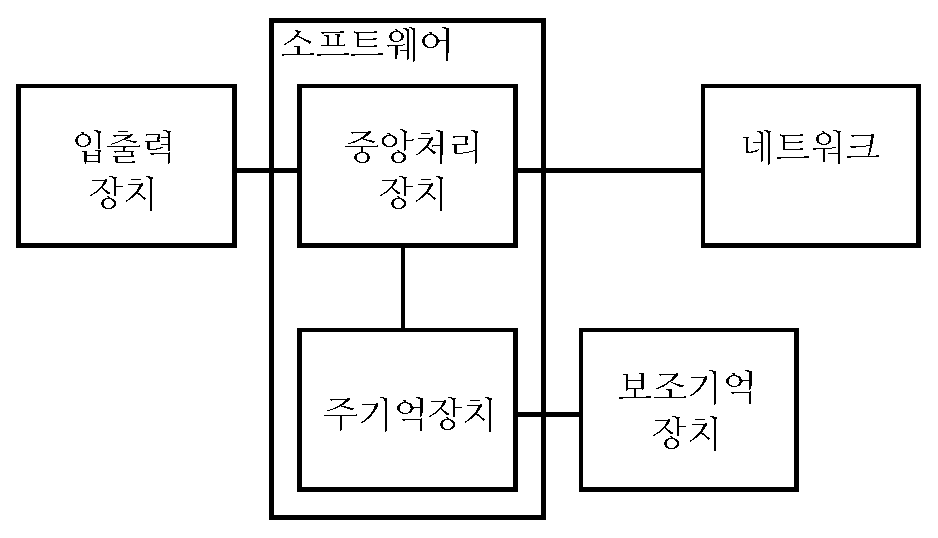
\includegraphics[height=2.50in]{figs2/arch3.eps}}
\afterfig

이번 장에서 {\bf 보조 기억장치(Secondary Memory)} 혹은 파일을 가지고 작업을 시작한다.
보조 기억장치는 전원이 꺼져도 지워지지 않는다.
혹은, USB 플래쉬 드라이브를 사용한 경우에는 프로그램으로부터 작성한 데이터는 시스템에서 제거되어 다른 시스템으로 전송될 수 있다.

우선 텍스트 편집기로 작성한 텍스트 파일을 읽고 쓰는 것에 초점을 맞출 것이다.
나중에 데이터베이스 소프트웨어를 통해서 읽고 쓰도록 설계된 바이너리 파일 데이터베이스를 가지고 어떻게 작업하는지를 살펴볼 것이다.

\section{파일 열기}
\index{파일 (file)!열기 (open)}
\index{열기 함수 (open function)}
\index{함수 (function)!열기 (open)}

하드 디스크 파일을 읽거나 쓸려고 할 때, 파일을 {\bf 열여야(open)} 한다.
파일을 열 때 각 파일 데이터가 어디에 저장되었는지를 알고 있는 운영체제와 커뮤니케이션 한다.
파일을 열 때, 운영체제에 파일이 존재하는지 확인하고 이름으로 파일을 찾도록 요청한다.     
이번 예제에서, 파이썬을 시작한 동일한 폴더에 저장된 {\tt mbox.txt} 파일을 연다.  
\url{www.py4inf.com/code/mbox.txt} 에서 파일을 다운로드할 수 있다.

\beforeverb
\begin{verbatim}
>>> fhand = open('mbox.txt')
>>> print fhand
<open file 'mbox.txt', mode 'r' at 0x1005088b0>
\end{verbatim}
\afterverb
%
\index{파일 핸들 (file handle)}

{\tt open}이 성공하면, 운영체제는 {\bf 파일 핸들(file handle)}을 반환한다.
{\bf 파일 핸들(file handle)}은 파일에 담겨진 실제 데이터는 아니고, 
대신에 데이터를 읽을 수 있도록 사용할 수 있는 ''핸들(handle)''이다.
요청한 파일이 존재하고, 파일을 읽을 수 있는 적절한 권한이 있다면 이제 핸들이 여러분에게 주어졌다.

\beforefig
\centerline{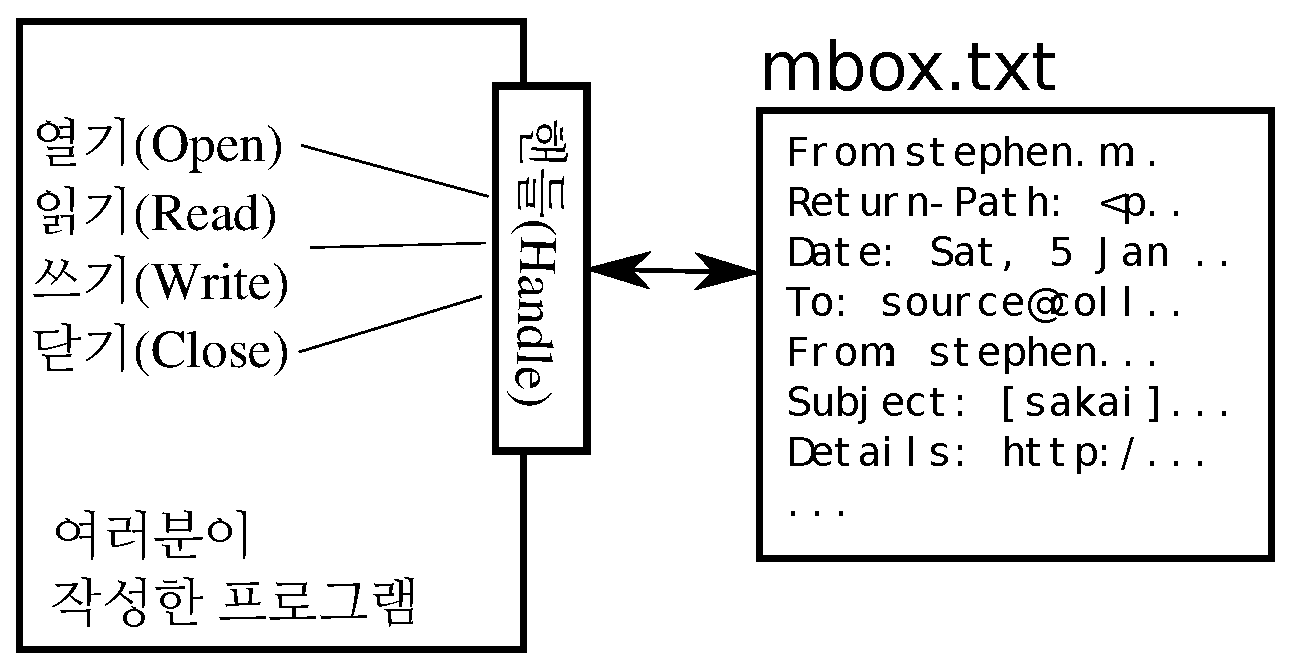
\includegraphics[height=1.75in]{figs2/handle.eps}}
\afterfig

파일이 존재하지 않는다면, {\tt open}은 역추적(traceback) 파일 열기 오류로 실패하고, 파일 콘텐츠에 접근할 핸들도 얻지 못한다.

\beforeverb
\begin{verbatim}
>>> fhand = open('stuff.txt')
Traceback (most recent call last):
  File "<stdin>", line 1, in <module>
IOError: [Errno 2] No such file or directory: 'stuff.txt'
\end{verbatim}
\afterverb
%

나중에 {\tt try}와 {\tt except}를 가지고, 존재하지 않는 파일을 열려고 하는 상황을 좀더 우아하게 처리할 것이다.

\section{텍스트 파일과 라인}

파이썬 문자열이 문자 순서(sequence)로 간주 되듯이 마찬가지로 텍스트 파일은 라인 순서(sequence)로 생각될 수 있다.
예를 들어, 다음은 오픈 소스 프로젝트 개발 팀에서 다양한 참여자들의 전자우편 활동을 기록한 텍스트 파일 샘플이다.

\beforeverb
\begin{alltt}
From stephen.marquard@uct.ac.za Sat Jan  5 09:14:16 2008
Return-Path: <postmaster@collab.sakaiproject.org>
Date: Sat, 5 Jan 2008 09:12:18 -0500
To: source@collab.sakaiproject.org
From: stephen.marquard@uct.ac.za
Subject: [sakai] svn commit: r39772 - content/branches/
Details: http://source.sakaiproject.org/viewsvn/?view=rev\&rev=39772
...
\end{alltt}
\afterverb

상호 의사소통한 전자우편 전체 파일은  \url{www.py4inf.com/code/mbox.txt} 에서 접근 가능하고, 
간략한 버젼 파일은 \url{www.py4inf.com/code/mbox-short.txt}에서 얻을 수 있다.
이들 파일은 다수 전자우편 메시지를 담고 있는 파일로 표준 포맷으로 되어 있다.
"From "으로 시작하는 라인은 메시지 본문과 구별되고, "From: "으로 시작하는 라인은 본문 메시지의 일부다.
더 자세한 정보는 \url{en.wikipedia.org/wiki/Mbox}에서 찾을 수 있다.

파일을 라인으로 쪼개기 위해서, {\bf 새줄(newline)} 문자로 불리는 "줄의 끝(end of the line)"을 표시하는 특수 문자가 있다.

\index{새줄 (newline)}

파이썬에서, 문자열 상수 역슬래쉬-n(\verb"\n")으로 {\bf 새줄(newline)} 문자를 표현한다.
두 문자처럼 보이지만, 사실은 단일 문자다. 인터프리터에 ''stuff''에 입력한 후 변수를 살펴보면, 문자열에 \verb"\n"가 있다.
하지만, {\tt print}문을 사용하여 문자열을 출력하면, 문자열이 새줄 문자에 의해서 두 줄로 쪼개지는 것을 볼 수 있다.

\beforeverb
\begin{verbatim}
>>> stuff = 'Hello\nWorld!'
>>> stuff
'Hello\nWorld!'
>>> print stuff
Hello
World!
>>> stuff = 'X\nY'
>>> print stuff
X
Y
>>> len(stuff)
3
\end{verbatim}
\afterverb
%

문자열 \verb"'X\nY'"의 길이는 \emph{3} 이다. 왜냐하면 새줄(newline) 문자도 한 문자이기 때문이다.

그래서, 파일 라인을 볼 때, 라인 끝을 표시하는 새줄(newline)로 불리는 눈에 보이지 않는 특수 문자가 각 줄의 끝에 있다고 \emph{상상}할 필요가 있다.

% \beforeverb
% \begin{alltt}
% From stephen.marquard@uct.ac.za Sat Jan  5 09:14:16 2008\verb"\n"\\
% Return-Path: <postmaster@collab.sakaiproject.org>\verb"\n"\\
% Date: Sat, 5 Jan 2008 09:12:18 -0500\verb"\n"\\
% To: source@collab.sakaiproject.org\verb"\n"\\
% From: stephen.marquard@uct.ac.za\verb"\n"\\
% Subject: [sakai] svn commit: r39772 - content/branches/\verb"\n"\\
% Details: http://source.sakaiproject.org/viewsvn/?view=rev\&rev=39772\verb"\n"\\
% ...
% \end{alltt}
% \afterverb

그래서, 새줄(newline) 문자는 파일에 있는 문자를 라인으로 분리한다.


\section{파일 읽어오기}

\index{파일 (file)!읽어 오기 (reading)}
\index{계수기 (counter)}

{\bf 파일 핸들(file handle)}이 파일 자료를 담고 있지 않지만, 
{\tt for} 루프를 사용하여 파일 각 라인을 읽고 라인수를 세는 것을 쉽게 구축할 수 있다.

\beforeverb
\begin{verbatim}
fhand = open('mbox.txt')
count = 0
for line in fhand:
    count = count + 1
print 'Line Count:', count

python open.py 
Line Count: 132045
\end{verbatim}
\afterverb
%

파일 핸들을 {\tt for} 루프 순서(sequence)로 사용할 수 있다. 
{\tt for} 루프는 단순히 파일 라인 수를 세고 전체 라인수를 출력한다.
{\tt for} 루프를 대략 일반어로 풀어 말하면, "파일 핸들로 표현되는 파일 각 라인마다, {\tt count} 변수에 1 씩 더한다"

{\tt open} 함수가 전체 파일을 바로 읽지 못하는 이유는 파일이 수 기가 바이트 파일 크기를 가질 수도 있기 때문이다.
{\tt open} 문장은 파일 크기에 관계없이 파일을 여는데 시간이 동일하게 걸린다. 
실질적으로 {\tt for} 루프가 파일로부터 자료를 읽어오는 역할을 한다.

{\tt for} 루프를 사용해서 이 같은 방식으로 파일을 읽어올 때, 새줄(newline) 문자를 사용해서 파일 자료를 라인 단위로 쪼갠다.
파이썬에서 새줄(newline) 문자까지 각 라인 단위로 읽고, 
{\tt for} 루프가 매번 반복할 때마다 {\tt line} 변수에 새줄(newline)을 마지막 문자로 포함한다.

{\tt for} 루프가 데이터를 한번에 한줄씩 읽어오기 때문에, 데이터를 저장할 주기억장치 저장공간을 소진하지 않고, 매우 큰 파일을 효과적으로 읽어서 라인을 셀 수 있다.
각 라인별로 읽고, 세고, 그리고 나서 폐기되기 때문에, 매우 적은 저장공간을 사용해서 어떤 크기의 파일도 상기 프로그램을 사용하여 라인을 셀 수 있다.

만약 주기억장치 크기에 비해서 상대적으로 작은 크기의 파일이라는 것을 안다면, 
전체 파일을 파일 핸들로 {\tt read} 메쏘드를 사용해서 하나의 문자열로 읽어올 수 있다.

\beforeverb
\begin{verbatim}
>>> fhand = open('mbox-short.txt')
>>> inp = fhand.read()
>>> print len(inp)
94626
>>> print inp[:20]
From stephen.marquar
\end{verbatim}
\afterverb
%

상기 예제에서, {\tt mbox-short.txt} 전체 파일 콘텐츠(94,626 문자)를 변수 {\tt inp}로 바로 읽었다.
문자열 슬라이싱을 사용해서 {\tt inp}에 저장된 문자열 자료 첫 20 문자를 출력한다.

파일이 이런 방식으로 읽혀질 때, 모든 라인과 새줄(newline)문자를 포함한 모든 문자는 변수 {\tt inp}에 대입된 매우 큰 문자열이다.
파일 데이터가 컴퓨터 주기억장치가 안정적으로 감당해 낼 수 있을때만, 
이런 형식의 {\tt open} 함수가 사용될 수 있다는 것을 기억하라.

만약 주기억장치가 감당해 낼 수 없는 매우 파일 크기가 크다면, {\tt for}나 {\tt while} 루프를 사용해서 파일을 쪼개서 읽는 프로그램을 작성해야 한다.

\section{파일 검색}

파일 데이터를 검색할 때, 흔한 패턴은 파일을 읽고, 대부분 라인은 건너뛰고, 특정 기준을 만족하는 라인만 처리하는 것이다.
간단한 검색 메카니즘을 구현하기 위해서 파일을 읽는 패턴과 문자열 {\bf 메쏘드}를 조합한다.

\index{필터 패턴 (filter pattern)}
\index{패턴 (pattern)!필터 (filter)}

예를 들어, 파일을 읽고, ``From:''으로 시작하는 라인만 출력하고자 한다면, 
{\bf startswith} 문자열 메쏘드를 사용해서 원하는 접두사로 시작하는 라인만을 선택한다.

\beforeverb
\begin{verbatim}
fhand = open('mbox-short.txt')
for line in fhand:
    if line.startswith('From:') :
        print line
\end{verbatim}
\afterverb
%

이 프로그램이 실행하면 다음 출력값을 얻는다.

\beforeverb
\begin{verbatim}
From: stephen.marquard@uct.ac.za

From: louis@media.berkeley.edu

From: zqian@umich.edu

From: rjlowe@iupui.edu
...
\end{verbatim}
\afterverb
%

''From:''으로만 시작하는 라인만 출력하기 때문에 출력값은 훌륭해 보인다.
하지만, 왜 여분으로 빈 라인이 보이는 걸까?
원인은 눈에 보이지 않는 {\bf 새줄(newline)} 문자 때문이다.
각 라인이 새줄(newline)로 끝나서 변수 {\bf line}에 새줄(newline)이 포함되고 
{\tt print}문이 추가로 새줄(newline)을 추가해서 결국 우리가 보기에는 두 줄 효과가 나타난다.

마지막 문자를 제외하고 모든 것을 출력하기 위해서 라인 슬라이싱(slicing)을 할수 있지만, 
좀더 간단한 접근법은 다음과 같이 문자열 오른쪽 끝에서부터 공백을 벗겨내는 {\bf rstrip} 메쏘드를 사용하는 것인다.

\beforeverb
\begin{verbatim}
fhand = open('mbox-short.txt')
for line in fhand:
    line = line.rstrip()
    if line.startswith('From:') :
        print line
\end{verbatim}
\afterverb
%

프로그램을 실행하면, 다음 출력값을 얻는다.

\beforeverb
\begin{verbatim}
From: stephen.marquard@uct.ac.za
From: louis@media.berkeley.edu
From: zqian@umich.edu
From: rjlowe@iupui.edu
From: zqian@umich.edu
From: rjlowe@iupui.edu
From: cwen@iupui.edu
...
\end{verbatim}
\afterverb
%

파일 처리 프로그램이 점점 더 복잡해짐에 따라 {\tt continue}를 사용해서 검색 루프(search loop)를 구조화할 필요가 있다.
검색 루프의 기본 아이디어는 ''흥미로운'' 라인을 집중적으로 찾고, ''흥미롭지 않은'' 라인은 효과적으로 건너뛰는 것이다.
그리고 나서 흥미로운 라인을 찾게되면, 그 라인에서 특정 연산을 수행하는 것이다.

다음과 같이 루프를 구성해서 흥미롭지 않은 라인은 건떠뛰는 패턴을 따르게 한다.

\beforeverb
\begin{verbatim}
fhand = open('mbox-short.txt')
for line in fhand:
    line = line.rstrip()
    # Skip 'uninteresting lines'
    if not line.startswith('From:') :
        continue
    # Process our 'interesting' line
    print line
\end{verbatim}
\afterverb
%

프로그램의 출력값은 동일하다. 
흥미롭지 않는 라인은 ''From:''으로 시작하지 않는 라인이라 {\tt continue}문을 사용해서 건너뛴다.
''흥미로운'' 라인 (즉, ''From:''으로 시작하는 라인)에 대해서는 연산처리를 수행한다. 

{\tt find} 문자열 메쏘드를 사용해서 검색 문자열이 라인 어디에 있는지를 찾아주는 텍스트 편집기 검색기능을 모사(simulation)할 수 있다.
{\tt find} 메쏘드는 다른 문자열 내부에 검색하는 문자열이 있는지 찾고, 문자열 위치를 반환하거나, 만약 문자열이 없다면 -1을 반환하기 때문에,
``@uct.ac.za''(남아프리카 케이프 타운 대학으로부터 왔다) 문자열을 포함하는 라인을 검색하기 위해 다음과 같이 루프를 작성한다.

\beforeverb
\begin{verbatim}
fhand = open('mbox-short.txt')
for line in fhand:
    line = line.rstrip()
    if line.find('@uct.ac.za') == -1 : 
        continue
    print line
\end{verbatim}
\afterverb
%
출력결과는 다음과 같다.

\beforeverb
\begin{verbatim}
From stephen.marquard@uct.ac.za Sat Jan  5 09:14:16 2008
X-Authentication-Warning: set sender to stephen.marquard@uct.ac.za using -f
From: stephen.marquard@uct.ac.za
Author: stephen.marquard@uct.ac.za
From david.horwitz@uct.ac.za Fri Jan  4 07:02:32 2008
X-Authentication-Warning: set sender to david.horwitz@uct.ac.za using -f
From: david.horwitz@uct.ac.za
Author: david.horwitz@uct.ac.za
...
\end{verbatim}
\afterverb
%

\section{사용자가 파일명을 선택하게 만들기}

매번 다른 파일을 처리할 때마다 파이썬 코드를 편집하고 싶지는 않다. 
매번 프로그램이 실행될 때마다, 파일명을 사용자가 입력하도록 만드는 것이 좀더 유용할 것이다. 
그래서 파이썬 코드를 바꾸지 않고, 다른 파일에 대해서도 동일한 프로그램을 사용하도록 만들자.

다음과 같이 \verb"raw_input"을 사용해서 사용자로부터 파일명을 읽어 프로그램을 실행하는 것이 단순하다.

\beforeverb
\begin{verbatim}
fname = raw_input('Enter the file name: ')
fhand = open(fname)
count = 0
for line in fhand:
    if line.startswith('Subject:') :
        count = count + 1
print 'There were', count, 'subject lines in', fname
\end{verbatim}
\afterverb
%

사용자로부터 파일명을 읽고 변수 {\tt fname}에 저장하고, 그 파일을 연다. 
이제 다른 파일에 대해서도 반복적으로 프로그램을 실행할 수 있다.

\beforeverb
\begin{verbatim}
python search6.py 
Enter the file name: mbox.txt
There were 1797 subject lines in mbox.txt

python search6.py 
Enter the file name: mbox-short.txt
There were 27 subject lines in mbox-short.txt
\end{verbatim}
\afterverb
%

다음 절을 엿보기 전에, 상기 프로그램을 살펴보고 자신에게 다음을 질문해 보자.
"여기서 어디가 잘못될 수 있는가?" 혹은 
"이 작고 멋진 프로그램에 트레이스백(traceback)을 남기고 바로 끝나게 하여,
결국 사용자 눈에는 좋지 않은 프로그램이라는 인상을 남길 수 있도록 우리의 친절한 사용자는 무엇을 할 수 있을까?

\section{{\tt try, except, open} 사용하기}

제가 여러분에게 엿보지 말라고 말씀드렸습니다. 이번이 마지막 기회입니다.
사용자가 파일명이 아닌 뭔가 다른 것을 입력하면 어떻게 될까요?

\beforeverb
\begin{verbatim}
python search6.py 
Enter the file name: missing.txt
Traceback (most recent call last):
  File "search6.py", line 2, in <module>
    fhand = open(fname)
IOError: [Errno 2] No such file or directory: 'missing.txt'

python search6.py 
Enter the file name: na na boo boo
Traceback (most recent call last):
  File "search6.py", line 2, in <module>
    fhand = open(fname)
IOError: [Errno 2] No such file or directory: 'na na boo boo'
\end{verbatim}
\afterverb
%

웃지마시구요, 사용자는 결국 여러분이 작성한 프로그램을 망가뜨리기 위해 고의든 악의를 가지든 가능한 모든 수단을 강구할 것입니다.
사실, 소프트웨어 개발팀의 중요한 부분은 {\bf 품질 보증(Quality Assurance, QA)}이라는 조직이다. 
품질보증 조직은 프로그래머가 만든 소프트웨어를 망가뜨리기 위해 가능한 말도 안 되는 것을 합니다.

\index{품질 보증 (Quality Assurance)}
\index{QA}

사용자가 소프트웨어를 제품으로 구매하거나, 주문형으로 개발하는 프로그램에 대해 월급을 지급하던지 관계없이 
품질보증 조직은 프로그램이 사용자에게 전달되기 전까지 프로그램 오류를 발견할 책임이 있다.
그래서 품질보증 조직은 프로그래머의 최고의 친구다.

\index{try 문장 (try statement)}
\index{문장 (statement)!try}
\index{open 함수 (open function)}
\index{함수 (function)!open}
\index{예외 (exception)!입출력 오류 (IOError)}
\index{입출력 오류 (IOError)}

프로그램 오류를 찾았기 때문에, {\tt try}/{\tt except} 구조를 사용해서 오류를 우아하게 고쳐봅시다.
{\tt open} 호출이 잘못될 수 있다고 가정하고, {\tt open} 호출이 실패할 때를 대비해서 다음과 같이 복구 코드를 추가한다.

\beforeverb
\begin{verbatim}
fname = raw_input('Enter the file name: ')
try:
    fhand = open(fname)
except:
    print 'File cannot be opened:', fname
    exit()

count = 0
for line in fhand:
    if line.startswith('Subject:') : 
        count = count + 1
print 'There were', count, 'subject lines in', fname
\end{verbatim}
\afterverb
%

{\tt exit}함수가 프로그램을 끝낸다. 
결코 돌아오지 않는 함수를 호출한 것이다.
이제 사용자 혹은 품질 보증 조직에서 올바르지 않거나 어처구니 없는 파일명을 입력했을 때, 
``catch''로 잡아서 우아하게 복구한다.

\beforeverb
\begin{verbatim}
python search7.py
Enter the file name: mbox.txt
There were 1797 subject lines in mbox.txt

python search7.py
Enter the file name: na na boo boo
File cannot be opened: na na boo boo
\end{verbatim}
\afterverb
%
\index{파이썬스러운 (Pythonic)}

파이썬 프로그램을 작성할 때 {\tt open} 호출을 보호하는 것은 {\tt try}, {\tt except}의 적절한 사용 예제가 된다.
''파이썬 방식(Python way)''으로 무언가를 작성할 때, ''파이썬스러운(Pythonic)''이라는 용어를 사용한다.
상기 파일을 여는 예제는 파이썬스러운 방식의 좋은 예가 된다고 말한다.

파이썬에 좀더 자신감이 생기게 되면, 다른 파이썬 프로그래머와 동일한 문제에 대해 
두 가지 동치하는 해답을 가지고 어떤 접근법이 좀더 "파이썬스러운지"에 대한 현답을 찾는데도 관여하게 된다.

"좀더 파이썬스럽게" 되는 이유는 프로그래밍이 엔지니어링적인 면과 예술적인 면을 동시에 가지고 있기 때문이다.
항상 무언가를 단지 작동하는 것에만 관심이 있지 않고, 프로그램으로 작성한 해결책이 좀더 우아하고, 다른 동료에 의해서 우아한 것으로 인정되기를 또한 원합니다.

\section{파일에 쓰기}

\index{파일 (file)!쓰기 (writing)}

파일에 쓰기 위해서는 두 번째 매개 변수로 \verb"'w'" 모드로 파일을 열어야 한다.

\beforeverb
\begin{verbatim}
>>> fout = open('output.txt', 'w')
>>> print fout
<open file 'output.txt', mode 'w' at 0xb7eb2410>
\end{verbatim}
\afterverb
%

파일이 이미 존재하는데 쓰기 모드에서 파일을 여는 것은 이전 데이터를 모두 지워버리고, 
깨끗한 파일 상태에서 다시 시작되니 주의가 필요하다. 
만약 파일이 존재하지 않는다면, 새로운 파일이 생성된다.

파일 핸들 객체의 {\tt write} 메쏘드는 데이터를 파일에 저장한다.

\beforeverb
\begin{verbatim}
>>> line1 = 'This here's the wattle,\n'
>>> fout.write(line1)
\end{verbatim}
\afterverb
%
\index{새줄 (newline)}

다시 한번, 파일 객체는 마지막 포인터가 어디에 있는지 위치를 추적해서, 
만약 {\tt write} 메쏘드를 다시 호출하게 되면, 새로운 데이터를 파일 끝에 추가한다.

라인을 끝내고 싶을 때, 명시적으로 새줄(newline) 문자를 삽입해서 파일에 쓰도록 라인 끝을 필히 관리해야 한다.

{\tt print}문은 자동적으로 새줄(newline)을 추가하지만, {\tt write} 메쏘드는 자동적으로 새줄(newline)을 추가하지는 않는다.

\beforeverb
\begin{verbatim}
>>> line2 = 'the emblem of our land.\n'
>>> fout.write(line2)
\end{verbatim}
\afterverb
%

파일 쓰기가 끝났을 때, 파일을 필히 닫아야 한다.
파일을 닫는 것은 데이터 마지막 비트까지 디스크에 물리적으로 쓰여져서, 
전원이 나가더라도 자료가 유실되지 않는 역할을 한다.

\beforeverb
\begin{verbatim}
>>> fout.close()
\end{verbatim}
\afterverb
%

파일 읽기로 연 파일을 닫을 수 있지만, 몇개 파일을 열어 놓았다면 약간 단정치 못하게 끝날 수 있습니다. 
왜냐하면 프로그램이 종료될 때 열린 모든 파일이 닫혀졌는지 파이썬이 확인하기 때문이다. 
파일에 쓰기를 할 때는, 파일을 명시적으로 닫아서 예기치 못한 일이 발생할 여지를 없애야 한다.

\index{close 메쏘드 (close method)}
\index{메쏘드 (method)!close}

\section{디버깅}

\index{디버깅 (debugging)}
\index{공백 (whitespace)}

파일을 읽고 쓸 때, 공백 때문에 종종 문제에 봉착한다.
이런 종류의 오류는 공백, 탭, 새줄(newline)이 눈에 보이지 않기 때문에 디버그하기도 쉽지 않다.

\beforeverb
\begin{verbatim}
>>> s = '1 2\t 3\n 4'
>>> print s
1 2	 3
 4
\end{verbatim}
\afterverb

\index{repr 함수 (repr function)}
\index{함수 (function)!repr}
\index{문자열 표현 (string representation)}

내장함수 {\tt repr}이 도움이 될 수 있다. 
인자로 임의 객체를 잡아 객체 문자열 표현으로 반환한다.
문자열 공백문자는 역슬래쉬 순서(sequence)로 나타냅니다.

\beforeverb
\begin{verbatim}
>>> print repr(s)
'1 2\t 3\n 4'
\end{verbatim}
\afterverb

디버깅에 도움이 될 수 있다.

여러분이 봉착하는 또 다른 문제는 다른 시스템에서는 라인 끝을 표기하기 위해서 다른 문자를 사용한다는 점이다.
어떤 시스템은 \verb"\n" 으로 새줄(newline)을 표기하고, 다른 시스템은 \verb"\r"으로 반환 문자(return character)를 사용한다.
둘다 모두 사용하는 시스템도 있다. 
파일을 다른 시스템으로 이식한다면, 이러한 불일치가 문제를 야기한다.

\index{라인 끝 문자 (end of line character)}

대부분의 시스템에는 A 포맷에서 B 포멧으로 변환하는 응용프로그램이 있다.
\url{wikipedia.org/wiki/Newline} 에서 응용프로그램을 찾을 수 있고, 좀더 많은 것을 읽을 수 있다.
물론, 여러분이 직접 프로그램을 작성할 수도 있다.

% TBD - Doesn't Python take care of this for us????

\section{용어정의}

\begin{description}

\item[잡기(catch):] {\tt try}와 {\tt except} 문을 사용해서 프로그램이 끝나는 예외 상황을 방지하는 것.
\index{잡기 (catch)}

\item[새줄(newline):] 라인의 끝을 표기 위한 파일이나 문자열에 사용되는 특수 문자.
\index{새줄 (newline)}

\item[파이썬스러운(Pythonic):] 파이썬에서 우아하게 작동하는 기술. ''try와 catch를 사용하는 것은 파일이 없는 경우를 복구하는 파이썬스러운 방식이다.''
\index{파이썬스러운 (Pythonic)}

\item[품질 보증(Quality Assurance, QA):] 소프트웨어 제품의 전반적인 품질을 보중하는데 집중하는 사람이나 조직.
품질 보증은 소프트웨어 제품을 시험하고, 제품이 시장에 출시되기 전에 문제를 확인하는데 관여한다.
\index{품질 보증 (Quality Assurance)}
\index{QA}

\item[텍스트 파일(text file):] 하드디스크 같은 영구 저장소에 저장된 일련의 문자 집합.
\index{텍스트 파일 (text file)}

\end{description}

\section{연습문제}

\begin{ex}
파일을 읽고 한줄씩 파일의 내용을 모두 대문자로 출력하는 프로그램을 작성하세요.
프로그램을 싱행하면 다음과 같이 보일 것입니다.

\beforeverb
\begin{verbatim}
python shout.py
Enter a file name: mbox-short.txt
FROM STEPHEN.MARQUARD@UCT.AC.ZA SAT JAN  5 09:14:16 2008
RETURN-PATH: <POSTMASTER@COLLAB.SAKAIPROJECT.ORG>
RECEIVED: FROM MURDER (MAIL.UMICH.EDU [141.211.14.90])
	 BY FRANKENSTEIN.MAIL.UMICH.EDU (CYRUS V2.3.8) WITH LMTPA;
	 SAT, 05 JAN 2008 09:14:16 -0500
\end{verbatim}
\afterverb
%
\url{www.py4inf.com/code/mbox-short.txt}에서 파일을 다운로드 받으세요.
\end{ex}

\begin{ex}

파일명을 입력받아, 파일을 읽고, 다음 형식의 라인을 찾는 프로그램을 작성하세요.

\beforeverb
\begin{alltt}
X-DSPAM-Confidence: {\bf 0.8475}
\end{alltt}
\afterverb

``X-DSPAM-Confidence:''로 시작하는 라인을 만나게 되면, 부동 소수점 숫자를 뽑아내기 위해 해당 라인을 별도로 보관하세요.
라인 수를 세고, 라인으로부터 스팸 신뢰값의 총계를 계산하세요. 
파일의 끝에 도달할 했을 때, 평균 스팸 신뢰도를 출력하세요.

\beforeverb
\begin{verbatim}
Enter the file name: mbox.txt
Average spam confidence: 0.894128046745

Enter the file name: mbox-short.txt
Average spam confidence: 0.750718518519
\end{verbatim}
\afterverb
%
{\tt mbox.txt}와 {\tt mbox-short.txt} 파일에 작성한 프로그램을 시험하세요.
\end{ex}

\begin{ex}

때때로, 프로그래머가 지루해지거나, 약간 재미를 목적으로, 프로그램에 무해한 {\bf 부활절 달걀}(Easter Egg, \url{en.wikipedia.org/wiki/Easter_egg_(media)})을 넣습니다.
사용자가 파일명을 입력하는 프로그램을 변형시켜, 'na na boo boo'로 파일명을 정확하게 입력했을 때, 재미있는 메시지를 출력하는 프로그램을 작성하세요.
파일이 존재하거나, 존재하지 않는 다른 모든 파일에 대해서도 정상적으로 작동해야 합니다. 
여기 프로그램을 실행한 견본이 있습니다.

\beforeverb
\begin{verbatim}
python egg.py 
Enter the file name: mbox.txt
There were 1797 subject lines in mbox.txt

python egg.py 
Enter the file name: missing.tyxt
File cannot be opened: missing.tyxt

python egg.py 
Enter the file name: na na boo boo
NA NA BOO BOO TO YOU - You have been punk'd!
\end{verbatim}
\afterverb
%

프로그램에 부활절 달걀을 넣도록 격려하지는 않습니다. 단지 연습입니다.

\end{ex}


%% LaTeX source for ``Python for Informatics: Exploring Information''
% Copyright (c)  2010-  Charles R. Severance, All Rights Reserved

\chapter{리스트}

\index{list}
\index{type!list}


\section{리스트는 열이다.}

문자열처럼, {\bf 리스트(list)}는 일련의 값이다. 문자열에서, 값은 문자지만, 리스트에서는 임의의 형(type)이 될 수 있다.
리스트의 값은 {\bf 요소(elements)}나 때때로 {\bf 항목(items)}으로 불린다.

\index{element}
\index{sequence}
\index{item}

신규 리스틀 생성하는 방법은 여러가지다. 가장 간단한 방법은 꺾쇠 괄호(\verb"[" 와 \verb"]")로 요소를 감싸는 것이다.

\beforeverb
\begin{verbatim}
[10, 20, 30, 40]
['crunchy frog', 'ram bladder', 'lark vomit']
\end{verbatim}
\afterverb
%
첫번째 예제는 네 개의 정수 리스트다. 드번째 예제는 3개의 문자열 리스트다.
문자열의 요소는 같은 형(type)일 필요는 없다. 다음의 리스트는 문자열, 부동 소수점 숫자, 정수, (아!) 또 다른 리스트를 담고 있다.

\beforeverb
\begin{verbatim}
['spam', 2.0, 5, [10, 20]]
\end{verbatim}
\afterverb
%

또 다른 리스트 내부에 리스트는 {\bf 중첩(nested)}되어 있다.

\index{nested list}
\index{list!nested}

어떤 요소도 담고 있지 않는 리스트는 빈 리스트(empty list)라고 부르고, 빈 꺾쇠 괄호(''[]'')로 생성할 수 있다.

\index{empty list}
\index{list!empty}

예상했듯이, 리스트 값을 변수에 할당할 수 있다.

\beforeverb
\begin{verbatim}
>>> cheeses = ['Cheddar', 'Edam', 'Gouda']
>>> numbers = [17, 123]
>>> empty = []
>>> print cheeses, numbers, empty
['Cheddar', 'Edam', 'Gouda'] [17, 123] []
\end{verbatim}
\afterverb
%

\index{assignment}

\section{리스트는 변경가능하다.}

\index{list!element}
\index{access}
\index{index}
\index{bracket operator}
\index{operator!bracket}

리스트의 요소에 접근하는 구문은 문자열의 문자에 접근하는 것과 동일한 꺾쇠 괄호 연산자다.
꺽쐬 괄호 내부의 표현식은 인덱스를 명세한다. 인덱스는 0 에서부터 시작한다.

\beforeverb
\begin{verbatim}
>>> print cheeses[0]
Cheddar
\end{verbatim}
\afterverb
%

문자열과 달리, 리스트의 항목의 순서를 바꾸거나, 리스트에 새로운 항목을 재할당할 수 있기 때문에 리스트는 변경가능하다.
꺾쇠 괄호 연산자가 할당문의 왼쪽편에 나타날 때, 새로 할당될 리스트의 요소를 나타낸다.

\index{mutability}

\beforeverb
\begin{verbatim}
>>> numbers = [17, 123]
>>> numbers[1] = 5
>>> print numbers
[17, 5]
\end{verbatim}
\afterverb
%

리스트 {\tt numbers}의 1번째 요소는 123 값을 가지고 있으나, 이제는 5 값을 가진다.

\index{index!starting at zero}
\index{zero, index starting at}

리스트를 인텍스와 요소의 관계로 생각할 수 있다. 이 관계를 {\bf 매핑(mapping)}이라고 부른다. 각각의 인덱스는 요소중의 하나에 대응(''maps to'')된다.

\index{item assignment}
\index{assignment!item}

리스트 인덱스는 문자열 인덱스와 같은 방식으로 동작한다.

\begin{itemize}

\item 임의의 정수 표현식은 인덱스로 사용될 수 있다.

\item 존재하지 않는 요소를 읽거나 쓰려고 하면, {\tt IndexError}가 발생한다.

\index{exception!IndexError}
\index{IndexError}

\item 인덱스가 음의 값이면, 리스트의 끝에서부터 역으로 센다.

\end{itemize}

\index{list!index}

\index{list!membership}
\index{membership!list}
\index{in operator}
\index{operator!in}


{\tt in} 연산자도 또한 리스트에서 동작한다.

\beforeverb
\begin{verbatim}
>>> cheeses = ['Cheddar', 'Edam', 'Gouda']
>>> 'Edam' in cheeses
True
>>> 'Brie' in cheeses
False
\end{verbatim}
\afterverb


\section{리스트 운행법}
\index{list!traversal}
\index{traversal!list}
\index{for loop}
\index{loop!for}
\index{statement!for}

리스트의 요소를 운행하는 가장 흔한 방법은 {\tt for}문을 사용하는 것이다.
구문은 문자열에서 사용한 것과 동일하다.

\beforeverb
\begin{verbatim}
for cheese in cheeses:
    print cheese
\end{verbatim}
\afterverb
%

리스트의 요소를 읽기만 한다면 이것만으로 잘 동작한다. 하지만, 리스트의 요소를 쓰거나, 갱신하는 경우,
인텍스가 필요하다. 리스트의 요소를 쓰거나 갱신하는 흔한 방법은 {\tt range}와 {\tt len} 함수를 조합하는 것이다.

\index{looping!with indices}
\index{index!looping with}

\beforeverb
\begin{verbatim}
for i in range(len(numbers)):
    numbers[i] = numbers[i] * 2
\end{verbatim}
\afterverb
%

상기 루프는 리스트를 운행하고 각 요소를 갱신한다. {\tt len}함수는 리스트의 요소의 갯수를 반환한다.
{\tt range} 함수는 0 에서 $n-1$ 까지 리스트 인텍스를 반환한다. 여기서, $n$은 리스트의 길이다.
매번 루프가 반복될 때마다, {\tt i}는 다음 요소의 인덱스를 얻는다. 몸통 부문의 할당문은 {\tt i}를 사용해서 요소의 옛값을 일고 새값을 할당한다.

\index{item update}
\index{update!item}

빈 리스트의 {\tt for}문은 결코 몸통부분을 실행하지 않는다.

\beforeverb
\begin{verbatim}
for x in empty:
    print 'This never happens.'
\end{verbatim}
\afterverb
%

리스트가 또 다른 리스트를 담을 수 있지만, 중첩된 리스트는 여전히 하나의 요소로 센다. 다음 리스트의 길이는 4이다.

\index{nested list}
\index{list!nested}

\beforeverb
\begin{verbatim}
['spam', 1, ['Brie', 'Roquefort', 'Pol le Veq'], [1, 2, 3]]
\end{verbatim}
\afterverb

\section{리스트 연산자}
\index{list!operation}

{\tt +} 연산자는 리스트를 결합한다.

\index{concatenation!list}
\index{list!concatenation}

\beforeverb
\begin{verbatim}
>>> a = [1, 2, 3]
>>> b = [4, 5, 6]
>>> c = a + b
>>> print c
[1, 2, 3, 4, 5, 6]
\end{verbatim}
\afterverb
%
유사하게 {\tt *} 연산자는 주어진 횟수 만큼 리스트를 반복한다.

\index{repetition!list}
\index{list!repetition}

\beforeverb
\begin{verbatim}
>>> [0] * 4
[0, 0, 0, 0]
>>> [1, 2, 3] * 3
[1, 2, 3, 1, 2, 3, 1, 2, 3]
\end{verbatim}
\afterverb
%

첫 예제는 {\tt [0]}을 4회 반복한다. 두 번째 예제는 {\tt [1, 2, 3]} 리스트를 3회 반복한다.

\section{리스트 쪼개기(List slices)}

\index{slice operator}
\index{operator!slice}
\index{index!slice}
\index{list!slice}
\index{slice!list}

쪼개는 연산자는 리스트에도 동작한다.

\beforeverb
\begin{verbatim}
>>> t = ['a', 'b', 'c', 'd', 'e', 'f']
>>> t[1:3]
['b', 'c']
>>> t[:4]
['a', 'b', 'c', 'd']
>>> t[3:]
['d', 'e', 'f']
\end{verbatim}
\afterverb
%
첫 번째 인덱스를 생략하면, 쪼개기는 처음부터 시작한다. 두 번째 인덱스를 생략하면, 쪼개기는 끝까지 간다.
그래서 양쪽의 인덱스를 생략하면, 쪼개기는 전체 리스트를 복사한다.

\index{list!copy}
\index{slice!copy}
\index{copy!slice}

\beforeverb
\begin{verbatim}
>>> t[:]
['a', 'b', 'c', 'd', 'e', 'f']
\end{verbatim}
\afterverb
%

리스트는 변경이 가능하기 때문에 리스트를 접고, 돌리고, 훼손하는 연ㅅ나을 수행하기 전에 사본을 만드는 것이 유용하다.

\index{mutability}

할당문의 왼편의 쪼개기 연산자는 복수의 요소를 갱신할 수 있다.

\index{slice!update}
\index{update!slice}

\beforeverb
\begin{verbatim}
>>> t = ['a', 'b', 'c', 'd', 'e', 'f']
>>> t[1:3] = ['x', 'y']
>>> print t
['a', 'x', 'y', 'd', 'e', 'f']
\end{verbatim}
\afterverb
%

\section{리스트 메쏘드}

\index{list!method}
\index{method, list}

파이썬은 리스트에 연산하는 메쏘드를 제공한다. 예를 들어, {\tt append} 메쏘드는 리스트 끝에 신규 요소를 추가한다.

\index{append method}
\index{method!append}

\beforeverb
\begin{verbatim}
>>> t = ['a', 'b', 'c']
>>> t.append('d')
>>> print t
['a', 'b', 'c', 'd']
\end{verbatim}
\afterverb
%
{\tt extend} 메쏘드는 인수로 리스트를 받아 모든 요소를 리스트에 추가한다.

\index{extend method}
\index{method!extend}

\beforeverb
\begin{verbatim}
>>> t1 = ['a', 'b', 'c']
>>> t2 = ['d', 'e']
>>> t1.extend(t2)
>>> print t1
['a', 'b', 'c', 'd', 'e']
\end{verbatim}
\afterverb
%

상기 예제는 {\tt t2} 리스트를 변경없이 놓아둔다.

{\tt sort} 메쏘드는 낮음에서 높음으로 리스트의 요소를 정렬한다.

\index{sort method}
\index{method!sort}

\beforeverb
\begin{verbatim}
>>> t = ['d', 'c', 'e', 'b', 'a']
>>> t.sort()
>>> print t
['a', 'b', 'c', 'd', 'e']
\end{verbatim}
\afterverb
%

대부분의 리스트 메쏘드는 보이드(void)여서, 리스트를 변경하고 {\tt None}을 반환한다.
우연히 {\tt t = t.sort()} 이렇게 작성한다면, 결과에 실망할 것이다.

\index{void method}
\index{method!void}
\index{None special value}
\index{special value!None}

\section{요소 삭제}

\index{element deletion}
\index{deletion, element of list}

리스트에서 요소를 삭제하는 몇 가지 방법이 있다. 리스트 요소 인덱스를 알고 있다면, {\tt pop} 메쏘드를 사용한다.

\index{pop method}
\index{method!pop}

\beforeverb
\begin{verbatim}
>>> t = ['a', 'b', 'c']
>>> x = t.pop(1)
>>> print t
['a', 'c']
>>> print x
b
\end{verbatim}
\afterverb
%

{\tt pop} 메쏘드는 리스트를 변경하여  제거된 요소를 반환한다.
인덱스를 주지 않으면, 마지막 요소를 지우고 반환한다.

요소에서 제거된 값이 필요없다면, {\tt del} 연산자를 사용할 수 있다.

\index{del operator}
\index{operator!del}

\beforeverb
\begin{verbatim}
>>> t = ['a', 'b', 'c']
>>> del t[1]
>>> print t
['a', 'c']
\end{verbatim}
\afterverb
%

인덱스가 아닌 제거할 요소를 알고 있다면, {\tt remove} 메쏘드를 사용할 수 있다.

\index{remove method}
\index{method!remove}

\beforeverb
\begin{verbatim}
>>> t = ['a', 'b', 'c']
>>> t.remove('b')
>>> print t
['a', 'c']
\end{verbatim}
\afterverb
%

{\tt remove} 메쏘드의 반환값은 {\tt None}이다.

\index{None special value}
\index{special value!None}

하나 이상의 요소를 제거하기 위해서, 쪼개기 인덱스(slice index)와 {\tt del}을 사용한다.

\beforeverb
\begin{verbatim}
>>> t = ['a', 'b', 'c', 'd', 'e', 'f']
>>> del t[1:5]
>>> print t
['a', 'f']
\end{verbatim}
\afterverb
%

마찬가지로, 쪼개기는 두 번째 인덱스를 포함하지 않는 두 번째 인덱스까지의 모든 요소를 선택한다.

\section{리스트와 함수}

루프를 작성하지 않고 리스트를 빠를게 살펴볼 수 있도록 리스트에 적용할 수 있는 많은 내장함수가 있다.

\beforeverb
\begin{verbatim}
>>> nums = [3, 41, 12, 9, 74, 15]
>>> print len(nums)
6
>>> print max(nums)
74
>>> print min(nums)
3
>>> print sum(nums)
154
>>> print sum(nums)/len(nums)
25
\end{verbatim}
\afterverb
%

리스트 요소가 숫자일 때, {\tt sum()} 함수는 동작한다. {\tt max()}, {\tt len()}, 등등의 함수는 문자열 리스트나,
 비교가능한 다른 형(type)의 리스트에 사용할 수 있다.

리스트를 사용해서, 사용자가 입력한 숫자 목록의 평균을 계산하는 앞서 작성한 프로그램을 다시 작성할 수 있다.

우선 리스트 없이 평균을 계산하는 프로그램:

\beforeverb
\begin{verbatim}
total = 0
count = 0
while ( True ) :
    inp = raw_input('Enter a number: ')
    if inp == 'done' : break
    value = float(inp)
    total = total + value
    count = count + 1

average = total / count
print 'Average:', average
\end{verbatim}
\afterverb
%
이 프로그램에서, {\tt count} 와 {\tt sum} 변수를 사용해서 반복적으로 사용자가 숫자를 입력하면 값을 저장하고, 
지금까지 사용자가 입력한 누적 합계를 계산하는 것이다.

단순하게, 사용자가 입력한 각 숫자를 기억하고 내장함수를 사용해서 프로그램 마지막에 합계와 갯수를 계산한다.

\beforeverb
\begin{verbatim}
numlist = list()
while ( True ) :
    inp = raw_input('Enter a number: ')
    if inp == 'done' : break
    value = float(inp)
    numlist.append(value)

average = sum(numlist) / len(numlist)
print 'Average:', average
\end{verbatim}
\afterverb
%

루프가 시작되기 전에 빈 리스트를 생성하고, 매번 숫자를 입력할 때, 숫자를 리스트에 추가한다.
프로그램 마지막에 간단하게 리스트의 합계를 계산하고, 평균을 출력하기 위해서 입력한 숫자 개수로 나누었다.

\section{리스트와 문자열}

\index{list}
\index{string}
\index{sequence}

문자열은 일련의 문자이고, 리스트는 일련의 값이다. 하지만 리스트의 문자는 문자열과 같지는 않다. 문자열에서 리스트의 문자로 변환하기 위해서, 
{\tt list}를 사용한다.

\index{list!function}
\index{function!list}

\beforeverb
\begin{verbatim}
>>> s = 'spam'
>>> t = list(s)
>>> print t
['s', 'p', 'a', 'm']
\end{verbatim}
\afterverb
%

{\tt list}는 내장함수의 이름이기 때문에, 변수명으로 사용하는 것을 피해야 한다.
{\tt l}의 사용을 {\tt 1} 처럼 보이기 때문에 피한다. 그래서, {\tt t}를 사용하였다.

{\tt list} 함수는 문자열을 각각의 문자로 쪼갠다. 문자열을 단어로 쪼개려면, {\tt split} 메쏘드를 사용할 수 있다.

\index{split method}
\index{method!split}

\beforeverb
\begin{verbatim}
>>> s = 'pining for the fjords'
>>> t = s.split()
>>> print t
['pining', 'for', 'the', 'fjords']
>>> print t[2]
the
\end{verbatim}
\afterverb
%
{\tt split} 메쏘드를 사용해서 문자열을 리스트의 토큰으로 쪼개기만 하면, 인덱스 연산자('[]')를 사용하여 리스트의 특정한 단어를 볼 수 있다.

{\bf 구분자(delimiter)}가 단어의 경계로 어느 문자를 사용할지를 지정하는데, {\tt split} 메쏘드를 호출할 때 두 번째 선택 인수로 사용할 수 있다.
다음 예제는 구분자로 하이픈('-')을 사용한다.

\index{optional argument}
\index{argument!optional}
\index{delimiter}

\beforeverb
\begin{verbatim}
>>> s = 'spam-spam-spam'
>>> delimiter = '-'
>>> s.split(delimiter)
['spam', 'spam', 'spam']
\end{verbatim}
\afterverb
%

{\tt join} 메쏘드는 {\tt split} 메쏘드의 역이다. 문자열 리스트를 받아 리스트 요소를 결합한다.
{\tt join}은 문자열 메쏘드여서, 구분자를 호출하여 매개 변수로 넘길 수 있다.

\index{join method}
\index{method!join}
\index{concatenation}

\beforeverb
\begin{verbatim}
>>> t = ['pining', 'for', 'the', 'fjords']
>>> delimiter = ' '
>>> delimiter.join(t)
'pining for the fjords'
\end{verbatim}
\afterverb
%

상기의 경우, 구분자가 공백 문자여서 {\tt join} 메쏘드는 단어 사이에 공백을 넣는다.
공백없이 문자열을 결합하기 위해서, 구분자로 빈 문자열 \verb"''"을 사용한다.

\index{empty string}
\index{string!empty}


\section{라인을 파싱하기}

파일을 읽을 때 통상, 단지 전체 라인을 출력하는 것 말고 뭔가 다른 것을 하고자 한다.
종종 ''흥미로운 라인을'' 찾아서 라인을 파싱하여 흥미로운 \emph{ 부분(parse)}을 찾고자 한다.
``From ''으로 시작하는 라인에서 요일을 찾고자 하면 어떨까?

\beforeverb
\begin{alltt}
From stephen.marquard@uct.ac.za {\bf Sat} Jan  5 09:14:16 2008
\end{alltt}
\afterverb

{\tt split} 메쏘드는 이런 종류의 문제에 직면했을 때, 매우 효과적이다.
''From ''으로 시작하는 라인을 찾고 {\tt split} 메쏘드로 파싱하고 라인의 흥미로운 부분을 출력하는 작은 프로그램을 작성할 수 있다.

\beforeverb
\begin{verbatim}
fhand = open('mbox-short.txt')
for line in fhand:
    line = line.rstrip()
    if not line.startswith('From ') : continue
    words = line.split()
    print words[2]
\end{verbatim}
\afterverb
%

{\tt if} 문의 축약 형태로 {\tt continue }문을 {\tt if}문과 동일한 라인에 놓았다.
{\tt if} 문의 축약 형태는 {\tt continue }문을 다음 라인에 들여쓰기를 한 것과 동일하다.

프로그램은 다음을 출력한다.

\beforeverb
\begin{verbatim}
Sat
Fri
Fri
Fri
    ...
\end{verbatim}
\afterverb
%

나중에, 작업할 라인을 선택하고, 탐색하는 정확한 비트(bit) 수준의 정보를 찾아 내기 위해서 어떻게 해당 라인에서 뽑아내는 정교한 기술에 대해서 배울 것이다.

\section{개체와 값(value)}

\index{object}
\index{value}

아래 할당문을 실행한다.

\beforeverb
\begin{verbatim}
a = 'banana'
b = 'banana'
\end{verbatim}
\afterverb
%

{\tt a} 와 {\tt b} 모두 문자열을 참조하지만, 두 변수가 \emph{동일한} 문자열을 참조하는지 알 수 없다.

두 가지 가능한 상태가 있다.

\index{aliasing}

\beforefig
\centerline{\includegraphics{figs2/list1.eps}}
\afterfig

한 가지 경우는 {\tt a} 와 {\tt b}가 같은 값을 가지는 다른 두 개체를 참조하는 것이다. 두번째 경우는 같은 개체를 참조하는 것이다.

\index{is operator}
\index{operator!is}

두 변수가 동일한 개체를 참조하는지를 확인하기 위해서, {\tt is} 연산자가 사용된다.

\beforeverb
\begin{verbatim}
>>> a = 'banana'
>>> b = 'banana'
>>> a is b
True
\end{verbatim}
\afterverb
%

이 경우, 파이썬은 하나의 문자열 개체를 생성하고 {\tt a} 와 {\tt b} 모두 동일한 개체를 참조한다.

하지만, 두개의 리스트를 생성할 때, 두 개의 개체를 얻게된다.

\beforeverb
\begin{verbatim}
>>> a = [1, 2, 3]
>>> b = [1, 2, 3]
>>> a is b
False
\end{verbatim}
\afterverb
%

상기의 경우, 두개의 리스트는 동등하다고 말할 수 있다. 왜냐하면 동일한 요소를 가지고 있기 때문이다.
하지만, 같은 개체는 아니기 때문에 동일하지는 않다. 두개의 개체가 동일하다면, 두 개체는 또한 등등하다.
하지만, 동등하다고 해서 반듯이 동일하지는 않다.

\index{equivalence}
\index{identity}

지금까지 ''개체''와 ''값(value)''를 구분없이 사용했지만, 개체가 값을 가진다라고 말하는 것이는 좀더 정확하다.
{\tt a = [1,2,3]} 을 실행하면, {\tt a} 는 리스트 개체로 특별한 일련의 요소값을 가진다. 만약 또 다른 리스트가 동일한 요소를 가진다면,
그 리스트느 같은 값을 가진다고 말한다.

\index{object}
\index{value}


\section{에일리어싱(Aliasing)}

\index{aliasing}
\index{reference!aliasing}

{\tt a}가 개체를 참조하고, {\tt b = a} 할당하다면, 두 변수는 동일한 개체를 참조한다.

\beforeverb
\begin{verbatim}
>>> a = [1, 2, 3]
>>> b = a
>>> b is a
True
\end{verbatim}
\afterverb
%

개체 변수의 연관을 {\bf 참조(reference)}라고 한다. 상기의 경우 동일한 개체를 두 개의 참조가 있다.

\index{reference}

하나 이상의 참조를 가진 개체는 한개 이상의 이름을 가져서 개체가 {\bf 에일리어스(aliased)} 되었다고 한다.

\index{mutability}

만약 에일리어스된 개체가 변경 가능하면, 변화의 여파는 다른 개체에도 파급된다.

\beforeverb
\begin{verbatim}
>>> b[0] = 17
>>> print a
[17, 2, 3]
\end{verbatim}
\afterverb
%

이런 행동이 유용하기도 하지만, 오류를 발생하기도 쉽다. 일반적으로, 변경가능한 개체(mutable object)로 작업할 때 에일리어싱을 피하는 것이 안전하다.

\index{immutability}

문자열 같은 변경 불가능한 개체에 에일리어싱은 그다지 문제가 되지 않는다. 

\beforeverb
\begin{verbatim}
a = 'banana'
b = 'banana'
\end{verbatim}
\afterverb
%
상기 예제에서, {\tt a} 와 {\tt b}가 동일한 문자열을 참조하든 참조하지 않든 거의 차이가 없다.

\section{리스트 인수}

\index{list!as argument}
\index{argument}
\index{argument!list}
\index{reference}
\index{parameter}

리스트를 함수에 인수로 전달할 때, 함수는 리스트의 참조를 얻는다. 만약 함수가 리스트 매개 변수를 변경한다면, 호출자는 변화를 보게된다.
예를 들어, \verb"delete_head"는 리스트로부터 첫 요소를 제거한다.

\beforeverb
\begin{verbatim}
def delete_head(t):
    del t[0]
\end{verbatim}
\afterverb
%

여기 어떻게 \verb"delete_head" 함수가 사용된 예제가 있다.

\beforeverb
\begin{verbatim}
>>> letters = ['a', 'b', 'c']
>>> delete_head(letters)
>>> print letters
['b', 'c']
\end{verbatim}
\afterverb
%

매개 변수 {\tt t}와 변수 {\tt letters}는 동일한 개체에 대한 에일리어스(aliases)다.

리스트를 변경하는 연산자와 신규 리스트를 생성하는 연산자를 구별하는 것은 중요하다.
예를 들어, {\tt append} 메쏘드는 리스트를 변경하지만, {\tt +} 연산자는 신규 리스트를 생성한다.

\index{append method}
\index{method!append}
\index{list!concatenation}
\index{concatenation!list}

\beforeverb
\begin{verbatim}
>>> t1 = [1, 2]
>>> t2 = t1.append(3)
>>> print t1
[1, 2, 3]
>>> print t2
None

>>> t3 = t1 + [3]
>>> print t3
[1, 2, 3]
>>> t2 is t3
False
\end{verbatim}
\afterverb

리스트를 변경하는 함수를 작성할 때, 이 차이는 매우 중요하다.
예를 들어, 다음의 함수는 리스트의 처음(head)을 삭제하지 않는다.

\beforeverb
\begin{verbatim}
def bad_delete_head(t):
    t = t[1:]              # 틀림(WRONG)!
\end{verbatim}
\afterverb

슬라이스 연산자는 새로운 리스트를 생성하지만, 인수로 전달된 리스트에는 어떠한 영향도 주지 못한다.

\index{slice operator}
\index{operator!slice}

대안은 신규 리스트를 생성하고 반환하는 함수를 작성하는 것이다. 예를 들어, {\tt tail}은 리스트의 첫 요소를 제외하고 모든 요소를 반환한다.

\beforeverb
\begin{verbatim}
def tail(t):
    return t[1:]
\end{verbatim}
\afterverb
%

상기 함수는 원 리시트를 변경하지는 않는다. 여기 어떻게 사용되었는지 예시가 있다.

\beforeverb
\begin{verbatim}
>>> letters = ['a', 'b', 'c']
>>> rest = tail(letters)
>>> print rest
['b', 'c']
\end{verbatim}
\afterverb


\begin{ex}

리스트를 인수로 받아 리스트를 변경하여, 첫번째 요소와 마지막 요소를 제거하고 {\tt None}을 반환하는 {\tt chop} 함수를 작성하게요.

그리고 나서, 리스트를 인수로 받아 처음과 마지막 요소를 제외한 나머지 요소를 새로운 리스트로 반환하는 {\tt middle} 함수를 작성하세요.

\end{ex}


\section{디버깅}
\index{debugging}

부주의한 리스트의 사용이나 다른 변경가능한 재체를 사용하는 경우 오랜 시간의 디버깅으로 이끌 수 있다. 몇몇 일반적인 함정과 회피하는 방법을 소개한다.

\begin{enumerate}

\item 대부분의 리스트 메쏘드는 인수를 변경하고, {\tt None}을 반환한다. 이는 새로운 문자열을 반환하고 원 문자열은 그대로 두는 문자열과 정반대다.

다음과 같이 문자열 코드를 쓰는데 익숙해져 있다면,

\beforeverb
\begin{verbatim}
word = word.strip()
\end{verbatim}
\afterverb

다음과 같이 리스트 코드를 작성하고 싶은 유혹이 있을 것이다.

\beforeverb
\begin{verbatim}
t = t.sort()           # 틀림(WRONG)!
\end{verbatim}
\afterverb

\index{sort method}
\index{method!sort}

{\tt sort} 메쏘드는 {\tt None}을 반환하기 때문에, 리스트 {\tt t}에 수행한 다음 연산은 수행되지 않는다.

리스트를 사용한 메쏘드와 연산자를 사용하기 전에, 문서를 주의깊게 읽고, 인터랙티브 모드에서 시험하는 것을 권한다.
리스트가 문자열과 같은 다른 열과 공유하는 메쏘드와 연산자는 \url{docs.python.org/lib/typesseq.html} 에 문서화되어 있다.
변경가능한 열에만 적용되는 메쏘드와 연산자는 \url{docs.python.org/lib/typesseq-mutable.html}에 문서화되어 있다.



\item 관용구를 선택하고 고수하라.
\index{idiom}

리스트와 관련된 문제의 일부는 리스트를 가지고 할 수 있는 것이 너무 많다는 것이다.
예를 들어, 리스트에서 요소를 제거하기 위해서, {\tt pop}, {\tt remove}, {\tt del}, 혹은 쪼개기 할당(slice assignment)도 사용할 수 있다.
요소를 추가하기 위해서 {\tt append} 메쏘드나 {\tt +} 연산자를 사용할 수 있다. 하지만 다음이 맞다는 것을 잊지 마세요.

\beforeverb
\begin{verbatim}
t.append(x)
t = t + [x]
\end{verbatim}
\afterverb

하지만, 다음은 잘못됐다.

And these are wrong:

\beforeverb
\begin{verbatim}
t.append([x])          # 틀림(WRONG)!
t = t.append(x)        # 틀림(WRONG)!
t + [x]                # 틀림(WRONG)!
t = t + x              # 틀림(WRONG)!
\end{verbatim}
\afterverb

인터랙티브 모드에서 각각을 연습해 보해서 제대로 이해하고 있는지 확인해 보세요.
마지막 두개만이 실행 오류를 하고, 다른 세가지는 모두 작동하지만, 잘못된 것을 수행함을 주목하세요.

\item 에일리어싱을 피하기 위해서 사본 만들기.

\index{aliasing!copying to avoid}
\index{copy!to avoid aliasing}

인수를 변경하는 {\tt sort}같은 메쏘드를 사용하지만, 원 리스트도 보관하길 원한다면, 사본을 만들 수 있다.

\beforeverb
\begin{verbatim}
orig = t[:]
t.sort()
\end{verbatim}
\afterverb

상기 예제에 원 리스트는 그대로 둔 상태로 새로 정렬된 리스트를 반환하는 내장함수 {\tt sorted}를 사용할 수 있다.
하지만 이 경우에는, 변수명으로 {\tt sorted}를 사용하는 것을 피해야 한다.


\item 리스트, {\tt split}, 파일

파일을 읽고 파싱할 때, 프로그램을 중단할 수 있는 입력값을 마주칠 수 있는 수많은 기회가 있다.
그래서 파일을 훑어 ''건초더미에서 바늘''을 찾는 프로그램을 작성할 때, {\bf 가디언 패턴(guardian pattern)}을 다시 살펴보는 것은 좋은 생각이다.
파일의 라인에서 요일을 찾는 프로그램을 다시 살펴보자.

\beforeverb
\begin{alltt}
From stephen.marquard@uct.ac.za {\bf Sat} Jan  5 09:14:16 2008
\end{alltt}
\afterverb

각 라인을 단어로 나누었기 때문에, {\tt startswith}를 사용하지 않고, 라인에 관심있는 단어가 있는지 살펴보기 위해서 단순히 각 라인의 첫 단어를 살펴본다.
다음과 같이 ''From''이 없는 라인을 건너 뛰기 위해서 {\tt continue} 문을 사용한다.

\beforeverb
\begin{verbatim}
fhand = open('mbox-short.txt')
for line in fhand:
    words = line.split()
    if words[0] != 'From' : continue
    print words[2]
\end{verbatim}
\afterverb
%

프로그램이 훨씬 간단하고, 파일 끝의 새줄(newline)을 제거하기 위해서 {\tt rstrip}을 사용할 필요도 없다.
하지만, 더 좋아졌는가?

\beforeverb
\begin{verbatim}
python search8.py 
Sat
Traceback (most recent call last):
  File "search8.py", line 5, in <module>
    if words[0] != 'From' : continue
IndexError: list index out of range
\end{verbatim}
\afterverb
%

작동하는 것 같지만, 첫줄에 Sat 를 출력하고 나서 트레이스백 오류(traceback error)로 프로그램이 정상 동작에 실패한다.
무엇이 잘못되었는가? 어딘가 엉망이 된 데이터가 우아하고, 총명하며, 매우 파이썬스러운 프로그램을 망가뜨린건가?

오랜 동안 프로그램을 응시하고 머리를 짜내거나, 다른 사람에게 도움을 요청할 수 있지만, 빠르고 현명한 접근법은 {\tt print}문을 추가하는 것이다.
{\tt print}문을 넣는 가장 좋은 장소는 프로그램이 동작하지 않는 라인 앞이 적절하고, 프로그램 실패를 야기하는 데이터를 출력한다.

이 접근법은 많은 라인을 출력하지만, 최소한 프로그램에 손에 잡히는 단서를 최소한 준다. 
그래서 {\tt words}를 출력하는 출력문을 5번째 라인 앞에 추가한다. ''Debug:''를 접두어로 라인에 추가하여, 
정상적인 출력과 디버그 출력과 구분한다.

\beforeverb
\begin{verbatim}
for line in fhand:
    words = line.split()
    print 'Debug:', words
    if words[0] != 'From' : continue
    print words[2]
\end{verbatim}
\afterverb
%

프로그램을 실행할 때, 많은 출력결과가 스크롤되어 화면 위로 지나간다. 
마지막에 디버그 결과물과 트레이스백(traceback)을 보고 트레이스백 바로 앞에서 무엇이 생겼는지를 알 수 있다.

\beforeverb
\begin{verbatim}
Debug: ['X-DSPAM-Confidence:', '0.8475']
Debug: ['X-DSPAM-Probability:', '0.0000']
Debug: []
Traceback (most recent call last):
  File "search9.py", line 6, in <module>
    if words[0] != 'From' : continue
IndexError: list index out of range
\end{verbatim}
\afterverb
%

각 디버그 라인은 라인을 {\tt split} 쪼개서 단어로 만들 때 얻는 리스트 단어를 출력한다.
프로그램이 실패할 때, 리스트의 단어는 비었다 '[]'. 텍스트 편집기로 파일을 열어 살펴보면 그 지점은 다음과 같다.

\beforeverb
\begin{verbatim}
X-DSPAM-Result: Innocent
X-DSPAM-Processed: Sat Jan  5 09:14:16 2008
X-DSPAM-Confidence: 0.8475
X-DSPAM-Probability: 0.0000

Details: http://source.sakaiproject.org/viewsvn/?view=rev&rev=39772
\end{verbatim}
\afterverb
%

프로그램이 빈 라인을 만났을 때, 오류가 발생한다. 물론, 빈 라인은 '0' 단어 (''zero words'')다.
프로그램을 작성할 때, 왜 그것을 생각하지 못했을까?
첫 단어(\verb"word[0]")가 ''From''과 일치하는지를 코드가 살펴볼 때, ``index out of range''가 발생한다.

물론, 첫 단어가 없다면 첫 단어 점검을 회피하는 {\bf 가디언 코드(guardian code)}를 넣기 최적의 장소이기는 하다.
코드를 보호하는 방법은 많다. 첫 단어를 살펴보기 전에 단어의 갯수를 확인하는 방법을 여기서는 택한다.

\beforeverb
\begin{verbatim}
fhand = open('mbox-short.txt')
count = 0
for line in fhand:
    words = line.split()
    # print 'Debug:', words
    if len(words) == 0 : continue
    if words[0] != 'From' : continue
    print words[2]
\end{verbatim}
\afterverb
%

변경한 코드가 실패해서 다시 디버그할 필요가 있는 경우를 대비해서, {\tt print}문을 제거하는 대신에
{\tt print}문을 주석 처리한다.

단어가 '0'인지를 살펴보고 만약에 '0'이면 파일의 다음 라인으로 건너뛰도록 {\tt continue}문을 사용하는 {\bf 가디언 문(guardian statement)}을 추가한다.

두 개의 {\tt continue}문이 ''흥미롭고'' 데이터를 처리할 라인의 집합에 좀더 정제하도록 돕는 것으로 생각할 수 있다.

단어가 없는 라인은 ''흥미없어서'' 다음 라인으로 건너뛴다. 첫 단어에 ''From''이 없는 라인도 ''흥미없어서'' 건너뛴다.

변경된 프로그램은 성공적으로 실행되어서, 아마도 올바를게 작성된 것으로 보인다. 
{\bf 가디언 문(guardian statement)}이 {\tt words[0]}의 정상작동할 것이라는 것을 확인해 주지만, 충분하지 않을 수도 있다.
프로그램을 작성할 때, ''무엇이 잘못 될 수 있을까?''를 항상 생각해야만 한다.


\begin{ex}
상기 프로그램의 어느 라인이 적절하게 보호되지 않은지를 생각해 보세요.
프로그램이 실패하도록 텍스트 파일을 구성할 수 있는지 살펴보세요.
그리고 나서, 라인이 적절하게 보호되고 프로그램을 변경하세요.
그리고, 새로운 텍스트 파일을 잘 다룰 수 있도록 시험을 하세요.

\end{ex}

\begin{ex}
두 {\tt if}문 없도록 상기 예제의 {\tt 가디언 코드(guardian code)}를 다시 작성하세요.
대신에 단일 {\tt if}문과 {\tt and} 논리 연산자를 사용하는 복합 논리 표현식을 사용하세요.
\end{ex}


\end{enumerate}



\section{용어정의}

\begin{description}

\item[에일리어싱(aliasing):] 하나 혹은 그 이상의 변수가 동일한 개체를 참조하는 상황.
\index{aliasing}

\item[구분자(delimiter):] 문자열이 어디서 쪼개져야할지를 표기하기 위해서 사용되는 문자나 문자열.
\index{delimiter}

\item[요소(element):] 리스트나 혹은 다른 열의 값의 하나로 항목(item)이라고도 한다.
\index{element}

\item[동등한(equivalent):] 같은 값을 가짐.
\index{equivalent}

\item[인덱스(index):] 리스트의 요소를 지칭하는 정수 값.
\index{index}

\item[동일한(identical):] 동등을 함축하는 같은 개체임.
\index{identical}

\item[리스트(list):] 일련의 값.
\index{list}

\item[리스트 운행법(list traversal):] 리스트의 각 요소를 순차적으로 접근함.
\index{list!traversal}

\item[중첩 리스트(nested list):] 또 다른 리스트의 요소인 리스트.
\index{nested list}

\item[개체(object):] 변수가 참조할 수 있는 무엇. 개체는 형(type)과 값(value)을 가진다.
\index{object}

\item[참조(reference):] 변수와 값의 연관.
\index{reference}

\end{description}


\section{연습문제}

\begin{ex}


\url{www.py4inf.com/code/romeo.txt}에서 파일 사본을 다운로드 받으세요.
\index{Romeo and Juliet}

{\tt romeo.txt} 파일을 열어, 한 줄씩 읽어들이는 프로그램을 작성하세요.
각 라인마다 {\tt split} 함수를 사용하여 라인을 단어 리스트로 쪼개세요.

각 단어마다, 단어가 이미 리스트에 존재하는지를 확인하세요. 만약 단어가 리스트웨 없다면, 리스트에 새 단어로 추가하세요.

프로그램이 완료되면, 알파벳 순으로 결과 단어를 정렬하고 출력하세요.

\begin{verbatim}
Enter file: romeo.txt
['Arise', 'But', 'It', 'Juliet', 'Who', 'already', 
'and', 'breaks', 'east', 'envious', 'fair', 'grief', 
'is', 'kill', 'light', 'moon', 'pale', 'sick', 'soft', 
'sun', 'the', 'through', 'what', 'window', 
'with', 'yonder']
\end{verbatim}
\end{ex}

\begin{ex}

우편함 데이터를 읽어 들이는 프로그램을 작성하세요.
''From''으로 시작하는 라인을 발견했을 때, {\tt split} 함수를 사용하여 라인을 단어로 쪼게세요.
''From'' 라인의 두번째 단어, 누가 메시지를 보냈는지에 관심이 있다.


{\tt From stephen.marquard@uct.ac.za Sat Jan  5 09:14:16 2008 }

''From'' 라인을 파싱하여 각 ''From''라인의 두번째 단어를 출력한다.
그리고 나서, ''From:''이 아닌 ''From''라인의 갯수를 세고, 끝에 갯수를 출력한다.

여기 몇 줄을 삭제한 좋은 출력 예시가 있다.

\beforeverb
\begin{verbatim}
python fromcount.py 
Enter a file name: mbox-short.txt
stephen.marquard@uct.ac.za
louis@media.berkeley.edu
zqian@umich.edu

[...some output removed...]

ray@media.berkeley.edu
cwen@iupui.edu
cwen@iupui.edu
cwen@iupui.edu
There were 27 lines in the file with From as the first word
\end{verbatim}
\afterverb
%
\end{ex}

\begin{ex}

사용자가 숫자 리스트를 입력하고, 입력한 숫자 중에 최대값과 최소값을 출력하고 사용자가 ''done''을 입력할 때 끝나는 프로그램을 다시 작성하세요.
사용자가 입력한 숫자를 리스트에 저장하고, {\tt max()} 과 {\tt min()}함수를 사용하여 루프가 끝나면, 최대값과 최소값을 출력하는 프로그램을 작성하세요.

\beforeverb
\begin{verbatim}
Enter a number: 6
Enter a number: 2
Enter a number: 9
Enter a number: 3
Enter a number: 5
Enter a number: done
Maximum: 9.0
Minimum: 2.0
\end{verbatim}
\afterverb
%

\end{ex}


%% LaTeX source for ``Python for Informatics: Exploring Information''
% Copyright (c)  2010-  Charles R. Severance, All Rights Reserved

\chapter{딕셔너리(Dictionaries)}
\index{dictionary}

\index{dictionary}
\index{type!dict}
\index{key}
\index{key-value pair}
\index{index}
{\bf 딕셔너리(dictionary)}는 리스트 같지만 좀더 일반적이다. 리스트에서 위치(인텍스)는 정수이지만, 딕셔너리에서는 인덱스가 임의의 형(type)이 될 수 있다.

딕셔너리를 {\bf 키(keys)}라고 불리는 인덱스 집합에서 값(value) 집합으로 사상하는 것으로 생각할 수 있다. 각 키는 값에 대응한다. 키와 값의 연관은 
{\bf 키-밸류 페어(key-value pair)}라고 부르고, 종종 항목(item)으로도 부른다.

한 예로서, 영어에서 스페인 단어에 대응하는 사전을 만들 것이다. 키와 값은 모두 문자열이다.

{\tt dict} 함수는 항목이 전혀 없는 사전을 새로이 생성한다. {\tt dict}는 내장함수명이어서, 변수명으로 사용하는 것을 피해야 한다.

\index{dict function}
\index{function!dict}

\beforeverb
\begin{verbatim}
>>> eng2sp = dict()
>>> print eng2sp
{}
\end{verbatim}
\afterverb

구불구불한 괄호 \verb"{}"는 빈 딕셔너리를 나타낸다. 딕셔너리에 항목을 추가하기 위해서 꺾쇠 괄호를 사용한다.

\index{squiggly bracket}
\index{bracket!squiggly}

\beforeverb
\begin{verbatim}
>>> eng2sp['one'] = 'uno'
\end{verbatim}
\afterverb
%

상기 라인은 키 {\tt 'one'}에서 값 \verb"'uno'"로 대응하는 항목을 생성한다. 딕셔너리를 다시 출력하면, 
키와 값 사이에 콜론(:)을 가진 키-밸류 페어(key-value pair)를 볼 수 있다.

\beforeverb
\begin{verbatim}
>>> print eng2sp
{'one': 'uno'}
\end{verbatim}
\afterverb
%

출력 형식이 또한 입력 형식이다. 예를 들어, 세개 항목을 가진 신규 딕셔너리를 생성할 수 있다.

\beforeverb
\begin{verbatim}
>>> eng2sp = {'one': 'uno', 'two': 'dos', 'three': 'tres'}
\end{verbatim}
\afterverb
%

{\tt eng2sp}을 출력하면, 놀랄 것이다.

\beforeverb
\begin{verbatim}
>>> print eng2sp
{'one': 'uno', 'three': 'tres', 'two': 'dos'}
\end{verbatim}
\afterverb
%

키-밸류 페어(key-value pair)의 순서가 같지 않다. 사실 동일한 사례를 여러분의 컴퓨터에 입력하면, 다른 결과를 얻게 된다.
일반적으로, 딕셔너리의 항목의 순서는 예측 가능하지 않다.

딕셔너리의 요소가 결코 정수 인덱스로 색인되지 않아서 문제는 아니다.
대신에, 키를 사용해서 상응하는 값을 찾을 수 있다.

\beforeverb
\begin{verbatim}
>>> print eng2sp['two']
'dos'
\end{verbatim}
\afterverb
%

{\tt 'two'} 키는 항상 값 \verb"'dos'"에 상응되어서 항목의 순서는 문제가 되지 않는다.

만약 키가 딕셔너리에 존재하지 않으면, 예외 오류가 발생한다.

\index{exception!KeyError}
\index{KeyError}

\beforeverb
\begin{verbatim}
>>> print eng2sp['four']
KeyError: 'four'
\end{verbatim}
\afterverb
%

{\tt len}함수를 딕셔너리에 사용해서, 키-밸류 페어(key-value pair)의 개수를 반환한다.

\index{len function}
\index{function!len}

\beforeverb
\begin{verbatim}
>>> len(eng2sp)
3
\end{verbatim}
\afterverb
%

{\tt in} 연산자가 딕셔너리에 작동되는데, 딕셔너리에 \emph{키(key)}로 무언가 있는지 알려준다. (값으로 나타나는 것은 충분히 좋지는 않다.)

\index{membership!dictionary}
\index{in operator}
\index{operator!in}

\beforeverb
\begin{verbatim}
>>> 'one' in eng2sp
True
>>> 'uno' in eng2sp
False
\end{verbatim}
\afterverb
%

딕셔너리에 값으로 무언가 있는지 알기 위해서, 리스트로 값을 반환하고 나서 {\tt in} 연산자를 사용하는 {\tt values} 메쏘드를 사용한다. 

\index{values method}
\index{method!values}

\beforeverb
\begin{verbatim}
>>> vals = eng2sp.values()
>>> 'uno' in vals
True
\end{verbatim}
\afterverb
%

{\tt in} 연산자는 리스트와 딕셔너리에 대해 다른 알고리즘을 사용한다. 리스트는 선형 검색 알고리즘을 사용한다.
리스트가 길어짐에 따라 검색 시간은 리스트이 길이에 비례하여 길어지게 된다. 딕셔너리에 대해서 파이썬은 {\bf 해쉬 테이블(hash table)}로 불리는 
놀라운 특성을 가진 알고리즘을 사용한다. {\tt in} 연산자는 얼마나 많은 항목이 딕셔너리에 있는지에 관계없이 대략 동일한 시간이 소요된다.
왜 해쉬 함수가 마술 같은지에 대해서는 설명하지 않지만, \url{wikipedia.org/wiki/Hash_table} 에 좀더 많은 것을 읽을 수 있다.


\index{hash table}

\begin{ex}
\label{wordlist2}

\index{set membership}
\index{membership!set}

{\tt words.txt}의 단어를 읽어서 딕셔너리에 키로 저장하는 프로그램을 작성하세요.
값이 무엇이든지 상관없습니다. 딕셔너리에 문자열을 확인하는 가장 빠른 방법으로 {\tt in} 연산자를 사용할 수 있습니다.

\end{ex}


\section{카운터 집합으로의 딕셔너리}
\label{histogram}

\index{counter}

문자열이 주어진 상태에서, 각 문자가 얼마나 나타나는지를 센다고 가정합시다.
몇 가지 방법이 아래에 있습니다.

\begin{enumerate}

\item 26개 변수를 알파벳 문자 각각에 대해 생성합니다. 그리고 나서 문자열을 훑고 아마도 연쇄 조건문을 사용하여 해당하는 카운터를 하나씩 증가합니다.

\item 26개 요소를 가진 리스트를 생성합니다. 내장함수 {\tt ord}를 사용해서 각 문자를 숫자로 변환합니다. 리스트안에 인덱스로서 숫자를 사용하고 카운터를 증가합니다.

\item 키로 문자, 카운터로 해당 값을 가지는 딕셔너리를 생성합니다. 처음 문자를 본다면, 틱셔너리에 항목으로 추가합니다.
추가한 후에 존재하는 항목의 값을 증가합니다.

\end{enumerate}

상기 3개의 선택사항은 동일한 연산을 수행하지만, 각각은 다른 방식으로 연산을 구현합니다.

\index{implementation}

{\bf 구현(implementation)}은 연산(computation)을 수행하는 방법이다. 어떤 구현방법이 다른 것보다 좋다.
예를 들어, 딕셔너리 구현의 장점은 사전에 어느 문자가 문자열에 나타날지를 알지 못하고, 나타날 문자에 대한 공간만 준비하면 된다는 것이다.

여기 딕셔너리로 구현한 코드가 있다.

\beforeverb
\begin{verbatim}
word = 'brontosaurus'
d = dict()
for c in word:
    if c not in d:
        d[c] = 1
    else:
        d[c] = d[c] + 1
print d
\end{verbatim}
\afterverb
%

카우터 혹은 빈도에 대한 통계 용어인 {\bf 히스토그램(histogram)}를 효과적으로 연산한다.

\index{histogram}
\index{frequency}
\index{traversal}

{\tt for} 루프는 문자열을 훑는다. 매번 루프를 반복할 때마다 딕셔너리에 문자 {\tt c}가 없다면, 키 {\tt c}와 초기값 1을 가진 새로운 항목을 생성한다.
문자 {\tt c}가 이미 딕셔너리에 존재한다면, {\tt d[c]}을 증가한다.

\index{histogram}

여기 프로그램의 실행 결과가 있다.

\beforeverb
\begin{verbatim}
{'a': 1, 'b': 1, 'o': 2, 'n': 1, 's': 2, 'r': 2, 'u': 2, 't': 1}
\end{verbatim}
\afterverb
%

히스토그램은 문자 {\tt 'a'}, \verb"'b'"는 1회, \verb"'o'"은 2회 등등 나타냄을 보여준다.

\index{get method}
\index{method!get}

딕셔너리에는 키와 디폴트 값을 갖는 {\tt get} 메쏘드가 있다. 
딕셔너리에 키가 나타나면, {\tt get} 메쏘드는 해당 값을 반환하고, 해당 값이 없으면 디폴트 값을 반환한다. 예를 들어,

\beforeverb
\begin{verbatim}
>>> counts = { 'chuck' : 1 , 'annie' : 42, 'jan': 100}
>>> print counts.get('jan', 0)
100
>>> print counts.get('tim', 0)
0
\end{verbatim}
\afterverb
%

{\tt get} 메쏘드를 사용해서 상기 히스토그램 루프를 좀더 간결하게 작성할 수 있다.
{\tt get} 메쏘드는 딕겨너리에 키가 존재하지 않는 경우를 자동적으로 다루기 때문에, {\tt if}문을 없애 4줄을 1줄로 줄일 수 있다.

\beforeverb
\begin{verbatim}
word = 'brontosaurus'
d = dict()
for c in word:
    d[c] = d.get(c,0) + 1
print d
\end{verbatim}
\afterverb
%

카운팅 루프를 단순화하는 {\tt get}메쏘드를 사용하는 것은 파이썬에서 흔히 사용되는 ''숙어(idiom)''가 되고, 책의 끝까지 많이 사용할 것이다.
{\tt if}문을 가진 프로그램과 {\tt get}메쏘드를 사용한 루프를 가진 {\tt in} 연산자 프로그램을 시간을 가지고 비교해 보세요.
동일한 연산을 수행하지만, 하나는 더 간결합니다.

\index{idiom}

\section{딕셔너리와 파일}

딕셔너리의 흔한 사용법 중의 하나는 파일에 단어의 빈도수를 세는 것이다. \url{http://shakespeare.mit.edu/Tragedy/romeoandjuliet/romeo_juliet.2.2.html}
사이트에서 \emph{로미오와 쥴리엣(Romeo and Juliet)} 텍스트 파일에서 시작합시다.

처음 연습으로 구두점이 없는 짧고 간략한 텍스트 버젼을 사용합니다. 나중에 구두점이 포함된 전체 텍스트로 작업을 할 것입니다.

\beforeverb
\begin{verbatim}
But soft what light through yonder window breaks
It is the east and Juliet is the sun
Arise fair sun and kill the envious moon
Who is already sick and pale with grief
\end{verbatim}
\afterverb
%

파일 라인을 읽고, 각 라인을 단어 리스트로 쪼개고, 루프를 돌려 사전을 이용하여 각 단어의 빈도수를 세는 파이썬 프로그램을 작성합니다.

\index{nested loops}
\index{loop!nested}

두개의 {\tt for} 루프를 사용합니다. 외곽 루프는 파일의 라인을 읽고, 내부 루프는 라인의 각 단어에 대해 반복합니다.
하나의 루프는 \emph{외곽} 루프가 되고, 또 다른 루프는 \emph{내부} 루프가 되어서 {\bf 중첩루프(nested loops)}라고 불리는 패턴의 예입니다.

외곽 루프가 한번 반복을 할 때마다 내부 루프는 모든 반복을 수행하기 때문에 내부 루프는 ''좀더 빨리'' 반복을 수행하고 외곽 루프는 
좀더 천천히 반복을 수행하는 것으로 생각할 수 있습니다.

\index{Romeo and Juliet}

두 중첩 루프의 조합이 입력 파일의 모든 라인의 모든 단어의 빈도수를 세는 것을 확인합니다.

\beforeverb
\begin{verbatim}
fname = raw_input('Enter the file name: ')
try:
    fhand = open(fname)
except:
    print 'File cannot be opened:', fname
    exit()

counts = dict()
for line in fhand:
    words = line.split()
    for word in words:
        if word not in counts:
            counts[word] = 1
        else:
            counts[word] += 1

print counts
\end{verbatim}
\afterverb
%

프로그램을 실행하면, 정렬되지 않은 모든 단어의 빈도수를 해쉬 순으로 출력합니다.
{\tt romeo.txt} 파일은 \url{www.py4inf.com/code/romeo.txt}에서 다운로드 가능합니다.

\beforeverb
\begin{verbatim}
python count1.py 
Enter the file name: romeo.txt
{'and': 3, 'envious': 1, 'already': 1, 'fair': 1, 
'is': 3, 'through': 1, 'pale': 1, 'yonder': 1, 
'what': 1, 'sun': 2, 'Who': 1, 'But': 1, 'moon': 1, 
'window': 1, 'sick': 1, 'east': 1, 'breaks': 1, 
'grief': 1, 'with': 1, 'light': 1, 'It': 1, 'Arise': 1, 
'kill': 1, 'the': 3, 'soft': 1, 'Juliet': 1}
\end{verbatim}
\afterverb
%

가장 높은 빈도 단어와 빈도수를 찾기 위해서 딕셔너리를 훑는 것은 약간 불편해서, 좀더 도움이 되는 출력을 만드는 파이썬 코드 추가가 필요하다.

\section{반복과 딕셔너리}

\index{dictionary!looping with}
\index{looping!with dictionaries}
\index{traversal}

{\tt for}문에 열로서 딕셔너리를 사용한다면, 딕셔너리의 키를 훑는다. 루프는 각 키와 해당 값을 출력한다.

\beforeverb
\begin{verbatim}
counts = { 'chuck' : 1 , 'annie' : 42, 'jan': 100}
for key in counts:
    print key, counts[key]
\end{verbatim}
\afterverb
%

출력은 다음과 같다.

\beforeverb
\begin{verbatim}
jan 100
chuck 1
annie 42
\end{verbatim}
\afterverb
%

다시 한번, 키는 특별한 순서가 없다.

\index{idiom}

앞서 설명한 다양한 루프 숙어를 구현하기 위해서 이 패턴을 사용한다. 예를 들어 딕셔너리에 10보다 큰 값을 가진 항목을 모두 찾아내기를 원한다면,
다음과 같이 코드를 작성한다.

\beforeverb
\begin{verbatim}
counts = { 'chuck' : 1 , 'annie' : 42, 'jan': 100}
for key in counts:
    if counts[key] > 10 :
        print key, counts[key]
\end{verbatim}
\afterverb
%

{\tt for} 루프는 딕셔너리의 {\em 키(keys)} 반복해서, 해당하는 키에 상응하는 {\em 값(value)}을 구해내기 위해 인덱스 연산자를 사용해야 한다.
여기 출력값이 있다.

\beforeverb
\begin{verbatim}
jan 100
annie 42
\end{verbatim}
\afterverb
%

10 이상 값만 가진 항목만 볼 수 있다.

\index{keys method}
\index{method!keys}

알파벳 순으로 키를 출력하고자 한다면, 딕셔너리 개체의 {\tt keys} 메쏘드를 사용해서 딕셔너리 키 리스트를 생성한다.
그리고 나서 리스트를 정렬하고, 정렬된 리스트를 훑고, 아래와 같이 정렬된 순서로 키/밸류 페어를 출력하도록 각 키를 조회한다.

\beforeverb
\begin{verbatim}
counts = { 'chuck' : 1 , 'annie' : 42, 'jan': 100}
lst = counts.keys()
print lst
lst.sort()
for key in lst:
    print key, counts[key]
\end{verbatim}
\afterverb
%

여기 출력결과가 있다.

\beforeverb
\begin{verbatim}
['jan', 'chuck', 'annie']
annie 42
chuck 1
jan 100
\end{verbatim}
\afterverb
%

{\tt keys} 메쏘드로부터 얻은 정렬되지 않은 키 리스트가 있고, 
{\tt for} 루프로 정렬된 키/밸류 페어가 있다.

\section{고급 텍스트 파싱}

\index{Romeo and Juliet}

{\tt romeo.txt} 파일을 사용한 상기 예제에서, 수작업으로 모든 구두점을 제거해서 가능한 단순하게 만들었다.
실제 텍스트는 아래 보여지는 것처럼 많은 구두점이 있다.

\beforeverb
\begin{verbatim}
But, soft! what light through yonder window breaks?
It is the east, and Juliet is the sun.
Arise, fair sun, and kill the envious moon,
Who is already sick and pale with grief,
\end{verbatim}
\afterverb
%

파이썬 {\tt split} 함수는 공백을 찾고 공백으로 구분되는 토큰으로 단어를 처리해서, ``soft!'', ``soft''는 다른 단어가 되고
각 단어에 대해서 구별되는 딕셔너리 항목을 생성한다.

파일에 대문자가 있어서, ``who''와 ``Who''를 다른 단어, 다른 빈도수를 가진 것으로 처리한다.

{\tt lower}, {\tt punctuation}, {\tt translate} 문자열 메쏘드를 사용해서 이러한 문제를 해결할 수 있다.
{\tt translate} 메쏘드가 가장 적합하다. {\tt translate} 메또드에 대한 문서는 다음과 같다.


\verb"string.translate(s, table[, deletechars])"

\emph{Delete all characters from s that are in deletechars (if present), 
and then translate the characters using table, which must 
be a 256-character string giving the translation for each 
character value, indexed by its ordinal. If table is None, 
then only the character deletion step is performed.}


{\tt table}을 명세하지는 않을 것이고, {\tt deletechars} 매개변수를 사용해서 모든 구두점을 삭제할 것이다.
파이썬이 ''구두점''으로 간주하는 문자 리스트를 출력하게 할 것이다.


\beforeverb
\begin{verbatim}
>>> import string
>>> string.punctuation
'!"#$%&\'()*+,-./:;<=>?@[\\]^_`{|}~'
\end{verbatim}
\afterverb
%

프로그램에 다음과 같은 수정을 했습니다.

\beforeverb
\begin{verbatim}
import string                                          # New Code

fname = raw_input('Enter the file name: ')
try:
    fhand = open(fname)
except:
    print 'File cannot be opened:', fname
    exit()

counts = dict()
for line in fhand:
    line = line.translate(None, string.punctuation)    # New Code
    line = line.lower()                                # New Code
    words = line.split()
    for word in words:
        if word not in counts:
            counts[word] = 1
        else:
            counts[word] += 1

print counts
\end{verbatim}
\afterverb
%

{\tt translate} 메쏘드를 사용해서 모든 구두점을 제거했고, {\tt lower} 메쏘드를 사용해서 라인을 소문자로 수정했습니다.
나머지 프로그램은 변경된게 없습니다. 파이썬 2.5 이전 버젼에는 {\tt translate} 메쏘드가 첫 매개변수로 {\tt None}을 받지 않아서
{\tt translate} 메쏘드를 호출하기 위해서 다음 코드를 사용하세요.

\beforeverb
\begin{verbatim}
print a.translate(string.maketrans(' ',' '), string.punctuation
\end{verbatim}
\afterverb
%

"파이썬 예술(Art of Python)'' 혹은 ``파이썬스럽게 생각하기(Thinking Pythonically)''를 배우는 일부분은
파이썬은 많이 흔한 자료 분석 문제에 대해서 내장 기능을 가지고 있는 것을 깨닫는 것이다.
시간이 지남에 따라, 충분한 예제 코드를 보고 충분한 문서를 읽어서 여러분의 작업을 편하게 할 수 있는 다른 사람이 이미 작성한 코드가 존재하는지를 살펴보기 위해서
어디를 찾아봐야 하는지를 알게 될 것이다.

다음은 출력결과의 축약 버젼이다.

\beforeverb
\begin{verbatim}
Enter the file name: romeo-full.txt
{'swearst': 1, 'all': 6, 'afeard': 1, 'leave': 2, 'these': 2, 
'kinsmen': 2, 'what': 11, 'thinkst': 1, 'love': 24, 'cloak': 1, 
a': 24, 'orchard': 2, 'light': 5, 'lovers': 2, 'romeo': 40, 
'maiden': 1, 'whiteupturned': 1, 'juliet': 32, 'gentleman': 1, 
'it': 22, 'leans': 1, 'canst': 1, 'having': 1, ...}
\end{verbatim}
\afterverb
%

출력결과는 여전히 다루기 힘들어 보입니다. 파이썬을 사용해서 정확히 찾고자는 하는 것을 찾았으나 파이썬 {\bf 튜플(tuples)}에 대해서 학습할 필요가 있다.
튜플을 학습하기 위해서 다시 이 예제를 살펴볼 것이다.


\section{디버깅}
\index{debugging}

점점 더 큰 데이터로 작업함에 따라, 수작업으로 데이터를 확인하거나 출력을 통해서 디버깅을 하는 것이 어려울 수 있다.
큰 데이터를 디버깅하는 몇가지 제안이 있다.

\begin{description}

\item[입력값을 줄여라(Scale down the input):]]
가능하면, 데이터 크기를 줄여라. 예를 들어, 프로그램이 텍스트 파일을 읽는다면, 첫 10줄로 시작하거나, 찾을 수 있는 작은 예제로 시작하라.
데이터 파일을 편집하거나, 프로그램을 수정해서 첫 {\tt n} 라인만 읽도록 프로그램을 변경하라.

오류가 있다면, {\tt n}을 오류를 재현하는 가장 작은 값으로 줄여라. 오류를 찾고 수정해 나감에 따라 점진적으로 늘려나가라.

\item[ 요약값과 형을 확인하라(Check summaries and types):] 
전체 데이터를 출력하고 검증하는 대신에 데이터의 요약하여 출력하는 것을 생각하라. 예를 들어, 딕셔너리의 항못의 숫자 혹은 리스트 숫자의 총계

실행 오류(runtime errors)의 일반적인 원인은 올바른 형(right type)이 아니기 때문이다. 이런 종류의 오류를 디버깅하기 위해서,
값의 형을 출력하는 것으로 종종 충분하다.

\item[ 자가 진단 작성(Write self-checks):]

종종 오류를 자동적으로 검출하는 코드를 작성한다. 예를 들어, 리스트 숫자의 평균을 계산한다면, 결과값은 리스트의 가장 큰 값보다 클 수 없고, 
가장 작은 값보다 작을 수 없다는 것을 확인할 수 있다. 

\index{sanity check}
\index{consistency check}

''완전히 비상식적인'' 결과를 탐지하기 때문에 ''건전성 검사(sanity check)''라고 부른다.
또다른 검사법은 두가지 다른 연산의 결과를 비교해서 일치하는지를 살펴보는 것이다. ''일치성 검사(consistency check)''라고 부른다.

\item[ 고급 출력(Pretty print the output):] 디버깅 출력을 서식화하는 것은 오류를 발견하는 것을 용이하게 한다.

\end{description}

다시 한번, 발판(scaffolding)을 만드는데 들인 시간은 디버깅에 소비되는 시간을 줄일 수 있다.

\index{scaffolding}

\section{용어정의}

\begin{description}

\item[딕셔너리(dictionary):] 키(key)에서 해당 값으로 매핑(mapping)
\index{dictionary}

\item[해쉬테이블(hashtable):] 파이썬 딕셔너리를 구현하기 위해 사용된 알고리즘
\index{hashtable}

\item[해쉬 함수(hash function):] 키에 대한 위치를 계산하기 위해서 해쉬테이블에서 사용되는 함수
\index{hash function}

\item[히스토그램(histogram):] 카운터 집합.
\index{histogram}

\item[구현(implementation):] 연산(computation)을 수행하는 방법
\index{implementation}

\item[항목(item):] 키-밸류 페어에 대한 또다른 이름.
\index{item!dictionary}

\item[키(key):] 키-밸퓨 페어의 첫번째 부분으로 딕셔너리에 나타나는 개체.
\index{key}

\item[키-밸류 페어(key-value pair):] 키에서 값으로 매핑을 표현.
\index{key-value pair}

\item[룩업(lookup):] 키를 가지고 해당 값을 찾는 딕셔너리 연산.
\index{lookup}

\item[중첩 루프(nested loops):]
또 다른 루프 ''내부''에 하나 혹은 그 이상의 루프가 있음. 외곽 루프가 1회 실행될 때, 내부 루프는 전체 반복을 완료함.
\index{nested loops}
\index{loop!nested}

\item[값(value):] 키-밸류 페어의 두번째 부분으로 딕셔너리에 나타나는 개체. 앞에서 사용한 ''값(value)'' 보다 더 구체적이다.
\index{value}

\end{description}

\section{연습문제}

\begin{ex}

커밋(commit)이 무슨 요일에 수행되었는지에 따라 전자우편 메세지를 구분하는 프로그램을 작성하세요.
''From''으로 시작하는 라인을 찾고, 3번째 단어를 찾아서 요일 횟수를 세서 저장하세요.
프로그램을 끝에 딕셔너리의 내용을 출력하세요. (순서는 문제가 되지 않습니다.)

\beforeverb
\begin{verbatim}
Sample Line:
From stephen.marquard@uct.ac.za Sat Jan  5 09:14:16 2008

Sample Execution:
python dow.py
Enter a file name: mbox-short.txt
{'Fri': 20, 'Thu': 6, 'Sat': 1}
\end{verbatim}
\afterverb
\end{ex}

\begin{ex}
전자우편 로그(log)를 읽고, 히스토그램을 생성하는 프로그램을 작성하세요.
딕셔너리를 사용해서 전자우편 주소별로 얼마나 많은 전자우편이 왔는지를 세고 딕셔너리를 출력합니다.

\beforeverb
\begin{verbatim}
Enter file name: mbox-short.txt
{'gopal.ramasammycook@gmail.com': 1, 'louis@media.berkeley.edu': 3, 
'cwen@iupui.edu': 5, 'antranig@caret.cam.ac.uk': 1, 
'rjlowe@iupui.edu': 2, 'gsilver@umich.edu': 3, 
'david.horwitz@uct.ac.za': 4, 'wagnermr@iupui.edu': 1, 
'zqian@umich.edu': 4, 'stephen.marquard@uct.ac.za': 2, 
'ray@media.berkeley.edu': 1}
\end{verbatim}
\afterverb
\end{ex}

\begin{ex}

상기 프로그램에 누가 가장 많은 전자우편 메시지를 가지는지를 알아내는 코드를 추가하세요.

결국, 모든 데이터를 읽고, 딕셔너리를 생성해서 최대 루프를 사용해서 딕셔너리르 훑어서 누가 가장 많은 전자우편 메시지를 갖고, 그 사람이 얼마나 많은 메시지를 가지는지를 
출력한다.

% (see Section~\ref{maximumloop})
%\ref{최대값과 최소값 루프}

\beforeverb
\begin{verbatim}
Enter a file name: mbox-short.txt
cwen@iupui.edu 5

Enter a file name: mbox.txt
zqian@umich.edu 195
\end{verbatim}
\afterverb
\end{ex}

\begin{ex}
다음 프로그램은 주소 대신에 도메인 명을 기록한다. 
누가 메일을 보냈는지 대신(즉, 전체 전자우편 주소)에 메시지가 어디에서부터 왔는지를 기록한다.
프로그램 마지막에 딕셔너리의 내용을 출력한다.

\beforeverb
\begin{verbatim}
python schoolcount.py
Enter a file name: mbox-short.txt
{'media.berkeley.edu': 4, 'uct.ac.za': 6, 'umich.edu': 7, 
'gmail.com': 1, 'caret.cam.ac.uk': 1, 'iupui.edu': 8}
\end{verbatim}
\afterverb
\end{ex}


%% LaTeX source for ``Python for Informatics: Exploring Information''
% Copyright (c)  2010-  Charles R. Severance, All Rights Reserved

\chapter{튜플(Tuples)}
\label{tuplechap}

\section{튜플은 불변이다.}

\index{튜플 (tuple)}
\index{자료형 (type)!튜플 (tuple)}
\index{순서 (sequence)}

튜플(tuple)\footnote{재미난 사실: 단어 ''튜플(tuple)''은 가변 길이 (한배, 두배, 세배, 네배, 다섯배, 여섯배, 일곱배 등) 숫자열에 
붙여진 이름에서 유래한다.}은 리스트와 마찬가지로 순서(sequence) 값이다. 
튜플에 저장된 값은 임의 자료형(type)이 될 수 있고, 정수로 색인 된다.
중요한 차이점은 튜플은 {\bf 불변(immutable)}하다는 것이다.
튜플은 또한 {\bf 비교 가능(comparable)}하고 {\bf 해쉬 가능(hashable)}하다.
따라서, 리스트 값을 정렬할 수 있고, 파이썬 딕셔너리 키 값으로 튜플을 사용할 수 있다.

\index{가변성 (mutability)}
\index{해쉬 가능 (hashable)}
\index{비교 가능 (comparable)}
\index{불변성 (immutability)}

구문론적으로, 튜플은 콤마로 구분되는 리스트 값이다.

\beforeverb
\begin{verbatim}
>>> t = 'a', 'b', 'c', 'd', 'e'
\end{verbatim}
\afterverb
%

꼭 필요하지는 않지만, 파이썬 코드를 봤을 때, 가독성을 높여 튜플을 빠르게 알아볼 수 있도록 괄호로 튜플을 감싸는 것이 일반적이다.

\index{괄호 (parentheses)!튜플 (tuples in)}

\beforeverb
\begin{verbatim}
>>> t = ('a', 'b', 'c', 'd', 'e')
\end{verbatim}
\afterverb
%

단일 요소를 가진 튜플을 생성하기 위해서 마지막 콤마를 포함해야 한다.

\index{싱글톤 (singleton)}
\index{튜플 (tuple)!싱글톤 (singleton)}

\beforeverb
\begin{verbatim}
>>> t1 = ('a',)
>>> type(t1)
<type 'tuple'>
\end{verbatim}
\afterverb
%

콤마가 없는 경우 파이썬에서는 \verb"('a')"을 괄호를 가진 문자열 표현으로 간주하여 문자열로 평가한다.

\beforeverb
\begin{verbatim}
>>> t2 = ('a')
>>> type(t2)
<type 'str'>
\end{verbatim}
\afterverb
%

튜플을 구축하는 다른 방법은 내장함수 {\tt tuple}을 사용하는 것이다. 
인자가 없는 경우, 빈 튜플을 생성한다.

\index{튜플 함수 (tuple function)}
\index{함수 (function)!튜플 (tuple)}

\beforeverb
\begin{verbatim}
>>> t = tuple()
>>> print t
()
\end{verbatim}
\afterverb
%

만약 인자가 문자열, 리스트 혹은 튜플 같은 순서(sequence)인 경우, 
{\tt tuple}에 호출한 결과는 요소 순서(sequence)를 가진 튜플이 된다.

\beforeverb
\begin{verbatim}
>>> t = tuple('lupins')
>>> print t
('l', 'u', 'p', 'i', 'n', 's')
\end{verbatim}
\afterverb
%

{\tt 튜플(tuple)}이 생성자 이름이기 때문에 변수명으로 튜플 사용을 피해야 한다.

대부분의 리스트 연산자는 튜플에서도 사용 가능하다. 
꺾쇠 연산자가 요소를 색인한다.

\index{꺾쇠 연산자 (bracket operator)}
\index{연산자 (operator)!꺾쇠 (bracket)}

\beforeverb
\begin{verbatim}
>>> t = ('a', 'b', 'c', 'd', 'e')
>>> print t[0]
'a'
\end{verbatim}
\afterverb
%

그리고, 슬라이스 연산자(slice operator)는 요소 범위를 선택한다.

\index{슬라이스 연산자 (slice operator)}
\index{연산자 (operator)!슬라이스 (slice)}
\index{튜플 (tuple)!슬라이스 (slice)}
\index{슬라이스 (slice)!튜플 (tuple)}

\beforeverb
\begin{verbatim}
>>> print t[1:3]
('b', 'c')
\end{verbatim}
\afterverb
%

하지만, 튜플 요소 중 하나를 변경하고 하면, 오류가 발생한다.

\index{예외 (exception)!자료형 오류 (TypeError)}
\index{자료형 오류 (TypeError)}
\index{항목 대입 (item assignment)}
\index{대입 (assignment)!항목 (item)}

\beforeverb
\begin{verbatim}
>>> t[0] = 'A'
TypeError: object doesn't support item assignment
\end{verbatim}
\afterverb
%

튜플 요소를 변경할 수는 없지만, 튜플을 다른 튜플로 교체는 할 수 있다.

\beforeverb
\begin{verbatim}
>>> t = ('A',) + t[1:]
>>> print t
('A', 'b', 'c', 'd', 'e')
\end{verbatim}
\afterverb
%

\section{튜플 비교하기}

\index{비교 (comparison)!튜플 (tuple)}
\index{튜플 (tuple)!비교 (comparison)}
\index{정렬 메쏘드 (sort method)}
\index{메쏘드 (method)!정렬 (sort)}

비교 연산자는 튜플과 다른 순서(sequence)와 함께 쓸 수 있다. 
파이썬은 각 순서(sequence)에서 비교를 첫 요소부터 시작한다.
만약 두 요소가 같다면, 다음 요소 비교를 진행하며 서로 다른 요소를 찾을 때까지 계속한다. 
후속 요소가 아무리 큰 값이라고 하더라도 비교 고려대상에서 제외된다.

\beforeverb
\begin{verbatim}
>>> (0, 1, 2) < (0, 3, 4)
True
>>> (0, 1, 2000000) < (0, 3, 4)
True
\end{verbatim}
\afterverb
%

{\tt 정렬 (sort)} 함수도 동일한 방식으로 동작한다.
첫 요소를 먼저 정렬하지만, 동일한 경우 두 번째 요소를 정렬하고, 그 후속 요소를 동일한 방식으로 정렬한다.

이 기능이 다음 {\bf DSU}라고 불리는 패턴이 된다.

\begin{description}

\item[데코레이트 (Decorate)] : 순서(sequence)에서 요소 앞에 하나 혹은 그 이상의 키를 가진 튜플 리스트를 구축해서 순서(sequence)를 장식한다.

\item[정렬 (Sort)] : 파이썬 내장 함수 {\tt sort}를 사용한 튜플 리스트를 정렬한다.

\item[언데코레이트 (Undecorate)] : 순서(sequence)의 정렬된 요소만 추출하여 장식을 지웁니다.

\end{description}

\label{DSU}
\index{DSU 패턴 (DSU pattern)}
\index{패턴 (pattern)!DSU}
\index{decorate-sort-undecorate pattern}
\index{패턴 (pattern)!decorate-sort-undecorate}
\index{로미오와 쥴리엣 (Romeo and Juliet)}

예를 들어, 단어 리스트가 있고 가장 긴 단어부터 가장 짧은 단어 순으로 정렬한다고 가정하자.

\beforeverb
\begin{verbatim}
txt = 'but soft what light in yonder window breaks'
words = txt.split()
t = list()
for word in words:
   t.append((len(word), word))

t.sort(reverse=True)

res = list()
for length, word in t:
    res.append(word)

print res
\end{verbatim}
\afterverb
%

첫번째 루프는 튜플 리스트를 생성하고, 각 튜플은 단어 앞에 길이 정보를 가진다.

{\tt 정렬(sort)}함수는 첫번째 요소, 길이를 우선 비교하고, 동률일 경우에만 두 번째 요소를 고려한다.
{\tt 정렬(sort)} 함수의 인자 {\tt reverse=True}는 내림차순으로 정렬한다는 의미다.

\index{예약어 인자 (keyword argument)}
\index{인자 (argument)!예약어 (keyword)}
\index{운행법 (traversal)}

두 번째 루프는 튜플 리스트를 운행하여 훑고, 길이에 따라 내림차순으로 단어 리스트를 생성한다.
그래서, 5 문자 단어는 역 알파벳 순으로 정렬되어 있다. 
다음 리스트에서 ``what''이 ``soft'' 보다 앞에 나타난다.

프로그램의 출력은 다음과 같다.

%
\beforeverb
\begin{verbatim}
['yonder', 'window', 'breaks', 'light', 'what', 
'soft', 'but', 'in']
\end{verbatim}
\afterverb
%

물론, 파이썬 리스트로 변환하여 내림차순으로 정렬된 문장은 시적인 의미를 많이 잃어버렸다.

\section{ 튜플 대입(Tuple Assignment)}
\label{tuple assignment}

\index{튜플 (tuple)!대입 (assignment)}
\index{대입 (assignment)!튜플 (tuple)}
\index{교환 패턴 (swap pattern)}
\index{패턴 (pattern)!교환 (swap)}

파이썬 언어의 독특한 구문론적인 기능중의 하나는 대입문의 왼편에 튜플을 놓을 수 있다는 것이다. 
왼편이 순서(sequence)인 경우 한번에 하나 이상의 변수에 대입할 수 있다.

다음 예제에서, 순서(sequence)인 두개 요소를 갖는 리스트가 있다. 
하나의 문장으로 순서(sequence)의 첫번째와 두번째 요소를 변수 {\tt x}와 {\tt y}에 대입한다. 

\beforeverb
\begin{verbatim}
>>> m = [ 'have', 'fun' ]
>>> x, y = m
>>> x
'have'
>>> y
'fun'
>>> 
\end{verbatim}
\afterverb
%

마술이 아니다. 파이썬은 \emph{대략} 튜플 대입 구문을 다음과 같이 해석한다.\footnote{파이썬은 구문을 문자 그대로 해석하지는 않는다.
예를 들어, 동일한 것을 딕셔너리로 작성한다면, 기대한 것처럼 동작하지는 않는다.}

\beforeverb
\begin{verbatim}
>>> m = [ 'have', 'fun' ]
>>> x = m[0]
>>> y = m[1]
>>> x
'have'
>>> y
'fun'
>>> 
\end{verbatim}
\afterverb

스타일적으로 대입문 왼편에 튜플을 사용할 때, 괄호를 생략한다. 
하지만 다음은 동일하게 적합한 구문이다.

\beforeverb
\begin{verbatim}
>>> m = [ 'have', 'fun' ]
>>> (x, y) = m
>>> x
'have'
>>> y
'fun'
>>> 
\end{verbatim}
\afterverb
%

튜플 대입문을 사용하는 특히 똑똑한 응용사례는 단일 문장으로 두 변수 값을 {\bf 교환(swap)}하는 것이다.

\beforeverb
\begin{verbatim}
>>> a, b = b, a
\end{verbatim}
\afterverb
%

양쪽 문장이 모두 튜플이지만, 왼편은 튜플 변수이고 오른편은 튜플 표현식이다.
오른편 각각의 값이 왼편 해당 변수에 대입된다. 
대입이 이루어지기 전에 오른편의 모든 표현식이 평가된다.

왼편의 변수 갯수와 오른편의 값의 갯수는 동일해야 한다.

\index{예외 (exception)!값 오류 (ValueError)}
\index{값 오류 (ValueError)}

\beforeverb
\begin{verbatim}
>>> a, b = 1, 2, 3
ValueError: too many values to unpack
\end{verbatim}
\afterverb
%

좀더 일반적으로, 오른편은 임의 순서(문자열, 리스트 혹은 튜플)가 될 수 있다.
예를 들어, 전자우편 주소를 사용자 이름과 도메인으로 분할하기 위해서 다음과 같이 프로그램을 작성할 수 있다.

\index{분할 메쏘드 (split method)}
\index{메쏘드 (method)!분할 (split)}
\index{전자우편 주소 (email address)}

\beforeverb
\begin{verbatim}
>>> addr = 'monty@python.org'
>>> uname, domain = addr.split('@')
\end{verbatim}
\afterverb
%

{\tt 분할 (split)} 함수로부터 반환되는 값은 두개 요소를 가진 리스트다. 
첫번째 요소는 {\tt uname}에 두번째 요소는 {\tt domain}에 대입된다.

\beforeverb
\begin{verbatim}
>>> print uname
monty
>>> print domain
python.org
\end{verbatim}
\afterverb
%

\section{딕셔너리와 튜플}

\index{딕셔너리 (dictionary)}
\index{항목 메쏘드 (items method)}
\index{메쏘드 (method)!항목 (items)}
\index{키-값 페어 (key-value pair)}

딕셔너리에는 튜플 리스트를 반환하는 {\tt items} 메쏘드가 있다. 
각 튜플은 키-값 페어(key-value pair)다.\footnote{파이썬 3.0으로 가면서 살짝 달라졌다.}

\beforeverb
\begin{verbatim}
>>> d = {'a':10, 'b':1, 'c':22}
>>> t = d.items()
>>> print t
[('a', 10), ('c', 22), ('b', 1)]
\end{verbatim}
\afterverb
%

딕셔너리로부터 기대했듯이, 항목은 특별한 순서가 없다.

하지만 튜플 리스트는 리스트여서 비교가 가능하기 때문에, 튜플 리스트를 정렬할 수 있다.
딕셔너리를 튜플 리스트로 변환하는 것이 키로 정렬된 딕셔너리 내용을 출력할 수 있게 한다.

\beforeverb
\begin{verbatim}
>>> d = {'a':10, 'b':1, 'c':22}
>>> t = d.items()
>>> t
[('a', 10), ('c', 22), ('b', 1)]
>>> t.sort()
>>> t
[('a', 10), ('b', 1), ('c', 22)]
\end{verbatim}
\afterverb
%

새로운 리스트는 키 값으로 오름차순 알파벳 순으로 정렬된다.

\section{딕셔너리로 다중 대입}

\index{운행 (traverse)!사전 (dictionary)}
\index{사전 (dictionary)!운행 (traversal)}

{\tt items} 함수, 튜플 대입, {\tt for}문을 조합해서, 
단일 루프로 딕셔너리의 키와 값을 운행하여 훑는 멋진 코드 패턴을 만들 수 있다.

\beforeverb
\begin{verbatim}
for key, val in d.items():
    print val, key
\end{verbatim}
\afterverb
%

상기 루프에는 두개의 {\bf 반복 변수(iteration variables)}가 있다.
{\tt items} 함수가 튜플 리스트를 반환하고, {\tt key, val}는 튜플 대입하여 딕셔너리에 있는 각각의 키-값 페어(key-value pair)를 성공적으로 반복한다.

매번 루프를 반복할 때마다, {\tt key}와 {\tt value}는 딕셔너리(여전히 해쉬 순으로 되어 있음)의 다음 키-값 페어(key-value pair)로 진행한다.

루프의 출력결과는 다음과 같다.

\beforeverb
\begin{verbatim}
10 a
22 c
1 b
\end{verbatim}
\afterverb
%

다시 한번 해쉬 키 순서다. (즉, 특별한 순서가 없다.)

두 기술을 조합하면, 딕셔너리 내용을 키-값 페어(key-value pair)에 저장된 \emph{값}의 순서로 정렬하여 출력할 수 있다.

이것을 수행하기 위해서, 각 튜플이 {\tt (value, key)} 형태인 튜플 리스트를 작성한다. 
{\tt items} 메쏘드를 사용하여 리스트 {\tt (key, value)} 튜플을 만든다. 
하지만 이번에는 키가 아닌 값으로 정렬한다.
키-값(key-value) 튜플 리스트를 생성하면, 역순으로 리스트를 정렬하고 새로운 정렬 리스트를 출력하는 것은 쉽다.

\beforeverb
\begin{verbatim}
>>> d = {'a':10, 'b':1, 'c':22}
>>> l = list()
>>> for key, val in d.items() :
...     l.append( (val, key) )
... 
>>> l
[(10, 'a'), (22, 'c'), (1, 'b')]
>>> l.sort(reverse=True)
>>> l
[(22, 'c'), (10, 'a'), (1, 'b')]
>>> 
\end{verbatim}
\afterverb
%

조심스럽게 각 튜플 첫번째 요소로 값(value)을 갖는 튜플 리스트를 생성했다. 
튜플 리스트를 정렬하여 값으로 정렬된 딕셔너리가 생성되었다.

\section{가장 빈도수가 높은 단어}

\index{로미오와 쥴리엣 (Romeo and Juliet)}

\emph{로미오와 쥴리엣 2장 2막} 텍스트 파일로 다시 돌아와서, 텍스트에서 가장 빈도수가 높은 단어를 10개를 출력하기 위해서
상기 학습한 기법을 사용하여 프로그램을 보강해보자.

\beforeverb
\begin{verbatim}
import string
fhand = open('romeo-full.txt')
counts = dict()
for line in fhand:
    line = line.translate(None, string.punctuation)
    line = line.lower()
    words = line.split()
    for word in words:
        if word not in counts:
            counts[word] = 1
        else:
            counts[word] += 1

# Sort the dictionary by value
lst = list()
for key, val in counts.items():
    lst.append( (val, key) )

lst.sort(reverse=True)

for key, val in lst[:10] :
    print key, val
\end{verbatim}
\afterverb
%

파일을 읽고 각 단어를 문서의 단어 빈도수에 매핑(사상)하여 딕셔너리를 계산하는 프로그램 첫 부분은 바뀌지 않는다.
하지만, {\tt counts} 를 단순히 출력하는 대신에 {\tt (val, key)} 튜플 리스트를 생성하고 역순으로 리스트를 정렬한다.

값이 첫 위치에 있기 때문에, 비교 목적으로 값을 사용한다. 
만약 동일한 값을 가진 튜플이 하나이상 존재한다면, 두번째 요소(키, key)를 살펴본다.
그래서 값이 동일한 경우 키의 알파벳 순으로 추가 정렬된다.

마지막에 다중 대입 반복을 수행하는 멋진 {\tt for} 루프를 작성한다. 
그리고, 리스트 슬라이스({\tt lst[:10]})를 통해 가장 빈도수가 높은 상위 10개 단어를 출력한다.

이제 단어 빈도 분석을 위해서 작성한 프로그램의 마지막 출력결과는 원하는 바를 완수한 것처럼 보인다.

\beforeverb
\begin{verbatim}
61 i
42 and
40 romeo
34 to
34 the
32 thou
32 juliet
30 that
29 my
24 thee
\end{verbatim}
\afterverb
%

복잡한 데이터 파싱과 분석 작업이 이해하기 쉬운 19줄 파이썬 프로그램으로 수행된 사실이 왜 파이썬이 정보 탐색 언어로서 좋은 선택인지 보여준다.

\section{ 딕셔너리 키로 튜플 사용하기}

\index{튜플 (tuple)!딕셔너리 키 (as key in dictionary)}
\index{해쉬 가능한 (hashable)}

튜플은 {\bf 해쉬가능(hashable)}하고, 리스트는 그렇지 못하기 때문에, 만약 딕셔너리에 사용할 {\bf 복합(composite)}키를 생성하려면, 
키로 튜플을 사용해야 한다.

만약 성(last-name)과 이름(first-name)을 가지고 전화번호에 사상(매핑, mapping)하는 전화번호부를 생성하려고 하면, 복합키와 마주친다.
변수 {\tt last}, {\tt first}, {\tt number}을 정의했다고 가정하면, 다음과 같이 딕셔너리 대입문을 작성할 수 있다.

\beforeverb
\begin{verbatim}
directory[last,first] = number
\end{verbatim}
\afterverb
%

꺾쇠 괄호 표현은 튜플이다. 
딕셔너리를 훑기 위해서 {\tt for} 루프에 튜플 대입을 사용한다.

\index{튜플 (tuple)!꺾쇠 (in brackets)}

\beforeverb
\begin{verbatim}
for last, first in directory:
    print first, last, directory[last,first]
\end{verbatim}
\afterverb
%

상기 루프가 튜플인 {\tt directory}에 키를 훑는다. 
각 튜플 요소를 {\tt last}, {\tt first}에 대입하고 나서, 이름과 해당 전화번호를 출력한다.

\section{순서(sequence) : 문자열, 리스트, 튜플}
\index{순서 (sequence)}

여기서 튜플 리스트에 초점을 맞추었지만, 거의 모든 예제가 또한 리스트의 리스트, 튜플의 튜플, 튜플의 리스트에도 동작한다.
가능한 조합을 열거하는 것을 피하기 위해서 시퀀스의 시퀀스 (sequences of sequences)에 대해서 논의하는 것이 때로는 편리하다.

대부분의 맥락에서 다른 종류의 시퀀스(문자열, 리스트, 튜플)는 상호 호환해서 사용될 수 있다. 그래서 왜 어떻게 다른 것보다 이것을 선택해야 될까요?

\index{string}
\index{list}
\index{tuple}
\index{mutability}
\index{immutability}

명확하게 시작하기 위해서, 문자열은 요소가 문자여야 하기 때문에 다른 시퀀스보다 더 제약된다.
문자열은 또한 불변(immutable)이다. 새로운 문자열을 생성하는 것과 반대로, 문자열의 문자를 변경하고자 한다면, 대신에 문자 리스트를 사용할 필요가 있다.

리스트는 좀더 튜플보다 일반적인다. 부분적으로는 변경가능(mutable)하기 때문이다.
하지만, 튜플을 좀더 선호해야 하는 몇가지 경우가 있다.

\begin{enumerate}

\item 어떤 맥락에서 {\tt return}문처럼, 리스트보다 튜플을 생성하는 것이 구문론적으로 간략하다.
다른 맥락에서는 리스트가 더 선호될 수 있다.

\item 딕셔너리 키로서 시퀀스를 사용하려면, 튜플이나 문자열같은 불변형(immutable type)을 사용해야 한다.

\item 함수에 인자로 시퀀스를 전달하려면, 튜플을 사용하는 것이 에일리어싱(aliasing)으로 생기는 예기치 못한 행동에 대한 가능성을 줄인다.

\end{enumerate}

튜플은 불변(immutable)이어서, 현재 리스트를 변경하는 {\tt sort}, {\tt reverse} 같은 메쏘드를 제공하지는 않는다.
하지만, 파이썬은 내장함수 {\tt sorted}, {\tt reversed} 를 제공해서, 매개 변수로 임의의 시퀀스를 받아 같은 요소를 다른 순서로 된 새로운 리스트를 반환한다.

\index{sorted function}
\index{function!sorted}
\index{reversed function}
\index{function!reversed}


\section{디버깅}

\index{debugging}
\index{data structure}
\index{shape error}
\index{error!shape}

리스트, 딕셔너리, 튜플은 {\bf 자료 구조(data structures)}로 일반적으로 알려져 있다.
이번장에서 리스트 튜플, 키로 튜플, 값으로 리스트를 담고 있는 딕셔너리 같은 복합 자료 구조를 보기 시작했다.
복합 자료 구조는 유용하지만,  {\bf 모양 오류(shape errors)}라고 불리는 오류에 노출되어 있다.
즉, 자료 구조가 잘못된 형(type), 크기, 구성일 경우 오류가 발생한다. 
혹은 코드를 작성하고, 자료의 모양을 잊게 되면 오류가 발생한다.

예를 들어, 정수 하나인 리스트를 기대하고, 리스트가 아닌 일반 정수를 준다면, 작동하지 않을 것이다.

프로그램을 디버깅할 때, 정말 어려운 버그에 작업을 한다면, 다음 네가지를 시도할 수 있다.

\begin{description}

\item[코드 읽기(reading):] 
코드를 면밀히 조사하고, 반복적으로 읽고, 의도한 해도 프로그램이 작성되었는지를 확인하라.

\item[실행(running):] 변경하고, 다른 버젼을 실행해서 실험하라. 종종, 프로그램의 적절한 장소에 적절한 것을 배치해서,
문제가 명확하지만, 때때로, 발판(scaffolding)을 만들기 위해서 많은 시간을 쓰기도 한다.

\item[반추(ruminating):] 
생각의 시간을 가지세요. 어떤 종류의 오류인가? 구문, 실행, 시맨틱(의미론). 
오류 메시지로부터 혹은 프로그램 출력으로부터 무슨 정보를 얻을 수 있는가?
어떤 종류의 오류가 지금 보고 있는 문제를 만들었을까? 문제가 나타나기 전에 마지막으로 바꾼 것은 무엇인가?

\item[퇴각(retreating):]
어느 시점에선가, 최선은 물러서서, 최근의 변경을 다시 원복하는 것이다. 
동작하고 이해하는 프로그램으로 다시 돌아가서, 다시 프로그램을 작성하는 것이다.
\end{description}

초보 프로그래머는 종종 이들 활동중 하나에 사로잡혀 다른 것을 잊곤 한다. 각 활동은 그 자신만의 실패 양태가 있다.

\index{typographical error}

예를 들어, 프로그램을 정독하는 것은 문제가 인쇄상의 오류에 있다면 도움이 되지만, 문제가 개념상 오해에 뿌리를 두고 있다면
그렇지는 못할 것이다. 만약 여러분이 작성한 프로그램을 이해하지 못한다면, 100번 읽을 수는 있지만, 오류를 발견할 수는 없다.
왜냐하면, 오류는 여러분의 손에 있기 때문입니다.

\index{experimental debugging}

실험을 수행하는 것은 특히 작고 간단한 테스트를 진행한다면 도움이 될 수 있다.
하지만, 코드를 읽거나, 생각없이 실험을 수행한다면, 프로그램이 작동될 때까지 랜덤 변경을 개발하는 ''랜덤 워크 프로그램(random walk programming)''
패턴에 빠질 수 있다. 말할 필요없이 랜덤 워크 프로그래밍은 시간이 오래 걸린다.

\index{random walk programming}
\index{development plan!random walk programming}

생각의 시간을 가져야 한다. 디버깅은 실험 과학 같은 것이다. 문제가 무엇인지에 대한 최소한 한가지 가설을 가져야 한다.
만약 두개 혹은 그 이상의 가능성이 있다면, 이러한 가능성 중에서 하나라도 줄일 수 있는 테스트를 생각해야 한다.

휴식 시간을 가지는 것은 생각하는데 도움이 된다. 대화를 하는 것도 도움이 된다.
문제를 다른 사람 혹은 자신에게도 설명할 수 있다면, 질문을 마치기도 전에 답을 종종 발견할 수 있다.

하지만, 오류가 너무 많고 수정하려는 코드가 너무 많고, 복잡하다면 최고의 디버깅 기술도 무용지물이다.
가끔, 최선의 선택은 퇴각하는 것이다. 작동하고 이해하는 곳까지 후퇴해서 프로그램을 간략화하라.

초보 프로그래머는 종종 퇴각하기를 꺼려한다. 왜냐하면, 설사 틀렸지만, 몇 라인의 코드를 지울 수 없기 때문이다.
삭제하지 않는 것이 기분이 좋다면, 프로그램을 다시 작성하기 전에 프로그램을 다른 파일에 복사하라.
그리고 나서, 한번에 조금씩 붙여넣어라. 

정말 어려운 버그(hard bug)를 발견하고 고치는 것은 코드 일기, 실행, 반추, 때때로 퇴각을 요구한다.
만약 이들 활동 중 하나에 빠져있다면, 다른 것들을 시도해 보세요.

\section{용어정의}

\begin{description}

\item[비교가능한(comparable):] 동일한 형의 다른 값과 비교하여 큰지, 작은지, 혹은 같은지를 확인하기 위해서 확인할 수 있는 형(type).
비교가능한(comparable) 형은 리스트에 넣어서 정렬할 수 있다.
\index{comparable}

\item[자료 구조(data structure):] 연관된 값의 집합, 종종 리스트, 딕셔너리, 튜플 등으로 조직화된다.
\index{data structure}

\item[DSU:] ``decorate-sort-undecorate,''의 약어로 튜플 리스트를 생성, 정렬, 결과의 일부를 추출을 포함하는 패턴.
\index{DSU pattern}

\item[개더(gather):] 변수-길이 인수 튜플을 조합하는 연산.
\index{gather}

\item[해쉬형의(hashable):] 해쉬 함수를 가진 형(type). 정수, 소수점, 문자열 같은 불변형은 해쉬형이다. 
리스트나 딕셔너리 처럼 변경가능한 형은 해쉬형이 아니다.
\index{hashable}

\item[스캐터(scatter):] 시퀀스를 리스트 인수로 다루는 연산.
\index{scatter}

\item[(자료 구조의) 모양 (shape (of a data structure)):] 자료 구조의 형(type), 크기, 구성의 요약.
\index{shape}

\item[싱글톤(singleton):] 단일 요소를 가진 리스트 (혹은 다른 시퀀스).
\index{singleton}

\item[튜플(tuple):] 요소들의 불변 시퀀스.
\index{tuple}

\item[튜플 할당(tuple assignment):] 오른편에 스퀀스, 왼편에 튜플 변수를 가진 할당문.
오른편이 평가되고나서 각 요소들은 왼편의 변수에 할당된다.
\index{tuple assignment}
\index{assignment!tuple}

\end{description}


\section{연습문제}

\begin{ex}
앞서 작성한 프로그램을 다음과 같이 수정하세요.
''From''라인을 읽고 파싱하여 라인에서 주소를 뽑아내세요.
딕셔너리를 사용하여 각 사람으로부터 메시지 숫자를 셉니다.

모든 데이터를 읽은 후에 가장 많은 커밋(commit)을 한 사람을 출력하세요.
딕셔너리로부터 리스트 (count, email) 튜플을 생성하고 역순으로 리스트를 정렬한 후에 가장 많은 커밋을 한 사람을 출력하세요.

\beforeverb
\begin{verbatim}
Sample Line:
From stephen.marquard@uct.ac.za Sat Jan  5 09:14:16 2008

Enter a file name: mbox-short.txt
cwen@iupui.edu 5

Enter a file name: mbox.txt
zqian@umich.edu 195
\end{verbatim}
\afterverb
\end{ex}
\begin{ex}

이번 프로그램은 각 메시지에 대한 하루 중 시간의 분포를 셉니다.
''From'' 라인으로부터 시간 문자열을 찾고 콜론(:) 문자를 사용하여 문자열을 쪼개서 시간을 추출합니다.
각 시간에 대해서 카운트를 누적하고 아래에 보여지듯이 시간단위로 정렬하여 한 라인에 한시간씩 갯수를 출력합니다.

\beforeverb
\begin{verbatim}
Sample Execution:
python timeofday.py
Enter a file name: mbox-short.txt
04 3
06 1
07 1
09 2
10 3
11 6
14 1
15 2
16 4
17 2
18 1
19 1
\end{verbatim}
\afterverb
\end{ex}


\begin{ex}
파일을 읽고, 빈도수를 내림차순으로 {\em 문자(letters)}를 출력하는 프로그램을 작성하세요.
작성한 프로그램은 모든 입력을 소문자로 변환하고 a-z 문자만 셉니다. 
공백, 숫자, 문장기호 a-z를 제외한 다른 어떤 것도 세지 않습니다.
몇몇 다른 언어의 텍스트 샘플을 구해서 언어마다 문자 빈도가 어떻게 바뀌는지 살펴보세요.
결과를 \url{wikipedia.org/wiki/Letter_frequencies}의 표와 비교하세요.

\index{letter frequency}
\index{frequency!letter}

\end{ex}


%% The contents of this file is 
% Copyright (c) 2009-  Charles R. Severance, All Righs Reserved

\chapter{정규 표현식}

지금까지 파일을 훑어서 패턴을 찾고, 관심있는 라인에서 다양한 비트(bits)를 뽑아냈다. 
{\tt split}, {\tt find} 같은 문자열 메쏘드를 사용하였고, 라인에서 일정 부분을 뽑아내기 위해서 리스트와 문자열 슬라이싱(slicing)을 사용했다.

\index{regular expressions}
\index{regex}
\index{re module}

검색하고 추출하는 작업은 너무 자주 있는 일이어서 파이썬은 상기와 같은 작업을 매우 우아하게 처리하는 {\bf 정규 표현식(regular expressions)}으로 불리는 
매우 강력한 라이브러리를 제공한다.
정규 표현식을 책의 앞부분에 소개하지 않은 이유는 정규 표현식 라이브러리가 매우 강력하지만, 약간 복잡하고, 구문에 익숙해지는데 시간이 필요하기 때문이다.

정규표현식은 문자열을 검색하고 파싱하는데 그 자체가 작은 프로그래밍 언어다.
사실, 책 전체가 정규 표현식을 주제로 쓰여진 책이 몇권있다.
이번 장에서는 정규 표현식의 기초만을 다룰 것이다.
정규 표현식의 좀더 자세한 사항은 다음을 참조하라.

\url{http://en.wikipedia.org/wiki/Regular_expression}

\url{http://docs.python.org/library/re.html}

정규 표현식 라이브러리는 사용하기 전에 프로그램에 가져오기(import)하여야 한다.
정규 표현식 라이브러리의 가장 간단한 쓰임은  {\tt search()} 검색 함수다. 
다음 프로그램은 검색 함수의 사소한 사용례를 보여준다.

\index{regex!search}

\beforeverb
\begin{verbatim}
import re
hand = open('mbox-short.txt')
for line in hand:
    line = line.rstrip()
    if re.search('From:', line) :
        print line
\end{verbatim}
\afterverb
%

파일을 열고, 매 라인을 루프를 반복해서 정규 표현식 {\tt search()} 메쏘드를 호출하여 문자열 ''From''이 포함된 라인만 출력한다.
상기 프로그램은 정규 표현식의 진정 강력한 기능을 사용하지 않았다. 왜냐하면, {\tt line.find()} 메쏘드를 가지고 동일한 결과를 쉽게 구현할 수 있기 때문이다.

\index{string!find}

정규 표현식의 강력한 기능은 문자열에 해당하는 라인을 좀더 정확하게 제어하기 위해서 검색 문자열에 특수문자를 추가할 때 확인할 수 있다.
매우 적은 코드를 작성해도 정규 표현식에 특수 문자를 추가하는 것 만으로도 정교한 일치(matching)와 추출이 가능하게 한다.

예를 들어, 탈자 기호(caret)는 라인의 ''시작''과 일치하는 정규 표현식에 사용된다.
다음과 같이 ''From:''으로 시작하는 라인만 일치하는 응용프로그램을 변경할 수 있다.

\beforeverb
\begin{verbatim}
import re
hand = open('mbox-short.txt')
for line in hand:
    line = line.rstrip()
    if re.search('^From:', line) :
        print line
\end{verbatim}
\afterverb
%

''From:'' 문자열로 {\em 시작}하는 라인만 일치할 수 있다. 여전히 매우 간단한 프로그램으로 문자열 라이브러리에서  {\tt startswith()} 메쏘드로 동일하게 수행할 수 있다.
하지만, 무엇이 정규 표현식을 매칭하는가에 대해서 좀더 많은 제어를 할수 있게 하는 특수 액션 문자를 담고 있는 정규 표현식의 개념을 소개하기에는 충분하다.

\index{string!startswith}

\section{정규 표현식의 문자 매칭}

좀더 강력한 정규 표현식을 작성할 수 있는 다른 특수문자 많이 있다.
가장 자주 사용되는 특수 문자는 임의의 문자를 매칭하는 마침표다.

\index{wild card}
\index{regex!wild card}

다음 예제에서 정규 표현식 ``F..m:''은 ``From:'', ``Fxxm:'', ``F12m:'', ``F!@m:' 같은 임의의 문자열을 매칭한다. 왜냐하면 정규 표현식의 마침표 문자가 임의의 문자와 매칭되기 때문이다.

\beforeverb
\begin{verbatim}
import re
hand = open('mbox-short.txt')
for line in hand:
    line = line.rstrip()
    if re.search('^F..m:', line) :
        print line
\end{verbatim}
\afterverb
%

정규 표현식에 ``*'', ``+' ' 문자를 사용하여 문자가 원하는만큼 반복을 나타내는 기능과 결합되었을 때, 더욱 강력해진다.
``*'', ``+' ' 특수 문자는 검색 문자열에 하나의 문자만을 매칭하는 대신에 별표 기호인 경우 0 혹은 그 이상의 매칭, 더하기 기호인 경우 1 혹은 그 이상의 문자의 매칭을 의미한다.

다음 예제에서 반복 {\bf 와일드 카드(wild card)} 문자를 사용하여 매칭하는 라인을 좀더 좁힐 수 있다.

\beforeverb
\begin{verbatim}
import re
hand = open('mbox-short.txt')
for line in hand:
    line = line.rstrip()
    if re.search('^From:.+@', line) :
        print line
\end{verbatim}
\afterverb
%

검색 문자열 ''{\verb"^"}From:.+@'' 은 ``From:'' 으로 시작하고, ''.+'' {\verb"@"} 기호로 되는 하나 혹은 그 이상의 문자들의 라인을 성공적으로 매칭한다.
그래서 다음 라인은 매칭이 될 것이다.

\beforeverb
\begin{alltt}
{\bf From:}\underline{ stephen.marquard}{\bf @}uct.ac.za
\end{alltt}
\afterverb

콜론(:)과  {\verb"@"} 기호 사이의 모든 문자들을 매칭하도록 확장하는 것으로 ``.+'' 와이드 카드를 간주할 수 있다.

\beforeverb
\begin{alltt}
{\bf From:}\underline{.+}{\bf @}
\end{alltt}
\afterverb

더하기와 별표 기호를 ''밀어내기(pushy)'' 문자로 생각하는 것이 좋다. 예를 들어, 다음 문자열은 ''.+'' 특수문자가 다음에 보여주듯이 밖으로 밀어내는 것 처럼 문자령릐 마지막
{\verb"@"} 기호를 매칭한다.

\beforeverb
\begin{alltt}
{\bf From:}\underline{ stephen.marquard@uct.ac.za, csev@umich.edu, and cwen}{\bf @}iupui.edu
\end{alltt}
\afterverb

추가로 다른 특수문자를 추가함으로서 별표나 더하기 기호가 너무 ''탐욕(greedy)''스럽지 않게 할 수 있다.
와일드 카드 특수문자의 탐욕스러운 기능을 끄는 것에 대해서는 자세한 정보를 참조바란다. 

\index{greedy}

\section{정규 표현식 사용 데이터 추출}

파이썬에서 문자열에서 데이터를 추출하려면, {\tt findall()} 메쏘드를 사용해서 정규 표현식과 매칭되는 모든 부속 문자열을 추출할 수 있다.
형식에 관계없이 임의의 라인에서 전자우편 주소 같은 문자열을 추출하는 예제를 사용하자.
예를 들어, 다음 각 라인에서 전자우편 주소를 뽑아내고자 한다.

\beforeverb
\begin{verbatim}
From stephen.marquard@uct.ac.za Sat Jan  5 09:14:16 2008
Return-Path: <postmaster@collab.sakaiproject.org>
          for <source@collab.sakaiproject.org>;
Received: (from apache@localhost)
Author: stephen.marquard@uct.ac.za
\end{verbatim}
\afterverb
%

각각의 라인에 대해서 다르게 쪼개고, 슬라이싱하면서 라인의 각각의 형식에 맞는 코드를 작성하고는 싶지 않다.
다음 프로그램은 {\tt findall()} 메쏘드를 사용하여 전자우편 주소가 있는 라인을 찾아내고 하나 혹은 그 이상의 주소를 뽑아낸다.

\index{findall}
\index{regex!findall}

\beforeverb
\begin{verbatim}
import re
s = 'Hello from csev@umich.edu to cwen@iupui.edu about the meeting @2PM'
lst = re.findall('\S+@\S+', s)
print lst
\end{verbatim}
\afterverb
%

{\tt findall()} 메쏘드는 두번째 인수 문자열을 찾아서 전자우편 주소처럼 보이는 모든 문자열을 리스트로 반환한다.
공백이 아닌 문자 ({\textbackslash}S)와 매칭되는 두 문자 스퀀스를 사용한다.

프로그램의 출력은 다음과 같다.

\beforeverb
\begin{verbatim}
['csev@umich.edu', 'cwen@iupui.edu']
\end{verbatim}
\afterverb
%

정규 표현식을 해석하면, 적어도 하나의 공백이 아닌 문자, {\verb"@"}과 적어도 하나 이상의 공백이 아닌 문자를 가진 부속 문자열을 찾는다.
또한, ``{\textbackslash}S+'' 특수 문자는 가능한 많이 공백이 아닌 문자를 매칭한다. (정규 표현식에서  {\bf ``탐욕(greedy)''} 매칭이라고 부른다.)

정규 표현식은 두번 매칭(csev@umich.edu, cwen@iupui.edu)하지만, 문자열 ``@2PM''은 매칭을 하지 않는다.
왜냐하면, {\verb"@"} 기호 {\em 앞}에 공백이 아닌 문자가 하나도 없기 때문이다.
프로그램의 정규 표현식을 사용해서 파일에 모든 라인을 읽고 다음과 같이 전자우편 주소처럼 보이는 모든 문자열을 출력한다.

\beforeverb
\begin{verbatim}
import re
hand = open('mbox-short.txt')
for line in hand:
    line = line.rstrip()
    x = re.findall('\S+@\S+', line)
    if len(x) > 0 :
        print x
\end{verbatim}
\afterverb
%
각 라인을 읽어 들이고, 정규 표현식과 매칭되는 모든 부속 문자열을 추출한다. 
{\tt findall()} 메쏘드는 리스트를 반환하기 때문에, 전자우편 처럼 보이는 부속 문자열을 적어도 하나 찾아서 출력하기 위해서 
반환 리스트 요소 숫자가 0 보다 큰가를 만을 간단히 확인한다.

{\tt mbox.txt} 파일에 프로그램을 실행하면, 다음 출력을 얻는다.

\beforeverb
\begin{verbatim}
['wagnermr@iupui.edu']
['cwen@iupui.edu']
['<postmaster@collab.sakaiproject.org>']
['<200801032122.m03LMFo4005148@nakamura.uits.iupui.edu>']
['<source@collab.sakaiproject.org>;']
['<source@collab.sakaiproject.org>;']
['<source@collab.sakaiproject.org>;']
['apache@localhost)']
['source@collab.sakaiproject.org;']
\end{verbatim}
\afterverb
%

전자우편 수조 몇몇은 ``\verb"<"'', ``;'' 같은 잘못된 문자가 앞과 뒤에 붙어있다.
문자나 숫자로 시작하고 끝나는 문자열 부분만 관심있다고 하자.

그러기 위해서, 정규 표현식의 또 다른 기능을 사용한다. 매칭하려는 다중 허용 문자 집합을 표기하기 위해서 꺾쇠 괄호를 사용한다. 
그런 의미에서 ``{\textbackslash}S''은 공백이 아닌 문자 집합을 매칭하게 한다. 이제 매칭하려는 문자에 관해서 좀더 명확해졌다.

여기 새로운 정규 표현식이 있다.

\beforeverb
\begin{verbatim}
[a-zA-Z0-9]\S*@\S*[a-zA-Z]
\end{verbatim}
\afterverb
%

약간 복잡해졌다. 왜 정규 표현식이 자신만의 언어인가에 대해서 이해할 수 있다. 이 정규 표현식을 해석하면, 
0 혹은 그 이상의 공백이 아닌 문자(``{\textbackslash}S*'')로 하나의 소문자, 대문자 혹은 숫자(``[a-zA-Z0-9]'')를 가지며, {\verb"@"} 다음에 
0 혹은 그 이상의 공백이 아닌 문자(``{\textbackslash}S*'')로 하나의 소문자, 대문자 혹은 숫자(``[a-zA-Z0-9]'')로 된 부속 문자열을 찾는다.
0 혹은 그 이상의 공백이 아닌 문자를 나타내기 위해서 ``+''에서 ``*''으로 바꿨다. 왜냐하면 ``[a-zA-Z0-9]'' 자체가 이미 하나의 공백이 아닌 문자이기 때문이다.
``*'', ``+''는 단일 문자에 별표, 더하기 기호 왼편에 즉시 적용됨을 기억하세요.

\index{regex!character sets(brackets)}

프로그램에 정규 표현식을 사용하면, 데이터가 훨씬 깔끔해진다.

\beforeverb
\begin{verbatim}
import re
hand = open('mbox-short.txt')
for line in hand:
    line = line.rstrip()
    x = re.findall('[a-zA-Z0-9]\S*@\S*[a-zA-Z]', line)
    if len(x) > 0 :
        print x
\end{verbatim}
\afterverb
%

\beforeverb
\begin{verbatim}
...
['wagnermr@iupui.edu']
['cwen@iupui.edu']
['postmaster@collab.sakaiproject.org']
['200801032122.m03LMFo4005148@nakamura.uits.iupui.edu']
['source@collab.sakaiproject.org']
['source@collab.sakaiproject.org']
['source@collab.sakaiproject.org']
['apache@localhost']
\end{verbatim}
\afterverb
%

``source@collab.sakaiproject.org'' 라인에서 문자열 끝에 ``\verb">";'' 문자를 정규 표현식으로 제거한 것을 주목하세요.
정규 표현식 끝에 ``[a-zA-Z]''을 추가하여서 정규 표현식 파서가 찾는 임의의 문자열은 문자로만 끝나야 되기 때문이다.
그래서, ``sakaiproject.org\verb">";''에서 ``\verb">"''을 봤을 때, ''g''가 마지막 맞는 매칭이 되고, 거기서 마지막 매칭을 마치고 중단한다.

프로그램의 출력은 리스트의 단일 요소를 가진 문자열로 파이썬 리스트이다.

\section{검색과 추출 조합하기}

다음과 같은 ``X-'' 문자열로 시작하는 라인의 숫자를 찾고자 한다면,

\beforeverb
\begin{verbatim}
X-DSPAM-Confidence: 0.8475
X-DSPAM-Probability: 0.0000  
\end{verbatim}
\afterverb
%

임의의 라인에서 임의의 부동 소수점 숫자가 아니라 상기 구문을 가진 라인에서만 숫자를 추출하고자 한다.

라인을 선택하기 위해서 다음과 같이 정규 표현식을 구성한다.

\beforeverb
\begin{verbatim}
^X-.*: [0-9.]+
\end{verbatim}
\afterverb
%

정규 표현식을 해석하면, {\verb"''^''"}에서 ``X-''으로 시작하고, ``.*''에서 0 혹은 그이상의 문자를 가지며, 콜론('':'')이 나오고 나서 공백을 만족하는 라인을 찾는다.
공백 뒤에 ``[0-9.]+''에서 숫자 (0-9) 혹은 점을 가진 하나 혹은 그 이상의 문자가 있여야 한다.

관심을 가지고 있는 특정한 라인과 매우 정확하게 매칭이되는 매우 빠듯한 정규 표현식으로 다음과 같다.

\beforeverb
\begin{verbatim}
import re
hand = open('mbox-short.txt')
for line in hand:
    line = line.rstrip()
    if re.search('^X\S*: [0-9.]+', line) :
        print line
\end{verbatim}
\afterverb
%

프로그램을 실행하면, 잘 걸러져서 찾고자 하는 라인만 볼 수 있다.

\beforeverb
\begin{verbatim}
X-DSPAM-Confidence: 0.8475
X-DSPAM-Probability: 0.0000
X-DSPAM-Confidence: 0.6178
X-DSPAM-Probability: 0.0000
\end{verbatim}
\afterverb
%

하지만, 이제 {\tt rsplit} 사용해서 숫자를 뽑아내는 문제를 해결해야 합니다.
{\tt rsplit}을 사용하는 것이 간단해 보이지만, 동시에 라인을 검색하고 파싱하기 위해서 정규 표현식의 또 다른 기능을 사용할 수 있다.

\index{string!rsplit}

괄호는 정규 표현식의 또 다른 특수 문자다. 정규 표현식에 괄호를 추가할 때, 문자열이 매칭될 때, 무시된다.
하지만, {\tt findall()}을 사용할 때, 매칭할 전체 정규 표현식을 원할지라도, 정규 표현식을 매칭하는 부속 문자열의 부분만을 뽑아내다는 것을 괄호가 표시한다.

\index{regex!parentheses}
\index{parentheses!regular expression}

그래서, 프로그램에 다음과 같이 수정한다.

\beforeverb
\begin{verbatim}
import re
hand = open('mbox-short.txt')
for line in hand:
    line = line.rstrip()
    x = re.findall('^X\S*: ([0-9.]+)', line)
    if len(x) > 0 :
        print x
\end{verbatim}
\afterverb
%

{\tt search()}을 호출하는 대신에, 매칭 문자열의 부동 소수점 숫자만 뽑아내는 {\tt findall()}에 원하는 부동 소수점 숫자를 표현하는 정규 표현식 부분에 괄호를 추가한다.

프로그램의 출력은 다음과 같다.

\beforeverb
\begin{verbatim}
['0.8475']
['0.0000']
['0.6178']
['0.0000']
['0.6961']
['0.0000']
..
\end{verbatim}
\afterverb
%

숫자가 여전히 리스트에 있어서 문자열에서 부동 소수점으로 변환할 필요가 있지만, 흥미로운 정보를 찾아 뽑아내기 위해서 정규 표현식의 강력한 힘을 사용했다.

이 기술을 활용한 또 다른 예제로, 파일을 살펴보면, 폼(form)을 가진 라인이 많다.

\beforeverb
\begin{verbatim}
Details: http://source.sakaiproject.org/viewsvn/?view=rev&rev=39772
\end{verbatim}
\afterverb
%

상기 언급한 동일한 기법을 사용하여 모든 변경 번호(라인의 끝에 정수 숫자)를 추출하고자 한다만, 다음과 같이 프로그램을 작성할 수 있다.

\beforeverb
\begin{verbatim}
import re
hand = open('mbox-short.txt')
for line in hand:
    line = line.rstrip()
    x = re.findall('^Details:.*rev=([0-9.]+)', line)
    if len(x) > 0:
        print x
\end{verbatim}
\afterverb
%

작성한 정규 표현식을 해석하면, ``Details:''로 시작하는 ``.*''에 임의의 문자들로, ``rev=''을 포함하고 나서, 하나 혹은 그 이상의 숫자를 가진 라인을 찾는다.
전체 정규 표현식을 만족하는 라인을 찾고자 하지만, 라인의 끝에 정수만을 추출하기 위해서 ``[0-9]+''을 괄호로 감쌌다.

프로그램을 실행하면, 다음 출력을 얻는다.

\beforeverb
\begin{verbatim}
['39772']
['39771']
['39770']
['39769']
...
\end{verbatim}
\afterverb
%

``[0-9]+''은 ''탐욕(greedy)''스러워서, 숫자를 추출하기 전에 가능한 큰 문자열 숫자를 만들려고 한다는 것을 기억하라.
이런 ''탐욕(greedy)''스러운 행동이 왜 각 숫자로 모든 5자리 숫자를 얻은 이유다.
정규 표현식 라이브러리는 양방향으로 파일 처음이나 끝에 숫자가 아닌 것을 마주칠 때 까지 뻗어 나간다.

이제 정규 표현식을 사용해서 각 전자우편 메시지의 요일에 관심이 있었던 책 앞의 연습 프로그램을 다시 작성한다.
다음 형식의 라인을 찾는다.

\beforeverb
\begin{verbatim}
From stephen.marquard@uct.ac.za Sat Jan  5 09:14:16 2008
\end{verbatim}
\afterverb
%

그리고 나서, 각 라인의 요일의 시간을 추출하고자 한다. 앞에서 {\tt split}를 두번 호출하여 작업을 수행했다. 첫번째는 라인을 단어로 쪼개고, 다섯번째 단어를 뽑아내서,
관심있는 두 문자를 뽑아내기 위해서 콜론 문자에서 다시 쪼갰다.

% Add a section on the notion of brittle code

작동을 할지 모르지만, 실질적으로 정말 부서지기 쉬운 코드로 라인이 잘 짜여져 있다고 가정하에 가능하다. 
잘못된 형식의 라인이 나타날 때도 결코 망가지지 않는 프로그램을 담보하기 위해서 충분한 오류 검사기능을 추가하거나 커다란 try/except 블록을 넣으면, 
참 읽기 힘든 10-15 라인의 코드로 커질 것이다.

다음 정규 표현식으로 훨씬 간결하게 작성할 수 있다.

\beforeverb
\begin{verbatim}
^From .* [0-9][0-9]:
\end{verbatim}
\afterverb
%

상기 정규 표현식을 해석하면, 공백을 포함한 ``From ''으로 시작해서, ``.*''에 임의 갯수의 문자, 그리고 공백, 두 개의 숫자 ``[0-9][0-9]'' 뒤에 콜론(:) 문자를 가진 
라인을 찾는다. 일종의 찾고 있는 라인의 정의다. 

{\tt findall()}을 사용해서 단지 시간만 뽑아내기 위해서, 두 숫자를 괄호를 다음과 같이 추가한다.

\beforeverb
\begin{verbatim}
^From .* ([0-9][0-9]):
\end{verbatim}
\afterverb
%

작업 결과는 다음과 같이 프로그램에 나타난다.

\beforeverb
\begin{verbatim}
import re
hand = open('mbox-short.txt')
for line in hand:
    line = line.rstrip()
    x = re.findall('^From .* ([0-9][0-9]):', line)
    if len(x) > 0 : print x
\end{verbatim}
\afterverb
%

프로그램을 실행하면, 다음 출력 결과가 나온다.

\beforeverb
\begin{verbatim}
['09']
['18']
['16']
['15']
...
\end{verbatim}
\afterverb
%

\section{이스케이프(Escape) 문자}

라인의 처음과 끝을 매칭하거나, 와일드 카드를 명세하기 위해서 정규 표현식의 특수 문자를 사용했기 때문에,
정규 표현식에 사용된 문자가 ''정상(normal)''적인 문자임을 표기할 방법이 필요하고
달러 기호와 탈자 기호({\verb"^"}) 같은 실제 문자를 매칭하고자 한다.

역슬래쉬('\')를 가진 문자를 앞에 덮붙여서 문자를 단순히 매칭하고자 한다고 나타낼 수 있다.
예를 들어, 다음 정규표현식으로 금액을 찾을 수 있다.

\beforeverb
\begin{verbatim}
import re
x = 'We just received $10.00 for cookies.'
y = re.findall('\$[0-9.]+',x)
\end{verbatim}
\afterverb
%

역슬래쉬 달러 기호를 앞에 덮붙여서, 실제로 ''라인 끝(end of line)'' 매칭 대신에 입력 문자열의 달러 기호화 매칭한다.
정규 표현식의 나머지 부분은 하나 혹은 그 이상의 숫자 혹은 소수점 문자를 매칭한다.
{\em 주목}: 꺾쇠 괄호 내부에 문자는 ''특수 문자''가 아니다. 그래서 ``[0-9.]''은 실제 숫자 혹은 점을 의미한다.
꺾쇠 괄호 외부에 점은 ''와일드 카드(wild-card)'' 문자이고 임의의 문자와 매칭한다. 꺾쇠 괄호 내부에서 점은 점일 뿐이다.

\section{요약}

지금까지 정규 표현식의 표면을 긁은 정도지만, 정규 표현식 언어에 대해서 조금 학습했다.
정규 표현식은 특수 문자로 구성된 검색 문자열로 ''매칭(matching)'' 정의하고 매칭된 문자열로부터 추출된 결과물을 정규 표현식 시스템과
프로그래머가 의도한 바를 의사소통하는 것이다.
다음에 특수 문자 및 문자 시퀀스의 일부가 있다.

\verb"^" \newline
라인의 처음을 매칭.

\$ \newline
라인의 끝을 매칭.

. \newline
임의의 문자를 매칭(와일드 카드)

{\textbackslash}s \newline
공백 문자를 매칭.

{\textbackslash}S \newline
공백이 아닌 문자를 매칭.({\textbackslash}s 의 반대).

* \newline
바로 앞선 문자에 적용되고 0 혹은 그 이상의 앞선문자와 매칭을 표기함.

*? \newline
바로 앞선 문자에 적용되고 0 혹은 그 이상의 앞선문자와 매칭을 ''탐욕적이지 않은(non-greedy) 방식''으로 표기함.

+ \newline
바로 앞선 문자에 적용되고 1 혹은 그 이상의 앞선문자와 매칭을 표기함.

+? \newline
바로 앞선 문자에 적용되고 1 혹은 그 이상의 앞선문자와 매칭을 ''탐욕적이지 않은(non-greedy) 방식''으로 표기함.

[aeiou] \newline
명세된 집합 문자에 존재하는 단일 문자와 매칭. 다른 문자는 안되고, ``a'', ``e'', ``i'', ``o'', ``u'' 문자만 매칭되는 예제.

[a-z0-9] \newline
음수 기호로 문자 범위를 명세할 수 있다. 소문자이거나 숫자인 단일 문자만 매칭되는 예제.

[\verb"^"A-Za-z] \newline
집합 표기의 첫문자가 {\verb"^"}인 경우, 로직을 거꾸로 적용한다. 대문자나 혹은 소문자가 아닌 임의의 단일 문자만 매칭하는 예제.

( ) \newline
괄호가 정규표현식에 추가될 때, 매칭을 무시한다. 하지만 {\tt findall()}을 사용할 때 전체 문자열보다 매칭된 문자열의 상세한 부속 문자열을 추출할 수 있게 한다.

{\textbackslash}b \newline
빈 문자열을 매칭하지만, 단어의 시작과 끝에만 사용된다.

{\textbackslash}B \newline
빈 문자열을 매칭하지만, 단어의 시작과 끝이 아닌 곳에 사용된다.

{\textbackslash}d \newline
임의의 숫자와 매칭하여 [0-9] 집합에 상응함.

{\textbackslash}D \newline
임의의 숫자가 아닌 문자와 매칭하여 [\verb"^"0-9] 집합에 상응함.

\section{유닉스 사용자를 위한 보너스}

정규 표현식을 사용하여 파일을 검색 기능은 1960년대 이래로 유닉스 운영 시스템에 내장되어
여러가지 형태로 거의 모든 프로그래밍 언어에서 이용가능하다.

\index{grep}

사실, {\tt search()} 예제에서와 거의 동일한 기능을 하는 {\bf grep} (Generalized Regular Expression Parser)으로 불리는 유닉스 내장 명령어 프로그램이 있다.
그래서, 맥킨토시나 리눅스 운영 시스템을 가지고 있다면, 명령어 창에서 다음 명령어를 시도할 수 있다.

\beforeverb
\begin{verbatim}
$ grep '^From:' mbox-short.txt
From: stephen.marquard@uct.ac.za
From: louis@media.berkeley.edu
From: zqian@umich.edu
From: rjlowe@iupui.edu
\end{verbatim}
\afterverb
%
This tells {\tt grep} to show you lines that start with the string ``From:'' in the file {\tt mbox-short.txt}.   If you experiment with the {\tt grep} command a bit and read the documentation for {\tt grep}, you will find some subtle differences between the regular expression support in Python and the regular expression support in {\tt grep}.  As an example, {\tt grep} does not support the non-blank character ``{\textbackslash}S'' so you will need to use the slightly more complex set notation ``[\verb"^" ]''- which simply means - match a character that is anything other than a space.

\section{Debugging}

Python has some simple and rudimentary built-in documentation that can be quite helpful if you need a quick refresher to trigger your memory about the exact name of a particular method.   This documentation can be viewed in the Python interpreter in interactive mode.

You can bring up an interactive help system using {\tt help()}.

\beforeverb
\begin{verbatim}
>>> help()

Welcome to Python 2.6!  This is the online help utility.

If this is your first time using Python, you should definitely check out
the tutorial on the Internet at http://docs.python.org/tutorial/.

Enter the name of any module, keyword, or topic to get help on writing
Python programs and using Python modules.  To quit this help utility and
return to the interpreter, just type "quit".

To get a list of available modules, keywords, or topics, type "modules",
"keywords", or "topics".  Each module also comes with a one-line summary
of what it does; to list the modules whose summaries contain a given word
such as "spam", type "modules spam".

help> modules
\end{verbatim}
\afterverb
%
If you know what module you want to use, you can use the {\tt dir()} command to find the methods in the module as follows:

\beforeverb
\begin{verbatim}
>>> import re
>>> dir(re)
[.. 'compile', 'copy_reg', 'error', 'escape', 'findall', 
'finditer', 'match', 'purge', 'search', 'split', 'sre_compile', 
'sre_parse', 'sub', 'subn', 'sys', 'template']
\end{verbatim}
\afterverb
%
You can also get a small amount of documentation on a particular method using the dir command.

\beforeverb
\begin{verbatim}
>>> help (re.search)
Help on function search in module re:

search(pattern, string, flags=0)
    Scan through string looking for a match to the pattern, returning
    a match object, or None if no match was found.
>>> 
\end{verbatim}
\afterverb
%
The built in documentation is not very extensive, but it can be helpful when you are in a hurry
or don't have access to a web browser or search engine.

\section{Glossary}

\begin{description}

\item[brittle code:]
Code that works when the input data is in a particular format but prone to breakage
if there is some deviation from the correct format.  We call this ``brittle code'' 
because it is easily broken.

\item[greedy matching:]
The notion that the ``+'' and ``*'' characters in a regular expression expand outward to match the largest possible string.
\index{greedy}
\index{greedy matching}

\item[grep:]
A command available in most Unix systems that searches through text files looking for lines that match regular expressions.  The command name stands for "Generalized Regular Expression Parser".
\index{grep}

\item[regular expression:]
A language for expressing more complex search strings.  A regular expression may contain special characters that indicate that a search only matches at the beginning or end of a line or many other similar capabilities.

\item[wild card:]
A special character that matches any character.   In regular expressions the wild card character is the period character.
\index{wild card}

\end{description}

\section{Exercises}

\begin{ex}
Write a simple program to simulate the operation of the {\tt grep} command 
on Unix.  Ask the user to enter a regular expression and count the number
of lines that matched the regular expression:

\beforeverb
\begin{verbatim}
$ python grep.py
Enter a regular expression: ^Author
mbox.txt had 1798 lines that matched ^Author

$ python grep.py
Enter a regular expression: ^X-
mbox.txt had 14368 lines that matched ^X-

$ python grep.py
Enter a regular expression: java$
mbox.txt had 4218 lines that matched java$
\end{verbatim}
\afterverb
%
\end{ex}

\begin{ex}
Write a program to look for lines of the form

\verb"New Revision: 39772"

And extract the number from each of the lines using a regular expression
and the {\tt findall()} method.  Compute the average of the numbers and 
print out the average.

\beforeverb
\begin{verbatim}
Enter file:mbox.txt 
38549.7949721

Enter file:mbox-short.txt
39756.9259259
\end{verbatim}
\afterverb
%

\end{ex}


%% The contents of this file is 
% Copyright (c) 2009-  Charles R. Severance, All Righs Reserved

\chapter{네트워크 프로그램}
지금까지 책의 많은 예제는 파일을 읽고 파일의 정보를 찾는데 집중했지만, 
많은 다양한 정보의 원천이 인터넷에도 있다.

이번 장에서는 웹브라우져로 가장하여 HTTP 프로토콜(HyperText Transport Protocol,HTTP)을 사용하여 웹페이지를 
검색할 것이다. 웹페이지의 데이터를 읽고 파싱할 것이다.

\section{하이퍼 텍스트 전송 프로토콜(HyperText Transport Protocol - HTTP)}
웹에 전원을 공급하는 네트워크 프로토콜은 실제로 매우 간단하고 파이썬에는 {\tt sockets}이라고 불리는 내장 지원 모듈이 있어서 
네트워크 연결 및 파이썬 프로그램에 소켓을 통해서 데이터를 검색하기가 매우 용이하다.

{\bf 소켓(socket)}은 단일 소켓을 가진 두 프로그램 사이에 양방향 연계를 제공한다는 점을 제외하고 파일과 매우 유사하다.
동일한 소켓에 읽거나 쓸 수 있다. 소켓에 무언가를 쓰게 되면, 소켓의 다른 끝의 응용프로그램에 전송이 된다. 소켓으로부터 읽게 되면,
다른 응용 프로그램이 전송한 데이터를 받게 된다.

하지만, 소켓의 다른 끝에 프로그램이 어떠한 데이터도 보내지 않았는데 소켓을 읽으려고 하면, 단지 앉아서 기다리게 된다.
만약 어떠한 것도 보내지 않고 양쪽 소켓 끝의 프로그램이 기다리기만 한다면, 모두 매우 오랜 시간동안 기다리게 될 것이다.

인터넷을 통한 통신하는 프로그램의 중요한 부분은 어떤 종류의 프로토콜을 공유하는 것이다.
프로토콜은 정교한 규칙의 집합으로 누가 메시지를 먼저 보내고, 메세지로 무엇을 하며, 메시지에 대한 응답은 무엇이고, 다음에 누가 메세지를 보내고 등등을 포함한다.
소켓 끝의 두 응용프로그램이 춤을 춘다는 의미에서, 다른 사람의 발을 밟지 않도록 확인해야 한다.


네트워크 프로토콜을 기술하는 많은 문서가 있다. 하이퍼텍스트 전송 프로토콜(HyperText Transport Protocol)은 다음 문서에 기술되어 있다.

\url{http://www.w3.org/Protocols/rfc2616/rfc2616.txt}

매우 상세한 176쪽의 장문의 복잡한 문서다. 흥미롭다면 시간을 가지고 읽어보기 바란다. RFC2616에 36 쪽을 읽게 되면,
GET 요청(request)에 대한 구문을 발견하게 된다. 꼼꼼히 일게 되면, 웹서버 문서를 요청하기 하기 위해서, 80 포트로 {\tt www.py4inf.com} 서버에 
연결을 하고 나서 다음 한 줄의 양식을 전송한다.

{\tt GET http://www.py4inf.com/code/romeo.txt HTTP/1.0 }

두번째 매개변수는 요청하는 웹페이지다. 그리고 또한 빈 라인도 전송한다. 웹서버는 문서의 헤더 정보와 빈 라인 그리고 문서 본문으로 응답한다.


\section{세상에서 가장 간단한 웹 브라우져(Web Browser)}
아마도 HTTP 프로토콜이 어떻게 작동하는지 보이는 가장 간단한 방법은 매우 간단한 파이썬 프로그램을 작성해서 웹서버에 접속하고 
HTTP 프로토콜 규칙에 따라 문서를 요청하고 서버가 다시 보내주는 결과를 보여주는 것이다.

\beforeverb
\begin{verbatim}
import socket

mysock = socket.socket(socket.AF_INET, socket.SOCK_STREAM)
mysock.connect(('www.py4inf.com', 80))
mysock.send('GET http://www.py4inf.com/code/romeo.txt HTTP/1.0\n\n')

while True:
    data = mysock.recv(512)
    if ( len(data) < 1 ) :
        break
    print data

mysock.close()
\end{verbatim}
\afterverb
%

처음 프로그램은 \url{www.py4inf.com} 서버 80 포트로 연결을 한다.
''웹 브라우져'' 역할을 작성된 프로그램이 하기 때문에 HTTP 프로토콜은 GET 명령어를 공백 라인과 보낸다.

\beforefig
\centerline{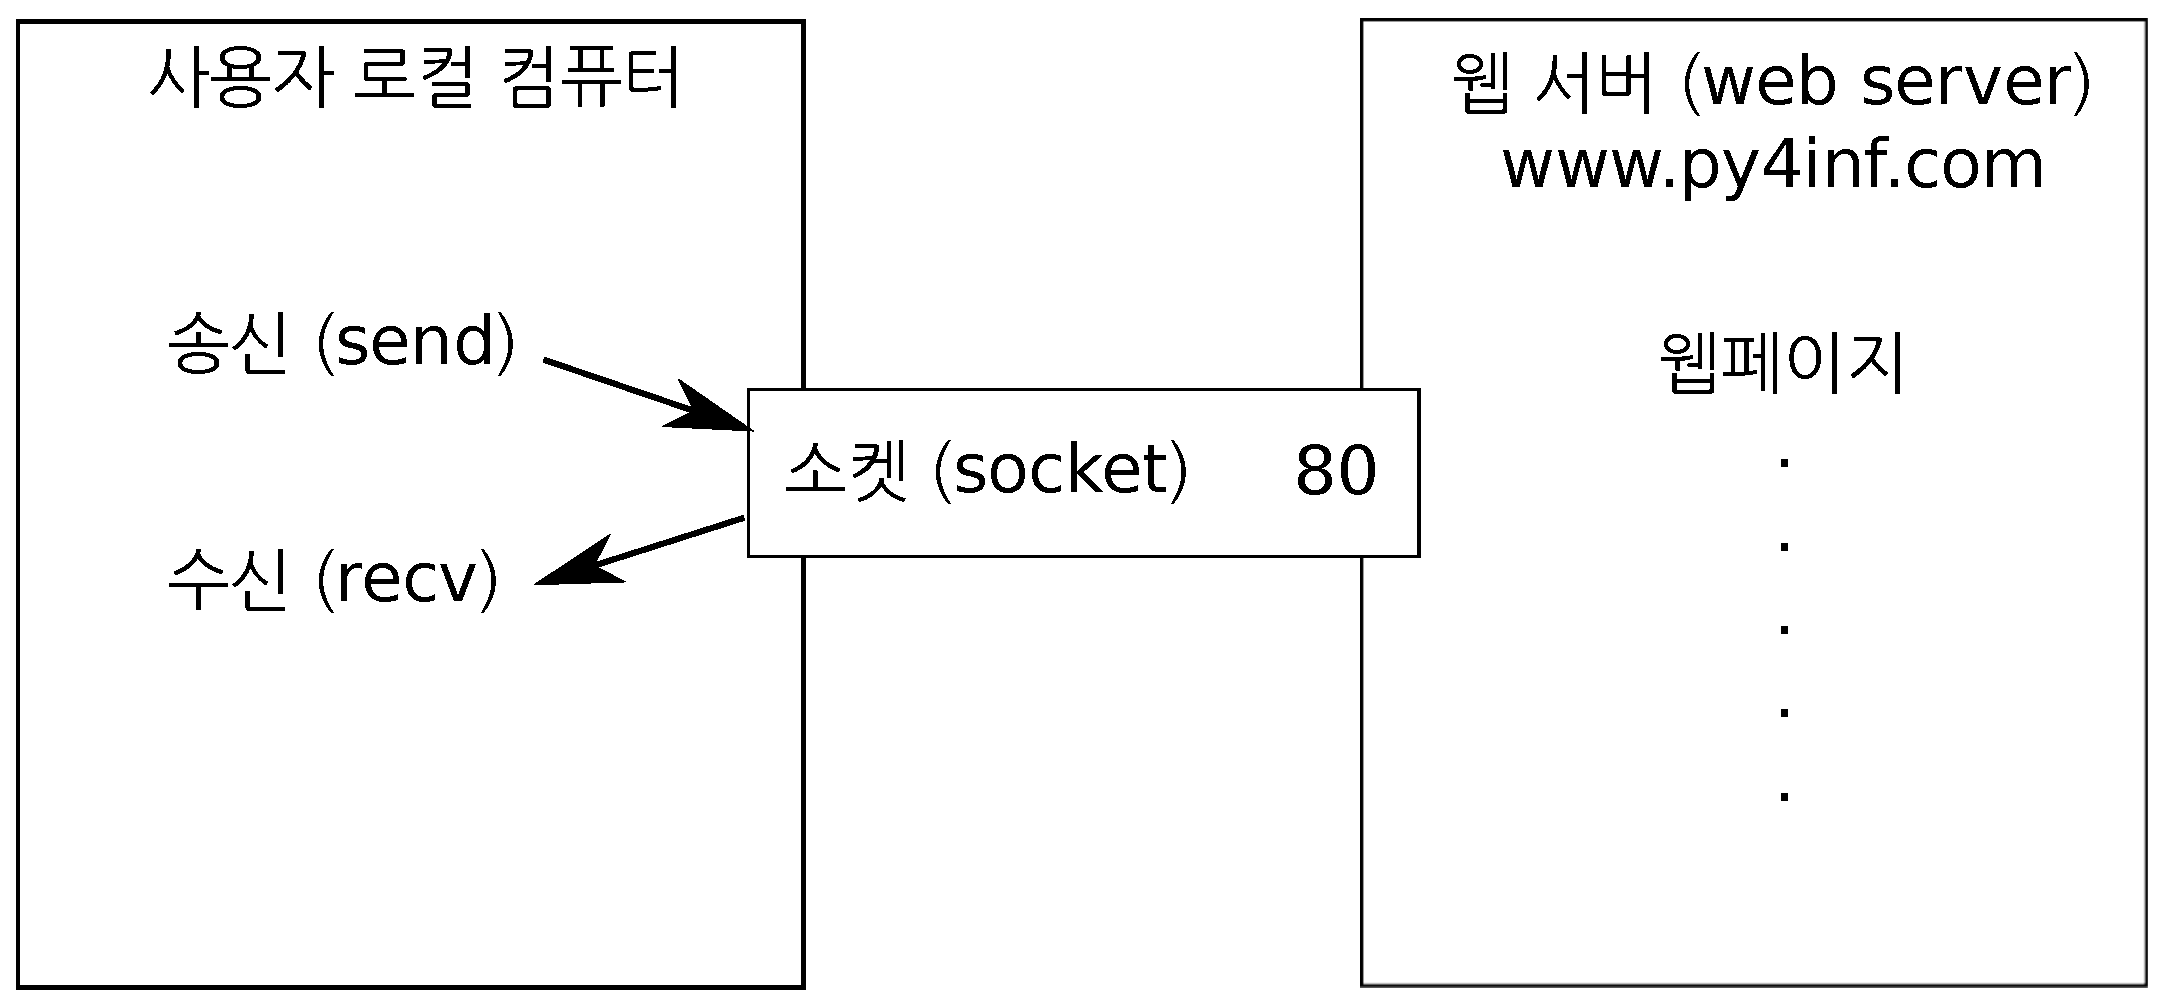
\includegraphics[height=1.50in]{figs2/socket.eps}}
\afterfig

공백 라인을 보내자 마자, 512 문자 덩어리의 데이터를 소켓에서 받아 더 이상 읽을 데이터가 없을 때까지(즉, recv() 빈 문자열을 반환한다.)데이터를 출력하는 루프를 작성한다.

프로그램 실행결과 다음을 얻을 수 있다.

\beforeverb
\begin{verbatim}
HTTP/1.1 200 OK
Date: Sun, 14 Mar 2010 23:52:41 GMT
Server: Apache
Last-Modified: Tue, 29 Dec 2009 01:31:22 GMT
ETag: "143c1b33-a7-4b395bea"
Accept-Ranges: bytes
Content-Length: 167
Connection: close
Content-Type: text/plain

But soft what light through yonder window breaks
It is the east and Juliet is the sun
Arise fair sun and kill the envious moon
Who is already sick and pale with grief
\end{verbatim}
\afterverb
%

출력물은 웹서버가 문서를 서술하기 위해서 보내는 헤더(header)로 시작한다.
예를 들어, {\tt Content-Type } 헤더는 문서가 일반 텍스트 문서({\tt text/plain})임을 표기한다.

서버가 헤더를 보낸 후에 빈 라인을 추가해서 헤더의 끝임을 표기하고 나서 실제 파일{\tt romeo.txt}을 보낸다.

이 예제를 통해서 소켓을 통해서 저수준(low-level) 네트워크 연결을 어떻게 하는지 확인할 수 있다.

소켓을 사용해서 웹서버, 메일 서버 혹은 다른 종류의 서버와 통신할 수 있다.
필요한 것은 프로토콜을 기술하는 문서를 찾고 프로토콜에 따라 데이터를 주고 받는 코드를 작성하는 것이다.

하지만, 가장 흔히 사용하는 프로토콜은 HTTP (즉, 웹) 프로토콜이기 때문에, 파이썬은 웹상에서 데이터나 문서를 검색하기 위해서
HTTP 프로토컬을 지원하기 위해서 특별히 설계된 라이브러리가 있다.


\section{HTTP를 통해서 이미지 가져오기}

\index{urllib!image}
\index{image!jpg}
\index{jpg}

상기 예제에서 파일의 새줄(newline)을 가진 일반 텍스트 파일을 가져와서, 프로그램이 동작할 때 화면상에 데이터를 단순히 복사했다.
HTTP를 사용하여 이미지를 가져오는 비슷한 프로그램을 작성할 수 있다. 프로그램 실행 시에 화면에 데이터를 복사하는 대신에,
문자열로 데이터를 쌓고, 다음과 같이 헤더를 잘라내고 나서 파일에 이미지 데이터를 저장한다. 

\beforeverb
\begin{verbatim}
import socket
import time

mysock = socket.socket(socket.AF_INET, socket.SOCK_STREAM)
mysock.connect(('www.py4inf.com', 80))
mysock.send('GET http://www.py4inf.com/cover.jpg HTTP/1.0\n\n')


count = 0
picture = "";
while True:
    data = mysock.recv(5120)
    if ( len(data) < 1 ) : break
    # time.sleep(0.25)
    count = count + len(data)
    print len(data),count
    picture = picture + data

mysock.close()

# Look for the end of the header (2 CRLF)
pos = picture.find("\r\n\r\n");
print 'Header length',pos
print picture[:pos]

# Skip past the header and save the picture data
picture = picture[pos+4:]
fhand = open("stuff.jpg","wb")
fhand.write(picture);
fhand.close()
\end{verbatim}
\afterverb
%

프로그램을 실행하면, 다음과 같은 출력을 생성한다.

\beforeverb
\begin{verbatim}
$ python urljpeg.py 
2920 2920
1460 4380
1460 5840
1460 7300
...
1460 62780
1460 64240
2920 67160
1460 68620
1681 70301
Header length 240
HTTP/1.1 200 OK
Date: Sat, 02 Nov 2013 02:15:07 GMT
Server: Apache
Last-Modified: Sat, 02 Nov 2013 02:01:26 GMT
ETag: "19c141-111a9-4ea280f8354b8"
Accept-Ranges: bytes
Content-Length: 70057
Connection: close
Content-Type: image/jpeg
\end{verbatim}
\afterverb
%
{\tt Content-Type } 헤더가 문선의 본문이 이미지({\tt image/jpeg})를 나타내는 것을 볼 수 있다.
프로그램이 완료되면, 이미지 뷰어로 {\tt stuff.jpg} 파일을 열어서 이미지 데이터를 볼 수 있다.

프로그램을 실행하면, {\tt recv()} 메쏘드를 호출할 때 마다 5120 문자를 얻지 못하는 것을 볼 수 있다.
{\tt recv()} 호출하는 매 순간 웹서버에서 네트워크로 전송되는 가능한 많은 문자를 받게 된다. 
5120 문자까지 요청을 매번 하지만, 1460 혹은 2920 문자를 얻는다. 

결과값은 네트워크 속도에 따라 달라질 수 있다. {\tt recv()} 메쏘드의 마지막 호출에는 스트림 끝에 1681 바이트만 받았고,
{\tt recv()} 다음 호출에는 0 길이 문자열을 얻게 되어서 서버가 소켓의 마지막에 {\tt close()}를 호출하고 
더이상 데이터가 없다는 것을 알려준다.

\index{time}
\index{time.sleep}

주석처리한 {\tt time.sleep()}을 풀어줌으로써 {\tt recv()} 연속 호출을 늦출 수 있다.
이런 방식으로 매 호출 후에 0.25초 기다리게 함으로서 서버가 먼저 도축할 수 있어서 더 많은 데이터를 
사용자가 {\tt recv()} 호출하기 전에 보낼 수가 있다.
지연을 넣어서 프로그램을 다시 실행하면 다음과 같다.

\beforeverb
\begin{verbatim}
$ python urljpeg.py 
1460 1460
5120 6580
5120 11700
...
5120 62900
5120 68020
2281 70301
Header length 240
HTTP/1.1 200 OK
Date: Sat, 02 Nov 2013 02:22:04 GMT
Server: Apache
Last-Modified: Sat, 02 Nov 2013 02:01:26 GMT
ETag: "19c141-111a9-4ea280f8354b8"
Accept-Ranges: bytes
Content-Length: 70057
Connection: close
Content-Type: image/jpeg
\end{verbatim}
\afterverb
%

{\tt recv()} 호출에 처음과 마지막을 제외하고, 매번 새로운 데이터를 요청할 때마다 이제는 5120 문자를 얻는다. 

서버 {\tt send()} 요청과 응용프로그램 {\tt recv()} 요청 사이에 버퍼가 있다.
프로그램에 지연을 넣어 실행하게 될 때, 어느 지점엔가 서버가 소켓의 버퍼를 채우고 응용프로그램이 버퍼를 비울 때까지
잠시 멈춰야 된다. 보내는 응용프로그램 혹은 받는 응용프로그램을 멈추는 행위를 ''흐름 제어(flow control)''이라고 한다.

\index{flow control}

\section{{\tt urllib} 사용하여 웹페이지 가져오기}

수작업으로 소켓 라이브러리를 사용하여 HTTP로 데이터를 보내거나 받을 수 있지만,
{\tt urllib} 라이브러리를 사용하여 파이썬에서 동일한 작업을 수행하는 좀더 간편한 방식이 있다.

{\tt urllib}을 사용하여 파일처럼 웹페이지를 다룰 수가 있다.
단순하게 어느 웹페이지를 가져오늘 것인지만 지정하면 {\tt urllib} 라이브러리가 모든 HTTP 프로토콜과 헤더관련 사항을 처리해 준다.

{\tt urllib}를 사용하여 웹으로부터 {\tt romeo.txt} 파일을 읽는 상응하는 코드는 다음과 같다.

\beforeverb
\begin{verbatim}
import urllib

fhand = urllib.urlopen('http://www.py4inf.com/code/romeo.txt')
for line in fhand:
   print line.strip()
\end{verbatim}
\afterverb
%

{\tt urllib.urlopen}으로 웹페이지를 열게 되면, 파일처럼 다룰 수 있고 {\tt for} 루프를 사용하여 데이터를 읽을 수 있다.

프로그램을 실행하면, 파일 내용의 출력만을 볼 수 있다. 헤더정보가 여전히 보내지지만, {\tt urllib} 코드가 헤더를 받아 내부적으로 처리하고,
단지 데이터만 사용자에게 반환한다.

\beforeverb
\begin{verbatim}
But soft what light through yonder window breaks
It is the east and Juliet is the sun
Arise fair sun and kill the envious moon
Who is already sick and pale with grief
\end{verbatim}
\afterverb
%

예제로, {\tt romeo.txt} 데이터를 가져와서 파일의 각 단어의 빈도를 계산하는 프로그램을 다음과 같이 작성할 수 있다.

\beforeverb
\begin{verbatim}
import urllib

counts = dict()
fhand = urllib.urlopen('http://www.py4inf.com/code/romeo.txt')
for line in fhand:
    words = line.split()
    for word in words:
        counts[word] = counts.get(word,0) + 1   
print counts
\end{verbatim}
\afterverb
%

다시 한번, 웹페이지를 열게 되면, 로컬 파일처럼 웹페이지를 읽을 수 있다.

\section{HTML 파싱과 웹 스크래핑}

\index{web!scraping}
\index{parsing HTML}

파이썬 {\tt urllib} 활용하는 흔한 사례는 웹 {\bf 스크래핑(scraping)}이다.
웹 스크래핑은 웹브라우저를 가장하여 웹페이지를 가져와서 페이지 내부의 데이터를 살펴보고 패턴을 찾은 프로그램을 작성하는 것이다.
예로, 구글같은 검색엔진은 웹 페이지의 소스를 찾아서 다른 페이지로의 링크를 추출하고, 다른 페이지를 가져와서 링크를 추출하는 일을 반복한다.
이러한 기법으로 구글은 웹상의 거의 모든 페이지를 {\bf 거미(spiders)}줄처럼 연결한다.

구글은 또한 다른 페이지로 연결되는 링크의 빈도를 사용하여 얼마나 중요한 페이지인지를 측정하고 
페이지가 검색결과에 얼마나 높이 나타낸다.

\section{정규 표현식 사용 HTML 파싱하기}

HTML을 파싱하는 한가지 간단한 방식은 정규 표현식을 사용하여 특정한 패턴과 매칭하는 부속문자열을 반복적으로 찾아 추출하는 것이다.

여기 간단한 웹페이지가 있다.

\beforeverb
\begin{verbatim}
<h1>The First Page</h1>
<p>
If you like, you can switch to the
<a href="http://www.dr-chuck.com/page2.htm">
Second Page</a>.
</p>
\end{verbatim}
\afterverb
%

상기 웹페이지에서 링크를 찾아 추출하는 적격의 정규표현식을 다음과 같이 구성할 수 있다.

\beforeverb
\begin{verbatim}
href="http://.+?"
\end{verbatim}
\afterverb
%

작성된 정규 표현식은 ``href="http://''로 시작하고, 하나 혹은 이상의 ``.+?'' 문자를 가지고 큰 따옴표를 가진 문자열을 찾는다.
``.+?''에 물음표는 매칭이 ''욕심(greedy)'' 방식보다 ''비욕심(non-greedy)'' 방식으로 수행됨을 나타낸다. 
비욕심 매칭방식은 가능한 가장 작게 매칭되는 문자열을 찾는 방식이고, 욕심 방식은 가능한 가장 크게 매칭되는 문자열을 찾는 방식이다.

\index{greedy}
\index{non-greedy}

추출하고자 하는 문자열의 어느부분인지를 표기하기 위해서 정규 표현식에 괄호를 추가하여 다음과 같이 프로그램을 작성한다.

\index{regex!parentheses}
\index{parentheses!regular expression}

\beforeverb
\begin{verbatim}
import urllib
import re

url = raw_input('Enter - ')
html = urllib.urlopen(url).read()
links = re.findall('href="(http://.*?)"', html)
for link in links:
    print link
\end{verbatim}
\afterverb
%

{\tt findall} 정규 표현식 메쏘드는 정규 표현식과 매칭되는 모든 문자열 리스트를 추출하여 큰 따옴표 사이에 링크 텍스트만을 반한한다.

프로그램을 실행하면, 다음 출력을 얻게된다.

\beforeverb
\begin{verbatim}
python urlregex.py 
Enter - http://www.dr-chuck.com/page1.htm
http://www.dr-chuck.com/page2.htm

python urlregex.py 
Enter - http://www.py4inf.com/book.htm
http://www.greenteapress.com/thinkpython/thinkpython.html
http://allendowney.com/
http://www.py4inf.com/code
http://www.lib.umich.edu/espresso-book-machine
http://www.py4inf.com/py4inf-slides.zip
\end{verbatim}
\afterverb
%

정규 표현식은 HTML이 예측가능하고 잘 구성된 경우에 멋지게 작동한다.
하지만, ''망가진'' HTML 페이지가 많아서, 정규 표현식만을 사용하는 솔류션은 유효한 링크를 놓치거나 잘못된 데이터를 찾게 되는 것으로 끝날 수 있다.

이 문제는 강건한 HTML 파싱 라이브러리를 사용해서 해결될 수 있다.

\section{BeautifulSoup 사용한 HTML 파싱}
\index{BeautifulSoup}

HTML을 파싱하여 페이지에서 데이터를 추출할 수 있는 파이썬 라이브러리는 많이 있다.
각각의 라이브러리는 강점과 약점이 있어서 사용자 필요에 따라 취사선택하여야 한다.

예로, 간단하게 HTML 입력을 파싱하여 {\bf BeautifulSoup} 라이브러리를 사용하여 링크를 추출할 것이다.
다음 웹사이트에서 BeautifulSoup 코드를 다운로드 받아 설치할 수 있다.

\url{www.crummy.com}

BeautifulSoup 라이브러리를 다운로드 받아 ''설치''하거나 {\tt BeautifulSoup.py} 파일을 응용프로그램과 동일한 폴더에 놓을 수 있다.

HTML이 XMX 처럼 보이고 몇몇 페이지는 XML로 되도록 꼼꼼하게 구축되었지만, 대부분의 HTML은 통상 잘못 구축되어서 XML 파서가 HTML 전체 페이지를 
잘못 구성된 것으로 거부한다. BeautifulSoup 라이브러리는 결점 많은 HTML 페이지에 내성이 있어서 사용자가 필요로하는 데이터를 쉽게 추출할 수 있게 한다.

{\tt urllib}를 사용하여 페이지를 읽어들이고, {\tt BeautifulSoup}를 사용하여 앵커 태그 ({\tt a})로 {\tt href} 속성을  추출합니다.

\index{BeautifulSoup}
\index{HTML}
\index{parsing!HTML}

\beforeverb
\begin{verbatim}
import urllib
from BeautifulSoup import *

url = raw_input('Enter - ')
html = urllib.urlopen(url).read()
soup = BeautifulSoup(html)

# Retrieve all of the anchor tags
tags = soup('a')
for tag in tags:
   print tag.get('href', None)
\end{verbatim}
\afterverb
%

프로그램이 웹 주소를 입력받고, 웹페이지를 열고, 데이터를 읽어서 BeautifulSoup 파서에 전달하고,
그리고 나서 모든 앵커 태그를 불러와서 각 태그에 {\tt href} 속성을 출력한다.

프로그램을 실행하면, 아래와 같다.

\beforeverb
\begin{verbatim}
python urllinks.py 
Enter - http://www.dr-chuck.com/page1.htm
http://www.dr-chuck.com/page2.htm

python urllinks.py 
Enter - http://www.py4inf.com/book.htm
http://www.greenteapress.com/thinkpython/thinkpython.html
http://allendowney.com/
http://www.si502.com/
http://www.lib.umich.edu/espresso-book-machine
http://www.py4inf.com/code
http://www.pythonlearn.com/
\end{verbatim}
\afterverb
%

BeautifulSoup을 사용하여 다음과 같이 각 태그의 다양한 부분을 뽑아낼 수 있다.

\beforeverb
\begin{verbatim}
import urllib
from BeautifulSoup import *

url = raw_input('Enter - ')
html = urllib.urlopen(url).read()
soup = BeautifulSoup(html)

# Retrieve all of the anchor tags
tags = soup('a')
for tag in tags:
   # Look at the parts of a tag
   print 'TAG:',tag
   print 'URL:',tag.get('href', None)
   print 'Content:',tag.contents[0]
   print 'Attrs:',tag.attrs
\end{verbatim}
\afterverb
%

상기 프로그램은 다음을 출력합니다.

\beforeverb
\begin{verbatim}
python urllink2.py 
Enter - http://www.dr-chuck.com/page1.htm
TAG: <a href="http://www.dr-chuck.com/page2.htm">
Second Page</a>
URL: http://www.dr-chuck.com/page2.htm
Content: [u'\nSecond Page']
Attrs: [(u'href', u'http://www.dr-chuck.com/page2.htm')]
\end{verbatim}
\afterverb
%

HTML을 파상하는데 BeautifulSoup이 가진 강력한 기능을 예제로 보여줬습니다.
좀더 자세한 사항은 \url{www.crummy.com} 에서 문서와 예제를 살펴보세요.

\section{urllib을 사용하여 바이너리 파일 읽기}

이미지나 비디오 같은 텍스트가 아닌 (혹은 바이너리)파일을 가져올 때가 종종 있다.
이런 파일의 데이터는 일반적으로 출력하는 것은 유용하지 않다. 하지만, {\tt urllib}을 사용하여,
하드 디스크의 로컬 파일에 URL 사본을 쉽게 만들 수 있다.

\index{binary file}

패턴은 URL을 열고, {\tt read}를 사용해서 문서 전체의 내용을 다운로드하여 문자열 변수({\tt img})에 다운로드하고,
그 정보를 다음과 같이 로컬 파일에 쓴다.

\beforeverb
\begin{verbatim}
img = urllib.urlopen('http://www.py4inf.com/cover.jpg').read()
fhand = open('cover.jpg', 'w')
fhand.write(img)
fhand.close()
\end{verbatim}
\afterverb
%

작성한 프로그램은 네트워크로 모든 데이터를 한번에 읽어서 컴퓨터 주기억장치의 {\tt img} 변수에 저장하고,
{\tt cover.jpg} 파일을 열어 디스크에 데이터를 쓴다. 이 방식은 파일의 크기가 사용자 컴퓨터의 메모리 크기보다 작으면 정상적으로 작동한다.

하지만, 큰 오디오 혹은 비디오 파일이라면, 상기 프로그램은 멈추거나 사용자 컴퓨터가 메모리가 부족할 때 극단적으로 느려질 수 있다.
메모리 부족을 피하기 위해서, 데이터를 블럭 혹은 버퍼로 가져오고 다음 블럭을 가져오기 전에 디스크에 각각의 브럭을 쓴다.
이런 방식으로 사용자가 가진 모든 메모리를 사용하지 않고 임의 크기의 파일을 읽어올 수 있다.

\beforeverb
\begin{verbatim}
import urllib

img = urllib.urlopen('http://www.py4inf.com/cover.jpg')
fhand = open('cover.jpg', 'w')
size = 0
while True:
    info = img.read(100000)
    if len(info) < 1 : break
    size = size + len(info)
    fhand.write(info)

print size,'characters copied.'
fhand.close()
\end{verbatim}
\afterverb
%

상기 예제에서, 한번에 100,000 문자만 읽어 오고, 웹에서 다음 100,000 문자를 가져오기 전에 {\tt cover.jpg} 파일에 읽어온 문자를 쓴다.

프로그램 실행 결과는 다음과 같다.

\beforeverb
\begin{verbatim}
python curl2.py 
568248 characters copied.
\end{verbatim}
\afterverb
%

UNIX 혹은 매킨토시 컴퓨터를 가지고 있다면, 다음과 같이 이러한 동작을 수행하는 명령어가 운영체제에 내장되어 있다.

\index{curl}

\beforeverb
\begin{verbatim}
curl -O http://www.py4inf.com/cover.jpg
\end{verbatim}
\afterverb
%

{\tt curl}은 ``copy URL''의 단축 명령어로 두 예제는 {\tt curl} 명령어와 비슷한 기능을 구현해서, 
\url{www.py4inf.com/code} 사이트에 {\tt curl1.py}, {\tt curl2.py} 이름으로 올라가 있다.
동일한 작업을 좀더 효과적으로 수행하는 {\tt curl3.py} 샘플 프로그램도 있어서 실질적으로 작성하는 프로그램에 이런한 패턴을 이용하여 구현할 수 잇다.

\section{용어정의}

\begin{description}

\item[BeautifulSoup:] 파이썬 라이브러리로 HTML 문서를 파싱하고 
브라우저가 일반적으로 생략하는 HTML의 불완전한 부분을 보정하여 HTML 문서에서 데이터를 추출한다.
\url{www.crummy.com} 사이트에서 BeautifulSoup 코드를 다운로드 받을 수 있다.

\index{BeautifulSoup}

\item[포트(port):] 서버에 소켓 연결을 할 때, 사용자가 어느 응용프로그램을 연결하는지 나타내는 숫자.
예로, 웹 트래픽은 통상 80 포트, 전자우편은 25 포트를 사용한다.

\index{port}

\item[스크랩(scrape):] 프로그램이 웹브라우저를 가장하여 웹페이지를 가져오고 웹 페이지의 내용을 검색한다.
종종 프로그램이 한 페이지의 링크를 따라 다른 페이지를 찾아서 웹페이지 네트워크 혹은 소셜 네트워크 전체를 훑을 수 있다.

\index{socket}

\item[소켓(socket):] 두 응용프로그램 사이의 네트워크 연결. 두 응용프로그램은 양 방향으로 데이터를 주고 받는다.
\index{socket}

\item[스파이더(spider):] 검색 색인을 구축하기 위해서 한 웹페이지에서 그 페이지에 링크된 모든 페이지를 가져오기를 반복하여
거의 모든 인터넷의 모든 페이지를 가져오기 위해서 사용하는 검색엔진 행동.
\index{spider}

\end{description}

\section{연습문제}

\begin{ex}
소켓 프로그램 {\tt socket1.py}을 변경하여 임의의 웹페이지를 읽을 수 있도록 URL을 사용자가 입력하도록 바꾸세요.
{\tt split('/')}을 사용하여 URL을 컴포턴트로 쪼개서 소켓 {\tt connect} 호출에 대해 호스트 명을 추출할 수 있다.
사용자가 적절하지 못한 형식 혹은 존재하지 않는 URL을 입력하는 경우를 다룰 수 있도록 {\tt try}, {\tt except}를 사용하여 오류 검사기능을 추가하세요.
\end{ex}

\begin{ex}
소켓 프로그램을 변경하여 받은 문자갯수를 세고 3000 문자를 출력한 후에 더이상의 텍스트를 출력을 멈추게 하세요.
프로그램은 전체 문서를 가져와야 하고 전체 문자 갯수를 세고, 문서 마지막에 문자 갯수를 출력해야 합니다.
\end{ex}

\begin{ex}
{\tt urllib}을 사용하여 앞의 예제를 반복하세요. (1) 사용자가 입력한 URL에서 문서 가져오기
(2) 3000 문자까지 화면에 보여주기 (3) 문서의 전체 문자 갯수 세기.
이 예제에서 헤더에 대해서는 걱정하지 말고, 단지 문서 본문에서 첫 3000 문자만 화면에 출력하세요.
\end{ex}

\begin{ex} {\tt urllinks.py} 프로그램을 변경하여 가져온 HTML 문서에서 문단 (p) 태그를 추출하고
프로그램의 출력물로 문단 숫자를 세고 화면에 출력하세요. 문단 텍스트를 화면에 출력하지 말고 단지 숫자만 셉니다.
작성한 프로그램을 작은 웹페이지 뿐만 아니라 조금 큰 웹 페이지에도 테스트해 보세요.
\end{ex}

\begin{ex}
(고급) 소켓 프로그램을 변경하여 헤더와 빈 라인을 받은 후에 데이터만 보여지게 하세요.
{\tt recv}는 라인이 아니라 문자(새줄(newline)과 모든 문자)를 받는다는 것을 기억하세요.
\end{ex}



%% The contents of this file is 
% Copyright (c) 2009-  Charles R. Severance, All Righs Reserved

\chapter{웹서비스 사용하기}
프로그램을 사용하여 HTTP상에서 문서를 가져오고 파싱하는 것이 쉽게 되면, 다른 프로그램에서 
활용되도록 특별히 설계된 문서(즉, 브라우져에서 HTML로 보여지지 않는 것)를 생성하는 방법을 개발하는 것은 오래 걸리지 않는다.

웹상에서 데이터를 교환할 때 두 가지 일반적인 형식이 있다.
XML(``eXtensible Markup Language'')은 오랜 기간 사용되어져 왔고 문서형식 데이터를 교환하는데 적절하다.
딕셔너리, 리스트 혹은 다른 내부 정보를 프로그램으로 서로 교환할 때, JSON(JavaScript Object Notation, \url{www.json.org})을 사용한다. 두 가지 형식에 대해서 살펴볼 것이다.

\section{XML(eXtensible Markup Language)}
XML은 HTML과 매우 유사하지만, XML은 좀더 HTML보다 구조화되었다.
여기 XML 문서 샘플이 있다.

\beforeverb
\begin{verbatim}
<person>
  <name>Chuck</name>
  <phone type="intl">
     +1 734 303 4456
   </phone>
   <email hide="yes"/>
</person>
\end{verbatim}
\afterverb
%

종종 XML문서를 나무 구조로 생각하는 것이 도움이 된다. 최상단 {\tt person} 태그가 있고
{\tt phone} 같은 다른 태그는 부모 노드의 \emph{자식(children)} 노드로 그려진다.

\beforefig
\centerline{\includegraphics[height=1.50in]{figs2/xml-tree.eps}}
\afterfig

\section{XML 파싱}

\index{ElementTree}
\index{ElementTree!fromstring}
\index{ElementTree!find}

다음은 XML을 파싱하고 XML에서 데이터 요소를 추출하는 간단한 응용프로그램이다.

\beforeverb
\begin{verbatim}
import xml.etree.ElementTree as ET

data = '''
<person>
  <name>Chuck</name>
  <phone type="intl">
     +1 734 303 4456
   </phone>
   <email hide="yes"/>
</person>'''

tree = ET.fromstring(data)
print 'Name:',tree.find('name').text
print 'Attr:',tree.find('email').get('hide')
\end{verbatim}
\afterverb
%

{\tt fromstring}을 호출하여 XML 문자열 표현식을 XML 노드의 '나무(tree)'로 변환한다.
XML이 나무구조로 되어 있을 때, XML에서 데이터의 일부분을 추출하기 위해서 호출할 일련의 메쏘드가 있다.

{\tt find} 함수는 XML 나무를 훑어서 특정 태그와 매칭되는 {\bf 노드(node)}를 검색한다. 
각 노드는 텍스트, 속성(즉, hide 같은), 그리고 ''자식(child)'' 노드로 구성된다. 각 노드는 노드 나무의 최상단이 될 수 있다.

\beforeverb
\begin{verbatim}
Name: Chuck
Attr: yes
\end{verbatim}
\afterverb
%

{\tt ElementTree}같은 XML 파서를 사용하는 것은 잇점이 있는데 상기 예제의 XML은 매우 간단하지만,
적합한 XML에 대한 많은 규칙이 있고, {\tt ElementTree}를 사용해서 XML 구문 규칙에 얽매이지 않고 XML에서
데이터를 추출할 수 있다.

\section{노드 반복하기}

\index{ElementTree!findall}
\index{ElementTree!get}

종종 XML은 다중 노드를 가지고 있어서 모든 노드를 처리하기 위해서 루프를 작성할 필요가 있다.
다음 프로그램에서 모든 {\tt user} 노드를 루프로 반복한다.

\beforeverb
\begin{verbatim}
import xml.etree.ElementTree as ET

input = '''
<stuff>
    <users>
        <user x="2">
            <id>001</id>
            <name>Chuck</name>
        </user>
        <user x="7">
            <id>009</id>
            <name>Brent</name>
        </user>
    </users>
</stuff>'''

stuff = ET.fromstring(input)
lst = stuff.findall('users/user')
print 'User count:', len(lst)

for item in lst:
    print 'Name', item.find('name').text
    print 'Id', item.find('id').text
    print 'Attribute', item.get('x')
\end{verbatim}
\afterverb
%

{\tt findall} 메쏘드는 XML 나무의 {\tt user} 구조를 표현하는 파이썬 리스트의 하위 나무를 가져온다.
그리고 나서, {\tt for} 루프를 작성해서 {\tt user} 노드의 각 값을 확인하고 {\tt name}, {\tt id} 텍스트 요소와 
{\tt user} 노드에서 {\tt x} 속성을 출력한다.

\beforeverb
\begin{verbatim}
User count: 2
Name Chuck
Id 001
Attribute 2
Name Brent
Id 009
Attribute 7
\end{verbatim}
\afterverb
%

\section{JSON(JavaScript Object Notation)}
\index{JSON}
\index{JavaScript Object Notation}

JSON 형식은 자바스크립트 언어에서 사용되는 개체와 배열 형식에서 영감을 얻었다.
하지만 파이썬이 자바스크립트 이전에 개발되어서 딕셔너리와 리스트의 파이썬 구문이 JSON 구문에 영향을 주었다.
그래서 JSON 포맷이 거의 파이썬의 리스트와 딕셔너리의 조합과 일치한다. 

상기 간단한 XML에 대략 상응하는 JSON으로 작성한 것이 다음에 있다.

\beforeverb
\begin{verbatim}
{
  "name" : "Chuck",
  "phone" : {
    "type" : "intl",
    "number" : "+1 734 303 4456"
   },
   "email" : {
     "hide" : "yes"
   }
}
\end{verbatim}
\afterverb
%

몇가지 차이점에 주목하세요. 첫째로 XML에서는 ''phone'' 태그에 ''intl''같은 속성을 추가할 수 있다.
JSON에서는 단지 키-밸류 페어(key-value pair)다. 또한 XML ''person'' 태그는 사라지고 중괄호 세트로 대체되었다.

일반적으로 JSON 구조가 XML보다 간단하다. 왜냐하면, JSON이 XML보다 적은 역량을 보유하기 때문이다.
하지만 JSON이 딕셔너리와 리스트의 조합에 {\em 직접} 매핑된다는 장점이 있다.
그리고, 거의 모든 프로그래밍 언어가 파이썬 딕셔너러와 리스트에 상응하는 것을 가지고 있어서,
JSON이 두 협업 프로그램이 데이터를 교환하는데 매우 자연스러운 형식이 된다.

XML에 비해서 상대적으로 단순함으로써, JSON은 응용프로그램 간의 거의 모든 데이터를 교환하는데 있어
빠르게 선택되고 있다. 

\section{JSON 파싱하기}
딕셔너리(개체)와 리스트를 중첩함으로써 JSON을 생성한다. 이번 예제에서,
각 user가 딕셔너리로 키-밸류 페어(key-value pair)인 user 리스트를 표현한다. 그래서 리스트 딕셔너리가 있다.

다음 프로그램에서 내장된 {\bf json} 라이브러리를 사용하여 JSON을 파싱하여 데이터를 읽어온다.
이것을 XML과 상응하는 데이터, 코드와 비교해 보세요. JSON은 조금 덜 자세해서 사전에 미리 리스트를 가져올 것이고, user 리스트가 있고 각 user는 키-밸류 페어 집합임을 알 수 있다. JSON은 좀더 간략(장점)하고 하지만 
좀더 덜 서술적(단점)이다. 

\beforeverb
\begin{verbatim}
import json

input = '''
[
  { "id" : "001",
    "x" : "2",
    "name" : "Chuck"
  } ,
  { "id" : "009",
    "x" : "7",
    "name" : "Chuck"
  } 
]'''

info = json.loads(input)
print 'User count:', len(info)

for item in info:
    print 'Name', item['name']
    print 'Id', item['id']
    print 'Attribute', item['x']
\end{verbatim}
\afterverb
%

JSON과 XML에서 데이터를 추출하는 코드를 비교하면, 
{\bf json.loads()} 에서 파이썬 리스트를 얻고,
{\bf for} 루프로 훑고, 리스트 내부의 각 항목은 파이썬 딕셔너리로
각 user의 다양한 정보를 추출하기 위해서 파이썬 인덱스 연산자를 사용한다. 
JSON을 파싱하면, 네이티브 파이썬 개체와 구조가 생성된다.
반환된 데이터가 단순히 네이티브 파이썬 구조체이기 때문에, 파싱된 JSON을 활용하는데
JSON 라이브러리를 사용할 필요는 없다. 
 
프로그램 출력은 정확하게 상기 XML 버젼과 동일한다.

\beforeverb
\begin{verbatim}
User count: 2
Name Chuck
Id 001
Attribute 2
Name Brent
Id 009
Attribute 7
\end{verbatim}
\afterverb
%

일반적으로 웹서비스에 대해서 XML에서 JSON으로 가는 산업 경향이 뚜렷하다.
JSON이 좀더 간단하고 이미 프로그래밍 언어에서 갖고 있는 네이티브 자료 구조와 직접적으로 매핑되기 때문에
파싱하고 데이터 추출하는 코드는 JSON을 사용할 때 좀더 간단하고 직접적이다.
하지만 XML이 JSON보다 좀더 자기 서술적이고 XML이 강점을 가지는 몇몇 어플리케이션이 있다.
예를 들어, 대부분의 워드 프로세서는 JSON보다는 XML을 사용하여 내부적으로 문서를 저장한다. 

\section{API(Application Program Interfaces, 응용 프로그램 인터페이스)}

이제 HTTP를 사용하여 응용프로그램간에 데이터를 교환하고 XML과 JSON을 사용하여 응용프로그램간에도
복잡한 데이터를 주고 받을 수 있는 방법을 습득했다.

다음 단계는 이들 기법을 사용하여 응용프로그램 간에 ''계약(contract)''을 정의하고 문서화하는 것이다.
응용프로그램-대-응용프로그램 계약의 일반적 명칭은 APIs, {\bf 응용 프로그램 인터페이스(Application Program 
Interfaces)}이다. API를 사용할 때, 일반적으로 하나의 프로그램은 다른 응용 프로그램에서 사용되도록
가능한 서비스 집합을 생성하고 프로그램에서 제공하는 서비스에 접근하도록 API (즉, ''규칙'')를 게시한다.  

프로그램의 기능이 다른 프로그램에서 제공되는 서비스에 접근도 포함되도록 프로그램을 개발 할 때,
이러한 개발 접근법을 SOA, {\bf Service-Oriented Architecture(서비스 지향 아키텍처)}라고 부른다.
SOA가 아닌 접근법은 응용 프로그램이 하니의 독립 응용 프로그램으로 구현에 필요한 모든 코드를 담고 있다.

웹을 사용할 때 SOA의 많은 사례를 찾아 볼 수 있다. 하나의 웹사이트를 방문하여 비행기표, 호텔, 자동차를 단일
사이트에서 예약한다. 호텔관련 데이터는 물론 항공사 컴퓨터에 저장되어 있지 않다.
대신에 항공사 컴퓨터는 호텔 컴퓨터와 계약을 맺어 호텔 데이터를 가져와서 사용자에게 보여준다.
사용자가 항공사 사이트를 통해서 호텔 예약을 동의할 경우, 항공사 사이트는 실제 예약을 하기 위해서
호텔 시스템의 또다른 웹서비스를 사용한다.
전체 트랜젝션에 대해서 카드 결재를 할 때, 여전히 다른 컴퓨터가 프로세스에 물려있다.

\beforefig
\centerline{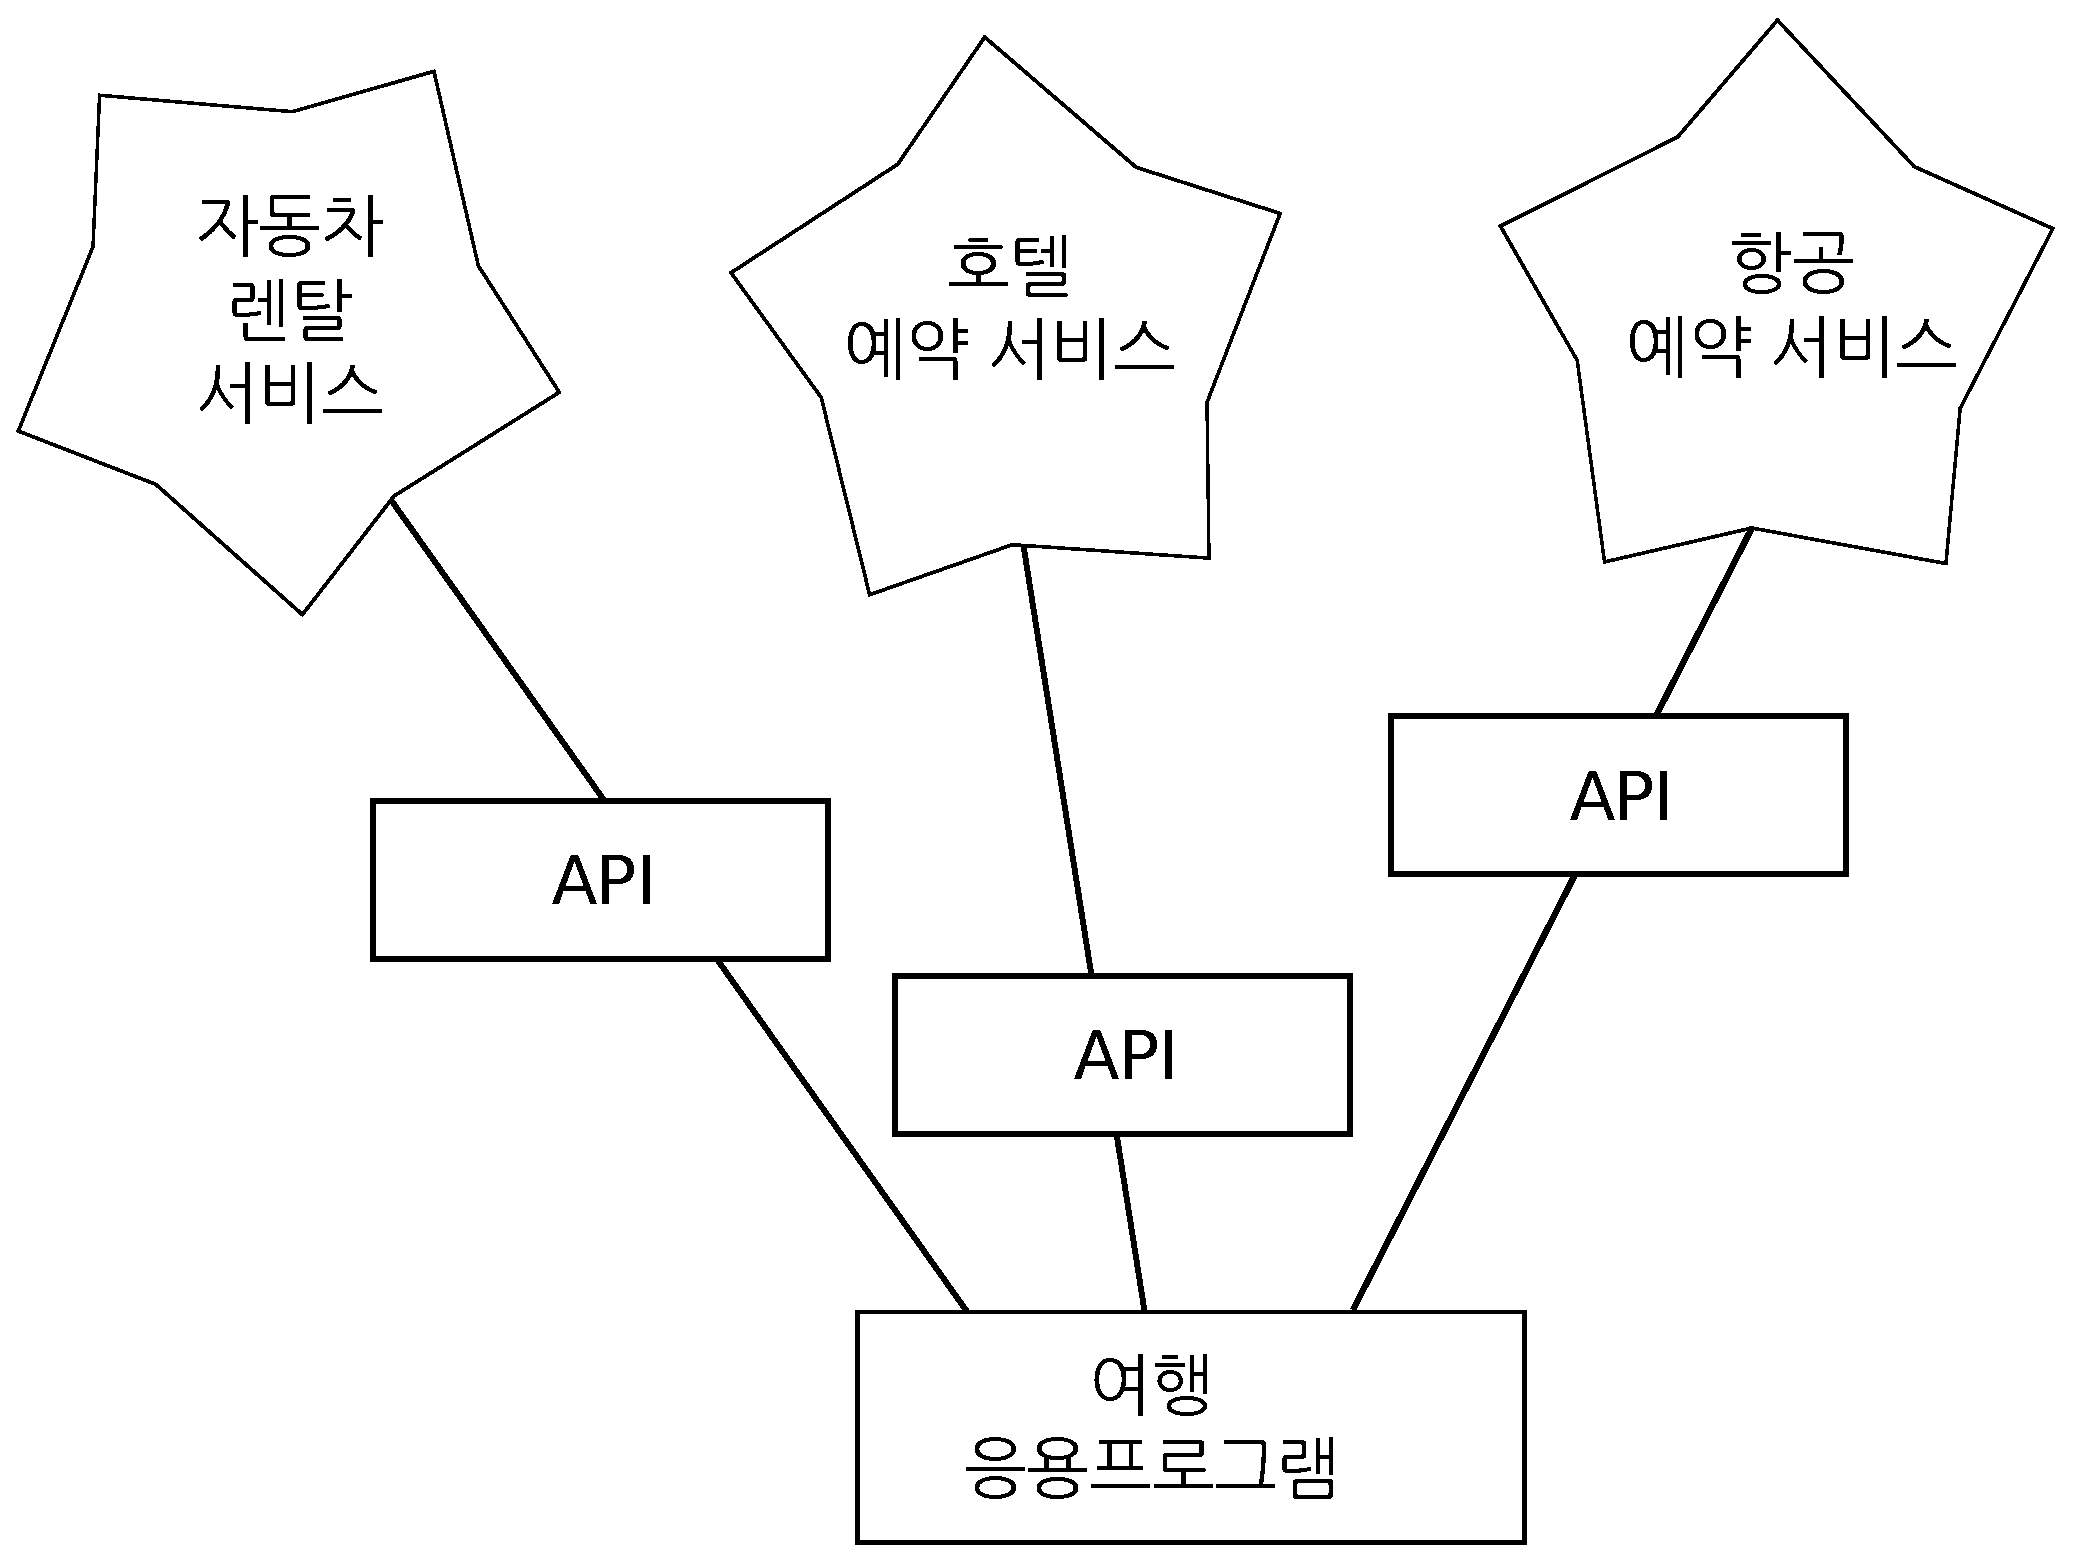
\includegraphics[height=2.50in]{figs2/soa.eps}}
\afterfig

서비스 지향 아키텍쳐는 많은 장점을 지니고 있다. (1) 항상 단 하나의 데이터만 유지관리한다. 
능력 이상으로 예약을 원치않는 호텔  같은 경우에 특히나 중요하다. (2) 데이터 소유자가 
데이터의 사용에 대한 규칙을 정한다. 이러한 장점으로, SOA 시스템은 좋은 성능과 사용자 요구를 만족하기 위해서
주의깊이 설계되어야 한다. 

응응프로그램이 웹상에서 가능한 API 형식의 서비스 집합을 만들 때, {\bf 웹서비스(web services)}라고 부른다.

\section{구글 지오코딩 웹서비스(Google Geocoding Web Service)}
\index{Google}
\index{geocoding}
\index{web service}

구글은 자체적으로 구축한 대용량 지리 정보 데이터베이스를 이용할 수 있게 해주는 훌륭한 웹서비스가 있다.
``Ann Arbor, MI'' 같은 지리적 검색 문자열을 지오코딩 API에 넣으면, 
검색 문자열을 찾아서 지도상에 근처의 주요 지형지물과 함께 최선의 예측치를 보여준다. 

지오코딩 서비스는 무료지만 사용량은 제한되어 있어서, 상업적 응용프로그램에 API를 제한없이 사용할 수는 없다.
하지만, 최종 사용자가 자유형식 입력 박스에 위치정보를 입력하는 설문 데이터가 있다면,
API를 사용하여 데이터를 깔끔하게 정리할 수는데 사용할 수 있다.

{\em When you are using a free API like Google's geocoding API, you need
to be respectful in your use of these resources.  If too many people abuse the
service, Google might drop or significantly curtail its free service.}
\index{rate limiting}

서비스에 대한 온라인 문서를 정독할 수 있지만, 무척 간단해서 브라우저에 다음 URL을 입력함으로써 테스트까지 할 수 있다.

\url{http://maps.googleapis.com/maps/api/geocode/json?sensor=false &address=Ann+Arbor%2C+MI}

URL만 벗겨내고 웹프라우저에 붙여넣기 전에 URL에서 모든 공백이 제거되었는지 확인하세요.

다음은 사용자가 검색 문자열을 입력하고 구글 지오코딩 API를 호출하여 반환된 JSON에서 정보를 추출하는 
간단한 응용프로그램이다.

\beforeverb
\begin{verbatim}
import urllib
import json

serviceurl = 'http://maps.googleapis.com/maps/api/geocode/json?'

while True:
    address = raw_input('Enter location: ')
    if len(address) < 1 : break

    url = serviceurl + urllib.urlencode({'sensor':'false', 
          'address': address})
    print 'Retrieving', url
    uh = urllib.urlopen(url)
    data = uh.read()
    print 'Retrieved',len(data),'characters'

    try: js = json.loads(str(data))
    except: js = None
    if 'status' not in js or js['status'] != 'OK':
        print '==== Failure To Retrieve ===='
        print data
        continue

    print json.dumps(js, indent=4)

    lat = js["results"][0]["geometry"]["location"]["lat"]
    lng = js["results"][0]["geometry"]["location"]["lng"]
    print 'lat',lat,'lng',lng
    location = js['results'][0]['formatted_address']
    print location
\end{verbatim}
\afterverb
%

프로그램은 검색 문자열을 받아서 적절하게 인코딩된 매개 변수로 검색문자열을 가진 URL을 만든다.
그리고 나서 {\bf urllib}을 사용하여 구글 지오코딩 API에서 텍스트를 가져온다.
고정된 웹페이지와 달리, 반환되는 데이터는 전송하는 매개변수와 구글 서비스에 저장된 지리정보 데이터에
의존하게 된다.

JSON 데이터를 가져오면, {\bf json} 라이브러리로 파싱하고 전송받은 데이터가 올바른지 확인하는 몇가지 절차를 거친 후에 찾고자 하는 정보를 추출한다.

프로그램의 출력은 다음과 같다. (몇몇 JSON 출력은 의도적으로 삭제했다.)

\beforeverb
\begin{verbatim}
$ python geojson.py
Enter location: Ann Arbor, MI
Retrieving http://maps.googleapis.com/maps/api/
  geocode/json?sensor=false&address=Ann+Arbor%2C+MI
Retrieved 1669 characters
{
    "status": "OK", 
    "results": [
        {
            "geometry": {
                "location_type": "APPROXIMATE", 
                "location": {
                    "lat": 42.2808256, 
                    "lng": -83.7430378
                }
            }, 
            "address_components": [
                {
                    "long_name": "Ann Arbor", 
                    "types": [
                        "locality", 
                        "political"
                    ], 
                    "short_name": "Ann Arbor"
                } 
            ], 
            "formatted_address": "Ann Arbor, MI, USA", 
            "types": [
                "locality", 
                "political"
            ]
        }
    ]
}
lat 42.2808256 lng -83.7430378
Ann Arbor, MI, USA
Enter location:
\end{verbatim}
\afterverb
%

다양한 구글 지오코딩 API의 XML과 JSON을 좀더 살펴보기 위해서 \url{www.py4inf.com/code/geojson.py},
\url{www.py4inf.com/code/geoxml.py}을 다운로드 받아 보기 바랍니다.

\section{보안과 API 사용}
\index{OAuth}
\index{API!key}

상용업체의 API를 사용하기 위해서 일종의 ''API키(API key)''가 필요한 것이 일반적이다.
서비스 제공자 입장에서는 누가 서비스를 사용하고 있으며 각 사용자가 얼마나 사용하는지를 알고자 한다.
아마도 서비스에 대한 무료와 유료 사용자에 대한 구분이 있거나 특정 기간 동안 한 개인이 사용할 수 있는
요청수에 대한 제한을 두는 정책이 있다. 

때때로 API키를 가지게 되면, POST 데이터의 일부로서 포함하거나 API를 호출할 때
URL의 매개변수로서 단순하게 키를 포함시킨다.

또 다른 경우는 업체가 서비스 요청에 대한 보증을 강화해서 공유키와 비밀번호를 암호화된 메시지 형식으로
보내도록 요구한다. 인터넷을 통해서 서비스 요청을 암호화하는 일반적인 기술을 {\bf OAuth}라고 한다.
\url{http://www.oauth.net} 사이트에서 OAuth 프로토콜에 대해 더 많은 정보를 만날 수 있다. 

트위터 API가 점차적으로 가치있게 됨에 따라 트위터가 공개된 API에서 매번 API 호출시에 OAuth 인증을 사용하는
API로 바뀌었다. 다행스럽게도 편리한 많은 OAuth 라이브러리가 많이 있다. 

그래서 명세서를 읽고 맨바닥에서부터 OAuth 구현을 필할 수 있다. 이용가능한 라이브러리에는 
다양한 복잡성과 풍부성이 있다. OAuth 웹사이트에서 다양한 OAuth 라이브러리 정보를 확인할 수 있다. 

다음 샘플 프로그램으로 \url{www.py4inf.com/code} 사이트에서 {\bf twurl.py}, {\bf hidden.py}, 
{\bf oauth.py}, {\bf twitter1.py} 파일을 다운로드 받아서 컴퓨터에 한 폴더에 저장한다.

프로그램을 사용하기 위해서 트위터 계정이 필요하고, 응용프로그램으로 파이썬 코드를 인증하고,
키, 암호, 토큰과 토큰 암호를 설정해야 한다. 
{\bf hidden.py} 파일을 편집하여 4개 문자열을 파일에 적절한 변수에 저장한다.

\beforeverb
\begin{verbatim}
    def auth() :
        return { "consumer_key" : "h7L...GNg",
            "consumer_secret" : "dNK...7Q",
            "token_key" : "101...GI",
            "token_secret" : "H0yM...Bo" }
\end{verbatim}
\afterverb
%

트위터 웹서비스는 다음 URL을 사용하여 접근한다.

\url{https://api.twitter.com/1.1/statuses/user_timeline.json}

하지만, 모든 비밀 정보가 추가되면, URL은 다음과 같이 보인다.

\beforeverb
\begin{verbatim}
https://api.twitter.com/1.1/statuses/user_timeline.json?count=2
&oauth_version=1.0&oauth_token=101...SGI&screen_name=drchuck
&oauth_nonce=09239679&oauth_timestamp=1380395644
&oauth_signature=rLK...BoD&oauth_consumer_key=h7Lu...GNg
&oauth_signature_method=HMAC-SHA1
\end{verbatim}
\afterverb
%

OAuth 보안 요구사항을 충족하기 위해서 추가된 다양한 매개 변수의 의미를 좀더 자세히 알고자 한다면,
OAuth 명세서를 읽어보기 바랍니다.

트위터로 실행한 프로그램에서 {\bf oauth.py}, {\bf twurl.py} 두개의 파일에 모든 복잡함을 감추었다.
{\bf hidden.py}에 암호를 설정해서 URL을 {\bf twurl.augment()} 함수에 전송했고,
라이브러리 코드는 URL에 필요한 매개 변수를 추가했다.

{\bf twitter1.py} 프로그램은 특정 트위터 사용자의 타임라인을 가져와서 JSON 형식의 문자열로 반환한다.
단순하게 문자열의 첫 250 문자만 출력한다.

\beforeverb
\begin{verbatim}
import urllib
import twurl

TWITTER_URL='https://api.twitter.com/1.1/statuses/user_timeline.json'

while True:
    print ''
    acct = raw_input('Enter Twitter Account:')
    if ( len(acct) < 1 ) : break
    url = twurl.augment(TWITTER_URL,
        {'screen_name': acct, 'count': '2'} )
    print 'Retrieving', url
    connection = urllib.urlopen(url)
    data = connection.read()
    print data[:250]
    headers = connection.info().dict
    # print headers
    print 'Remaining', headers['x-rate-limit-remaining']
\end{verbatim}
\afterverb
%

프로그램을 실행하면 다음 결과물을 출력한다.

\beforeverb
\begin{verbatim}
Enter Twitter Account:drchuck
Retrieving https://api.twitter.com/1.1/ ...
[{"created_at":"Sat Sep 28 17:30:25 +0000 2013","
id":384007200990982144,"id_str":"384007200990982144",
"text":"RT @fixpert: See how the Dutch handle traffic 
intersections: http:\/\/t.co\/tIiVWtEhj4\n#brilliant",
"source":"web","truncated":false,"in_rep
Remaining 178

Enter Twitter Account:fixpert
Retrieving https://api.twitter.com/1.1/ ...
[{"created_at":"Sat Sep 28 18:03:56 +0000 2013",
"id":384015634108919808,"id_str":"384015634108919808",
"text":"3 months after my freak bocce ball accident, 
my wedding ring fits again! :)\n\nhttps:\/\/t.co\/2XmHPx7kgX",
"source":"web","truncated":false,
Remaining 177

Enter Twitter Account:
\end{verbatim}
\afterverb
%

타임라인 데이터와 함께 트위터는 또한 HTTP 응답 헤더에 요청사항에 대한 메타 데이터도 반환한다.
특히 헤더에  {\bf x-rate-limit-remaining}은 잠시동안 서비스를 이용 못하게 되기 전에 얼마나 많은 요청을 할 수 있는지를 사용자에게 고지한다. API 요청을 매번 할 때마다 남은 숫자가 줄어드는 것을 확인할 수 있다.

다음 예제애서, 사용자의 트위터 친구를 가져와서 JSON 파싱을 하고 친구에 대한 정보를 추출한다.
파싱후에 JSON을 가져 와서, 좀더 많은 필드를 추출할 때 데이터를 자세히 살펴볼 수 있도록 도움이 되도록 문자 4개를 들여쓰기 ''예쁜 출력(pretty-print)''을 한다.

\beforeverb
\begin{verbatim}
import urllib
import twurl
import json

TWITTER_URL = 'https://api.twitter.com/1.1/friends/list.json'

while True:
    print ''
    acct = raw_input('Enter Twitter Account:')
    if ( len(acct) < 1 ) : break
    url = twurl.augment(TWITTER_URL,
        {'screen_name': acct, 'count': '5'} )
    print 'Retrieving', url
    connection = urllib.urlopen(url)
    data = connection.read()
    headers = connection.info().dict
    print 'Remaining', headers['x-rate-limit-remaining']
    js = json.loads(data)
    print json.dumps(js, indent=4)

    for u in js['users'] :
        print u['screen_name']
        s = u['status']['text']
        print '  ',s[:50]
\end{verbatim}
\afterverb
%
JSON은 중첩된 파이썬 리스트와 딕셔너리이 때문에, 매우 적은양의 코드로 반환된 데이터 구조를 훑어보기 위해서 
인덱스 연산자와 {\tt for} 루프를 조합할 수 있다.

프로그램 결과는 다음과 같다. (페이지에 맞도록 몇몇 데이터 항목을 줄였다.)

\beforeverb
\begin{verbatim}
Enter Twitter Account:drchuck
Retrieving https://api.twitter.com/1.1/friends ...
Remaining 14
{
    "next_cursor": 1444171224491980205, 
    "users": [
        {
            "id": 662433, 
            "followers_count": 28725, 
            "status": {
                "text": "@jazzychad I just bought one .__.", 
                "created_at": "Fri Sep 20 08:36:34 +0000 2013", 
                "retweeted": false, 
            }, 
            "location": "San Francisco, California", 
            "screen_name": "leahculver", 
            "name": "Leah Culver", 
        }, 
        {
            "id": 40426722, 
            "followers_count": 2635, 
            "status": {
                "text": "RT @WSJ: Big employers like Google ...", 
                "created_at": "Sat Sep 28 19:36:37 +0000 2013", 
            }, 
            "location": "Victoria Canada", 
            "screen_name": "_valeriei", 
            "name": "Valerie Irvine", 
    ], 
    "next_cursor_str": "1444171224491980205"
}
leahculver
   @jazzychad I just bought one .__.
_valeriei
   RT @WSJ: Big employers like Google, AT&amp;T are h
ericbollens
   RT @lukew: sneak peek: my LONG take on the good &a
halherzog
   Learning Objects is 10. We had a cake with the LO,
scweeker
   @DeviceLabDC love it! Now where so I get that "etc

Enter Twitter Account:
\end{verbatim}
\afterverb
%

출력의 마지막은 {\bf drchuck} 트위터 계정의 가장 최근 5명의 친구를 {\tt for} 루프로 읽고
친구의 가장 마지막 상태 정보를 출력한다. 반환된 JSON에는 이용가능한 더 많은 데이터가 있다.
또한, 프로그램 출력을 보게되면, 특정 계정의 ``find the friends''이 일정 기간동안 실행 가능한 타임라인 질의 숫자와
다른 제한량을 두고 있음을 볼 수 있다.

이와 같은 안전한 API키는 누가 트위터 API를 사용하고 어느 정도 수준으로 트위터를 사용하는지에 대해서 
트위트가 확고한 신뢰를 가질 수 있도록 한다. 사용량을 제한 하는 접근법은 간단하고 개인적인 데이터 검색을 
할수 있게는 하지만, 하루에 수백만 API 호출로 데이터를 추출하는 제품을 개발하지는 못하게 제한하는 기능을 한다.

\section{용어정의}

\begin{description}

\item[API:] 응용 프로그램 인터페이스(Application Program Interface) - 
두 응용 프로그램 컴포넌트 간에 상호작용하는 패턴을 정의하는 응용 프로그램 간의 계약.
\index{API}

\item[ElementTree:] XML데이터를 파싱하는데 사용되는 파이썬 내장 라이브러리.
\index{ElementTree}

\item[JSON:] JavaScript Object Notation- 자바스크립트 개체(JavaScript Objects) 구문을 기반으로
구조화된 데이터의 마크업(markup)을 허용하는 형식.
\index{JSON}
\index{JavaScript Object Notation}

\item[REST:] REpresentational State Transfer -
HTTP 프로토콜을 사용하여 응용 프로그램 내부에 자원에 접근을 제공하는 일종의 웹서비스 스타일.
\index{ElementTree}

\item[SOA:] 서비스 지향 아키텍처(Service Oriented Architecture) - 
응용 프로그램이 네트워크에 연결된 컴포넌트로 구성될 때.
\index{SOA}
\index{Service Oriented Architecture}

\item[XML:] 확장 마크업 언어(eXtensible Markup Language) - 
구조화된 데이터의 마크업을 허용하는 형식.
\index{XML}
\index{eXtensible Markup Language}

\end{description}

\section{Exercises}

\begin{ex}
가져온 데이터에서 두 문자 국가 코드를 출력하도록 \url{www.py4inf.com/code/geojson.py} 혹은
\url{www.py4inf.com/code/geoxml.py}을 수정하세요.
오류 검사 기능을 추가하여 국가 코드가 없더라도 프로그램이 트레이스백(traceback)을 생성하지 않도록 하세요.
프로그램이 정상 작동하면, ``Atlantic Ocean''을 검색하고 어느 국가에도 속하지 않는 지역도 다둘 수 있는지 확인하세요. 

\end{ex}


%% The contents of this file is 
% Copyright (c) 2009-  Charles R. Severance, All Righs Reserved

\chapter{데이터베이스와 SQL(Structured Query Language) 사용하기}

\section{데이터베이스가 뭔가요?}
\index{database}

{\bf 데이터베이스(database)}는 데이터를 저장하기 위한 목적으로 조직된 파일이다. 
대부분의 데이터베이스는 키(key)와 값(value)를 매핑한다는 의미에서 딕셔너리 처럼 조직되었다.
가장 큰 차이점은 데이터베이스는 디스크(혹은 다른 영구 저장소)에 위치하게 되어서, 프로그램 종료 후에도 정보가 지속적으로 저장된다.
데이터베이스가 영구 저장소에 저장되어서, 컴퓨터의 메모리 크기에 제한을 받는 딕셔너리보다 훨씬 더 많은 정보를 저장할 수 있다.

\index{database!indexes}

딕셔너리처럼, 데이터베이스 소프트웨어는 엄청난 양의 데이터 조차도 매우 빠르게 삽입하고 접근하도록 설계되었다.
컴퓨터가 특정 항목으로 빠르게 넘어갈 수 있도록 데이터베이스에 데이터를 추가하여 {\bf 인덱스(indexes)}를 구축하여 성능을 보장하는 것이 데이터베이스 소프트웨어다.

다양한 종류의 목적에 사용되는 서로 다른 많은 데이터베이스 시스템이 있다. Oracle, MySQL, Microsoft SQL Server, 
PostgreSQL, SQLite이 여기에 포함된다. SQLite를 집중해서 살펴볼 것이다. 왜냐하면 매우 일반적인 데이터베이스이고 파이썬에 이미 내장되어 있기 때문이다.
SQLite는 응용프로그램 내부에서 데이터베이스 지원을 제공하도록 다른 응용프로그램에 \emph{내장(embedded)}되도록 설계되었다.
예를 들어, 다른 많은 소프트웨어 제품이 그렇듯이, 파이어폭스 브라우져는 SQLite를 사용한다.

\url{http://sqlite.org/}

이번 장에서 기술하는 트위터 스파이더링 응용프로그램같은 인포매틱스(Informatics)에서 마주치는 몇몇 데이터 조작 문제에 SQLite가 적합하다.


\section{데이터베이스 개념}
처음 데이터베이스를 볼때 드는 생각은 마치 엑셀같은 다중 시트를 지닌 스프레드쉬트(spreadsheet)같다.
데이터베이스의 주요 데이터구조는 {\bf 테이블(tables)}, {\bf 행(rows)}, and {\bf 열(columns)}이다.  

\beforefig
\centerline{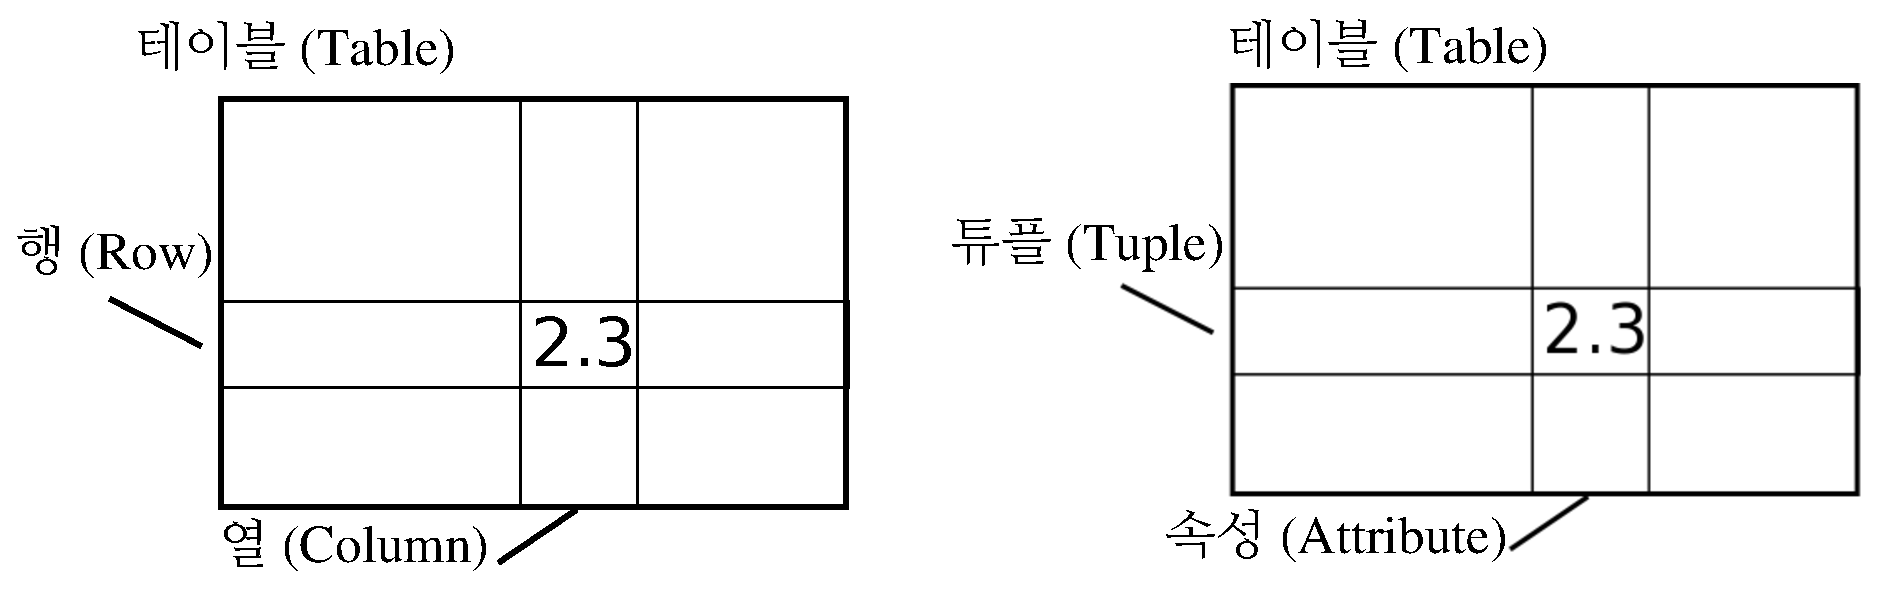
\includegraphics[height=1.50in]{figs2/relational.eps}}
\afterfig

관계형 데이터베이스의 기술적은 설명으로 테이블, 행, 열의 개념은 {\bf 관계(relation)}, {\bf 튜플(tuple)}, and {\bf 속성(attribute)} 각각 형식적으로 참조된다.
이번장에서는 좀더 덜 형식 용어를 사용한다.

\section{파이어폭스 애드온 SQLite 매니저}
SQLite 데이터베이스 파일에 데이터를 다루기 위해서 이번장에서 파이썬의 사용에 집중을 하지만, 다음 웹사이트에서 무료로 이용가능한
{\bf SQLite 데이터베이스 매니저(SQLite Database Manager)}로 불리는 파이어폭스 애드온을 사용해서 좀더 쉽게 많은 연산을 수행한다.

\url{https://addons.mozilla.org/en-us/firefox/addon/sqlite-manager/}

브라우져를 사용해서 쉽게 테이블을 생성하고, 데이터를 삽입, 편집하고 데이터베이스의 데이터에 간단한 SQL 질의를 실행할 수 있다.

이러한 점에서 데이터베이스 매니저는 텍스트 파일을 작업할 때 사용하는 텍스트 편집기와 유사하다.
텍스트 파일에 하나 혹은 몇개의 작업을 하고자 하면, 텍스트 편집기에 파일을 열어 원하는 수정을 하면 된다.
텍스트 파일에 작업할 사항이 많은 경우는 종종 간단한 파이썬 프로그램을 작성한다. 
데이터베이트로 작업할 때 동일한 패턴을 찾을 수 있다. 간단한 작업은 데이터베이스 매니저를 통해서 수행하고,
좀더 복잡한 작업은 파이썬으로 수행하는 것이 가장 편리하다.


\section{데이터베이스 테이블 생성하기}

데이터베이스는 파이썬 리스트 혹은 딕셔너리보다 좀더 명확히 정의된 구조를 요구한다.\footnote{
SQLite 실질적으로 열에 저장되는 데이터 형식에 좀더 많은 유연성을 부여하지만,
이번 장에서는 데이터 형식을 엄격하게 유지해서 MySQL 같은 다른 데이터베이스 시스템에도 동일하게 개념이 적용되게 한다.}.  

데이터베이스 {\bf 테이블(table)}을 생성할 때, 데이터베이스에게 테이블의 각 {\bf 열(column)}의 명칭과 각 {\bf 열(column)}에
저장하려고 하는 테이터의 형식을 미리 알려줘야 한다.
데이터베이스 소프트웨어가 각 열의 데이터 형식을 인식하게 되면, 데이터 형식에 따라 가장 효율적으로 데이터를 저장하고 찾아오는 방법을 선택할 수 있다.

다음 url에서 SQLite에서 지원하는 다양한 데이터 형식을 볼 수 있다.

\url{http://www.sqlite.org/datatypes.html}

처음에는 사전에 데이터 구조를 정의하는 것이 불편하게 보이지만, 데이터베이스가 대량의 데이터를 포함하는 경우에도 데이터의 빠른 접근을 보장하는 잇점이 있다.

데이터베이스 파일과 데이터베이스에 두개의 열을 가진 {\tt Tracks} 이름의 테이블을 생성하는 코드는 다음과 같다.

\index{sqlite3 module}
\index{module!sqlite3}
\beforeverb
\begin{verbatim}
import sqlite3

conn = sqlite3.connect('music.sqlite3')
cur = conn.cursor()

cur.execute('DROP TABLE IF EXISTS Tracks ')
cur.execute('CREATE TABLE Tracks (title TEXT, plays INTEGER)')

conn.close()
\end{verbatim}
\afterverb
%

\index{connect function}
\index{function!connect}
\index{cursor function}
\index{function!cursor}

{\tt connect} 연산은 현재 디렉토리의 {\tt music.sqlite3} 파일에 저장된 데이터베이스에 ''연결(connection)''한다.
파일이 존재하지 않으면, 자동 생성이 된다. ''연결(connection)''이라고 부르는 이유는 때때로 데이터베이스가 응용프로그램이 실행되는 서버로부터
분리된 ''데이터베이스 서버(database server)''에 저장되기 때문이다.
여기 간단한 예제에서는 데이터베이스가 실행되는 파이썬 코드처럼 동일한 디렉토리에 로컬 파일이다.

{\bf 커서(cursor)}는 파일을 다루는 파일핸들러처럼 데이터베이스에 저장된 파일에 연산을 수행하기 위해서 사용한다.
{\tt cursor()}를 호출하는 것은 개념적으로 텍스트 파일을 다룰 때 {\tt open()}을 호출하는 것과 개념적으로 매우 유사하다.

\beforefig
\centerline{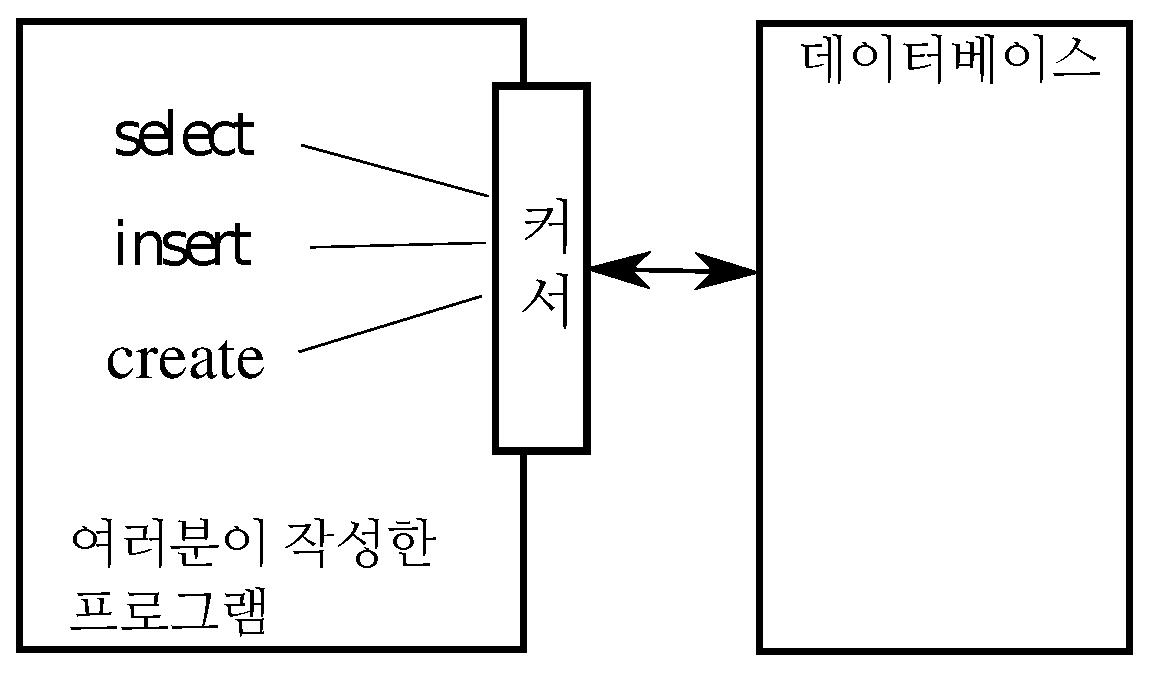
\includegraphics[height=1.50in]{figs2/cursor.eps}}
\afterfig

커서가 생성되면, {\tt execute()} 메쏘드를 사용하여 데이터베이스 콘텐츠에 명령어 실행을 할 수 있다.

데이터베이스 명령어는 특별한 언어로 표현되어 단 하나의 데이터베이스 언어를 학습하도록 서로 다른 많은 데이터베이스 업체사이에서 표준화되었다.
데이터베이스 언어는 {\bf SQL(Structured Query Language 구조적 질의 언어)}로 불린다.

\url{http://en.wikipedia.org/wiki/SQL}

상기 예제에서, 데이터베이스에 두개의 SQL 명령어를 실행했다. 관습적으로 데이터베이스 키워드는 대문자로 테이블이나 열의 명칭처럼 사용자가 추가한
명령어 부분은 소문자로 표기한다.

첫 SQL 명령어는 만약 존재한다면 데이터베이스에서 {\tt Tracks} 테이블을 삭제한다.
이런 형태의 패턴은 단순하게 오류 없이 반복적으로 {\tt Tracks} 테이블을 생성하도록 동일한 프로그램을 실행할 수 있게 한다.
{\tt DROP TABLE} 명령어는 데이터베이스로부터 테이블 및 테이블 콘텐츠 전부를 삭제함을 주목하세요. (즉, ''실행취소(undo)''가 없다.)

\beforeverb
\begin{verbatim}
cur.execute('DROP TABLE IF EXISTS Tracks ')
\end{verbatim}
\afterverb
%

두번째 명령어는 {\tt title} 문자형 열과 {\tt plays} 정수형 열을 가진 {\tt Tracks}으로 명명된 테이블을 생성한다.

\beforeverb
\begin{verbatim}
cur.execute('CREATE TABLE Tracks (title TEXT, plays INTEGER)')
\end{verbatim}
\afterverb
%

이제 {\tt Tracks}로 명명된 테이블을 생성했으니, SQL {\tt INSERT} 연산을 통해서 테이블에 데이터를 넣을 수 있다.
다시 한번, 데이터베이스에 연결하여 {\tt 커서(cursor)}를 얻어서 작업을 시작한다. 그리고 나서 커서를 사용하여 SQL 명령어를 수행한다.

SQL {\tt INSERT} 명령어는 어느 테이블을 사용하는지, {\tt (title, plays) }을 포함하는 필드를 통해서 신규 행을 정의하고 
테이블의 신규 행에 {\tt VALUES}에 해당 데이터를 입력한다.
실제 값이 {\tt execute()} 호출의 두번째 매개변수로 {\tt ( 'My Way', 15 ) } 튜플로 넘겨는 것을 표기하기 위해서 값을 물음표 {\tt (?, ?)}로 명기한다.

\beforeverb
\begin{verbatim}
import sqlite3

conn = sqlite3.connect('music.sqlite3')
cur = conn.cursor()

cur.execute('INSERT INTO Tracks (title, plays) VALUES ( ?, ? )', 
    ( 'Thunderstruck', 20 ) )
cur.execute('INSERT INTO Tracks (title, plays) VALUES ( ?, ? )', 
    ( 'My Way', 15 ) )
conn.commit()

print 'Tracks:'
cur.execute('SELECT title, plays FROM Tracks')
for row in cur :
   print row

cur.execute('DELETE FROM Tracks WHERE plays < 100')
conn.commit()

cur.close()
\end{verbatim}
\afterverb
%

먼저 테이블에 두개의 열을 {\tt 삽입(INSERT)}하고 {\tt commit()}을 사용하여 데이터가 데이터베이스에 써지도록 했다.

\beforefig
\centerline{\includegraphics[height=1.00in]{figs2/tracks.eps}}
\afterfig

그리고 나서, {\tt SELECT} 명령어를 사용하여 테이블에 방금전에 삽입된 행을 불러왔다.
{\tt SELECT} 명령어에 어느 열{\tt (title, plays)}을 가져오는지와 어느 테이블{\tt Tracks}에서 데이터를 가져올지를 나타낸다.
{\tt SELECT} 명령문을 수행한 후에, 커서는 {\tt for}문의 반복을 수행하는 것과 같다.
효율성을 위해서, 커서는 {\tt SELECT} 명령문을 수행할 때 데이터베이스에서 모든 데이터를 읽지 않는다. 
대신에 데이터는 {\tt for}문의 행을 반복하듯이 요청시에만 읽어온다.

프로그램 실행결과는 다음과 같다.

\beforeverb
\begin{verbatim}
Tracks:
(u'Thunderstruck', 20)
(u'My Way', 15)
\end{verbatim}
\afterverb
%
\index{Unicode}

{\tt for} 루프는 두개의 행을 읽어왔다. 각각의 행은 {\tt title}로 첫번째 값을,
{\tt plays}로 두번째 값을 가진 파이썬 튜플이다. title 문자열이 'u'로 시작한다고 걱정하지 마라.
해당 문자열은 라틴 문자가 아닌 다국어를 저장할 수 있는 {\bf 유니코드(Unicode)} 문자열을 나타내는 것이다.

프로그램 마지막에 SQL 명령어를 실행서 방금전에 생성한 행을 모두 {\tt 삭제(DELETE)}했서
프로그램을 다시금 실행할 수 있다. {\tt 삭제(DELETE)} 명령어는 {\tt WHERE} 문을 사용하여 선택 조건을 표기할 수 있다.
따라서 명령문이 조건을 충족하는 행에만 데이터베이스에 적용된다.
이번 예제에서 기준이 모든 행에 적용되어서 테이블에 아무 것도 없게 되어서 프로그램을 반복적으로 실행할 수 있다.
{\tt 삭제(DELETE)}를 실행한 후에 {\tt commit()}을 호출하여 데이터가 데이터베이스에서 와전히 제거되게 했다.

\section{SQL(Structured Query Language) 요약}

지금까지, 파이썬 예제에서 SQL(Structured Query Language)을 사용했고, SQL 명령어의 기본에 대해서 다루었다.
이번 장에서는 SQL 언어를 보고 SQL 구문 개요를 살펴본다.

대단히 많은 데이터베이스 업체가 존재하기 때문에 SQL(Structured Query Language)은 표준화가 많이 진행되었고,
여러 업체로부터 데이터베이스 시스템에 이식가능한 방식으로 의사소통이 가능하다.

관계형 데이터베이스는 테이블, 행과 열로 구성되어 있다. 행은 일반적으로 텍스트, 숫자, 혹은 날짜 형식의 데이터 형식이다.
테이블을 생성할 때, 열의 명칭과 형식을 지정한다.

\beforeverb
\begin{verbatim}
CREATE TABLE Tracks (title TEXT, plays INTEGER)
\end{verbatim}
\afterverb
%

테이블에 행을 삽입하기 위해서 SQL {\tt INSERT} 명령어를 사용한다.

\beforeverb
\begin{verbatim}
INSERT INTO Tracks (title, plays) VALUES ('My Way', 15)
\end{verbatim}
\afterverb
%

{\tt INSERT} 명령문은 테이블 이름을 명기하고 나서 새로운 행에 넣고 싶은 필드/행 리스트를 명시한다.
그리고 나서 키워드 {\tt VALUES}와 각 필드에 해당 값을 넣는다.

SQL {\tt SELECT} 명령어는 데이터베이스에서 행과 열을 가져오기 위해 사용된다.
{\tt SELECT} 명령문은 가져오고자 하는 행과 {\tt WHERE}절을 사용하여 어느 행을 가져올지를 지정한다.
선택사항으로 {\tt ORDER BY} 절을 이용하여 반환되는 행을 정렬할 수도 있다.

\beforeverb
\begin{verbatim}
SELECT * FROM Tracks WHERE title = 'My Way'
\end{verbatim}
\afterverb
%

\verb"*" 을 사용하여 {\tt WHERE} 절에 매칭되는 행의 모든 열을 데이터베이스에서 가져온다.

주목할 점은 파이썬과 달리 SQL {\tt WHERE} 절은 등식을 시험하기 위해서 두개의 등치 기호 보다 하나의 등치 기호를 사용한다.
{\tt WHERE}에서 인정되는 다른 논리 연산자는 
\verb"<",
\verb">",
\verb"<=",
\verb">=",
\verb"!=" 이고, 논리 표현식을 생성하는데 {\tt AND}와 {\tt OR}도 사용된다.

다음과 같이 반환되는 열이 필드값 중에 하나에 따라 정렬할 수도 있다.

\beforeverb
\begin{verbatim}
SELECT title,plays FROM Tracks ORDER BY title
\end{verbatim}
\afterverb
%

행을 제거하기 위해서, SQL {\tt DELETE} 명령문에 {\tt WHERE} 절이 필요하다.
{\tt WHERE} 절이 어느 행이 삭제될지 결정한다.

\beforeverb
\begin{verbatim}
DELETE FROM Tracks WHERE title = 'My Way'
\end{verbatim}
\afterverb
%

다음과 같이 SQL {\tt UPDATE} 명령문을 사용하여 테이블의 하나 혹은 그 이상의 행의 열을 {\tt 갱신(UPDATE)}한다.

\beforeverb
\begin{verbatim}
UPDATE Tracks SET plays = 16 WHERE title = 'My Way'
\end{verbatim}
\afterverb
%

{\tt UPDATE} 명령문은 테이블과 필드 리스트, 그리고 {\tt SET} 키워드 후에 바뀔 값을 명시한다.
그리고 선택사항으로 {\tt WHERE}절로 갱신될 열을 지정한다. 
단일 {\tt UPDATE} 명령문은 {\tt WHERE}절에 매칭되는 모든 행을 바꾼다. 만약 {\tt WHERE}절이 지정되지 않으면,
테이블의 모든 행에 대해서 {\tt 갱신(UPDATE)}을 한다.

4가지 기본 SQL 명령문(INSERT, SELECT, UPDATE, and DELETE)은 데이터를 생성하고 유지관리하는데 필요한 기본적인 4가지 작업을 가능케 한다.

\section{데이터베이스를 사용한 트위터 스파이더링(Spidering)}

이번장에서 트위커 계정을 통하고 계정 데이터베이스를 생성하는 간단한 스파이더링 프로그램을 작성합니다.
\emph{주의: 프로그램을 실행할 때 매우 주의하세요. 여러분의 트위터 계정의 접속이 차단될 정도로 너무 많은 데이터를 가져오거나 
장 시간 프로그램을 실행하지 마세요.}

임의의 스파이더링 프로그램이 가지는 문제점 중의 하나는 중단되거나 여러번 재시작할 필요가 생겨서
지금까지 가져온 데이터를 여러분은 잃고 싶지 않습니다.
처음에 데이터 가져오기를 항상 다시 시작하고 싶지 않고,
데이터를 가져오면 저장하길 원한다.
그래서 프로그램이 저장을 시작할 수 있고, 중단한 곳에서 다시 가져오길 원합니다.

한 사람의 트위터 친구와 상태 정보를 가져오는 것에서, 친구의 리스트에서 반복적으로 적용하고, 친구 각각을 향후에 가져올 수 있도록 데이터베이스에 추가하여 시작한다. 
한 사람의 트위터 친구를 처리한 후에 테이터베이스를 확인하고 친구의 친구 한명을 가져온다. 이것을 반복하고, ''방문하지 않는(unvisited)'' 친구를 선택하고,
친구의 리스트를 가져오고 향후 방문을 위해서 리스트에 보지 않은 친구로 추가한다.

''인기도(popularity)''를 측정하도록 데이터베이스에 특별한 친구를 얼마나 자주 봤는지를 기록한다.

알고 있는 계정 리스트르 저장함으로써, 혹은 계정을 가져왔는 혹은 그렇지 않은지, 그리고 계정이 컴퓨터 디스크의 데이터베이스에서 얼마나 인기있는지에 따라
원하는 만큼 프로그램을 멈추거나 다시 시작할 수 있다.

% TODO: Add a reference to the right spot
프로그램이 약간 복잡하다. 트위터 API를 사용한 책의 앞뽁 예제에서 가져온 코드에 기반한다.

다음은 트위터 스파이더링 응용프로그램의 소스코드다.

\beforeverb
\begin{verbatim}
import urllib
import twurl
import json
import sqlite3

TWITTER_URL = 'https://api.twitter.com/1.1/friends/list.json'

conn = sqlite3.connect('spider.sqlite3')
cur = conn.cursor()

cur.execute('''
CREATE TABLE IF NOT EXISTS Twitter 
(name TEXT, retrieved INTEGER, friends INTEGER)''')

while True:
    acct = raw_input('Enter a Twitter account, or quit: ')
    if ( acct == 'quit' ) : break
    if ( len(acct) < 1 ) :
        cur.execute('SELECT name FROM Twitter WHERE retrieved = 0 LIMIT 1')
        try:
            acct = cur.fetchone()[0]
        except:
            print 'No unretrieved Twitter accounts found'
            continue

    url = twurl.augment(TWITTER_URL, 
               {'screen_name': acct, 'count': '20'} )
    print 'Retrieving', url
    connection = urllib.urlopen(url)
    data = connection.read()
    headers = connection.info().dict
    # print 'Remaining', headers['x-rate-limit-remaining']
    js = json.loads(data)
    # print json.dumps(js, indent=4)

    cur.execute('UPDATE Twitter SET retrieved=1 WHERE name = ?', (acct, ) )

    countnew = 0
    countold = 0
    for u in js['users'] :
        friend = u['screen_name']
        print friend
        cur.execute('SELECT friends FROM Twitter WHERE name = ? LIMIT 1', 
            (friend, ) )
        try:
            count = cur.fetchone()[0]
            cur.execute('UPDATE Twitter SET friends = ? WHERE name = ?', 
                (count+1, friend) )
            countold = countold + 1
        except:
            cur.execute('''INSERT INTO Twitter (name, retrieved, friends) 
                VALUES ( ?, 0, 1 )''', ( friend, ) )
            countnew = countnew + 1
    print 'New accounts=',countnew,' revisited=',countold
    conn.commit()

cur.close()
\end{verbatim}
\afterverb
%



Our database is stored in the file {\tt spider.sqlite3} and it has one 
table named {\tt Twitter} and each row in the {\tt Twitter} table
has a column for the account name, whether we have retrieved the friends
of this account, and how many times this account has been ``friended''.

In the main loop of the program, we prompt the user for a Twitter
account name or ``quit'' to exit the program.  
If the user enters a Twitter account, we retrieve the 
list of friends and statuses
for that user and add each friend to the database if 
not already in the database.  If the friend is already in the list, 
we add one to the {\tt friends} field in the row in the database.

If the user presses enter, we look in the database for the next 
Twitter account that we have not yet retrieved and retrieve the
friends and statuses for that account, add them to the database 
or update them and increase their {\tt friends count}.

Once we retrieve the list of friends and statuses, we loop 
through all of the {\tt user} items in the returned JSON
and retrieve the \verb"screen_name" for each user.  Then we use
the {\tt SELECT } statement to see if we already have stored this
particular \verb"screen_name" in the database and retrieve the
friend count ({\tt friends}) if the record exists.

\beforeverb
\begin{verbatim}
    countnew = 0
    countold = 0
    for u in js['users'] :
        friend = u['screen_name']
        print friend
        cur.execute('SELECT friends FROM Twitter WHERE name = ? LIMIT 1', 
            (friend, ) )
        try:
            count = cur.fetchone()[0]
            cur.execute('UPDATE Twitter SET friends = ? WHERE name = ?', 
                (count+1, friend) )
            countold = countold + 1
        except:
            cur.execute('''INSERT INTO Twitter (name, retrieved, friends) 
                VALUES ( ?, 0, 1 )''', ( friend, ) )
            countnew = countnew + 1
    print 'New accounts=',countnew,' revisited=',countold
    conn.commit()
\end{verbatim}
\afterverb
%
Once the cursor executes the {\tt SELECT} statement, 
we must retrieve the rows.  We could do this with a {\tt for} 
statement, but since we are only retrieving
one row ({\tt LIMIT 1}), we can use the {\tt fetchone()} method to fetch the
first (and only) row that is the result of the {\tt SELECT} operation.  
Since {\tt fetchone()} returns the row as a {\bf tuple} (even though there is only
one field), we take the first value from the tuple using {\tt [0]} to get the 
current friend count into the variable {\tt count}.  

If this retrieval is successful, we use the SQL {\tt UPDATE} statement with a 
{\tt WHERE} clause to add one to the {\tt friends} column for the row that 
matches the friend's account.  Notice that there are two placeholders (i.e.
question marks) in the SQL, and the second parameter to the {\tt execute()} is
a two-element tuple which holds the values to be substituted into the SQL
in place of the question marks.

If the code in the {\tt try} block fails it is probably because no record
matched the {\tt WHERE name = ?} clause on the SELECT statement.  So in the
{\tt except} block, we use the SQL {\tt INSERT} statement to add the friend's
\verb"screen_name" to the table with an indication that we have not yet 
retrieved the \verb"screen_name" and setting the friend count to zero.

So the first time the program runs and we enter a Twitter account, the program
runs as follows:

\beforeverb
\begin{verbatim}
Enter a Twitter account, or quit: drchuck
Retrieving http://api.twitter.com/1.1/friends ...
New accounts= 20  revisited= 0
Enter a Twitter account, or quit: quit
\end{verbatim}
\afterverb
%
Since this is the first time we have run the program, the database
is empty and we create the database in the file {\tt spider.sqlite3} and
add a table named {\tt Twitter} to the database.  Then we retrieve
some friends and add them all to the database since the database is
empty.

At this point, we might want to write a simple database dumper
to take a look at what is in our {\tt spider.sqlite3} file:

\beforeverb
\begin{verbatim}
import sqlite3

conn = sqlite3.connect('spider.sqlite3')
cur = conn.cursor()
cur.execute('SELECT * FROM Twitter')
count = 0
for row in cur :
   print row
   count = count + 1
print count, 'rows.'
cur.close()
\end{verbatim}
\afterverb
%
This program simply opens the database and selects all of the 
columns of all of the rows in the table {\tt Twitter}, then 
loops through the rows and prints out each row.

If we run this program after the first execution of our Twitter
spider above, its output will be as follows:

\beforeverb
\begin{verbatim}
(u'opencontent', 0, 1)
(u'lhawthorn', 0, 1)
(u'steve_coppin', 0, 1)
(u'davidkocher', 0, 1)
(u'hrheingold', 0, 1)
...
20 rows.
\end{verbatim}
\afterverb
%
We see one row for each \verb"screen_name", that we 
have not retrieved the data for that \verb"screen_name" and 
everyone in the database has one friend.

Now our database reflects the retrieval of the friends of 
our first Twitter account ({\bf drchuck}).  We can run the program
again and tell it to retrieve the friends of the next 
``unprocessed'' account by simply pressing enter instead of
a Twitter account as follows:

\beforeverb
\begin{verbatim}
Enter a Twitter account, or quit: 
Retrieving http://api.twitter.com/1.1/friends ...
New accounts= 18  revisited= 2
Enter a Twitter account, or quit: 
Retrieving http://api.twitter.com/1.1/friends ...
New accounts= 17  revisited= 3
Enter a Twitter account, or quit: quit
\end{verbatim}
\afterverb
%
Since we pressed enter (i.e. we did not specify a Twitter account),
the following code is executed:

\beforeverb
\begin{verbatim}
    if ( len(acct) < 1 ) :
        cur.execute('SELECT name FROM Twitter WHERE retrieved = 0 LIMIT 1')
        try:
            acct = cur.fetchone()[0]
        except:
            print 'No unretrieved twitter accounts found'
            continue
\end{verbatim}
\afterverb
%
We use the SQL {\tt SELECT} statement to retrieve the name of the first 
({\tt LIMIT 1}) user who still has their ``have we retrieved this user''
value set to zero.  We also use the {\tt fetchone()[0]} pattern within 
a try/except block to either extract a \verb"screen_name" from the retrieved
data or put out an error message and loop back up.

If we successfully retrieved an unprocessed \verb"screen_name", we retrieve
their data as follows:

\beforeverb
\begin{verbatim}
    url = twurl.augment(TWITTER_URL, {'screen_name': acct, 'count': '20'} )
    print 'Retrieving', url
    connection = urllib.urlopen(url)
    data = connection.read()
    js = json.loads(data)

    cur.execute('UPDATE Twitter SET retrieved=1 WHERE name = ?', (acct, ) )
\end{verbatim}
\afterverb
%
Once we retrieve the data successfully, we use the {\tt UPDATE} statement 
to set the {\tt retrieved} column to one to indicate that we have completed 
the retrieval of the friends of this account.  This keeps us from re-retrieving
the same data over and over and keeps us progressing forward through the network
of Twitter friends.

If we run the friend program and press enter twice to retrieve the next 
unvisited friend's friends,
then run the dumping program, it will give us the following output:

\beforeverb
\begin{verbatim}
(u'opencontent', 1, 1)
(u'lhawthorn', 1, 1)
(u'steve_coppin', 0, 1)
(u'davidkocher', 0, 1)
(u'hrheingold', 0, 1)
...
(u'cnxorg', 0, 2)
(u'knoop', 0, 1)
(u'kthanos', 0, 2)
(u'LectureTools', 0, 1)
...
55 rows.
\end{verbatim}
\afterverb
%
We can see that we have properly recorded that we have visited 
{\tt lhawthorn} and {\tt opencontent}.  Also the accounts 
{\tt cnxorg} and {\tt kthanos} already have two followers.
Since we now have retrieved the friends of three people
({\tt drchuck}, {\tt opencontent} and {\tt lhawthorn}) our table has 55 rows 
of friends to retrieve.

Each time we run the program and press enter, it will pick the next 
unvisited account (e.g. the next account will be \verb"steve_coppin"),
retrieve their friends, mark them as retrieved and for each of the 
friends of \verb"steve_coppin", either add them to the end of the 
database, or update their friend count if they are already in the
database.

Since the program's data is all stored on disk in a database, 
the spidering activity can be suspended and resumed as many times as you 
like with no loss of data.

\section{데이터 모델링 기초}

관계형 데이터베이스의 진정한 힘은 다중 테이블과 테이블 사이의 관계를 생성할 때다.
응용프로그램의 데이터를 쪼개서 다중 테이블과 두 테이블 사이의 관계를 설정하는 결정을 
{\bf 데이터 모델링(data modeling)}이라고 한다. 테이블과 테이블 관계를 보여주는 설계 문서를 
{\bf 데이터 모델(data model)}이라고 한다.

데이터 모델링은 상대적으로 고급 기술이여서 이번 장에서는 관계형 데이터 모델링의 가장 기본적인 개념만을 소개한다.
좀더 데이터 모델링의 자세한 사항은 아래 링크에서 시작해볼 수 있다.

\url{http://en.wikipedia.org/wiki/Relational_model}

한 사람의 친구를 단순히 몇명인지 세는 대신에 트위터 스파이더 응용프로그램으로 모든 관계 리스트를 가지고서 특정한 계정에
팔로잉하는 모든 사람을 찾을 수 있다.

모든 사람은 팔로잉하는 계정을 많이 가지고 있어서, {\tt 트위터(Twitter)} 테이블에 단순히 하나의 열만을 추가할 수는 없다.
그래서 친구를 짝으로 추적할 수 있는 새로운 테이블을 생성한다. 다음은 그런 테이블을 생성하는 간단한 방식이다.

\beforeverb
\begin{verbatim}
CREATE TABLE Pals (from_friend TEXT, to_friend TEXT)
\end{verbatim}
\afterverb
%

{\tt drchuck}을 팔로잉하는 사람을 마주칠 때마다, 다음 형식의 행을 삽입한다.

\beforeverb
\begin{verbatim}
INSERT INTO Pals (from_friend,to_friend) VALUES ('drchuck', 'lhawthorn')
\end{verbatim}
\afterverb
%

{\tt drchuck} 트위터 피드에서 20명의 친구를 처리하면서, ''drchuck''을 첫 매개변수로 가지는 20개 레코드를 삽입해서
데이터베이스에 많이 중복되는 문자열을 가질 것이다.

문자열 데이터를 중복하는 것은 {\bf 데이터베이스 정규화(database normalization)}의 가장 좋은 사례를 위반한다.
데이터베이스 정규화는 결코 한번 이상 데이터베이스에 동일한 문자열을 놓지 않는다. 
만약 한번 이상 데이터가 필요하다면, 데이터에 대한 숫자 {\bf 키(key)}를 생성하고, 키를 사용하여 실제 데이터를 참조한다.

실무에서, 문자열은 컴퓨터상의 주기억장치나 디스크상의 정수형 자료보다 훨씬 많은 공간을 차지하고 비교나 정렬에 더 많은 처리시간이 소요된다.
수백개의 항목이 있다면, 저장소나 처리 시간은 큰 문제가 되지 않는다. 하지만, 데이터베이스에 수백만명의 사람 정보와 1억건 이상의 링크가 있다면,
가능한 빨리 데이터를 스캔하는 것이 중요하다.

앞선 예제에서 사용된 {\tt Twitter} 테이블 대신에 {\tt People}로 명명된 테이블에 트위커 계정을 저장한다.
{\tt People} 테이블은 트위터 사용자의 행과 관련된 숫자키를 저장할 수 있는 추가 열(column)이 있다.
SQLite는 데이터 열의 특별 형식({\tt INTEGER PRIMARY KEY})을 이용하여 테이블에 삽입할 임의의 열에 대해서 자동적으로 키값을 추가하는 기능이 있다.

다음과 같이 추가적인 {\tt id} 열을 가진 {\tt People} 테이블을 생성할 수 있다.

\beforeverb
\begin{verbatim}
CREATE TABLE People 
    (id INTEGER PRIMARY KEY, name TEXT UNIQUE, retrieved INTEGER)
\end{verbatim}
\afterverb
%

{\tt People} 테이블의 각 행에서 친구 숫자를 더 이상 유지하고 있지 않음을 주목하세요.
{\tt id} 열의 형식으로 {\tt INTEGER PRIMARY KEY} 선택할 때, SQLite가 이 행을 맡아서 
사용자가 삽입하는 각 항에 자동으로 유일한 숫자 키를 할당하도록 나타낸다.
{\tt UNIQUE} 키워드를 추가해서 {\tt name}에 동일한 값을 가진 두 행이 SQLite가 삽입하지 못하도록 나타낸다.

위에 {\tt Pals} 테이블을 생성하는 대신에 데이터베이스에 \verb"from_id", \verb"to_id" 두 정수 열을 지니고 
\verb"from_id"과 \verb"to_id"의 \emph{조합}은 테이블에 유일하다는 제약사항을 가진 {\tt Follows} 테이블을 생성한다.(즉, 중복된 행을 삽입할 수 없다.)

\beforeverb
\begin{verbatim}
CREATE TABLE Follows 
    (from_id INTEGER, to_id INTEGER, UNIQUE(from_id, to_id) )
\end{verbatim}
\afterverb
%

테이블에 {\tt UNIQUE}절을 추가할 때, 레코드를 삽입할 때 데이터베이스에서 지켜야하는 규칙의 집합을 의사소통하는 것이다.
잠시 후에 보겠지만, 프로그램상에 편리하게 이러한 규칙을 생성한다.
이 규칙은 실수를 방지하게 하고 코드를 작성을 간결하게 한다.

본질적으로 {\tt Follows} 테이블을 생성할 때, ''관계(relationship)''를 모델링하여 한 사람이 다른 사람을 ''팔로우(follow)''하고
이것을 (a) 사람이 연결되어 있고, (b) 관계을 방향성이 나타나도록 숫자 짝을 지어 표현한다.  

\beforefig
\centerline{\includegraphics[height=2.50in]{figs2/twitter.eps}}
\afterfig

\section{Programming with multiple tables}

We will now re-do the Twitter spider program using two tables, the primary
keys, and the key references as described above.  Here is the code for 
the new version of the program:

\beforeverb
\begin{verbatim}
import urllib
import twurl
import json
import sqlite3

TWITTER_URL = 'https://api.twitter.com/1.1/friends/list.json'

conn = sqlite3.connect('friends.sqlitesqlite3')
cur = conn.cursor()

cur.execute('''CREATE TABLE IF NOT EXISTS People 
    (id INTEGER PRIMARY KEY, name TEXT UNIQUE, retrieved INTEGER)''')
cur.execute('''CREATE TABLE IF NOT EXISTS Follows 
    (from_id INTEGER, to_id INTEGER, UNIQUE(from_id, to_id))''')

while True:
    acct = raw_input('Enter a Twitter account, or quit: ')
    if ( acct == 'quit' ) : break
    if ( len(acct) < 1 ) :
        cur.execute('''SELECT id, name FROM People 
            WHERE retrieved = 0 LIMIT 1''')
        try:
            (id, acct) = cur.fetchone()
        except:
            print 'No unretrieved Twitter accounts found'
            continue
    else:
        cur.execute('SELECT id FROM People WHERE name = ? LIMIT 1', 
            (acct, ) )
        try:
            id = cur.fetchone()[0]
        except:
            cur.execute('''INSERT OR IGNORE INTO People (name, retrieved) 
                VALUES ( ?, 0)''', ( acct, ) )
            conn.commit()
            if cur.rowcount != 1 : 
                print 'Error inserting account:',acct
                continue
            id = cur.lastrowid

    url = twurl.augment(TWITTER_URL, 
       {'screen_name': acct, 'count': '20'} )
    print 'Retrieving account', acct
    connection = urllib.urlopen(url)
    data = connection.read()
    headers = connection.info().dict
    print 'Remaining', headers['x-rate-limit-remaining']

    js = json.loads(data)
    # print json.dumps(js, indent=4)

    cur.execute('UPDATE People SET retrieved=1 WHERE name = ?', (acct, ) )

    countnew = 0
    countold = 0
    for u in js['users'] :
        friend = u['screen_name']
        print friend
        cur.execute('SELECT id FROM People WHERE name = ? LIMIT 1', 
            (friend, ) )
        try:
            friend_id = cur.fetchone()[0]
            countold = countold + 1
        except:
            cur.execute('''INSERT OR IGNORE INTO People (name, retrieved) 
                VALUES ( ?, 0)''', ( friend, ) )
            conn.commit()
            if cur.rowcount != 1 :
                print 'Error inserting account:',friend
                continue
            friend_id = cur.lastrowid
            countnew = countnew + 1
        cur.execute('''INSERT OR IGNORE INTO Follows (from_id, to_id) 
            VALUES (?, ?)''', (id, friend_id) )
    print 'New accounts=',countnew,' revisited=',countold
    conn.commit()

cur.close()
\end{verbatim}
\afterverb
%
This program is starting to get a bit complicated, but it illustrates
the patterns that we need to use when we are
using integer keys to link tables. The basic patterns are:

\begin{enumerate}

\item Creating tables with primary keys and constraints.

\item When we have a logical key for a person (i.e. account
name) and we need the {\tt id} value for the person.
Depending on whether or not the person is already
in the {\tt People} table, we either need to: 
(1) look up the person in the {\tt People} table and 
retrieve the {\tt id} value for the person 
or (2) add the person to the {\tt People} table and get the 
{\tt id} value for the newly added row.

\item Insert the row that captures the ``follows'' relationship.

\end{enumerate}

We will cover each of these in turn.

\subsection{Constraints in database tables}

As we design our table structures, we can tell the database system 
that we would like it to enforce a few rules on us.   These rules
help us from making mistakes and introducing incorrect data into 
out tables.   When we create our tables:

\beforeverb
\begin{verbatim}
cur.execute('''CREATE TABLE IF NOT EXISTS People 
    (id INTEGER PRIMARY KEY, name TEXT UNIQUE, retrieved INTEGER)''')
cur.execute('''CREATE TABLE IF NOT EXISTS Follows 
    (from_id INTEGER, to_id INTEGER, UNIQUE(from_id, to_id))''')
\end{verbatim}
\afterverb
%
We indicate that the {\tt name} column in the {\tt People} table must be
{\tt UNIQUE}.   We also indicate that the combination of the two numbers
in each row of the {\tt Follows} table must be unique.  These constraints
keep us from making mistakes such as adding the same relationship more than
once.

We can take advantage of these constraints in the following code:

\beforeverb
\begin{verbatim}
cur.execute('''INSERT OR IGNORE INTO People (name, retrieved) 
    VALUES ( ?, 0)''', ( friend, ) )
\end{verbatim}
\afterverb
%
We add the {\tt OR IGNORE} clause to our {\tt INSERT} statement to indicate
that if this particular {\tt INSERT} would cause a violation of the
``{\tt name} must be unique'' rule, the database system is allowed to ignore the 
{\tt INSERT}.  We are using the database constraint as a safety net
to make sure we don't inadvertently do something incorrect.

Similarly, the following code ensures that we don't add the 
exact same {\tt Follows} relationship twice.

\beforeverb
\begin{verbatim}
cur.execute('''INSERT OR IGNORE INTO Follows 
    (from_id, to_id) VALUES (?, ?)''', (id, friend_id) )
\end{verbatim}
\afterverb
%
Again we simply tell the database to ignore our attempted 
{\tt INSERT} if it would violate the uniqueness constraint
that we specified for the {\tt Follows} rows.

\subsection{Retrieve and/or insert a record}

When we prompt the user for a Twitter account, if the account 
exists, we must look up its {\tt id} value.  If the account
does not yet exist in the {\tt People} table, we must insert 
the record and get the {\tt id} value from the inserted
row.

This is a very common pattern and is done twice in the program above.
This code shows how we look up the {\tt id} for a 
friend's account when we have extracted a \verb"screen_name"
from a {\tt user} node in the retrieved Twitter JSON.

Since over time it will be increasingly likely that the account
will already be in the database, we first check to see if the
{\tt People} record exists using a {\tt SELECT} statement.

If all goes well\footnote{In general, when a sentence starts 
with ``if all goes well'' you will find that the code needs
to use try/except.} inside the {\tt try} section, we retrieve the
record using {\tt fetchone()} and then retrieve the
first (and only) element of the returned tuple and store it in 
\verb"friend_id".

If the {\tt SELECT} fails, the {\tt fetchone()[0]} code will fail
and control will transfer into the {\tt except} section.

\beforeverb
\begin{verbatim}
        friend = u['screen_name']
        cur.execute('SELECT id FROM People WHERE name = ? LIMIT 1',
            (friend, ) )
        try:
            friend_id = cur.fetchone()[0]
            countold = countold + 1
        except:
            cur.execute('''INSERT OR IGNORE INTO People (name, retrieved) 
                VALUES ( ?, 0)''', ( friend, ) )
            conn.commit()
            if cur.rowcount != 1 :
                print 'Error inserting account:',friend
                continue
            friend_id = cur.lastrowid
            countnew = countnew + 1
\end{verbatim}
\afterverb
%
If we end up in the {\tt except} code, it simply means that the row
was not found so we must insert the row.  We use {\tt INSERT OR 
IGNORE} just to avoid errors and then call {\tt commit()} to 
force the database to really be updated.  After the write is done, we can 
check the {\tt cur.rowcount} to see how many rows were affected.  Since
we are attempting to insert a single row, if the number of 
affected rows is something other than one, it is an error.  

If the {\tt INSERT} is successful, we can look at {\tt cur.lastrowid} 
to find out what value the database assigned to the {\tt id} column in 
our newly created row.

\subsection{Storing the friend relationship}

Once we know the key value for both the Twitter user
and the friend in the JSON, it is a simple matter to insert
the two numbers into the {\tt Follows} table
with the following code:

\beforeverb
\begin{verbatim}
cur.execute('INSERT OR IGNORE INTO Follows (from_id, to_id) VALUES (?, ?)',
    (id, friend_id) )
\end{verbatim}
\afterverb
%
Notice that we let the database take care of keeping us from ``double-inserting''
a relationship by creating the table with a uniqueness constraint and then
adding {\tt OR IGNORE} to our {\tt INSERT} statement.

Here is a sample execution of this program:

\beforeverb
\begin{verbatim}
Enter a Twitter account, or quit: 
No unretrieved Twitter accounts found
Enter a Twitter account, or quit: drchuck
Retrieving http://api.twitter.com/1.1/friends ...
New accounts= 20  revisited= 0
Enter a Twitter account, or quit: 
Retrieving http://api.twitter.com/1.1/friends ...
New accounts= 17  revisited= 3
Enter a Twitter account, or quit: 
Retrieving http://api.twitter.com/1.1/friends ...
New accounts= 17  revisited= 3
Enter a Twitter account, or quit: quit
\end{verbatim}
\afterverb
%
We started with the {\tt drchuck} account and then let the program
automatically pick the next two accounts to retrieve and add to 
our database.

The following is the first few rows in the {\tt People} 
and {\tt Follows} tables after this run is completed:

\beforeverb
\begin{verbatim}
People:
(1, u'drchuck', 1)
(2, u'opencontent', 1)
(3, u'lhawthorn', 1)
(4, u'steve_coppin', 0)
(5, u'davidkocher', 0)
55 rows.
Follows:
(1, 2)
(1, 3)
(1, 4)
(1, 5)
(1, 6)
60 rows.
\end{verbatim}
\afterverb
%
You can see the {\tt id}, {\tt name}, and {\tt visited} fields in the 
{\tt People} table and you see the numbers of both ends of 
the relationship {\tt Follows} table.   
In the {\tt People} table, we can see that the first three people
have been visited and their data has been retrieved.
The data in the {\tt Follows} table indicates that
{\tt drchuck} (user 1) is a friend to all of the people shown in the first
five rows.  This makes sense because
the first data we retrieved and stored was the Twitter friends of
{\tt drchuck}.  If you were to print more rows from the {\tt Follows} table,
you would see the friends of user two and three as well.

\section{Three kinds of keys}

Now that we have started building a data model putting our
data into multiple linked tables, and linking the rows in those
tables using {\bf keys}, we need to look at some terminology 
around keys.  There are generally three kinds of keys used 
in a database model.

\begin{itemize}

\item A {\bf logical key} is a key that the ``real world'' might use
to look up a row.   In our example data model, the {\tt name}
field is a logical key.  It is the screen name for the user 
and we indeed look up a user's row several times in the program
using the {\tt name} field.  You will often find that it makes
sense to add a {\tt UNIQUE} constraint to a logical key.  Since the 
logical key is how we look up a row from the outside world, it makes
little sense to allow multiple rows with the same value in the table.

\item A {\bf primary key} is usually a number that is assigned
automatically by the database.  It generally has no meaning outside
the program and is only used to link rows from different tables
together.  When we want to look up a row in a table, usually 
searching for the row using the primary key is the fastest 
way to find a row.  Since primary keys are integer numbers, they 
take up very little storage and can be compared or sorted very quickly.
In our data model, the {\tt id} field is an example of a primary key.

\item A {\bf foreign key} is usually a number that points to the primary key
of an associated row in a different table.  An example of a foreign
key in our data model is the \verb"from_id".  

\end{itemize}

We are using a
naming convention of always calling the primary key field name
{\tt id} and appending the suffix \verb"_id" to any field name
that is a foreign key.


\section{Using JOIN to retrieve data}

Now that we have followed the rules of database normalization
and have data separated into two tables, linked together using
primary and foreign keys, we need to be able to build a 
{\tt SELECT} that re-assembles the data across the tables.

SQL uses the {\tt JOIN} clause to re-connect these tables.  
In the {\tt JOIN} clause you specify the fields that are used 
to re-connect the rows between the tables.

The following is an example of a {\tt SELECT} with a 
{\tt JOIN} clause:

\beforeverb
\begin{verbatim}
SELECT * FROM Follows JOIN People 
    ON Follows.from_id = People.id WHERE People.id = 1
\end{verbatim}
\afterverb
%
The {\tt JOIN} clause indicates that the fields we are selecting
cross both the {\tt Follows} and {\tt People} tables.  The {\tt ON}
clause indicates how the two tables are to be joined.   Take the rows
from {\tt Follows} and append the row from {\tt People} where the
field \verb"from_id" in {\tt Follows} is the same the {\tt id} value
in the {\tt People} table.

\beforefig
\centerline{\includegraphics[height=2.50in]{figs2/join.eps}}
\afterfig

The result of the JOIN is to create extra-long ``meta-rows'' which have both 
the fields from {\tt People} and the matching fields from {\tt Follows}.
Where there is more than one match between the {\tt id} field from {\tt People}
and the \verb"from_id" from {\tt People}, then JOIN creates a meta-row 
for \emph{each} of the matching pairs of rows, duplicating data as needed.

The following code demonstrates the data that we will have in the 
database after the multi-table Twitter spider program (above) has
been run several times.

\beforeverb
\begin{verbatim}
import sqlite3

conn = sqlite3.connect('spider.sqlite3')
cur = conn.cursor()

cur.execute('SELECT * FROM People')
count = 0
print 'People:'
for row in cur :
   if count < 5: print row
   count = count + 1
print count, 'rows.'

cur.execute('SELECT * FROM Follows')
count = 0
print 'Follows:'
for row in cur :
   if count < 5: print row
   count = count + 1
print count, 'rows.'

cur.execute('''SELECT * FROM Follows JOIN People 
    ON Follows.from_id = People.id WHERE People.id = 2''')
count = 0
print 'Connections for id=2:'
for row in cur :
   if count < 5: print row
   count = count + 1
print count, 'rows.'

cur.close()
\end{verbatim}
\afterverb
%
In this program, we first dump out the {\tt People}
and {\tt Follows} and then dump out a subset of the
data in the tables joined together.

Here is the output of the program:

\beforeverb
\begin{verbatim}
python twjoin.py 
People:
(1, u'drchuck', 1)
(2, u'opencontent', 1)
(3, u'lhawthorn', 1)
(4, u'steve_coppin', 0)
(5, u'davidkocher', 0)
55 rows.
Follows:
(1, 2)
(1, 3)
(1, 4)
(1, 5)
(1, 6)
60 rows.
Connections for id=2:
(2, 1, 1, u'drchuck', 1)
(2, 28, 28, u'cnxorg', 0)
(2, 30, 30, u'kthanos', 0)
(2, 102, 102, u'SomethingGirl', 0)
(2, 103, 103, u'ja_Pac', 0)
20 rows.
\end{verbatim}
\afterverb
%
You see the columns from the {\tt People} and {\tt Follows} tables and the last
set of rows is the result of the {\tt SELECT} with the {\tt JOIN} clause.

In the last select, we are looking for accounts that are friends of 
``opencontent'' (i.e. {\tt People.id=2}).

In each of the ``meta-rows'' in the last select, the first two columns are
from the {\tt Follows}
table followed by columns three through five from the {\tt People} table.  You can also
see that the second column (\verb"Follows.to_id") matches the third column
({\tt People.id}) in each of the joined-up ``meta-rows''.

\section{Summary}

This chapter has covered a lot of ground to give you an overview of the basics
of using a database in Python.   It is more complicated to write the code to use 
a database to store data than Python dictionaries or flat files so there is 
little reason to use a database unless your application truly needs the capabilities
of a database.  The situations where a database can be quite useful are: 
(1) when your application needs to make small many random updates within a large data set,
(2) when your data is so large it cannot fit in a dictionary and you need to 
look up information repeatedly, or
(3) you have a long-running process that you want to be able to stop 
and restart and retain the data from one run to the next.

You can build a simple database with a single table to suit many application 
needs, but most problems will require several tables and links/relationships
between rows in different tables.   When you start making links between 
tables, it is important to do some thoughtful design and follow the 
rules of database normalization to make the best use of the database's
capabilities.  Since the primary motivation for using a database
is that you have a large amount of data to deal with, it is important
to model your data efficiently so your programs run as fast as possible.

\section{Debugging}

One common pattern when you are developing a Python program to connect to
an SQLite database will be to run a Python program and check the
results using the SQLite Database Browser.  The browser allows you 
to quickly check to see if your program is working properly.

You must be careful because SQLite takes care to keep two programs
from changing the same data at the same time.   For example, if
you open a database in the browser and make a change to the database
and have not yet pressed the ``save'' button in the browser, the 
browser ``locks'' the database file and keeping any other program
from accessing the file.  In particular, your Python program
will not be able to access the file if it is locked.

So a solution is to make sure to either close the database browser 
or use the {\bf File} menu to close the database in the browser
before you attempt to access the database from Python to avoid
the problem of your Python code failing because the database is
locked.

\section{Glossary}

\begin{description}

\item[attribute:] One of the values within a tuple.  More commonly
called a ``column'' or ``field''.
\index{attribute}

\item[constraint:] 
When we tell the database to enforce a rule on a field or a row
in a table.  A common constraint is to insist that there can be no
duplicate values in a particular field (i.e. all the values must be unique).
\index{constraint}

\item[cursor:] A cursor allows you to execute SQL commands in a database
and retrieve data from the database.  A cursor is similar to 
a socket or file handle for network connections and files respectively.
\index{cursor}

\item[database browser:] 
A piece of software that allows you to directly connect to a database 
and manipulate the database directly without writing a program.
\index{database browser}

\item[foreign key:] A numeric key that points to the primary key of 
a row in another table.  Foreign keys establish relationships between rows
stored in different tables.
\index{foreign key}

\item[index:] Additional data that the database software maintains as rows
are inserted into a table designed to make lookups very fast.
\index{index}

\item[logical key:] A key that the ``outside world'' uses to look up a particular
row.  For example in a table of user accounts, a person's e-mail address
might be a good candidate as the logical key for the user's data. 
\index{logical key}

\item[normalization:] Designing a data model so that no data
is replicated.  We store each item of data at one place in the database
and reference it elsewhere using a foreign key.
\index{normalization}
\index{database normalization}

\item[primary key:] A numeric key assigned to each row that is used to 
refer to one row in a table from another table.  Often the database
is configured to automatically assign primary keys as rows are inserted.
\index{primary key}

\item[relation:] An area within a database that contains tuples and 
attributes.  More typically called a ``table''.
\index{relation}

\item[tuple:] A single entry in a database table that is a set 
of attributes.  More typically called ``row''.
\index{tuple}

\end{description}


%% The contents of this file is 
% Copyright (c) 2009-  Charles R. Severance, All Righs Reserved

\chapter{데이터 시각화}

지금까지 파이썬 언어를 학습했고, 데이터를 다루기 위해서 파이썬, 네트워크, 그리고 데이터베이스를 어떻게 사용하는도 배웠다.

이번장에서는 데이터를 관리하고 시각화하기 위해서 이들 모두를 합친 완전한 세개의 응용프로그램을 살펴볼 것이다.
실제 문제를 해결하는데 시작할 수 있는 샘플 코드로 응용프로그램을 사용할 수도 있다.

각 응용프로그램은 ZIP 파일로 압축되어서 다운로드 받아 여러분의 컴퓨터에 압축을 풀고 실행한다.

\section{지리정보 데이터로 구글맵 생성하기}
\index{Google!map}
\index{Visualization!map}

이번 프로젝트에서 구글 지오코딩 API를 사용해서 사용자가 입력한 대학교 이름의 지리 정보를 정리하고나서
구글 지도에 데이터를 표시한다.

\beforefig
\centerline{\includegraphics[height=2.25in]{figs2/google-map.eps}}
\afterfig

시작하기 위해서 다음 url에서 응용프로그램을 다운로드한다.

\url{www.py4inf.com/code/geodata.zip}

해결할 첫번째 문제는 무료 구글 지오코딩 API가 하루에 요청횟수에 제한이 있다는 것이다.
그래서, 만약 많은 데이터가 있다면, 여러번 중지하고 다시 시작하는 프로세스가 필요하다.
그래서, 문제를 두 단계로 나누었다.

\index{cache}

첫번째 단계에서, {\bf where.data} 파일에 ''설문(survey)'' 데이터를 받아서,
한번에 한줄씩 읽고 구글에서 지리정보를 자져오고 {\bf geodata.sqlite} 데이터베이스에 저장한다.
각 사용자가 입력한 위치에 대한 지오코딩 API를 사용하기 전에, 특정 입력 라인에 데이터가 있는지를 알기 위해서 간단하게 확인한다.
데이터베이스는 지오 코딩 데이터의 로컬 ''캐쉬(cache)''처럼 동작해서 두번 동일한 데이터에 대해서는 구굴에 요청하지 않도록 한다.

{\bf geodata.sqlite} 파일을 제거함으로써 언제라도 프로세스를 다시 시작할 수 있다.

{\bf geoload.py} 프로그램을 실행한다. {\bf where.data}에 입력 라인을 읽고, 각 라인에 대해서
데이터베이스에 이미 존재하는지를 확인한다. 만약 위치에 대한 데이터가 없다면, 지오코딩 API를 호출해서 데이터를 가져오고 데이터베이스에 저장한다.

데이터베이스에 약간의 데이터가 이미 존재한 후에 샘플로 실행한 결과가 다음에 있다.

\beforeverb
\begin{verbatim}
Found in database  Northeastern University
Found in database  University of Hong Kong, ...
Found in database  Technion
Found in database  Viswakarma Institute, Pune, India
Found in database  UMD
Found in database  Tufts University

Resolving Monash University
Retrieving http://maps.googleapis.com/maps/api/
    geocode/json?sensor=false&address=Monash+University
Retrieved 2063 characters {    "results" : [  
{u'status': u'OK', u'results': ... }

Resolving Kokshetau Institute of Economics and Management
Retrieving http://maps.googleapis.com/maps/api/
    geocode/json?sensor=false&address=Kokshetau+Inst ...
Retrieved 1749 characters {    "results" : [  
{u'status': u'OK', u'results': ... }
...
\end{verbatim}
\afterverb
%

첫 5 지점은 이미 데이터베이스에 있으므로 건너뛴다. 프로그램은 가져오지 못한 위치 정보를 찾아 스캔하고
정보를 가져온다.

{\bf geoload.py}는 언제라도 멈출 수 있다. 매번 실행에 대해서
지오코딩 API 호출의 횟수를 제한하기 위한 카운터가 있다.
{\bf where.data}가 수백개의 데이터 항목만 있다면, 하루 사용량 한계에 부딪치지 않을 것이지만,
만약 더 많은 데이터가 있다면, 입력데이터에 대한 모든 지리정보 데이터를 가진 데이터베이스를 만들기 위해서 
몇일에 걸쳐서 여러번 실행할지도 모른다.

데이터를 {\bf geodata.sqlite}에 적재하면, {\bf geodump.py} 프로그램을 사용하여 데이터를 시각화할 수 있다.
프로그램이 데이터베이스를 일고 위치, 위도, 경도를 실행가능한 자바스크립 코드로 {\bf where.js}에 쓴다.

{\bf geodump.py} 프로그램 실행결과는 다음과 같다.

\beforeverb
\begin{verbatim}
Northeastern University, ... Boston, MA 02115, USA 42.3396998 -71.08975
Bradley University, 1501 ... Peoria, IL 61625, USA 40.6963857 -89.6160811
...
Technion, Viazman 87, Kesalsaba, 32000, Israel 32.7775 35.0216667
Monash University Clayton ... VIC 3800, Australia -37.9152113 145.134682
Kokshetau, Kazakhstan 53.2833333 69.3833333
...
12 records written to where.js
Open where.html to view the data in a browser
\end{verbatim}
\afterverb
%

{\bf where.html} 파일은 HTML과 자바스크립트로 구성되어서 구글 맵을 시각화한다.
{\bf where.js}에 가장 최신 데이터를 읽어서 시각화할 데이터로 사용한다.
다음에 {\bf where.js} 파일 형식이 있다.

\beforeverb
\begin{verbatim}
myData = [
[42.3396998,-71.08975, 'Northeastern Uni ... Boston, MA 02115'],
[40.6963857,-89.6160811, 'Bradley University, ... Peoria, IL 61625, USA'],
[32.7775,35.0216667, 'Technion, Viazman 87, Kesalsaba, 32000, Israel'],
   ...
];
\end{verbatim}
\afterverb
%

리스트의 리스트를 담고 있는 자바스크립트다. 자바스크립트 리스트 상수에 대한 구분은 파이썬과 매우 유사하여,
구문이 여러분에게 매우 친숙할 것이다.

위치를 보기 위해서 브라워저에 {\bf where.html}을 연다. 
각 맵 핀을 여기저기 돌아다니면서 지오코딩 API가 사용자가 입력한 것에 대해서 반환한 위치를 찾는다.
{\bf where.html} 파일을 열었을 때 어떤 데이터도 볼 수 없다면, 자바스크립트나 브라우저의 개발자 콘솔을 확인한다.

\section{네트워크와 상호 연결 시각화}
\index{Google!page rank}
\index{Visualization!networks}
\index{Visualization!page rank}

In this application, we will perform some of the functions of a search
engine.   We will first spider a small subset of the web and then run
a simplified version of the Google page rank algorithm to
determine which pages are most highly connected and then visualize
the page rank and connectivity of our small corner of the web.
We will use the D3 JavaScript visualization library 
\url{http://d3js.org/} to produce the visualization output.

You can download and extract this application from:

\url{www.py4inf.com/code/pagerank.zip}

\beforefig
\centerline{\includegraphics[height=2.25in]{figs2/pagerank.eps}}
\afterfig

The first program ({\bf spider.py}) program crawls a web 
site and pulls a series of pages into the
database ({\bf spider.sqlite}), recording the links between pages.
You can restart the process at any time by removing the 
{\bf spider.sqlite} file and re-running {\bf spider.py}.

\beforeverb
\begin{verbatim}
Enter web url or enter: http://www.dr-chuck.com/
['http://www.dr-chuck.com']
How many pages:2
1 http://www.dr-chuck.com/ 12
2 http://www.dr-chuck.com/csev-blog/ 57
How many pages:
\end{verbatim}
\afterverb
%
In this sample run, we told it to crawl a website and retrieve two 
pages.  If you restart the program and tell it to crawl more
pages, it will not re-crawl any pages already in the database.  Upon 
restart it goes to a random non-crawled page and starts there.  So 
each successive run of {\bf spider.py} is additive.

\beforeverb
\begin{verbatim}
Enter web url or enter: http://www.dr-chuck.com/
['http://www.dr-chuck.com']
How many pages:3
3 http://www.dr-chuck.com/csev-blog 57
4 http://www.dr-chuck.com/dr-chuck/resume/speaking.htm 1
5 http://www.dr-chuck.com/dr-chuck/resume/index.htm 13
How many pages:
\end{verbatim}
\afterverb
%
You can have multiple starting points in the same database - 
within the program these are called ``webs''.   The spider
chooses randomly amongst all non-visited links across all
the webs as the next page to spider.

If you want to dump the contents of the {\bf spider.sqlite} file, you can 
run {\bf spdump.py} as follows:

\beforeverb
\begin{verbatim}
(5, None, 1.0, 3, u'http://www.dr-chuck.com/csev-blog')
(3, None, 1.0, 4, u'http://www.dr-chuck.com/dr-chuck/resume/speaking.htm')
(1, None, 1.0, 2, u'http://www.dr-chuck.com/csev-blog/')
(1, None, 1.0, 5, u'http://www.dr-chuck.com/dr-chuck/resume/index.htm')
4 rows.
\end{verbatim}
\afterverb
%
This shows the number of incoming links, the old page rank, the new page
rank, the id of the page, and the url of the page.  The {\bf spdump.py} program
only shows pages that have at least one incoming link to them.

Once you have a few pages in the database, you can run page rank on the
pages using the {\bf sprank.py} program.  You simply tell it how many page
rank iterations to run.

\beforeverb
\begin{verbatim}
How many iterations:2
1 0.546848992536
2 0.226714939664
[(1, 0.559), (2, 0.659), (3, 0.985), (4, 2.135), (5, 0.659)]
\end{verbatim}
\afterverb
%
You can dump the database again to see that page rank has been updated:

\beforeverb
\begin{verbatim}
(5, 1.0, 0.985, 3, u'http://www.dr-chuck.com/csev-blog')
(3, 1.0, 2.135, 4, u'http://www.dr-chuck.com/dr-chuck/resume/speaking.htm')
(1, 1.0, 0.659, 2, u'http://www.dr-chuck.com/csev-blog/')
(1, 1.0, 0.659, 5, u'http://www.dr-chuck.com/dr-chuck/resume/index.htm')
4 rows.
\end{verbatim}
\afterverb
%
You can run {\bf sprank.py} as many times as you like and it will simply refine
the page rank each time you run it.  You can even run {\bf sprank.py} a few times
and then go spider a few more pages sith {\bf spider.py} and then run {\bf sprank.py}
to re-converge the page rank values.  A search engine usually runs both the crawling and 
ranking programs all the time.

If you want to restart the page rank calculations without re-spidering the 
web pages, you can use {\bf spreset.py} and then restart {\bf sprank.py}.

\beforeverb
\begin{verbatim}
How many iterations:50
1 0.546848992536
2 0.226714939664
3 0.0659516187242
4 0.0244199333
5 0.0102096489546
6 0.00610244329379
...
42 0.000109076928206
43 9.91987599002e-05
44 9.02151706798e-05
45 8.20451504471e-05
46 7.46150183837e-05
47 6.7857770908e-05
48 6.17124694224e-05
49 5.61236959327e-05
50 5.10410499467e-05
[(512, 0.0296), (1, 12.79), (2, 28.93), (3, 6.808), (4, 13.46)]
\end{verbatim}
\afterverb
%
For each iteration of the page rank algorithm it prints the average
change in page rank per page.   The network initially is quite
unbalanced and so the individual page rank values change wildly between
iterations.
But in a few short iterations, the page rank converges.  You
should run {\bf prank.py} long enough that the page rank values converge.

If you want to visualize the current top pages in terms of page rank,
run {\bf spjson.py} to read the database and write the data for the 
most highly linked pages in JSON format to be viewed in a
web browser.

\beforeverb
\begin{verbatim}
Creating JSON output on spider.json...
How many nodes? 30
Open force.html in a browser to view the visualization
\end{verbatim}
\afterverb
%
You can view this data by opening the file {\bf force.html} in your web browser.  
This shows an automatic layout of the nodes and links.  You can click and 
drag any node and you can also double click on a node to find the URL
that is represented by the node.

If you re-run the other utilities, re-run {\bf spjson.py} 
press refresh in the browser to get the new data from {\bf spider.json}.

\section{Visualizing mail data}

Up to this point in the book, you have become quite familiar with our 
{\bf mbox-short.txt} and {\bf mbox.txt} data files.   Now it is time to take
our analysis of e-mail data to the next level.  

In the real world, sometimes you have to pull down mail data from servers
and that might take quite some time and the data might be inconsistent, 
error filled and need a lot of cleanup or adjustment.  In this section, we
work with an application that is the most complex so far and pull down nearly a 
gigabyte of data and visualize it.

\beforefig
\centerline{\includegraphics[height=2.50in]{figs2/wordcloud.eps}}
\afterfig

You can download this application from:

\url{www.py4inf.com/code/gmane.zip}

We will be using data from a free e-mail list archiving service called 
\url{www.gmane.org}.  This service is very popular with open-source
projects because it provides a nice searchable archive of their 
e-mail activity.  They also have a very liberal policy regarding accessing 
their data through their API.  They have no rate limits, but ask that you 
don't overload their service and take only the data you need.  You can read
gmane's terms and conditions at this page:

\url{http://gmane.org/export.php}

{\em It is very important that you make use of the gmane.org data
responsibly by adding delays to your access of their services and spreading
long-running jobs over a longer period of time.  Do not abuse this free service
and ruin it for the rest of us.}

When the Sakai e-mail data was spidered using this software, it produced nearly 
a Gigabyte of data and took a number of runs on several days.
The file {\bf README.txt} in the above ZIP may have instructions as to how
you can download a pre-spidered copy of the {\bf content.sqlite} file for 
a majority of the Sakai e-mail corpus so you don't have to spider for 
five days just to run the programs.  If you download the pre-spidered
content, you should still run the spidering process to catch up with 
more recent messages.

The first step is to spider the gmane repository.  The base URL 
is hard-coded in the {\bf gmane.py} and is hard-coded to the Sakai
developer list.  You can spider another repository by changing that
base url.   Make sure to delete the {\bf content.sqlite} file if you 
switch the base url.  

The {\bf gmane.py} file operates as a responsible caching spider in 
that it runs slowly and retrieves one mail message per second so 
as to avoid getting throttled by gmane.   It stores all of
its data in a database and can be interrupted and re-started 
as often as needed.   It may take many hours to pull all the data
down.  So you may need to restart several times.

Here is a run of {\bf gmane.py} retrieving the last five messages of the
Sakai developer list:

\beforeverb
\begin{verbatim}
How many messages:10
http://download.gmane.org/gmane.comp.cms.sakai.devel/51410/51411 9460
    nealcaidin@sakaifoundation.org 2013-04-05 re: [building ...
http://download.gmane.org/gmane.comp.cms.sakai.devel/51411/51412 3379
    samuelgutierrezjimenez@gmail.com 2013-04-06 re: [building ...
http://download.gmane.org/gmane.comp.cms.sakai.devel/51412/51413 9903
    da1@vt.edu 2013-04-05 [building sakai] melete 2.9 oracle ...
http://download.gmane.org/gmane.comp.cms.sakai.devel/51413/51414 349265
    m.shedid@elraed-it.com 2013-04-07 [building sakai] ...
http://download.gmane.org/gmane.comp.cms.sakai.devel/51414/51415 3481
    samuelgutierrezjimenez@gmail.com 2013-04-07 re: ...
http://download.gmane.org/gmane.comp.cms.sakai.devel/51415/51416 0

Does not start with From 
\end{verbatim}
\afterverb
%
The program scans {\bf content.sqlite} from one up to the first message number not
already spidered and starts spidering at that message.  It continues spidering
until it has spidered the desired number of messages or it reaches a page
that does not appear to be a properly formatted message.

Sometimes \url{gmane.org} is missing a message.  Perhaps administrators can delete messages
or perhaps they get lost.   If your spider stops, and it seems it has hit
a missing message, go into the SQLite Manager and add a row with the missing id leaving
all the other fields blank and restart {\bf gmane.py}.   This will unstick the 
spidering process and allow it to continue.  These empty messages will be ignored in the next
phase of the process.

One nice thing is that once you have spidered all of the messages and have them in 
{\bf content.sqlite}, you can run {\bf gmane.py} again to get new messages as 
they get sent to the list.  

The {\bf content.sqlite} data is pretty raw, with an inefficient data model, 
and not compressed.
This is intentional as it allows you to look at {\bf content.sqlite}
in the SQLite Manager to debug problems with the spidering process.
It would be a bad idea to run any queries against this database as they 
would be quite slow.

The second process is to run the program {\bf gmodel.py}.  This program reads the rough/raw 
data from {\bf content.sqlite} and produces a cleaned-up and well-modeled version of the 
data in the file {\bf index.sqlite}.  The file index.sqlite will be much smaller (often 10X
smaller) than {\bf content.sqlite} because it also compresses the header and body text.

Each time {\bf gmodel.py} runs - it deletes and re-builds {\bf index.sqlite}, allowing
you to adjust its parameters and edit the mapping tables in {\bf content.sqlite} to tweak the 
data cleaning process. This is a sample run of {\bf gmodel.py}.  It prints a line out each time
250 mail messages are processed so you can see some progress happening as this program may
run for a while processing nearly a Gigabyte of mail data.

\beforeverb
\begin{verbatim}
Loaded allsenders 1588 and mapping 28 dns mapping 1
1 2005-12-08T23:34:30-06:00 ggolden22@mac.com
251 2005-12-22T10:03:20-08:00 tpamsler@ucdavis.edu
501 2006-01-12T11:17:34-05:00 lance@indiana.edu
751 2006-01-24T11:13:28-08:00 vrajgopalan@ucmerced.edu
...
\end{verbatim}
\afterverb
%

The {\bf gmodel.py} program handles a number of data cleaning tasks.

Domain names are truncated to two levels for .com, .org, .edu, and .net.
Other domain names are truncated to three levels.  So si.umich.edu becomes
umich.edu and caret.cam.ac.uk becomes cam.ac.uk.   Also e-mail addresses are
forced to lower case and some of the @gmane.org address like the following

\beforeverb
\begin{verbatim}
   arwhyte-63aXycvo3TyHXe+LvDLADg@public.gmane.org
\end{verbatim}
\afterverb
%
are converted to the real address whenever there is a matching real e-mail
address elsewhere in the message corpus.

If you look in the {\bf content.sqlite} database there are two tables that allow
you to map both domain names and individual e-mail addresses that change over 
the lifetime of the e-mail list.  For example, Steve Githens used the following
e-mail addresses as he changed jobs over the life of the Sakai developer list:

\beforeverb
\begin{verbatim}
s-githens@northwestern.edu
sgithens@cam.ac.uk
swgithen@mtu.edu
\end{verbatim}
\afterverb
%
We can add two entries to the Mapping table in {\bf content.sqlite} so 
{\bf gmodel.py} will map all three to one address:

\beforeverb
\begin{verbatim}
s-githens@northwestern.edu ->  swgithen@mtu.edu
sgithens@cam.ac.uk -> swgithen@mtu.edu
\end{verbatim}
\afterverb
%
You can also make similar entries in the DNSMapping table if there are multiple
DNS names you want mapped to a single DNS.  The following mapping was added to the Sakai data:

\beforeverb
\begin{verbatim}
iupui.edu -> indiana.edu
\end{verbatim}
\afterverb
%
So all the accounts from the various Indiana University campuses are tracked together.

You can re-run the {\bf gmodel.py} over and over as you look at the data, and add mappings
to make the data cleaner and cleaner.   When you are done, you will have a nicely
indexed version of the e-mail in {\bf index.sqlite}.   This is the file to use to do data
analysis.   With this file, data analysis will be really quick.

The first, simplest data analysis is to determine "who sent the most mail?" and "which 
organization sent the most mail"?  This is done using {\bf gbasic.py}:

\beforeverb
\begin{verbatim}
How many to dump? 5
Loaded messages= 51330 subjects= 25033 senders= 1584

Top 5 Email list participants
steve.swinsburg@gmail.com 2657
azeckoski@unicon.net 1742
ieb@tfd.co.uk 1591
csev@umich.edu 1304
david.horwitz@uct.ac.za 1184

Top 5 Email list organizations
gmail.com 7339
umich.edu 6243
uct.ac.za 2451
indiana.edu 2258
unicon.net 2055
\end{verbatim}
\afterverb
%
Note how much more quickly {\bf gbasic.py} runs compared to {\bf gmane.py}
or even {\bf gmodel.py}. They are all working on the same data, but 
{\bf gbasic.py} is using the compressed and normalized data in 
{\bf index.sqlite}.  If you have a lot of data to manage, a multi-step
process like the one in this application may take a little longer to develop,
but will save you a lot of time when you really start to explore
and visualize your data.

You can produce a simple visualization of the word frequency in the subject lines
in the file {\bf gword.py}:

\beforeverb
\begin{verbatim}
Range of counts: 33229 129
Output written to gword.js
\end{verbatim}
\afterverb
%

This produces the file {\bf gword.js} which you can visualize using
{\bf gword.htm} to produce a word cloud similar to the one at the beginning 
of this section.

A second visualization is produced  by {\bf gline.py}.  It computes e-mail 
participation by organizations over time.

\beforeverb
\begin{verbatim}
Loaded messages= 51330 subjects= 25033 senders= 1584
Top 10 Oranizations
['gmail.com', 'umich.edu', 'uct.ac.za', 'indiana.edu', 
'unicon.net', 'tfd.co.uk', 'berkeley.edu', 'longsight.com', 
'stanford.edu', 'ox.ac.uk']
Output written to gline.js
\end{verbatim}
\afterverb
%
Its output is written to {\bf gline.js} which is visualized using {\bf gline.htm}.

\beforefig
\centerline{\includegraphics[height=2.50in]{figs2/mailorg.eps}}
\afterfig

This is a relatively complex and sophisticated application and 
has features to do some real data retrieval, cleaning and visualization.

%% The contents of this file is 
% Copyright (c) 2009-  Charles R. Severance, All Righs Reserved

\chapter{컴퓨터의 일반적인 작업 자동화}

파일, 네트워크, 서비스, 그리고 데이터베이스에서 데이터를 읽어왔다.
파이썬은 또한 여러분의 컴퓨터의 디렉토리와 폴더를 훑어서 파일도 읽어온다.

이번 장에서, 여러분의 로컬 컴퓨터를 스캔하고 각 파일에 대해서 연산을 수행하는 프로그램을 작성한다.
파일은 디렉토리(또한 ''폴더''라고도 부른다.)에 정렬되어 보관된다. 간단한 파이썬 스크립트가 
전체 로컬 컴퓨터나 디렉토리를 여기저기 뒤져야되는 수백 수천개 파일에 대한 단순한 작업을 짧게 수행한다. 

트리상의 디렉토리나 파일을 여기저기 돌아다니기 위해서 {\tt os.walk}과 {\tt for} 루프를 사용한다.
{\tt open}이 파일의 콘텐츠를 읽는 루프를 작성하는 것과 비슷하게,
{\tt socket}은 네트워크 연결된 콘텐츠를 읽는 루프를 작성하고,
{\tt urllib}는 웹문서를 열어 콘텐츠를 루프를 통해서 읽어오게 한다. 

\section{파일 이름과 경로}
\label{paths}

\index{file name}
\index{path}
\index{directory}
\index{folder}

모든 실행 프로그램은 ''현재 디렉토리(current directory)''가 있고 대부분의 운영체제에 디폴트 디렉토리다.
예를 들어 읽기 위해서 파일을 연다면, 파이썬은 현재 디렉토리에서 파일을 찾는다.

\index{os module}
\index{module!os}

{\tt os} 모듈(os는 ''운영체제(operating system)''의 약자)은 파일과 디렉토리를 작업하는 함수를 제공한다.
{\tt os.getcwd}은 현재 디렉토리의 이름을 반환한다.

\index{getcwd function}
\index{function!getcwd}

\beforeverb
\begin{verbatim}
>>> import os
>>> cwd = os.getcwd()
>>> print cwd
/Users/csev
\end{verbatim}
\afterverb
%

{\tt cwd} 는 {\bf current working directory}의 약자로 현재 작업 디렉토리다.
예제의 결과는 {\tt /Users/csev}인데 {\tt csev} 사용자의 홈 디렉토리가 된다.

\index{working directory}
\index{directory!working}

파일을 식별하는 {\tt cwd} 같은 문자열을 경로(path)라고 부른다.
{\bf 상대경로(relative path)}는 현재 디렉토리에서 시작하고,
{\bf 절대경로(absolute path)}는 파일 시스템의 가장 최상단의 디렉토리에서 시작한다.

\index{relative path}
\index{path!relative}
\index{absolute path}
\index{path!absolute}

지금까지 살펴본 경로는 간단한 파일 이름이여서, 현재 디렉토리에서 상대적이다.
파일의 절대 경로를 알아내기 위해서 {\tt os.path.abspath}을 사용한다.

\beforeverb
\begin{verbatim}
>>> os.path.abspath('memo.txt')
'/Users/csev/memo.txt'
\end{verbatim}
\afterverb
%

{\tt os.path.exists}은 파일이나 디렉토리가 존재하는지 검사한다.

\index{exists function}
\index{function!exists}

\beforeverb
\begin{verbatim}
>>> os.path.exists('memo.txt')
True
\end{verbatim}
\afterverb
%

만약 존재하면, {\tt os.path.isdir}이 디렉토리인지 검사한다.

\beforeverb
\begin{verbatim}
>>> os.path.isdir('memo.txt')
False
>>> os.path.isdir('music')
True
\end{verbatim}
\afterverb
%

마찬가지로 {\tt os.path.isfile}은 파일인지를 검사한다.

{\tt os.listdir}은 주어진 디렉토리에 파일 리스트(그리고 다른 디렉토리)를 반환한다.

\beforeverb
\begin{verbatim}
>>> os.listdir(cwd)
['music', 'photos', 'memo.txt']
\end{verbatim}
\afterverb
%


\section{예제: 사진 디렉토리 정리하기}

얼마 전에 핸드폰에서 사진을 받아서 서버에 저장하는 플릭커(Flickr)와 유사한 소프트웨어를 개발했다.
플릭커가 존재하기 전에 작성해고, 플맄커가 생긴 이후에도 계속해서 사용했다.
왜냐하면 영원히 원본을 보관하고 싶어서다.

문자메시지로 한줄 텍스트 문자나 전자우편 주소의 제목줄도 보낼 수 있다. 
사진 파일과 마찬가지로 텍스프 파일형식의 메시지를 동일한 디렉토리에 저자했다.
사진을 찍은 월, 년, 일, 그리고 시간에 기초한 디렉토리 구조다.
다음은 사진 한장과 설명 텍스트를 가진 예제다.

\beforeverb
\begin{verbatim}
./2006/03/24-03-06_2018002.jpg
./2006/03/24-03-06_2018002.txt
\end{verbatim}
\afterverb
%

7년이 지난 후에, 정말 많은 사진과 짧은 설명문이 생겼다. 시간이 지남에 따라 핸드폰을 바꿈에 따라,
메시지에서 짧은 설명문을 뽑아내는 코드가 잘 동작하지 않고 짧은 설명문 대신에 서버에 쓸모없는 데이터를 추가했다.

파일을 훑어서 어느 텍스트 파일이 정말 짧은 설명문이고, 어는 것이 쓰레기인지 찾아서 잘못된 파일은 
삭제하고 싶었다. 첫번째 할일은 다음 프로그램을 사용하여 폴더에 얼마나 많은 텍스트 파일이 있는지 목록을 얻는 것이다.

\beforeverb
\begin{verbatim}
import os
count = 0
for (dirname, dirs, files) in os.walk('.'):
   for filename in files:
       if filename.endswith('.txt') :
           count = count + 1
print 'Files:', count

python txtcount.py
Files: 1917
\end{verbatim}
\afterverb
%

이것을 가능하게 하는 가장 중요한 코드는 파이썬 {\tt os.walk} 라이브러리다.
{\tt os.walk}을 호출하고 시작 디렉토리를 주면, 재귀적으로 모든 디렉토리와 하위 디렉토리를 훑는다.
''.'' 문자열은 현재 디렉토리에서 시작해서 하위 디렉토리로 훑는 것을 표시한다.
매번 디렉토리에 도착하면, {\tt for} 문 본문의 튜플에서 3개의 값을 얻는다.
첫번째 값은 현재 디렉토리 이름, 두번째 값은 현재 디렉토리의 하위 디렉토리 리스트, 그리고 세번째 값은
현재 디렉토리 파일 리스트다.

명시적으로 하위 디렉토리 각각을 살펴보지 않는다. 왜냐하면
{\tt os.walk}가 자동으로 모든 폴더를 방문할 것이기 때문이다.
하지만, 각 파일을 살펴보고 싶기 때문에, 간단한 {\tt for} 루프를 작성해서 현재 디렉토리에 
파일 각각을 조사한다. ''.txt''로 끝나는 파일이 있는지 확인한다.
접미사 ''.txt''로 끝나는 전체 디렉토리 트리를 훑어서 파일의 숫자를 카운트한다.

얼마나 많은 파일이 ''.txt'' 확장자로 끝나는지 감을 잡았으면, 다음 일은 자동적으로
어느 파일이 정상이고, 어느 파일이 문제가 있는지를 파이썬에서 결정하는 것이다.
간단한 프로그램을 작성해서 파일과 파일의 크기를 출력한다.

\beforeverb
\begin{verbatim}
import os
from os.path import join
for (dirname, dirs, files) in os.walk('.'):
   for filename in files:
       if filename.endswith('.txt') :
           thefile = os.path.join(dirname,filename)
           print os.path.getsize(thefile), thefile
\end{verbatim}
\afterverb
%

파일을 단순히 카운트하는 대신에 {\tt os.path.join}을 사용하여 디렉토리 안에서 
디렉토리 이름과 파일 이름을 합쳐서 파일 이름을 생성한다.
문자열 합치기 대신에 {\tt os.path.join}을 사용하는 것이 중요한데 왜냐하면
파일 경로를 나타내기 위해서 윈도우에서는 파일 경로를 생성하기 위해서 역슬래쉬(\verb"\")를 사용하고,
리눅스나 애플에서는 슬래쉬 (\verb"/")를 사용하기 때문이다.
{\tt os.path.join}은 이러한 차이를 알고 어느 운영체제에서 동작하는지 알고 시스템에 따라
적절한 합치기 작업을 수행한다. 그래서 동일한 파이썬 코드가 윈도우나 유닉스계열 시스템에도 실행된다.

디렉토리 경로를 가진 전체 파일 이름을 갖게 되면, {\tt os.path.getsize} 유틸리티를 사용해서
크기를 얻고 출력해서 다음 결과값을 만들어 낸다.

\beforeverb
\begin{verbatim}
python txtsize.py
...
18 ./2006/03/24-03-06_2303002.txt
22 ./2006/03/25-03-06_1340001.txt
22 ./2006/03/25-03-06_2034001.txt
...
2565 ./2005/09/28-09-05_1043004.txt
2565 ./2005/09/28-09-05_1141002.txt
...
2578 ./2006/03/27-03-06_1618001.txt
2578 ./2006/03/28-03-06_2109001.txt
2578 ./2006/03/29-03-06_1355001.txt
...
\end{verbatim}
\afterverb
%


출력값을 스캔하면, 몇몇 파일은 매우 짧고, 다른 많은 파일은 매우 큰데 동일한 크기(2578, 2565)임을 볼 수 있다.
수작업으로 몇개의 큰 파일을 살펴보면, 
T-Mobile 핸드폰에서 보내지는 전자우편에 함께 오는 일반적인 동일한 HTML을 가진 것임을 알 수 있다.  

\beforeverb
\begin{verbatim}
<html>
        <head>
                <title>T-Mobile</title>
...
\end{verbatim}
\afterverb
%

파일을 대충 살펴보면, 파일에 그다지 유용한 정보가 없으므로, 삭제한다.

하지만, 파일을 삭제하기 전에, 한 줄이 이상인 파일을 찾고 내용을 출력하는 프로그램을 작성한다.
2578 혹은 2565 문자길이를 가진 파일을 보여주지는 않는다. 왜냐하면, 파일에 더 이상 유용한 정보가 없음을 알기 때문이다.

그래서 다음과 같이 프로그램을 작성한다.

\beforeverb
\begin{verbatim}
import os
from os.path import join
for (dirname, dirs, files) in os.walk('.'):
   for filename in files:
       if filename.endswith('.txt') :
           thefile = os.path.join(dirname,filename)
           size = os.path.getsize(thefile)
           if size == 2578 or size == 2565:
               continue
           fhand = open(thefile,'r')
           lines = list()
           for line in fhand:
               lines.append(line)
           fhand.close()
           if len(lines) > 1:
                print len(lines), thefile
                print lines[:4]
\end{verbatim}
\afterverb
%

{\tt continue}를 사용하여 두 ''잘못된 크기'' 파일을 건너뛰고, 
나머지 파일을 열고, 파이썬 리스트에 파일 라인을 읽는다.
만약 파일이 하나 이상의 라인이면, 파일에 얼마나 많은 라인이 있는지 출력하고,
첫 세줄을 출력한다.

두개의 잘못된 파일 크기를 제외하고, 모든 한줄짜리 파일이 정상적이라고 가정하고나면
깨끗하게 정리된 파일을 생성된다.

\beforeverb
\begin{verbatim}
python txtcheck.py 
3 ./2004/03/22-03-04_2015.txt
['Little horse rider\r\n', '\r\n', '\r']
2 ./2004/11/30-11-04_1834001.txt
['Testing 123.\n', '\n']
3 ./2007/09/15-09-07_074202_03.txt
['\r\n', '\r\n', 'Sent from my iPhone\r\n']
3 ./2007/09/19-09-07_124857_01.txt
['\r\n', '\r\n', 'Sent from my iPhone\r\n']
3 ./2007/09/20-09-07_115617_01.txt
...
\end{verbatim}
\afterverb
%

하지만, 한가지 더 성가신 패턴의 파일이 있다. 두 공백 라인과 ``Sent from my iPhone''으로 구성된 3줄짜리 파일이다.
프로그램을 다음과 같이 변경하여 이러한 파일도 처리하게 한다.

\beforeverb
\begin{verbatim}
           lines = list()
           for line in fhand:
               lines.append(line)
           if len(lines) == 3 and lines[2].startswith('Sent from my iPhone'):
               continue
           if len(lines) > 1:
                print len(lines), thefile
                print lines[:4]
\end{verbatim}
\afterverb
%

단순하게 3줄짜리 파일이 있는지 검사하고 만약 지정된 텍스트로 세번째 라인이 시작한다면, 건너뛴다.

이제 프로그램을 실행하면, 단지 4개의 다중 라인 파일만을 보게되고 모든 파일이 잘 처리된 것으로 보인다.

\beforeverb
\begin{verbatim}
python txtcheck2.py 
3 ./2004/03/22-03-04_2015.txt
['Little horse rider\r\n', '\r\n', '\r']
2 ./2004/11/30-11-04_1834001.txt
['Testing 123.\n', '\n']
2 ./2006/03/17-03-06_1806001.txt
['On the road again...\r\n', '\r\n']
2 ./2006/03/24-03-06_1740001.txt
['On the road again...\r\n', '\r\n']
\end{verbatim}
\afterverb
%

프로그램의 전반적인 패턴을 살펴보면, 연속적으로 파일을 어떻게 승인할지와 거절할지를 정교화했고,
''잘못된'' 패턴을 발견하면 {\tt continue}를 사용해서 잘못된 파일을 건너뛰게 했다.
그래서 잘못된 더 맣은 파일 패턴을 발견하도록 코드를 정교화했다.

이제 파일을 삭제할 준비가 되었다. 로직을 바꿔서, 나머지 올바른 파일을 출력하는 대신에,
삭제할 ''잘못된'' 파일만을 출력한다.

\beforeverb
\begin{verbatim}
import os
from os.path import join
for (dirname, dirs, files) in os.walk('.'):
   for filename in files:
       if filename.endswith('.txt') :
           thefile = os.path.join(dirname,filename)
           size = os.path.getsize(thefile)
           if size == 2578 or size == 2565:
               print 'T-Mobile:',thefile
               continue
           fhand = open(thefile,'r')
           lines = list()
           for line in fhand:
               lines.append(line)
           fhand.close()
           if len(lines) == 3 and lines[2].startswith('Sent from my iPhone'):
               print 'iPhone:', thefile
               continue
\end{verbatim}
\afterverb
%

이제 삭제할 대상 목록과 왜 이 파일이 삭제 대상으로 나왔는지를 볼 수 있다.
프로그램은 다음 출력을 생성한다.

\beforeverb
\begin{verbatim}
python txtcheck3.py
...
T-Mobile: ./2006/05/31-05-06_1540001.txt
T-Mobile: ./2006/05/31-05-06_1648001.txt
iPhone: ./2007/09/15-09-07_074202_03.txt
iPhone: ./2007/09/15-09-07_144641_01.txt
iPhone: ./2007/09/19-09-07_124857_01.txt
...
\end{verbatim}
\afterverb
%

무작위로 파일을 검사해서 프로그램에 버그가 우연하게 들어가 있는지 혹은 원치 않는 파일이 
작성한 프로그램 로직에 끌려들어 갔는지 확인할 수 있다.

결과값에 만족하고, 다음이 삭제할 파일 목록임으로, 프로그램에 다음과 같은 변경을 한다.

\beforeverb
\begin{verbatim}
           if size == 2578 or size == 2565:
               print 'T-Mobile:',thefile
               os.remove(thefile)
               continue
...
           if len(lines) == 3 and lines[2].startswith('Sent from my iPhone'):
               print 'iPhone:', thefile
               os.remove(thefile)
               continue
\end{verbatim}
\afterverb
%

이번 버젼의 프로그램에서 파일을 출력하고 {\tt os.remove}을 사용하여 잘못된 파일을 삭제한다.

\beforeverb
\begin{verbatim}
python txtdelete.py 
T-Mobile: ./2005/01/02-01-05_1356001.txt
T-Mobile: ./2005/01/02-01-05_1858001.txt
...
\end{verbatim}
\afterverb
%

재미로, 프로그램을 두번 실행하게 되면 모든 잘못된 파일이 삭제되어서 출력값이 없다.

{\tt txtcount.py}을 다시 실행하면, 899 잘못된 파일이 삭제되었음을 알 수 있다.

\beforeverb
\begin{verbatim}
python txtcount.py 
Files: 1018
\end{verbatim}
\afterverb
%

이번 장에서 일련의 절차를 따라서 파이썬을 사용하여 디렉토리와 파일을 검색하는 패턴을 살펴봤다.
천천히 파이썬을 사용해서 디렉토리를 정리하기 위해서 무엇을 할지를 결정했다.
어느 파일이 좋고 어느 파일이 유용하지 않는지 파악한 후에 파이썬을 사용해서 파일을 삭제하고 
파일 정리를 수행했다.

해결하려고 하는 문제가 무척 간단하여 파일의 이름만을 살펴보는 것에 달려 있을 수 있다. 
혹은 모든 파일을 읽고 파일 내부에 패턴을 찾을 필요가 있다.
때때로, 모든 파일을 일고, 파일의 일부에 변경이 필요할지도 모른다. 
{\tt os.walk}와 다른 {\tt os} 유틸리티가 어떻게 사용되는지 이해하기만 하면 이 모든 것은 매우 명확한다.


\section{명령 줄 인수}

\index{arguments}

앞선 장에서 \verb"raw_input"을 사용하여 파일명을 사용자로부터 입력받고,
파일에서 데이터를 읽어 다음과 같이 처리했다.

\beforeverb
\begin{verbatim}
name = raw_input('Enter file:')
handle = open(name, 'r')
text = handle.read()
...
\end{verbatim}
\afterverb
%

파이썬을 시작할 때, 명령 라인에서 파일 이름을 입력 받음으써 프로그램을 간략화 할 수 있다.
지금까지 파이썬 프로그램을 단순하게 실행하고 다음과 같이 명령어 프롬프트에 응답했다.

\beforeverb
\begin{verbatim}
python words.py
Enter file: mbox-short.txt
...
\end{verbatim}
\afterverb
%

파이썬 파일 다음에 추가 문자열을 배치하고 파이썬 프로그램에서 
{\bf 명령 줄 인수(command line arguments)}에 접근한다.
명령 줄에서 인수를 읽는 것을 시연하는 간단한 프로그램이 다음에 있다.

\beforeverb
\begin{verbatim}
import sys
print 'Count:', len(sys.argv)
print 'Type:', type(sys.argv)
for arg in sys.argv:
   print 'Argument:', arg
\end{verbatim}
\afterverb
%
{\tt sys.argv}의 콘텐츠는 문자열 리스트로 첫 문자열은 파이썬 프로그램 이름,
그리고 나머지 문자열은 파이썬 파일 다음의 명령 줄의 인수들이다.

다음은 명령 줄에서 명령 줄 인수 몇개를 읽어들이는 프로그램이다. 

\beforeverb
\begin{verbatim}
python argtest.py hello there
Count: 3
Type: <type 'list'>
Argument: argtest.py
Argument: hello
Argument: there
\end{verbatim}
\afterverb
%

3 요소 리스트로 프로그램에 넘겨지는 인수가 3개 있다.
리스트의 첫 요소는 파일 이름 (argtest.py) 그리고 나머지는 파일 이름 뒤에 2 명령 줄 인수다.

파일을 읽어 오는 프로그램을 다시 작성할 수 있다. 다음과 같이 명령 줄 인수로 
파일 명을 받는다. 

\beforeverb
\begin{verbatim}
import sys

name = sys.argv[1]
handle = open(name, 'r')
text = handle.read()
print name, 'is', len(text), 'bytes'
\end{verbatim}
\afterverb
%

두번째 명령 줄 인수를 파일 이름으로 취한다. ( {\tt [0]} 항목 프로그램 이름은 생략한다.)
파일을 열고 다음과 같이 콘텐츠를 읽는다.

\beforeverb
\begin{verbatim}
python argfile.py mbox-short.txt
mbox-short.txt is 94626 bytes
\end{verbatim}
\afterverb
%

입력값으로 명령문 인수를 사용하는 것은 파이썬 프로그램을 재사용하기 쉽게 하고,
특히 하나 혹은 두개의 문자열을 입력받을 때 유용한다.

\section{파이프(Pipes)}

\index{shell}
\index{pipe}



Most operating systems provide a command-line interface,
also known as a {\bf shell}.  Shells usually provide commands
to navigate the file system and launch applications.  For
example, in Unix, you can change directories with {\tt cd},
display the contents of a directory with {\tt ls}, and launch
a web browser by typing (for example) {\tt firefox}.

\index{ls (Unix command)}
\index{Unix command!ls}

Any program that you can launch from the shell can also be
launched from Python using a {\bf pipe}.  A pipe is an object
that represents a running process.

For example, the Unix command\footnote{When using pipes to talk 
to operating system commands like {\tt ls}, it is important 
for you to know which operating system you are using and only
open pipes to commands that are supported on your operating system.}
{\tt ls -l} normally displays the
contents of the current directory (in long format).  You can
launch {\tt ls} with {\tt os.popen}:

\index{popen function}
\index{function!popen}

\beforeverb
\begin{verbatim}
>>> cmd = 'ls -l'
>>> fp = os.popen(cmd)
\end{verbatim}
\afterverb
%
The argument is a string that contains a shell command.  The
return value is a file pointer that behaves just like an open
file.  You can read the output from the {\tt ls} process one
line at a time with {\tt readline} or get the whole thing at
once with {\tt read}:

\index{readline method}
\index{method!readline}
\index{read method}
\index{method!read}

\beforeverb
\begin{verbatim}
>>> res = fp.read()
\end{verbatim}
\afterverb
%
When you are done, you close the pipe like a file:

\index{close method}
\index{method!close}

\beforeverb
\begin{verbatim}
>>> stat = fp.close()
>>> print stat
None
\end{verbatim}
\afterverb
%
The return value is the final status of the {\tt ls} process;
{\tt None} means that it ended normally (with no errors).

\section{Glossary}

\begin{description}

\item[absolute path:] A string that describes where a file or
directory is stored that starts at the ``top of the tree of directories''
so that it can be used to access the file or directory, regardless
of the current working directory.
\index{path!absolute}

\item[checksum:] See also {\bf hashing}.  The term ``checksum'' 
comes from the need to verify if data was garbled as it was 
sent across a network or written to a backup medium and then
read back in.  When the data is written or sent, the sending system
computes a checksum and also sends the checksum.  When the 
data is read or received, the receiving system re-computes
the checksum from the received data and compares it to the 
received checksum.  If the checksums do not match, we must
assume that the data was garbled as it was transferred.
\index{checksum}

\item[command line argument:] Parameters on the command line after the Python file name.


\item[current working directory:] The current directory that you 
are ``in''.  You can change your working directory using the 
{\tt cd} command on most systems in their command-line interfaces.
When you open a file in Python using just the file name with no path 
information the file must be in the current working directory
where you are running the program.
\index{directory!current}
\index{directory!working}
\index{directory!cwd}

\item[hashing:] Reading through a potentially large amount of data
and producing a unique checksum for the data.  The best hash functions
produce very few ``collisions'' where you can give two different
streams of data to the hash function and get back the same hash. 
MD5, SHA1, and SHA256 are examples of commonly used hash functions.
\index{hashing}

\item[pipe:] A pipe is a connection to a running program.  Using
a pipe, you can write a program to send data to another program
or receive data from that program.  A pipe is similar to a 
{\bf socket} except that a pipe can only be used to 
connect programs running on the same computer (i.e. not
across a network).
\index{pipe}

\item[relative path:] A string that describes where a file or
directory is stored relative to the current working 
directory.
\index{path!relative}

\item[shell:] A command-line interface to an operating system.
Also called a ``terminal program'' in some systems. In this interface
you type a command and parameters on a line and press ``enter''
to execute the command.
\index{shell}

\item[walk:] A term we use to describe the notion of visiting
the entire tree of directories, sub-directories, sub-sub-directories, 
until we have visited the all of the directories.  We call this
``walking the directory tree''.
\index{walk}

\end{description}


\section{Exercises}

\begin{ex}
\label{checksum}

\index{MP3}

In a large collection of MP3 files there may be more than one
copy of the same song, stored in different directories or with
different file names.  The goal of this exercise is to search for
these duplicates.

\begin{enumerate}

\item Write a program that walks a directory and all of its
sub-directories for all files with a given suffix (like {\tt .mp3})
and lists pairs of files with that are the same size.
Hint: Use a dictionary where the key of the dictionary is the size
of the file from {\tt  os.path.getsize} and the value in the 
dictionary is the path name concatenated with the file name.  
As you encounter each file check to see if you already have a
file that has the same size as the current file.  
If so, you have a duplicate
size file and print out the file size and the two files names 
(one from the hash and the other file you are looking at).

\index{duplicate}
\index{MD5 algorithm}
\index{algorithm!MD5}
\index{checksum}

\item Adapt the previous program to look for files that 
have duplicate content using a hashing or {\bf checksum}
algorithm.  For example,
MD5 (Message-Digest algorithm 5) takes an arbitrarily-long
``message'' and returns a 128-bit ``checksum.''  The probability
is very small that two files with different contents will
return the same checksum.

You can read about MD5 at \url{wikipedia.org/wiki/Md5}.  The 
following code snippet opens a file, reads it and computes
its checksum.

\beforeverb
\begin{verbatim}
import hashlib 
...
           fhand = open(thefile,'r')
           data = fhand.read()
           fhand.close()
           checksum = hashlib.md5(data).hexdigest()
\end{verbatim}
\afterverb
%
You should create a dictionary where the checksum is the key 
and the file name is the value.   When you compute a checksum
and it is already in the dictionary as a key, you have two files with 
duplicate content so print out the file in the dictionary
and the file you just read.  Here is some sample output
from a run in a folder of image files:

\beforeverb
\begin{verbatim}
./2004/11/15-11-04_0923001.jpg ./2004/11/15-11-04_1016001.jpg
./2005/06/28-06-05_1500001.jpg ./2005/06/28-06-05_1502001.jpg
./2006/08/11-08-06_205948_01.jpg ./2006/08/12-08-06_155318_02.jpg
\end{verbatim}
\afterverb
%
Apparently I sometimes sent the same photo more than once 
or made a copy of a photo from time to time without deleting
the original.

\end{enumerate}

\end{ex}



\appendix

%% The contents of this file is 
% Copyright (c) 2009-  Charles R. Severance, All Righs Reserved

\chapter{윈도우 상에서 파이썬 프로그래밍}

이번 부록에서 일련의 단계를 거쳐서 윈도우상에서 파이썬을 실행한다.

파이썬 프로그램을 편집하고 실행하는데취할 수 있는 서로 다른 많은 접근방법이 있다. 이것은 간단한 접근 방법중의 하나다.

먼저, 프로그래머 편집기를 설치할 필요가 있다.
Notepad나 윈도우 워드를 가지고 파이썬 프로그램을 편집할 필요는 없다.
프로그램은 ''일반 텍스트(flat-text)'' 파일이여서 텍스트 파일을 편집하는데 좋은 에디터만 필요하다.

윈도우 시스템에 추천하고 싶은 편집기는 다음에서 다운받아 설치할 수 있는 Notepad++다.

\url{http://sourceforge.net/projects/notepad-plus/files/}

\url{www.python.org} 웹사이트에서 파이썬 2를 다운로드한다.

\url{http://www.python.org/download/releases/2.7.5/}

파이썬을 설치하면, 컴퓨터에 {\tt C:{\textbackslash}Python27} 같은 새로운 폴더가 생긴다.

파이썬 프로그램을 생성하기 위해서 시작 메뉴에서 NotePad++를 실행하고 확장자가 ''.py''인 파일로 저장한다.
연습으로 {\tt py4inf} 이름의 폴더를 바탕화면에 생성한다.
폴더명을 짧게 하고 폴더명과 파일명에 어떤 공백도 넣지 않는 것이 좋다.

첫 파이썬 프로그램을 다음과 같이 작성한다.

\beforeverb
\begin{verbatim}
print 'Hello Chuck'
\end{verbatim}
\afterverb
%

여러분의 이름으로 바꾸는 것을 제외하고, 파일을 {\tt 바탕화면{\textbackslash}py4inf{\textbackslash}prog1.py}에 저장한다.

명령-줄(command line) 실행은 윈도우 버젼마다 다른다.

\begin{itemize}
\item 윈도우 비스타, 윈도우 7: {\bf 시작(Start)}을 누루고, 명령어 실행 윈도우에서 단어 {\tt command}를 입력하고 엔터를 친다.

\item 윈도우-XP: {\bf 시작(Start)}을 누루고,{\bf 실행(Run)}을 누루고, 대화창에서 단어 {\tt cmd}를 입력하고 {\bf 확인(OK)}을 누른다.
\end{itemize}

지금 어느 폴더에 있는지를 말해주는 프롬프트 텍스트 윈도우에서 현재 위치를 확인할 수 있다.

Windows Vista and Windows-7: {\tt C:{\textbackslash}Users{\textbackslash}csev}\\
Windows XP: {\tt C:{\textbackslash}Documents and Settings{\textbackslash}csev}

이것이 ''홈 디렉토리''다. 이제 다음 명령어를 사용해서 작성한 파이썬 프로그램을 저장한 폴더로 이동한다.

\beforeverb
\begin{verbatim}
C:\Users\csev\> cd Desktop
C:\Users\csev\Desktop> cd py4inf
\end{verbatim}
\afterverb
%

그리고 다음을 타이핑한다.

\beforeverb
\begin{verbatim}
C:\Users\csev\Desktop\py4inf> dir 
\end{verbatim}
\afterverb
%

작성한 파일 목록을 보기 위해서 {\tt dir} 명령어를 타이핑 할때, {\tt prog1.py}이 보여야 한다.

프로그램을 실행하기 위해서, 단순히 명령 프롬프트에서 파일 이름을 타이핑하고 엔터를 친다.

\beforeverb
\begin{verbatim}
C:\Users\csev\Desktop\py4inf> prog1.py
Hello Chuck
C:\Users\csev\Desktop\py4inf> 
\end{verbatim}
\afterverb
%

NotePad++에서 파일을 편집하고, 저장하고, 명령줄로 돌아온다.
다시 명령줄 프롬프트에서 파일명을 타이핑해서 프로그램을 실행한다.

만약 명령줄 윈도우에서 혼동이 생기면, 단순하게 닫고 새로 시작한다.

힌트: 스크롤 백해서 이전에 입력한 명령을 다시 실행하기 위해서 ''위쪽 화살표''를 명령줄에서 누른다.

NotePad++에서 환경설정 선호(preference)를 살펴보고 탭 문자가 공백 4개로 되도록 설정한다.
이 단순한 설정이 들여쓰기 오류를 찾는 수고를 많이 경감시켜 준다.

\url{www.py4inf.com}에서 파이썬 프로그램을 편집하고 실행하는 좀더 많은 정보를 얻을 수 있다.


%% The contents of this file is 
% Copyright (c) 2009-  Charles R. Severance, All Righs Reserved

\chapter{매킨토쉬 상에서 파이썬 프로그래밍}

이번 부록에서 일련의 단계를 거쳐서 매킨토쉬상에서 파이썬을 실행한다.
파이썬이 이미 매킨토쉬 운영시스템에 포함되어 있어서,
어떻게 파이썬 파일을 편집하는지와 터미널 윈도우에서 파이썬 프로그램을 실행하는 것을 학습할 필요가 있다.

파이썬 프로그램을 편집하고 실행하는데 취할 수 있는 서로 다른 많은 접근방법이 있다. 이것은 간단한 접근 방법중의 하나다.

먼저, 프로그래머 편집기를 설치할 필요가 있다.
Notepad나 윈도우 워드를 가지고 파이썬 프로그램을 편집할 필요는 없다.
프로그램은 ''일반 텍스트(flat-text)'' 파일이여서 텍스트 파일을 편집하는데 좋은 에디터만 필요하다.

매킨토쉬 시스템에 추천하고 싶은 편집기는 다음에서 다운받아 설치할 수 있는 TextWrangler다.

\url{http://www.barebones.com/products/TextWrangler/}

파이썬 프로그램을 생성하기 위해서 {\bf Applications} 폴더 {\bf TextWrangler}를 실행한다.

첫 파이썬 프로그램을 다음과 같이 작성한다.

\beforeverb
\begin{verbatim}
print 'Hello Chuck'
\end{verbatim}
\afterverb
%


여러분의 이름으로 바꾸는 것을 제외하고, 파일을 


{\tt 바탕화면{\textbackslash}py4inf{\textbackslash}prog1.py}에 저장한다.

명령-줄(command line) 실행은 윈도우 버젼마다 다른다. {\tt py4inf}로 데스크탑(Desktop) 폴더에 파일을 저장한다.
폴더명을 짧게 하고 폴더명과 파일명에 어떤 공백도 넣지 않는 것이 좋다.
폴더를 만들고 파일을 {\tt Desktop{\textbackslash}py4inf{\textbackslash}prog1.py} 으로 저장한다.

{\bf 터미널(Terminal)} 프로그램을 실행. 가장 쉬운 방법은 화면 우측 상단의 Spotlight 아이콘(돋보기)를 누르고,
''terminal'' 엔터치고 응용프로그램을 실행한다.

''홈 디렉토리''에서 시작한다. 터미널 윈도우에서 {\tt pwd} 명령어를 타이핑해서 현재 디렉토리를 확인한다.

\beforeverb
\begin{verbatim}
67-194-80-15:~ csev$ pwd
/Users/csev
67-194-80-15:~ csev$ 
\end{verbatim}
\afterverb
%

프로그램을 실행하기 위해서 파이썬 프로그램을 담고 있는 폴더에 있어야 한다.
{\tt cd} 명령어를 사용해서 새 폴더로 이동하고 {\tt ls} 명령어로 폴더의 파일 목록을 화면에 출력한다.

\beforeverb
\begin{verbatim}
67-194-80-15:~ csev$ cd Desktop
67-194-80-15:Desktop csev$ cd py4inf
67-194-80-15:py4inf csev$ ls
prog1.py
67-194-80-15:py4inf csev$ 
\end{verbatim}
\afterverb
%

프로그램을 실행하기 위해서, 단순히 명령 프롬프트에서 {\tt python} 명령어와 파일 이름을 타이핑하고 엔터를 친다.

\beforeverb
\begin{verbatim}
67-194-80-15:py4inf csev$ python prog1.py
Hello Chuck
67-194-80-15:py4inf csev$ 
\end{verbatim}
\afterverb
%

TextWrangler에서 파일을 편집하고, 저장하고, 명령줄로 돌아온다.
다시 명령줄 프롬프트에서 파일명을 타이핑해서 프로그램을 실행한다.

만약 명령줄 윈도우에서 혼동이 생기면, 단순하게 닫고 새로 시작한다.

힌트: 스크롤 백해서 이전에 입력한 명령을 다시 실행하기 위해서 ''위쪽 화살표''를 명령줄에서 누른다.

TextWrangler에서 환경설정 선호(preference)를 살펴보고 탭 문자가 공백 4개로 되도록 설정한다.
이 단순한 설정이 들여쓰기 오류를 찾는 수고를 많이 경감시켜 준다.

\url{www.py4inf.com}에서 파이썬 프로그램을 편집하고 실행하는 좀더 많은 정보를 얻을 수 있다.

%% The contents of this file is 
% Copyright (c) 2009-  Charles R. Severance, All Righs Reserved

\chapter{공헌(contribution)}
\section*{''정보교육을 위한 파이썬''에 공헌하신 분 목록}

Bruce Shields 초기 초안을 편집,
Sarah Hegge,
Steven Cherry,
Sarah Kathleen Barbarow,
Andrea Parker,
Radaphat Chongthammakun,
Megan Hixon,
Kirby Urner,
Sarah Kathleen Barbrow,
Katie Kujala,
Noah Botimer,
Emily Alinder,
Mark Thompson-Kular,
James Perry,
Eric Hofer,
Eytan Adar,
Peter Robinson,
Deborah J. Nelson,
Jonathan C. Anthony,
Eden Rassette,
Jeannette Schroeder,
Justin Feezell,
Chuanqi Li,
Gerald Gordinier,
Gavin Thomas Strassel,
Ryan Clement,
Alissa Talley,
Caitlin Holman,
Yong-Mi Kim,
Karen Stover,
Cherie Edmonds,
Maria Seiferle,
Romer Kristi D. Aranas (RK),
Grant Boyer,
Hedemarrie Dussan,

% CONTRIB

\section*{``Think Python'' 서문}

\subsection*{``Think Python'' 특이한 역사}

(Allen B. Downey)

1999년 1월 자바로 프로그램 기초 과목 수업을 준비하고 있었다.
세번에 걸쳐서 수업을 했지만 좌절하고 있었다.
학급에서 낙제비율이 무척이나 높았고, 정상적으로 이수한 학생의 전반적인 성취도가 무척 낮았다.

목격한 여러 문제점 중의 하는 책이다.
자바 책이 너무 방대하고 불필요하게 상세한 정보가 너무 많았고 어떻게 프로그램을 작성하는지에 대한
높은 수준의 지침은 부족했다.
학생들 모두 뚜껑문 효과(trapdoor effect)로 고생했다. 즉, 쉽게 시작하고, 점진적으로 나아가지고나서 5장 주변에 
하위권 학생이 떨어져 나가는 것이다. 너무 많은 새로운 교재를 너무 빨리 학습해야했고,
저자는 학기의 나머지를 수습하는데 사용했다.

첫 수업시작하기 2주일 전에 직접 책을 쓰기로 마음먹었다.
목표는 다음과 같다.

\begin{itemize}

\item 짧게 한다. 읽지 않는 50 페이지보다 읽히는 10 페이지가 더 낫다.

\item 용어에 주의한다. 전문용어를 최소하하고 첫번째 사용에 각 용어를 정의한다.

\item 점진적으로 구축해 나간다. 뚜껑문 효과를 피하기 위해서, 가장 어려운 주제를 잡고 일련의 작은 단계로 쪼갠다.

\item 프로그래밍 언어보다 프로그래밍에 집중한다. 최소한의 유용한 자바 부분을 포함하고 나머지는 생략한다.

\end{itemize}

제목이 필요했고, 즉흥적으로 \emph{어떻게 컴퓨터 과학자처럼 생각하기 (How to Think Like a Computer Scientist)}로 정했다.

첫 버젼은 엉성했지만 실질적으로 작동했다. 학생들은 읽고, 충분히 이해해서 수업시간을 어렵고, 흥미로운 주제에 좀더 시간을 쓸 수 있었고,
가장 중요한 것은 학생들이 실습을 하게된 것이다.

GNU 공개 문서 라이센스(GNU Free Documentation License)로 책을 배포해서 누구나 복사, 편집, 배포할 수 있게 했다.

\index{GNU Free Documentation License}
\index{Free Documentation License, GNU}

다음에 멋진 일이 생겼다. 버지니아 고등학교 교사인 Jeff Elkner 선생님이 책을 채용해서 파이썬으로 번역했다.
Jeff Elkner 선생님은 번역본을 보내왔고, 책을 읽고서 파이썬을 공부하게 되는 좀 특이한 경험을 했다.

Jeff와 저자는 책을 개작했고 Chris Meyers가 사례 연구를 추가했다. 2001년 GNU 공개 문서 라이센스로 
\emph{How to Think Like a Computer Scientist: Learning with Python} 제목으로 배포했다.
Green Tea Press 출판사에서 책을 출판해서 Amazon.com과 대학 서점을 통해서 제본된 책을 팔기 시작했다.
Green Tea Press 출판사의 다른 책들은 \url{greenteapress.com}에서 살펴볼 수 있다.

2003년 Olin College에서 수업을 시작해서 처음으로 파이썬을 가르치게 되었다.
자바와 비교하여 놀라웠다. 학생들이 덜 고생하고, 더 많이 배우고, 좀더 흥미로운 프로젝트를 수행하고, 전반적으로 훨씬 재미있게 되었다.

지난 5년 동안 책을 계속적으로 개발하고, 오류를 수정하고, 예제을 향상하고, 교재, 특히 연습문제를 추가했다.
2008년 대대적인 수정 작업을 시작했는데 동시에 차기 개정판에 관심을 보인 Cambridge University Press 편집자와 계약했다. 좋은 시점이다.

이 책을 즐기고, 컴퓨터 과학자처럼 적어도 약간은 프로그램하고 생각하는 것을 배우는데 도움이 되기를 바랍니다.

\subsection*{``Think Python'' 감사의 글}

(Allen B. Downey)
처음으로 가장 중요하게, Jeff Elkner에게 감사드린다. 자바 책을 파이썬으로 번역해서
이 프로젝트가 시작되게 했고 가장 좋아하는 언어가 된 파이썬을 소개해 주었다.

Chris Meyers에게도 감사의 말씀을 드린다. \emph{How to Think Like a Computer Scientist} 책의 몇개 부분에 기여해 주셨다.

Jeff와 Chris와 협동작업을 할수 있게 만든 GNU 공개 문서 라이센스를 개발한 
자유 소프트웨어 재단(Free Software Foundation)에 감사한다.

\index{GNU Free Documentation License}
\index{Free Documentation License, GNU}

또한, \emph{How to Think Like a Computer Scientist} 책을 작업하신 Lulu의 편집자에게 감사한다.

책의 초기 버젼을 함께 작업한 모든 학생들과 수정과 제안을 보내주신 부론에 나온 모든 기여자에게 감사한다.

그리고, 집사람 Lisa, Green Tea Press 그리고 다른 모든 것에도 감사한다.

Allen B. Downey \\
Needham MA\\

Allen Downey 
컴퓨터 과학 부교수
Franklin W. Olin College of Engineering

\section*{``Think Python'' 공헌자 목록}

\index{contributors}

(Allen B. Downey)

날카로운 눈과 사려깊은 100명 이상의 독자가 지난 몇년동안 수정사항과 제안을 보내주었다.
이 프로젝트의 공헌과 열정은 매우 큰 도움이었다.

이들 참여자로부터의 각각의 공헌의 본질에 대한 자세한 사항은 ``Think Python'' 본문에서 확인하세요.

Lloyd Hugh Allen,
Yvon Boulianne,
Fred Bremmer,
Jonah Cohen,
Michael Conlon,
Benoit Girard,
Courtney Gleason and Katherine Smith,
Lee Harr,
James Kaylin,
David Kershaw,
Eddie Lam,
Man-Yong Lee,
David Mayo,
Chris McAloon,
Matthew J. Moelter,
Simon Dicon Montford,
John Ouzts,
Kevin Parks,
David Pool,
Michael Schmitt,
Robin Shaw,
Paul Sleigh,
Craig T. Snydal,
Ian Thomas,
Keith Verheyden,
Peter Winstanley,
Chris Wrobel,
Moshe Zadka,
Christoph Zwerschke,
James Mayer,
Hayden McAfee,
Angel Arnal,
Tauhidul Hoque and Lex Berezhny,
Dr. Michele Alzetta,
Andy Mitchell,
Kalin Harvey,
Christopher P. Smith,
David Hutchins,
Gregor Lingl,
Julie Peters,
Florin Oprina,
D.~J.~Webre,
Ken,
Ivo Wever,
Curtis Yanko,
Ben Logan,
Jason Armstrong,
Louis Cordier,
Brian Cain,
Rob Black,
Jean-Philippe Rey at Ecole Centrale Paris,
Jason Mader at George Washington University made a number
Jan Gundtofte-Bruun,
Abel David and Alexis Dinno,
Charles Thayer,
Roger Sperberg,
Sam Bull,
Andrew Cheung,
C. Corey Capel,
Alessandra,
Wim Champagne,
Douglas Wright,
Jared Spindor,
Lin Peiheng,
Ray Hagtvedt,
Torsten H\"{u}bsch,
Inga Petuhhov,
Arne Babenhauserheide,
Mark E. Casida,
Scott Tyler,
Gordon Shephard,
Andrew Turner,
Adam Hobart,
Daryl Hammond and Sarah Zimmerman,
George Sass,
Brian Bingham,
Leah Engelbert-Fenton,
Joe Funke,
Chao-chao Chen,
Jeff Paine,
Lubos Pintes,
Gregg Lind and Abigail Heithoff,
Max Hailperin,
Chotipat Pornavalai,
Stanislaw Antol,
Eric Pashman,
Miguel Azevedo,
Jianhua Liu,
Nick King,
Martin Zuther,
Adam Zimmerman,
Ratnakar Tiwari,
Anurag Goel,
Kelli Kratzer,
Mark Griffiths,
Roydan Ongie,
Patryk Wolowiec,
Mark Chonofsky,
Russell Coleman,
Wei Huang,
Karen Barber,
Nam Nguyen,
St\'{e}phane Morin,
and
Paul Stoop.


%% The contents of this file is 
% Copyright (c) 2009-  Charles R. Severance, All Righs Reserved

\chapter{저작권 세부정보}

이 책은 크리에이티브 커먼즈 라이선스 3.0 (Creative Commons Attribution-NonCommercial-Share Alike 3.0)으로 인가되었다.
라이선스의 자세한 사항은 \url{creativecommons.org/licenses/by-nc-sa/3.0/}에 기재되어 있다.

책을 좀더 제약이 덜한 CC-BY-SA 라이선스로 인가하고자 했다. 하지만 불행하게도 몇몇 비양심적인 조직은
자유로이 인가된 책을 탐색하고, 찾아서 LuLu 나 CreateSpace 같은 POD(print-on-demand) 서비스로 사실상 변경없이 책을 출판하고 판매하려 했다.
고맙게도 CreateSpace에서 자유로이 인가된 저작물을 출판하려는 비저작권자에 대해서 실질적 저작권자에게 우선권을 주는 정책을 추가했다.
불행하게도 많은 POD(print-on-demand) 서비스가 있고 매우 적은 기관만이 CreateSpace같은 사려 깊은 정책을 가지고 있다.

유감스럽게도, 이 책을 복제하고 상업적으로 팔려는 사람이 있는 경우에 대비해서 구상청구권으로 NC 요소를 라이센스에 추가했다.
불행하게도 NC를 추가하는 것은 저자가 허가하고자 하는 이 교재의 사용을 제한한다.
그래서 상업적인 부분을 생각하는 사람을 위한 상황에서 이 책의 내용을 어떻게 사용하는지를 미리 사용허가를 주는
특별한 상황을 기술하기 위해서 이 문서에 섹션을 추가했다.

\begin{itemize}
\item 학습에 사용될 목적으로 전부 혹은 책의 일부를 제한된 숫자로 책을 출력한다면, 이 목적으로 CC-BY 라이센스로 사용가능하다.

\item 대학교의 선생님이고, 영어가 아닌 다른 언어로 이 책을 번역하고 번역된 책으로 수업을 한다면,
저자와 연락하고 CC-BY-SA 라이센스로 번역의 출판에 허용된다. 특히, 상업적으로 번역된 책을 판매하도록 허락된다.
\end{itemize}

만약 책을 번역하고자 한다면, 저자와 연락해서 관련된 수업 교재를 가지고 번역할 수 있도록 확인하세요.
물론, 이들 조항이 충분하지 않다면 연락을 환영하고 승인을 요청할 수 있다. 
모든 경우에 명확히 추가로 가치가 있고 새로운 저작의 결과로 생기는 효익이 학생이나 선생님에게 있기만 하면
이 교재를 재사용하고 믹싱하는 승인은 주어질 것이다.

Charles Severance\\
www.dr-chuck.com\\
Ann Arbor, MI, USA\\
2013년 9월 9일



\normalsize

\printindex

\clearemptydoublepage


\end{document}


\normalsize

\printindex

\clearemptydoublepage

\end{document}
